% Options for packages loaded elsewhere
\PassOptionsToPackage{unicode}{hyperref}
\PassOptionsToPackage{hyphens}{url}
%
\documentclass[
]{article}
\usepackage{amsmath,amssymb}
\usepackage{iftex}
\ifPDFTeX
  \usepackage[T1]{fontenc}
  \usepackage[utf8]{inputenc}
  \usepackage{textcomp} % provide euro and other symbols
\else % if luatex or xetex
  \usepackage{unicode-math} % this also loads fontspec
  \defaultfontfeatures{Scale=MatchLowercase}
  \defaultfontfeatures[\rmfamily]{Ligatures=TeX,Scale=1}
\fi
\usepackage{lmodern}
\ifPDFTeX\else
  % xetex/luatex font selection
\fi
% Use upquote if available, for straight quotes in verbatim environments
\IfFileExists{upquote.sty}{\usepackage{upquote}}{}
\IfFileExists{microtype.sty}{% use microtype if available
  \usepackage[]{microtype}
  \UseMicrotypeSet[protrusion]{basicmath} % disable protrusion for tt fonts
}{}
\makeatletter
\@ifundefined{KOMAClassName}{% if non-KOMA class
  \IfFileExists{parskip.sty}{%
    \usepackage{parskip}
  }{% else
    \setlength{\parindent}{0pt}
    \setlength{\parskip}{6pt plus 2pt minus 1pt}}
}{% if KOMA class
  \KOMAoptions{parskip=half}}
\makeatother
\usepackage{xcolor}
\usepackage{graphicx}
\makeatletter
\def\maxwidth{\ifdim\Gin@nat@width>\linewidth\linewidth\else\Gin@nat@width\fi}
\def\maxheight{\ifdim\Gin@nat@height>\textheight\textheight\else\Gin@nat@height\fi}
\makeatother
% Scale images if necessary, so that they will not overflow the page
% margins by default, and it is still possible to overwrite the defaults
% using explicit options in \includegraphics[width, height, ...]{}
\setkeys{Gin}{width=\maxwidth,height=\maxheight,keepaspectratio}
% Set default figure placement to htbp
\makeatletter
\def\fps@figure{htbp}
\makeatother
\setlength{\emergencystretch}{3em} % prevent overfull lines
\providecommand{\tightlist}{%
  \setlength{\itemsep}{0pt}\setlength{\parskip}{0pt}}
\setcounter{secnumdepth}{-\maxdimen} % remove section numbering
\ifLuaTeX
  \usepackage{selnolig}  % disable illegal ligatures
\fi
\IfFileExists{bookmark.sty}{\usepackage{bookmark}}{\usepackage{hyperref}}
\IfFileExists{xurl.sty}{\usepackage{xurl}}{} % add URL line breaks if available
\urlstyle{same}
\hypersetup{
  hidelinks,
  pdfcreator={LaTeX via pandoc}}

\author{}
\date{}

\begin{document}

\section{Equation Compendium (Professional Typesetting)}

This section standardizes major formulas in display math form.

\subsection{Naive Diversification}
\[
w_i = \frac{1}{N}
\]
\[
R_p = \sum_{i=1}^{N} w_i R_i
\]

\subsection{Risk Contribution Framework}
\[
\mathrm{MCR}_i = \frac{\operatorname{Cov}(R_i, R_p)}{\sigma_p}
\]
\[
\mathrm{TRC}_i = w_i \cdot \mathrm{MCR}_i
\]
\[
\mathrm{PRC}_i = \frac{\mathrm{TRC}_i}{\sigma_p}
\]

\subsection{Risk Budgeting}
\[
\text{Risk Contribution}_i = w_i\,\sigma_i
\]
\[
\text{Risk Share}_i = \frac{\text{Risk Contribution}_i}{\sum_j \text{Risk Contribution}_j}
\]

\subsection{Simplified Risk Parity}
\[
q_i = \frac{1}{\sigma_i}, \qquad
w_i = \frac{q_i}{\sum_{j=1}^{N} q_j}
\]

\subsection{Full Risk Parity}
\[
\sigma_p^2 = \mathbf{w}^\top \Sigma \mathbf{w}
\]
\[
\mathrm{RC}_i = w_i\,(\Sigma\mathbf{w})_i
\]
\[
\mathrm{RC}_1 = \mathrm{RC}_2 = \cdots = \mathrm{RC}_N
\]

\subsection{Shrinkage Estimator}
\[
\Sigma_{\text{shrink}} = \lambda T + (1-\lambda)S,
\qquad 0 \le \lambda \le 1
\]

\subsection{EWMA Updates}
\[
\sigma_t^2 = \lambda\sigma_{t-1}^2 + (1-\lambda)r_{t-1}^2
\]
\[
\operatorname{Cov}_t(A,B)=\lambda\operatorname{Cov}_{t-1}(A,B)
+ (1-\lambda)r_{A,t-1}r_{B,t-1}
\]

\subsection{Rolling Covariance (Window $k$)}
\[
\operatorname{Cov}_{t}^{(k)}(A,B)=
\frac{1}{k}\sum_{j=t-k+1}^{t}
\left(r_{A,j}-\bar r_A\right)
\left(r_{B,j}-\bar r_B\right)
\]

\subsection{CPPI}
\[
C_t = V_t - F_t
\]
\[
E_t = m\,C_t, \qquad B_t = V_t - E_t
\]
\[
F_t^{\text{drawdown}} = (1-d)\,\max_{\tau\le t}V_\tau
\]

\subsection{Performance Evaluation}
\[
\text{Sharpe} = \frac{R_p - R_f}{\sigma_p}
\]
\[
\text{Treynor} = \frac{R_p - R_f}{\beta_p}
\]
\[
\alpha_p = R_p - \left[R_f + \beta_p\left(R_m-R_f\right)\right]
\]

\subsection{Duration and Immunization}
\[
D_{\text{Mac}} = \frac{\displaystyle\sum_{t=1}^{T} \frac{t\cdot CF_t}{(1+y)^t}}{P}
\]
\[
D^* = \frac{D_{\text{Mac}}}{1+y}, \qquad
\frac{\Delta P}{P} \approx -D^*\,\Delta y
\]
Immunization condition:
\[
D_{\text{portfolio}} = D_{\text{liability}}
\]

\subsection{GBM (for CPPI Simulation)}
\[
S_t = S_0\,\exp\!\left[\left(\mu - \tfrac{1}{2}\sigma^2\right)t + \sigma\sqrt{t}\,Z\right],
\quad Z\sim\mathcal{N}(0,1)
\]

\subsection{FX P\&L and VaR}
\[
\text{FX P\&L} = V_{\text{foreign}}\times(S_t - S_0)
\]
\[
\text{FX VaR} = V_{\text{foreign}}\times S_0\times\sigma_{\text{FX}}\times z_\alpha\times\sqrt{T}
\]

\hypertarget{quantitative-portfolio-management-term-test-ii---complete-study-source}{%
\section{Quantitative Portfolio Management (Term Test II) - Complete
Study
Source}\label{quantitative-portfolio-management-term-test-ii---complete-study-source}}

This document is designed as a one-stop, first-principles study source
for Unit 4, Unit 5, and Unit 6. It is not revision-only shorthand. It
teaches concepts from basics, then builds into formulas, intuition, and
solved numericals.

Syllabus scope covered: - Unit 4: Portfolio Optimization in Practice -
Unit 5: Beyond Diversification (Portfolio Insurance and CPPI) - Unit 6:
Portfolio Revision, Evaluation, FX Risk, and Bond Portfolio Strategies

Primary source pool: - All available PPTX/PPT/DOCX/PDF files inside UNIT
4, UNIT 5, UNIT 6 - Embedded images extracted and OCR-read from those
files

\begin{center}\rule{0.5\linewidth}{0.5pt}\end{center}

\hypertarget{how-to-study-this-document}{%
\subsection{How To Study This
Document}\label{how-to-study-this-document}}

Study flow for each topic: 1. Meaning and intuition (what and why) 2.
Formula and terms (how to compute) 3. Interpretation (what answer means)
4. Worked examples (source-based)

If you are seeing these topics for the first time, follow this order: -
Unit 4 first (diversification and risk mechanics) - Unit 5 next (CPPI
and downside control) - Unit 6 last (evaluation measures and
fixed-income/FX overlays)

\begin{center}\rule{0.5\linewidth}{0.5pt}\end{center}

\hypertarget{unit-4-portfolio-optimization-in-practice}{%
\subsection{Unit 4: Portfolio Optimization in
Practice}\label{unit-4-portfolio-optimization-in-practice}}

\hypertarget{diversification-and-optimization-methods}{%
\subsubsection{4.1 Diversification and Optimization
Methods}\label{diversification-and-optimization-methods}}

\hypertarget{a.-naive-diversification-1n-rule}{%
\paragraph{A. Naive Diversification (1/N
Rule)}\label{a.-naive-diversification-1n-rule}}

Meaning: - Naive diversification means dividing capital equally across
all selected assets. - You do not estimate expected return, covariance,
or optimization weights. - If there are N assets, each gets exactly 1/N
of capital.

Why it exists: - In real markets, expected returns and correlations are
estimated with error. - Highly optimized portfolios can overfit noisy
estimates and become unstable. - Equal-weighting is robust, transparent,
and behaviorally easier to execute.

Core formula: - Weight per asset = 1/N - Portfolio return = sum(w\_i x
R\_i)

What it captures well: - Baseline diversification. - Low implementation
complexity. - Reduced model risk from unstable parameter estimation.

What it misses: - Risk asymmetry across assets. - Correlation structure.
- Investor-specific risk constraints.

Source evidence: - Definition, formula, rationale, pros/cons,
behavioral-bias interpretation are present in UNIT 4/1 Naive
Diversification slides.

\hypertarget{solved-examples-from-source-content}{%
\subparagraph{Solved examples (from source
content)}\label{solved-examples-from-source-content}}

Example 1 (equal allocation): - Total investment = INR 1,00,000 - Assets
= 5 - Weight per asset = 1/5 = 20\% - Allocation per asset = INR 20,000
Interpretation: pure equal-weight capital split.

Example 2 (portfolio return from equal weights): - 4 stocks, equal
weight 25\% each - Returns = 8\%, 12\%, 10\%, 14\% - Portfolio return =
0.25x8 + 0.25x12 + 0.25x10 + 0.25x14 = 11\%

Example 3 (return in rupee terms): - Total capital = INR 3,00,000 - 5
assets, equal allocation =\textgreater{} INR 60,000 each - Mean
portfolio return shown in source = 11\% - Total rupee return = 3,00,000
x 0.11 = INR 33,000

Example 4 (empirical comparison linkage): - Equal weight used as
diversification benchmark in optimization-vs-diversification deck. -
Source case reports equal-weight expected return near 11.34\% versus
concentrated optimized portfolio near 12.20\%. - Interpretation: higher
expected return may come with concentration risk.

\begin{center}\rule{0.5\linewidth}{0.5pt}\end{center}

\hypertarget{b.-scientific-diversification}{%
\paragraph{B. Scientific
Diversification}\label{b.-scientific-diversification}}

Meaning: - Scientific diversification uses statistics to construct
portfolios. - Inputs include expected return, standard deviation (risk),
covariance/correlation. - Goal is not just ``many assets,'' but ``right
combination of co-movements.''

Key principle: - Best diversification comes from combining assets with
low or negative correlations. - Two risky assets can reduce total
portfolio risk when they do not move together.

Why this is better than random splitting: - Random splitting may
accidentally cluster risk in one hidden factor (sector, macro
sensitivity). - Scientific diversification explicitly checks
relationships among assets.

What students must internalize: - Diversification is about risk
interaction, not asset count. - Correlation drives diversification
benefit.

Practical sequence: 1. Estimate expected returns. 2. Estimate risk
(sigma or variance). 3. Estimate pairwise correlations/covariance. 4.
Construct candidate portfolios. 5. Choose efficient risk-return
combination.

Source evidence: - Full conceptual path and applications are described
in UNIT 4/2 Scientific Diversification.

\begin{center}\rule{0.5\linewidth}{0.5pt}\end{center}

\hypertarget{risk-based-approaches}{%
\subsubsection{4.2 Risk-Based Approaches}\label{risk-based-approaches}}

\hypertarget{a.-measuring-risk-contributions}{%
\paragraph{A. Measuring Risk
Contributions}\label{a.-measuring-risk-contributions}}

Core idea: - Portfolio risk is not only ``how risky each asset is.'' -
It is ``how much each asset contributes to total portfolio risk.''

Three measures: 1. Marginal Contribution to Risk (MCR\_i): MCR\_i =
Cov(R\_i, R\_p) / sigma\_p Meaning: how much total risk changes for a
small weight increase in asset i.

\begin{enumerate}
\def\labelenumi{\arabic{enumi}.}
\setcounter{enumi}{1}
\item
  Total Risk Contribution (TRC\_i): TRC\_i = w\_i x MCR\_i Meaning:
  absolute risk contribution of asset i.
\item
  Percentage Risk Contribution (PRC\_i): PRC\_i = TRC\_i / sigma\_p
  Meaning: contribution share of total risk.
\end{enumerate}

Why it matters: - Two assets can have similar variance but different
risk contribution due to covariance with portfolio. - Risk concentration
can hide in a single heavily correlated position.

\hypertarget{solved-examples-source-based}{%
\subparagraph{Solved examples
(source-based)}\label{solved-examples-source-based}}

Example 1 (two-asset case): - w\_A=0.60, Cov(A,p)=0.018, sigma\_p=0.12 -
w\_B=0.40, Cov(B,p)=0.012, sigma\_p=0.12 - MCR\_A = 0.018/0.12 = 0.15 -
MCR\_B = 0.012/0.12 = 0.10 - TRC\_A = 0.60x0.15 = 0.09 - TRC\_B =
0.40x0.10 = 0.04 - PRC computed from TRC/sigma\_p in source slides.
Interpretation: Asset A dominates risk share.

Example 2 (alternate two-asset setup): - sigma\_p=0.10, Cov(A,p)=0.018,
Cov(B,p)=0.012, same weights. - MCR\_A=0.18, MCR\_B=0.12 - TRC\_A=0.108,
TRC\_B=0.048 - PRC from TRC/sigma\_p indicates strong A concentration.

Example 3 (three-asset fund case): - Equity/Bond/Commodity with given
covariances and weights in source. - Source computes MCR, TRC, PRC and
shows equity highest risk share. - Interpretation: rebalance needed if
target is balanced risk profile.

Example 4 (risk-control decision): - Use PRC table to identify breach
against target risk budget. - Action: reduce high PRC asset weight and
increase under-allocated defensive assets.

\begin{center}\rule{0.5\linewidth}{0.5pt}\end{center}

\hypertarget{b.-risk-budgeting}{%
\paragraph{B. Risk Budgeting}\label{b.-risk-budgeting}}

Meaning: - Capital budgeting allocates money. - Risk budgeting allocates
permissible risk. - Portfolio is designed so risk usage matches planned
budget shares.

Framework elements from source: - Risk appetite: total risk willingness.
- Risk tolerance: acceptable fluctuations. - Risk capacity: ability to
absorb losses. - Monitoring and review cycle.

Risk-budgeting process: 1. Identify risks. 2. Assess and quantify them.
3. Set appetite/tolerance. 4. Allocate risk budget. 5. Review and
adjust.

Why this is powerful: - Prevents one asset from consuming most risk. -
Keeps portfolio aligned with investor objective and constraints.

\hypertarget{solved-examples-source-based-1}{%
\subparagraph{Solved examples
(source-based)}\label{solved-examples-source-based-1}}

Example 1 (equity-bond-commodity): - Risk contribution = weight x
volatility - Equity: 0.50x0.20=0.10 - Bond: 0.30x0.10=0.03 - Commodity:
0.20x0.15=0.03 - Total risk=0.16 - Risk shares: 62.5\%, 18.75\%, 18.75\%

Example 2 (capital-to-risk decomposition): - Portfolio value INR
1,00,000 with A/B/C allocations. - Compute weights, then risk
contributions and shares exactly as in source. - Source output shows
stock A largest risk budget usage.

Example 3 (risk budget from total risk): - Total risk 18\%; target
shares 50/30/20 - Risk allocated: 9\%, 5.4\%, 3.6\%

Example 4 (target vs actual risk case): - Compare actual risk
contribution against target budget. - Source recommendation: reduce
equity exposure, increase bond/commodity weight.

\begin{center}\rule{0.5\linewidth}{0.5pt}\end{center}

\hypertarget{c.-simplified-risk-parity-portfolio}{%
\paragraph{C. Simplified Risk Parity
Portfolio}\label{c.-simplified-risk-parity-portfolio}}

Meaning: - Equal capital is not equal risk. - Risk parity seeks more
equal risk contributions. - Simplified method approximates this using
inverse volatility weights.

Formula: - Preliminary score: q\_i = 1/sigma\_i - Weight: w\_i = q\_i /
sum(q\_j)

Interpretation: - Lower-risk assets (smaller sigma) get larger weights.
- Higher-risk assets get reduced capital to avoid risk dominance.

\hypertarget{solved-examples-source-based-2}{%
\subparagraph{Solved examples
(source-based)}\label{solved-examples-source-based-2}}

Example 1 (3-asset base case): - Given sigmas from source, compute
inverse volatilities. - Normalize to get weights. - Source shows
low-volatility asset receives highest weight.

Example 2 (4-asset case study): - Equity 24\%, Bond 8\%, Commodity 16\%,
Real Estate 12\% - Inverse-vol scores and normalized weights shown in
OCR source. - Bond gets largest weight due to lowest sigma.

Example 3 (3-asset investor case): - Stock index 20\%, Gov bonds 10\%,
Gold 15\% - Inverse vol =\textgreater{} 5,10,6.67; normalized weights
around 23.07\%, 46.15\%, 30.78\%

Example 4 (allocation in rupees): - Total capital INR 10,00,000 across 4
assets. - Use risk-parity weights from source OCR to compute rupee
allocations.

Example 5 (equal-weight vs risk-parity comparison): - Risk parity lowers
weight of highest-volatility stock and raises low-volatility stock
weight. - Source interpretation: better risk diversification than equal
weight.

\begin{center}\rule{0.5\linewidth}{0.5pt}\end{center}

\hypertarget{d.-full-risk-parity-portfolio}{%
\paragraph{D. Full Risk Parity
Portfolio}\label{d.-full-risk-parity-portfolio}}

Meaning: - Simplified RP uses only volatility. - Full RP uses covariance
matrix (volatility + correlation structure). - Objective: equalize true
risk contributions, not approximations.

Core equations (as present in source/OCR): - Portfolio variance:
sigma\_p\^{}2 = w\^{}T Sigma w - Risk contribution: RC\_i = w\_i (Sigma
w)\_i - Target condition in full RP: RC\_1 = RC\_2 = \ldots{} = RC\_n

Why this matters: - Two low-vol assets can still jointly dominate risk
if strongly correlated. - Full RP corrects hidden concentration.

\hypertarget{solved-examples-source-based-3}{%
\subparagraph{Solved examples
(source-based)}\label{solved-examples-source-based-3}}

Example 1 (3-asset variance decomposition): - Use variance terms plus
covariance cross-terms exactly as shown. - Sum yields portfolio
variance, then sqrt gives sigma\_p. - Source interpretation:
diversification reduces total risk below individual sigmas.

Example 2 (equity-bond-commodity case): - Given weights, sigmas, and
correlations. - Compute term-by-term variance and resulting sigma\_p. -
Source interpretation: equities dominate risk share due to high sigma
and weight.

Example 3 (risk-contribution interpretation): - Using same case outputs,
explain why equal capital is not equal risk. - Show why full RP decision
variable must be risk contribution balance.

\begin{center}\rule{0.5\linewidth}{0.5pt}\end{center}

\hypertarget{covariance-estimation-brief-shrinkage-ewma-rolling-windows}{%
\subsubsection{4.3 Covariance Estimation (Brief): Shrinkage, EWMA,
Rolling
Windows}\label{covariance-estimation-brief-shrinkage-ewma-rolling-windows}}

\hypertarget{a.-shrinkage-estimators}{%
\paragraph{A. Shrinkage Estimators}\label{a.-shrinkage-estimators}}

Problem addressed: - Sample covariance is noisy in finite samples. -
High-dimensional portfolios amplify estimation error.

Solution structure: - Blend sample matrix S with stable target T:
Sigma\_shrink = lambda T + (1-lambda) S

Parameter meaning: - lambda close to 1: more stable, more biased toward
target. - lambda close to 0: more data-driven, less shrinkage.

\hypertarget{solved-examples-source-based-4}{%
\subparagraph{Solved examples
(source-based)}\label{solved-examples-source-based-4}}

Example 1: - S=0.10, T=0.06, lambda=0.2 - Estimate = 0.2x0.06 + 0.8x0.10
= 0.092

Example 2: - S=0.10, T=0.06, lambda=0.8 - Estimate = 0.8x0.06 + 0.2x0.10
= 0.068

Example 3: - S=0.12, T=0.05, lambda=0.3 - Estimate = 0.3x0.05 + 0.7x0.12
= 0.099

Example 4: - S=0.15, T=0.08 with lambda alternatives 0.2 and 0.7 from
OCR. - Demonstrates stability increase as lambda rises.

Interpretation rule: - Higher lambda reduces noise sensitivity but may
increase model bias.

\begin{center}\rule{0.5\linewidth}{0.5pt}\end{center}

\hypertarget{b.-ewma-exponentially-weighted-moving-average}{%
\paragraph{B. EWMA (Exponentially Weighted Moving
Average)}\label{b.-ewma-exponentially-weighted-moving-average}}

Purpose: - Update variance/covariance with greater weight on recent
observations.

Variance update (source): - sigma\_t\^{}2 = lambda sigma\_\{t-1\}\^{}2 +
(1-lambda) r\_\{t-1\}\^{}2

Covariance update (source form): - Cov\_t = lambda Cov\_\{t-1\} +
(1-lambda)(r\_\{A,t-1\} r\_\{B,t-1\})

Why used in practice: - Fast adaptation to volatility clustering. -
Standard in VaR and institutional risk systems.

Limitations: - Lambda choice subjectivity. - Less long-memory than
full-history methods. - Reactive, not truly predictive.

\hypertarget{solved-examples-source-based-5}{%
\subparagraph{Solved examples
(source-based)}\label{solved-examples-source-based-5}}

Example 1: - Previous variance 0.04, return 10\%, lambda 0.94 -
sigma\_t\^{}2 = 0.94x0.04 + 0.06x0.01 = 0.0382

Example 2: - Same inputs with lambda 0.80 - sigma\_t\^{}2 = 0.80x0.04 +
0.20x0.01 = 0.034

Example 3: - Two-period update with initial variance 0.05 and returns
8\%,12\% at lambda 0.90 - Source OCR gives final second-period variance
around 0.0425

Example 4: - Covariance update with previous covariance 0.02, returns
10\% and 8\%, lambda 0.95 - New covariance = 0.0194

Example 5 (portfolio risk case): - Update variance A, variance B,
covariance AB using EWMA. - Then compute portfolio variance with weights
0.6 and 0.4. - Source OCR gives final portfolio variance near 0.03185.

\begin{center}\rule{0.5\linewidth}{0.5pt}\end{center}

\hypertarget{c.-rolling-covariance-windows}{%
\paragraph{C. Rolling Covariance
Windows}\label{c.-rolling-covariance-windows}}

Meaning: - Compute covariance on fixed recent window and roll through
time.

Why useful: - Captures time-varying relationships and changing
diversification benefit.

Procedure: 1. Select window length k. 2. Compute covariance in window 1.
3. Shift window by one period. 4. Recompute and compare trajectory.

Trade-off: - Short window: more reactive, more noisy. - Long window:
smoother, but slower to detect regime shifts.

\hypertarget{solved-examples-source-based-6}{%
\subparagraph{Solved examples
(source-based)}\label{solved-examples-source-based-6}}

Example 1: - 3-day rolling covariance on days 1-3,2-4,3-5 with full
table-based calculations shown.

Example 2: - Case study with changing relationship shows covariance
rising over windows. - Interpretation: diversification benefit
deteriorating.

Example 3: - OCR solution set with covariance sequence 0.000178
-\textgreater{} 0.0005 -\textgreater{} 0.0006. - Interpretation:
positive co-movement strengthening.

Example 4: - OCR ``exam-ready interpretation'' confirms increasing
covariance implies higher portfolio risk concentration.

\begin{center}\rule{0.5\linewidth}{0.5pt}\end{center}

\hypertarget{comparing-optimization-and-diversification-approaches-empirical}{%
\subsubsection{4.4 Comparing Optimization and Diversification Approaches
(Empirical)}\label{comparing-optimization-and-diversification-approaches-empirical}}

Conceptual contrast: - Optimization approach: model-driven, expected
return and covariance sensitive. - Diversification approach: simpler,
more robust under parameter uncertainty.

Empirical message from source: - 1/N can match or outperform
optimization in real samples due to estimation error in model inputs. -
Optimization may deliver higher expected return but often with
concentration risk.

Source case summary: - Naive return \textasciitilde11.34\% -
Optimization return \textasciitilde12.20\% - Interpretation: return gain
with higher concentration in top-weight asset.

\begin{center}\rule{0.5\linewidth}{0.5pt}\end{center}

\hypertarget{unit-5-beyond-diversification---portfolio-insurance-and-cppi}{%
\subsection{Unit 5: Beyond Diversification - Portfolio Insurance and
CPPI}\label{unit-5-beyond-diversification---portfolio-insurance-and-cppi}}

\hypertarget{limits-of-diversification}{%
\subsubsection{5.1 Limits of
Diversification}\label{limits-of-diversification}}

Core thesis: - Diversification is necessary but not sufficient. - It
mitigates idiosyncratic risk, not full-system market shocks.

When diversification fails (source): - Systematic shocks dominate. -
Correlations rise sharply in crises. - Over-diversification dilutes
quality (``diworsification''). - Global market integration reduces
cross-country insulation.

Correlation breakdown: - Assets that were weakly correlated move
together under stress. - Diversification benefit collapses exactly when
needed most.

Empirical episodes in source: - 2008 global crisis. - 2020 COVID crash.

Practical implication: - Use diversification + risk budgeting + hedging
+ drawdown controls.

\begin{center}\rule{0.5\linewidth}{0.5pt}\end{center}

\hypertarget{cppi-constant-proportion-portfolio-insurance}{%
\subsubsection{5.2 CPPI (Constant Proportion Portfolio
Insurance)}\label{cppi-constant-proportion-portfolio-insurance}}

\hypertarget{a.-concept-and-building-blocks}{%
\paragraph{A. Concept and Building
Blocks}\label{a.-concept-and-building-blocks}}

Goal: - Protect floor value while preserving upside participation.

Components: - Floor F: minimum acceptable portfolio value. - Cushion C =
V - F. - Multiplier m: aggressiveness factor. - Risky allocation E = m x
C. - Safe allocation B = V - E.

Behavior logic: - If V rises =\textgreater{} C rises =\textgreater{}
risky exposure increases. - If V falls =\textgreater{} C shrinks
=\textgreater{} risky exposure decreases.

Strength: - Rule-based downside control in gradual declines.

Weakness: - Gap risk under discontinuous crash moves.

\hypertarget{b.-drawdown-constrained-cppi}{%
\paragraph{B. Drawdown-constrained
CPPI}\label{b.-drawdown-constrained-cppi}}

Dynamic floor concept: - Floor can be linked to peak value. - Formula
from source: Floor = (1-drawdown\_limit) x peak\_value

Interpretation: - Protects gains by ratcheting floor upward after new
peaks. - Still vulnerable if crash jumps across rebalancing interval.

\hypertarget{solved-examples-source-based-7}{%
\subparagraph{Solved examples
(source-based)}\label{solved-examples-source-based-7}}

Example 1 (basic allocation): - V=10,00,000; F=8,00,000; m=3 -
C=2,00,000 - E=6,00,000; B=4,00,000

Example 2 (after +10\% move): - New V=10,60,000 - C=2,60,000 -
E=7,80,000; B=2,80,000

Example 3 (after -20\% move): - New V=8,80,000 - C=80,000 - E=2,40,000;
B=6,40,000

Example 4 (drawdown floor): - Peak=12,00,000; max drawdown=25\% -
Floor=9,00,000 - For current V=11,00,000 and m=4: C=2,00,000
=\textgreater{} E=8,00,000; B=3,00,000

Example 5 (multi-period CPPI case): - Source tracks period-by-period
allocations and confirms no floor violation in first case.

Example 6 (stress case with gap risk): - Aggressive multiplier and crash
lead to floor breach and loss lock-in in safe assets.

Example 7 (GBM-linked CPPI OCR case): - Downward random shock reduces
risky sleeve and preserves floor margin.

\begin{center}\rule{0.5\linewidth}{0.5pt}\end{center}

\hypertarget{cppi-vs-buy-and-hold}{%
\subsubsection{5.3 CPPI vs Buy-and-Hold}\label{cppi-vs-buy-and-hold}}

The syllabus explicitly contrasts CPPI with a simple buy-and-hold strategy.

\textbf{Buy-and-hold (B\&H)}: Invest a fixed proportion in the risky asset from day one and never rebalance. Terminal value = $V_0 \times (1+r)^T$.

\textbf{CPPI}: Dynamically adjusts the risky allocation based on the cushion at each rebalancing period.

\begin{center}
\begin{tabular}{|l|l|l|}
\hline
\textbf{Scenario} & \textbf{CPPI} & \textbf{Buy-and-Hold} \\
\hline
Strong bull (uninterrupted) & Participates but less than full exposure & Full upside captured \\
Bear / crash & Floor protected; risky sleeve auto-reduced & Full downside absorbed, no floor \\
Volatile (whipsaw) & May sell low, buy high; gap risk present & No execution drag \\
\hline
\end{tabular}
\end{center}

\textbf{Solved comparison example:}
\begin{itemize}
\item $V_0 = $ INR~10,00,000; Floor $F = $ INR~8,00,000; $m = 3$.
\item CPPI initial: $C = 2{,}00{,}000$; $E = 6{,}00{,}000$; $B = 4{,}00{,}000$.
\item Scenario A -- market rises 20\%:
  \begin{itemize}
    \item B\&H terminal value (assuming 100\% risky): INR~12,00,000.
    \item CPPI terminal value: Risky portion $= 6{,}00{,}000\times1.20 = 7{,}20{,}000$; Safe $= 4{,}00{,}000$. New $V = 11{,}20{,}000$ (less than B\&H because only 60\% was in risky).
    \item B\&H wins in a sustained bull market when no floor is needed.
  \end{itemize}
\item Scenario B -- market crashes 25\%:
  \begin{itemize}
    \item B\&H terminal value: $10{,}00{,}000\times0.75 = $ INR~7{,}50{,}000 -- floor breached.
    \item CPPI: Risky $= 6{,}00{,}000\times0.75 = 4{,}50{,}000$; Safe $= 4{,}00{,}000$. New $V = 8{,}50{,}000$ -- floor of INR~8,00,000 protected.
    \item CPPI wins in a bear market by auto-reducing risky exposure.
  \end{itemize}
\end{itemize}

\textbf{Key takeaway}: CPPI sacrifices some upside in bull markets to guarantee a minimum floor in downturns. B\&H is optimal only when the investor has no floor constraint and unlimited drawdown tolerance.

\begin{center}\rule{0.5\linewidth}{0.5pt}\end{center}

\hypertarget{cppi-simulation-and-strategy-analysis-conceptual}{%
\subsubsection{5.4 CPPI Simulation and Strategy Analysis (Monte Carlo \& GBM)}\label{cppi-simulation-and-strategy-analysis-conceptual}}

\textbf{GBM (Geometric Brownian Motion)} models the risky asset price stochastically:
\[
S_t = S_0\,\exp\!\left[\left(\mu - \tfrac{1}{2}\sigma^2\right)t + \sigma\sqrt{t}\,Z\right], \quad Z\sim\mathcal{N}(0,1)
\]
where $\mu$ = expected return (drift), $\sigma$ = volatility, $Z$ = random shock drawn each period.

\textbf{Monte Carlo Evaluation Framework} (conceptual -- as per syllabus):
\begin{enumerate}
\item Simulate $N$ independent GBM paths for the risky asset (e.g., $N = 1{,}000$ paths over $T$ periods).
\item For each path: run the CPPI algorithm step-by-step -- compute $C_t$, $E_t$, $B_t$ at every rebalancing date.
\item Record for each path: terminal portfolio value $V_T$, whether the floor was violated at any point, and the maximum drawdown.
\item Aggregate across all $N$ paths to compute:
  \begin{itemize}
    \item $P(\text{floor violation})$ = fraction of paths where $V_t < F$ for any $t$.
    \item $\mathbb{E}[V_T]$ = expected terminal value.
    \item 5th/95th percentile of the $V_T$ distribution.
    \item Upside capture ratio vs buy-and-hold mean terminal value.
  \end{itemize}
\end{enumerate}

\textbf{Calibration insight}: Higher multiplier $m$ raises $\mathbb{E}[V_T]$ but also sharply increases $P(\text{floor violation})$. Monte Carlo quantifies this tradeoff numerically. Conservative $m$ gives near-zero floor-violation probability at cost of lower expected terminal value.

\textbf{Evaluation metrics for CPPI strategy quality:}
\begin{itemize}
\item Floor violation frequency.
\item Maximum drawdown (peak-to-trough decline).
\item Upside capture in bull phases.
\item Recovery participation after a drawdown.
\item Sensitivity to multiplier choice and rebalancing frequency.
\end{itemize}

\begin{center}\rule{0.5\linewidth}{0.5pt}\end{center}

\hypertarget{unit-6-portfolio-revision-evaluation-fx-risk-and-bond-portfolio-strategies}{%
\subsection{Unit 6: Portfolio Revision, Evaluation, FX Risk, and Bond
Portfolio
Strategies}\label{unit-6-portfolio-revision-evaluation-fx-risk-and-bond-portfolio-strategies}}

\hypertarget{portfolio-revision}{%
\subsubsection{6.1 Portfolio Revision}\label{portfolio-revision}}

Meaning: - Portfolio revision is the periodic modification of securities
and weights after original construction.

Why revision is required: - Markets change continuously. - Investor
profile changes (risk tolerance, goals, liquidity needs, additional
funds).

Objective remains same as selection: - Maximize return for given risk. -
Minimize risk for given return.

Constraints: - Transaction costs. - Tax effects.

Strategies: 1. Active revision: - Frequent and substantial adjustments.
- Forecast-dependent, higher turnover.

\begin{enumerate}
\def\labelenumi{\arabic{enumi}.}
\setcounter{enumi}{1}
\tightlist
\item
  Passive revision:

  \begin{itemize}
  \tightlist
  \item
    Infrequent, rule-based adjustments.
  \item
    Closer to index-like philosophy.
  \end{itemize}
\end{enumerate}

Source recovered via OCR from image-only legacy deck.

\hypertarget{formula-plans}{%
\paragraph{D. Formula Plans (Mechanical Revision Methods)}\label{formula-plans}}

Formula plans are systematic, rule-based revision strategies that remove emotional/discretionary decision-making. Source OCR (slide 12) explicitly identifies these as mechanical methods used in portfolio revision.

\begin{enumerate}
\item \textbf{Constant Rupee Plan}: Maintain a fixed rupee value in the equity (risky) segment.
  \begin{itemize}
    \item If equity value rises above the target, sell the excess and transfer to debt.
    \item If equity value falls below the target, buy equities by liquidating debt.
    \item Enforces sell-high/buy-low discipline automatically.
  \end{itemize}
\item \textbf{Constant Ratio Plan}: Maintain a fixed ratio between equity and debt (e.g., 60:40).
  \begin{itemize}
    \item Rebalance whenever the actual ratio deviates beyond a set threshold.
    \item More flexible than constant rupee plan; adapts to portfolio growth.
  \end{itemize}
\item \textbf{Variable Ratio Plan}: Shift the equity ratio based on a market valuation indicator.
  \begin{itemize}
    \item Reduce equity allocation when markets are high (overvalued); increase when low (undervalued).
    \item Requires a reference market level or valuation index.
  \end{itemize}
\end{enumerate}

\textbf{Why formula plans matter:} They impose discipline, reduce cognitive bias, and create a systematic rebalancing framework -- converting portfolio revision from a judgement call into a rule-based process.

\begin{center}\rule{0.5\linewidth}{0.5pt}\end{center}

\hypertarget{portfolio-evaluation-sharpe-treynor-jensen}{%
\subsubsection{6.2 Portfolio Evaluation: Sharpe, Treynor,
Jensen}\label{portfolio-evaluation-sharpe-treynor-jensen}}

\hypertarget{a.-sharpe-ratio}{%
\paragraph{A. Sharpe Ratio}\label{a.-sharpe-ratio}}

\begin{itemize}
\tightlist
\item
  Measures excess return per unit of total risk.
\item
  Formula: (R\_p - R\_f) / sigma\_p
\item
  Best for comparing diversified portfolios where total volatility
  matters.
\end{itemize}

\hypertarget{b.-treynor-ratio}{%
\paragraph{B. Treynor Ratio}\label{b.-treynor-ratio}}

\begin{itemize}
\tightlist
\item
  Measures excess return per unit of systematic risk.
\item
  Formula: (R\_p - R\_f) / beta\_p
\item
  Best when portfolio is already well diversified and beta is primary
  risk.
\end{itemize}

\hypertarget{c.-jensen-alpha}{%
\paragraph{C. Jensen Alpha}\label{c.-jensen-alpha}}

\begin{itemize}
\tightlist
\item
  Measures abnormal return beyond CAPM-implied expected return.
\item
  Positive alpha indicates outperformance after adjusting for market
  risk.
\end{itemize}

Comparative memory aid: - Sharpe =\textgreater{} total risk denominator.
- Treynor =\textgreater{} beta denominator. - Jensen =\textgreater{}
differential return (alpha).

\hypertarget{solved-examples-source-based-8}{%
\subparagraph{Solved examples
(source-based)}\label{solved-examples-source-based-8}}

Example 1 (Jensen ranking of 3 portfolios): - Source PDF computes
expected returns using CAPM inputs and then differences from actual
return. - Ranked based on alpha differential.

Example 2 (Sharpe ranking across funds): - Source computes multiple
Sharpe values and rank ordering.

Example 3 (Treynor ranking across funds): - Source computes Treynor
values and ranks.

Example 4 (Jensen for A/B/C/D funds): - Source page computes alpha
values, including negative alpha cases.

Example 5 (additional OCR illustrations): - Multiple worked mutual fund
comparisons in the numericals PDF.

\begin{center}\rule{0.5\linewidth}{0.5pt}\end{center}

\hypertarget{foreign-exchange-risk-in-global-portfolios}{%
\subsubsection{6.3 Foreign Exchange Risk in Global
Portfolios}\label{foreign-exchange-risk-in-global-portfolios}}

Meaning: - FX risk is uncertainty in value of
foreign-currency-denominated cash flows and statements due to exchange
rate movement.

Three types: 1. Transaction risk: - Contracted foreign-currency
receivables/payables before settlement. - Direct cash-flow impact.

\begin{enumerate}
\def\labelenumi{\arabic{enumi}.}
\setcounter{enumi}{1}
\tightlist
\item
  Translation risk:

  \begin{itemize}
  \tightlist
  \item
    Conversion of subsidiary statements to reporting currency.
  \item
    Accounting valuation impact, not immediate cash movement.
  \end{itemize}
\item
  Economic (operating) risk:

  \begin{itemize}
  \tightlist
  \item
    Long-term competitiveness and firm value sensitivity to exchange
    rates.
  \end{itemize}
\end{enumerate}

Measurement significance: - Better planning for financing, pricing,
investment, and hedging decisions.

\textbf{Currency Risk Measurement -- Quantitative Approach:}

FX Gain/Loss on a foreign-currency position:
\[
\text{FX P\&L} = V_{\text{foreign}} \times (S_t - S_0)
\]
where $V_{\text{foreign}}$ is position size in foreign currency, $S_0$ and $S_t$ are exchange rates (domestic per 1 foreign unit) at entry and exit.

FX Value at Risk (VaR approach):
\[
\text{FX VaR} = V_{\text{foreign}} \times S_0 \times \sigma_{\text{FX}} \times z_\alpha \times \sqrt{T}
\]
where $\sigma_{\text{FX}}$ = annualised FX volatility, $z_\alpha$ = confidence-level z-score (e.g., 1.645 for 95\%), $T$ = horizon in years.

\textbf{Solved example:}
Position = USD~1,00,000; $S_0 = 83$~INR/USD; $\sigma_{\text{FX}} = 5\%$~p.a.; 1-day 95\% VaR ($T = 1/252$):
\[
\text{FX VaR} = 1{,}00{,}000\times83\times0.05\times1.645\times\sqrt{1/252} \approx \text{INR }27{,}150
\]
Interpretation: 5\% probability of losing more than INR~27,150 in one day from FX movement alone.

Mitigation methods in source: - Forwards, futures, options. - Natural
hedging. - Currency diversification. - Derivative overlays.

Case narrative: - MNC exposure management (Toyota-style example in
source OCR) using layered hedges.

\begin{center}\rule{0.5\linewidth}{0.5pt}\end{center}

\hypertarget{bond-portfolio-management-strategies}{%
\subsubsection{6.4 Bond Portfolio Management
Strategies}\label{bond-portfolio-management-strategies}}

\hypertarget{a.-bullet-strategy}{%
\paragraph{A. Bullet Strategy}\label{a.-bullet-strategy}}

\begin{itemize}
\tightlist
\item
  Concentrate around one maturity bucket.
\item
  Useful for target-date liabilities.
\item
  Less flexible and carries specific yield-curve exposure.
\end{itemize}

\hypertarget{b.-barbell-strategy}{%
\paragraph{B. Barbell Strategy}\label{b.-barbell-strategy}}

\begin{itemize}
\tightlist
\item
  Split between short and long maturities, avoid intermediate segment.
\item
  Provides liquidity (short end) + duration exposure (long end).
\end{itemize}

\hypertarget{c.-ladder-strategy}{%
\paragraph{C. Ladder Strategy}\label{c.-ladder-strategy}}

\begin{itemize}
\tightlist
\item
  Stagger maturities over horizon.
\item
  Reinvest matured rung at long end to maintain stable maturity profile.
\end{itemize}

Strategic comparison: - Bullet: precision timing, lower flexibility. -
Barbell: tactical curve positioning. - Ladder: broad exposure and
smoother reinvestment profile.

\begin{center}\rule{0.5\linewidth}{0.5pt}\end{center}

\hypertarget{duration-immunization}{%
\subsubsection{6.4d Duration-Based Strategies and Immunization}\label{duration-immunization}}

\textbf{The syllabus lists ``Duration-based strategies (immunization)'' as the primary bond strategy heading.} Bullet/Barbell/Ladder are sub-strategies; immunization is a distinct liability-driven approach.

\paragraph{A. Duration Concepts}

\textbf{Macaulay Duration} -- weighted average time to receive a bond's cash flows:
\[
D_{\text{Mac}} = \frac{\displaystyle\sum_{t=1}^{T} \frac{t\cdot CF_t}{(1+y)^t}}{P}
\]
where $CF_t$ = cash flow at time $t$, $y$ = yield to maturity, $P$ = current bond price.

\textbf{Modified Duration} -- measures price sensitivity to yield changes:
\[
D^* = \frac{D_{\text{Mac}}}{1+y}
\]

\textbf{Price change approximation:}
\[
\frac{\Delta P}{P} \approx -D^* \cdot \Delta y
\]

Interpretation: A bond with $D^* = 5$ loses approximately 5\% in market value for every 1\% rise in yield.

\paragraph{B. Immunization}

\textbf{Goal}: Protect a bond portfolio from interest rate risk by matching the portfolio's duration to the investment horizon (or liability duration). The capital loss from rising yields and the gain from higher reinvestment income exactly offset.

\textbf{Immunization condition:}
\[
D_{\text{portfolio}} = D_{\text{liability}}
\]

Logic of immunization:
\begin{itemize}
\item When yields \textbf{rise}: bond prices fall (capital loss) but reinvestment income rises -- the two effects offset if duration matches the horizon.
\item When yields \textbf{fall}: bond prices rise (capital gain) but reinvestment income falls -- again the two effects offset.
\end{itemize}

\textbf{Two-bond immunization example:}
\begin{itemize}
\item Target liability duration = 5 years.
\item Bond A: $D_A = 3$ years (short-term); Bond B: $D_B = 8$ years (long-term).
\item Solve the system: $w_A \cdot 3 + w_B \cdot 8 = 5$ and $w_A + w_B = 1$.
\item Solution: $5\cdot w_A = 3$, so $w_A = 0.60$, $w_B = 0.40$.
\item Interpretation: Invest 60\% in the short bond and 40\% in the long bond. The blended duration = $0.6\times3 + 0.4\times8 = 1.8+3.2 = 5$ years. Liability is immunized.
\end{itemize}

\textbf{Immunization vs other bond strategies:}
\begin{center}
\begin{tabular}{|l|l|l|}
\hline
\textbf{Strategy} & \textbf{Goal} & \textbf{Typical User} \\
\hline
Immunization & Match duration to liability; interest-rate neutral & Pension funds, insurers \\
Bullet & Concentrate at one maturity matching cash-flow date & Known single-date liability \\
Barbell & Short + long maturities; curve positioning & Active managers, flexibility seekers \\
Ladder & Staggered maturities; smooth reinvestment & Retail investors, income focus \\
\hline
\end{tabular}
\end{center}

\begin{center}\rule{0.5\linewidth}{0.5pt}\end{center}

\hypertarget{hedging-basics-and-currency-risk-link}{%
\subsubsection{6.5 Hedging Basics and Currency-Risk
Link}\label{hedging-basics-and-currency-risk-link}}

Hedging meaning: - Insurance-like strategy to reduce downside, not
eliminate all risk.

Typical hedge instruments from source/OCR: - Forward contracts. -
Futures contracts. - Option-based hedges. - Asset allocation or
structural hedging.

Advantages: - Loss containment, improved stability.

Risks/costs: - Can be expensive. - Imperfect hedge may still leave
residual risk.

Currency-risk tie-in: - Source explicitly states currency-risk
measurement improves planning, financing, and hedge design quality.

\begin{center}\rule{0.5\linewidth}{0.5pt}\end{center}

\hypertarget{active-vs-passive-bond-portfolio-management}{%
\subsubsection{6.6 Active vs Passive Bond Portfolio
Management}\label{active-vs-passive-bond-portfolio-management}}

Source table summary: - Active: - Outperform benchmark target. -
Frequent trades, higher turnover, higher cost, greater skill
requirement. - Higher flexibility and generally higher risk profile.

\begin{itemize}
\tightlist
\item
  Passive:

  \begin{itemize}
  \tightlist
  \item
    Match benchmark target.
  \item
    Buy-and-hold style, lower turnover and lower costs.
  \item
    Simpler implementation and typically more suitable for conservative
    investors.
  \end{itemize}
\end{itemize}

\begin{center}\rule{0.5\linewidth}{0.5pt}\end{center}

\hypertarget{numerical-practice-map-by-type}{%
\subsection{Numerical Practice Map (By
Type)}\label{numerical-practice-map-by-type}}

This map ensures each numerical type in study material is covered with
multiple solved source examples:

\begin{enumerate}
\def\labelenumi{\arabic{enumi}.}
\tightlist
\item
  Naive diversification computations:
\end{enumerate}

\begin{itemize}
\tightlist
\item
  Covered with 4 source-based solved examples.
\end{itemize}

\begin{enumerate}
\def\labelenumi{\arabic{enumi}.}
\setcounter{enumi}{1}
\tightlist
\item
  Risk contribution and risk budgeting computations:
\end{enumerate}

\begin{itemize}
\tightlist
\item
  Covered with 4+ source-based solved examples each.
\end{itemize}

\begin{enumerate}
\def\labelenumi{\arabic{enumi}.}
\setcounter{enumi}{2}
\tightlist
\item
  Simplified risk parity:
\end{enumerate}

\begin{itemize}
\tightlist
\item
  Covered with 5 source-based solved examples.
\end{itemize}

\begin{enumerate}
\def\labelenumi{\arabic{enumi}.}
\setcounter{enumi}{3}
\tightlist
\item
  Full risk parity/covariance-matrix computations:
\end{enumerate}

\begin{itemize}
\tightlist
\item
  Covered with 3 source-based solved examples.
\end{itemize}

\begin{enumerate}
\def\labelenumi{\arabic{enumi}.}
\setcounter{enumi}{4}
\tightlist
\item
  Shrinkage estimator numericals:
\end{enumerate}

\begin{itemize}
\tightlist
\item
  Covered with 4 source-based solved examples.
\end{itemize}

\begin{enumerate}
\def\labelenumi{\arabic{enumi}.}
\setcounter{enumi}{5}
\tightlist
\item
  EWMA variance/covariance numericals:
\end{enumerate}

\begin{itemize}
\tightlist
\item
  Covered with 5 source-based solved examples.
\end{itemize}

\begin{enumerate}
\def\labelenumi{\arabic{enumi}.}
\setcounter{enumi}{6}
\tightlist
\item
  Rolling covariance window numericals:
\end{enumerate}

\begin{itemize}
\tightlist
\item
  Covered with 4 source-based solved examples.
\end{itemize}

\begin{enumerate}
\def\labelenumi{\arabic{enumi}.}
\setcounter{enumi}{7}
\tightlist
\item
  CPPI allocation/drawdown/gap-risk numericals:
\end{enumerate}

\begin{itemize}
\tightlist
\item
  Covered with 7 source-based solved examples.
\end{itemize}

\begin{enumerate}
\def\labelenumi{\arabic{enumi}.}
\setcounter{enumi}{8}
\tightlist
\item
  Sharpe-Treynor-Jensen performance-evaluation numericals:
\end{enumerate}

\begin{itemize}
\tightlist
\item
  Covered with 5 source-based solved examples.
\end{itemize}

\begin{center}\rule{0.5\linewidth}{0.5pt}\end{center}

\hypertarget{citation-notes}{%
\subsection{Citation Notes}\label{citation-notes}}

All definitions, formulas, procedures, and solved examples above are
grounded in the source files listed at top. Where OCR text from embedded
figures was used, that has been integrated and figure embeds are
provided in the appendix below.

\begin{center}\rule{0.5\linewidth}{0.5pt}\end{center}

\begin{center}\rule{0.5\linewidth}{0.5pt}\end{center}

\hypertarget{figure-appendix-auto-generated}{%
\section{Figure Appendix
(Auto-Generated)}\label{figure-appendix-auto-generated}}

\hypertarget{unit-41-nauxefve-diversification.pptx}{%
\subsection{UNIT 4/1 Naïve
Diversification.pptx}\label{unit-41-nauxefve-diversification.pptx}}

\hypertarget{figure-1-slide-1}{%
\subsubsection{Figure 1 (Slide 1)}\label{figure-1-slide-1}}


\includegraphics{figures/fig_0001.jpg}

\hypertarget{figure-2-slide-1}{%
\subsubsection{Figure 2 (Slide 1)}\label{figure-2-slide-1}}

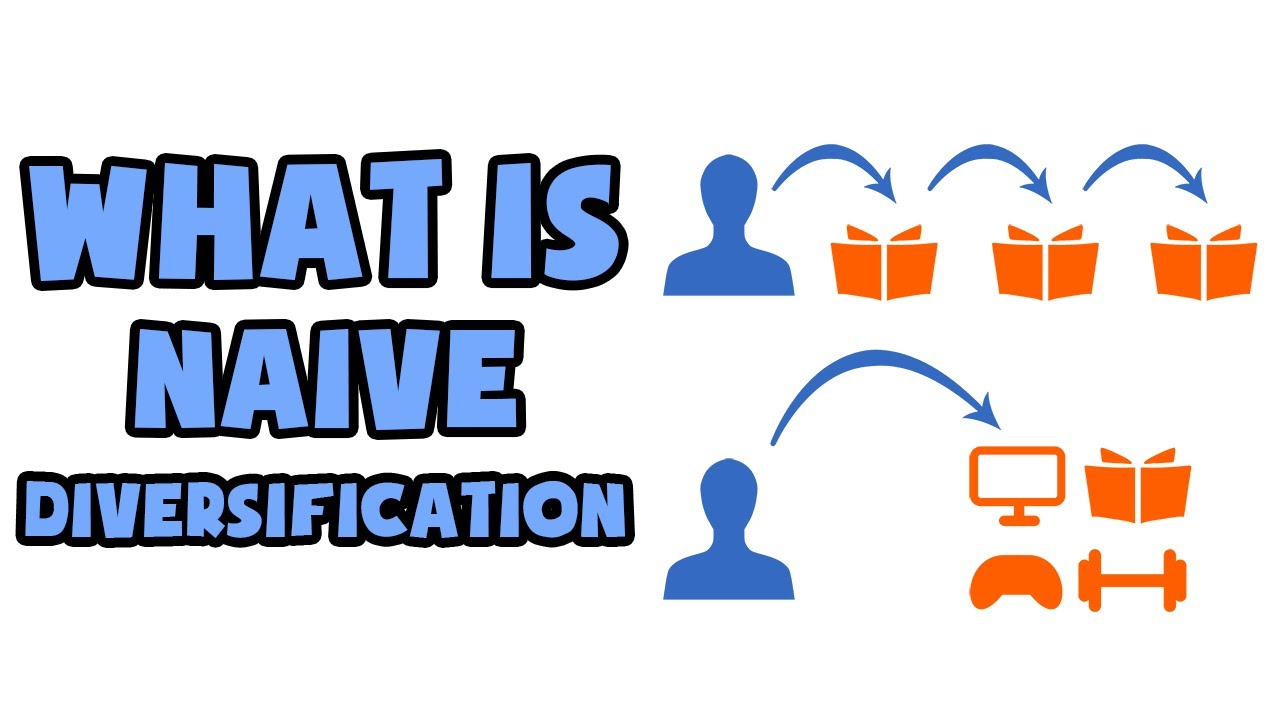
\includegraphics{figures/fig_0002.png}
\textgreater{} OCR cue: 5

\hypertarget{figure-3-slide-2}{%
\subsubsection{Figure 3 (Slide 2)}\label{figure-3-slide-2}}


\includegraphics{figures/fig_0003.jpg}

\hypertarget{figure-4-slide-16}{%
\subsubsection{Figure 4 (Slide 16)}\label{figure-4-slide-16}}

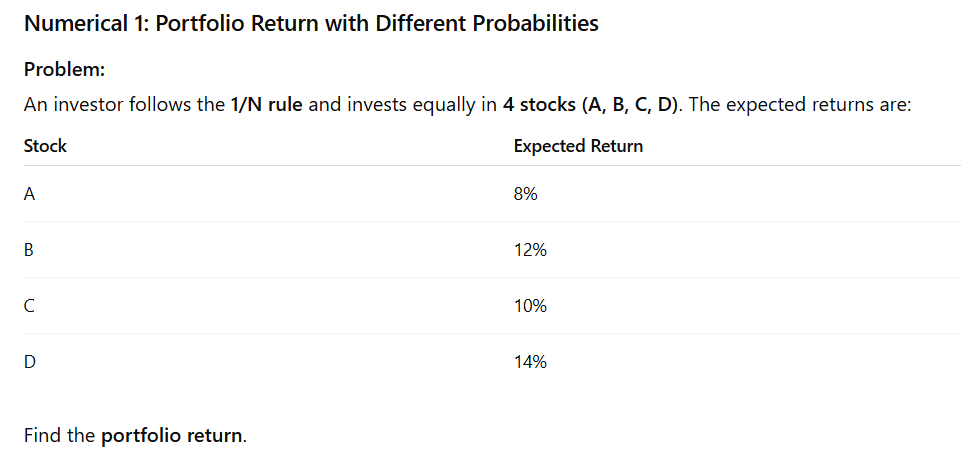
\includegraphics{figures/fig_0004.png}
\textgreater{} OCR cue: Numerical 1: Portfolio Return with Different
Probabilities Problem: An investor follows the 1/N rule and invests
equally in 4 stocks (A, B, C, D). The expected returns are: Stock A Find
the portfolio return. Expected Return 8\% 12\% 10\% 14\%

\hypertarget{figure-5-slide-17}{%
\subsubsection{Figure 5 (Slide 17)}\label{figure-5-slide-17}}

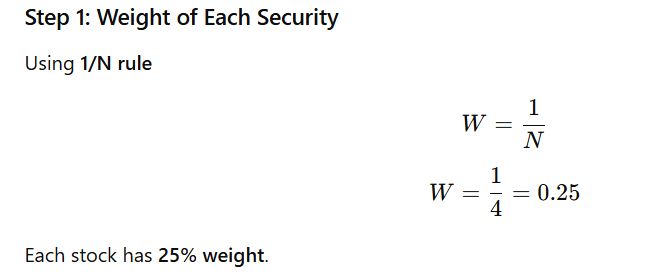
\includegraphics{figures/fig_0005.png}
\textgreater{} OCR cue: Step 1: Weight of Each Security Using 1/N rule
Each stock has 25\% weight.

\hypertarget{figure-6-slide-18}{%
\subsubsection{Figure 6 (Slide 18)}\label{figure-6-slide-18}}

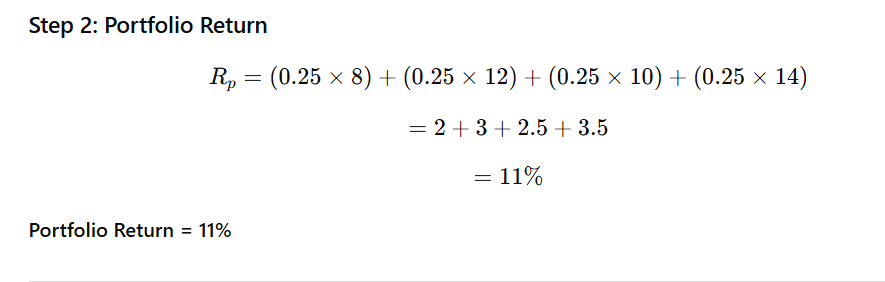
\includegraphics{figures/fig_0006.png}
\textgreater{} OCR cue: Step 2: Portfolio Return R, = (0.25 x 8) + (0.25
x 12) + (0.25 x 10) + (0.25 x 14) =24+34+2.543.5 = 11\% Portfolio Return
= 11\%

\hypertarget{figure-7-slide-19}{%
\subsubsection{Figure 7 (Slide 19)}\label{figure-7-slide-19}}

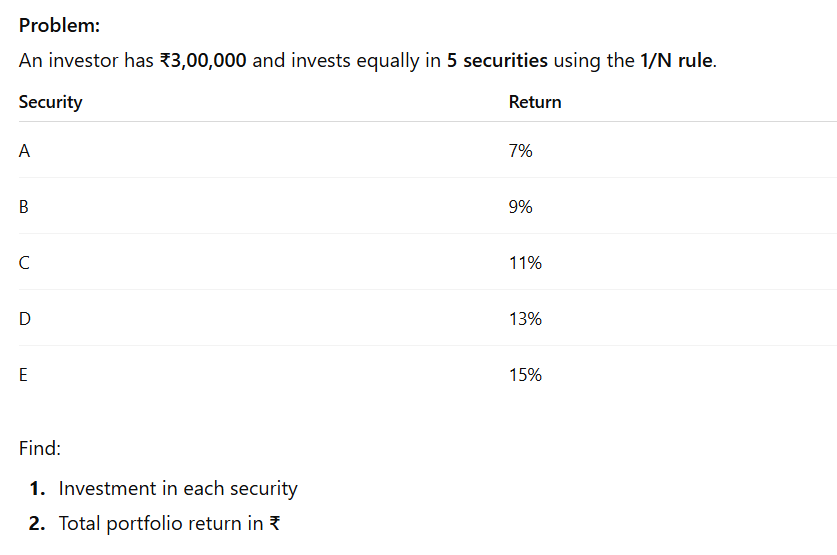
\includegraphics{figures/fig_0007.png}
\textgreater{} OCR cue: Problem: An investor has 3,00,000 and invests
equally in 5 securities using the 1/N rule. Security Return A 7\% B 9\%
Cc 11\% D 13\% E 15\% Find: 1. Investment in each security 2. Total
portfolio return in =

\hypertarget{figure-8-slide-20}{%
\subsubsection{Figure 8 (Slide 20)}\label{figure-8-slide-20}}

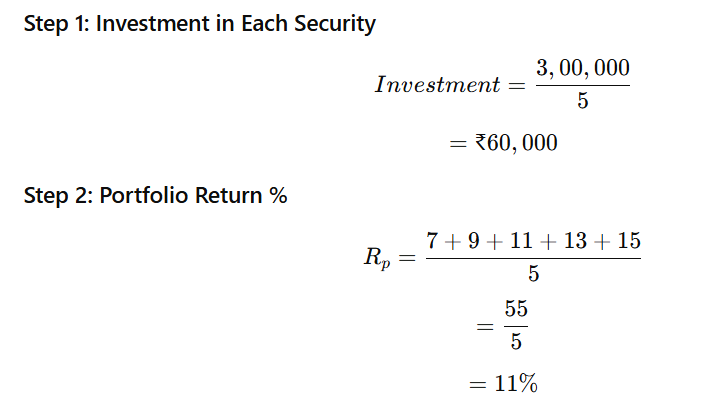
\includegraphics{figures/fig_0008.png}
\textgreater{} OCR cue: Step 1: Investment in Each Security Investment =
--- = \%60, 000 Step 2: Portfolio Return \% p= ee 13 +15 \_ 5 5 = 11\%

\hypertarget{figure-9-slide-21}{%
\subsubsection{Figure 9 (Slide 21)}\label{figure-9-slide-21}}

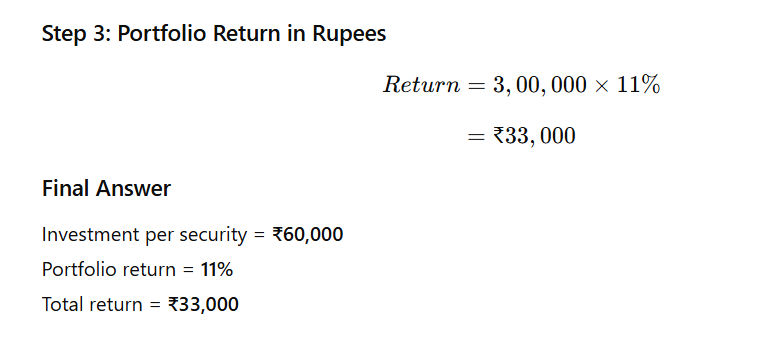
\includegraphics{figures/fig_0009.png}
\textgreater{} OCR cue: Step 3: Portfolio Return in Rupees Return =
3,00, 000 x 11\% = \%33, 000 Final Answer Investment per security =
60,000 Portfolio return = 11\% Total return = 33,000

\hypertarget{unit-410-rolling-covariance-windows.pptx}{%
\subsection{UNIT 4/10 Rolling Covariance
Windows.pptx}\label{unit-410-rolling-covariance-windows.pptx}}

\hypertarget{figure-1-slide-3}{%
\subsubsection{Figure 1 (Slide 3)}\label{figure-1-slide-3}}

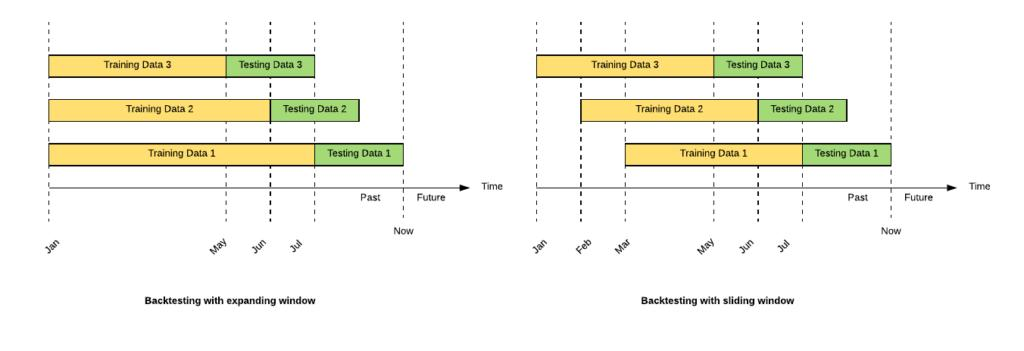
\includegraphics{figures/fig_0010.png}
\textgreater{} OCR cue: Past Backtosting with sliding window Backtesting
with expanding window

\hypertarget{figure-2-slide-12}{%
\subsubsection{Figure 2 (Slide 12)}\label{figure-2-slide-12}}

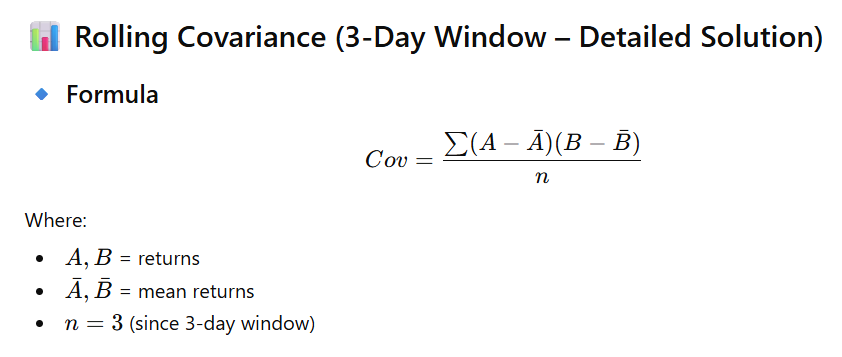
\includegraphics{figures/fig_0011.png}
\textgreater{} OCR cue: 'al Rolling Covariance (3-Day Window ---
Detailed Solution) ¢@ Formula \_ S(4\textasciitilde4)(B-B) Cov Where: e
A,B = returns . A, B = mean returns * n= 3 (since 3-day window)

\hypertarget{figure-3-slide-13}{%
\subsubsection{Figure 3 (Slide 13)}\label{figure-3-slide-13}}

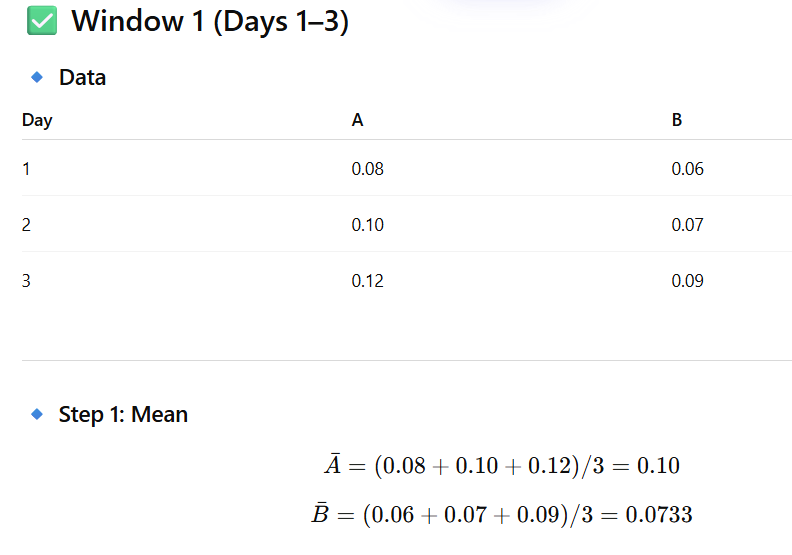
\includegraphics{figures/fig_0012.png}
\textgreater{} OCR cue: Window 1 (Days 1-3) ¢ Data Day 1 ¢ Step 1: Mean
0.08 0.10 0.12 0.06 0.07 0.09 A = (0.08 + 0.10 + 0.12)/3 = 0.10 B =
(0.06 + 0.07 + 0.09)/3 = 0.0733

\hypertarget{figure-4-slide-14}{%
\subsubsection{Figure 4 (Slide 14)}\label{figure-4-slide-14}}

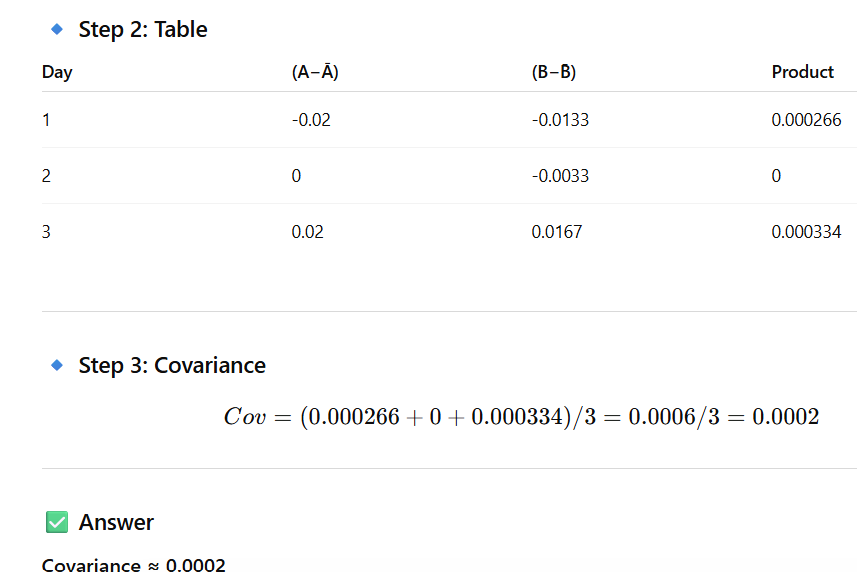
\includegraphics{figures/fig_0013.png}
\textgreater{} OCR cue: ¢ Step 2: Table Day (A-A) (B-B) 1 -0.02 -0.0133
2 0 -0.0033 3 0.02 0.0167 ¢@ Step 3: Covariance Product 0.000266
0.000334 Cov = (0.000266 + 0 + 0.000334)/3 = 0.0006/3 = 0.0002 Answer
Covariance = 0.0002

\hypertarget{figure-5-slide-15}{%
\subsubsection{Figure 5 (Slide 15)}\label{figure-5-slide-15}}

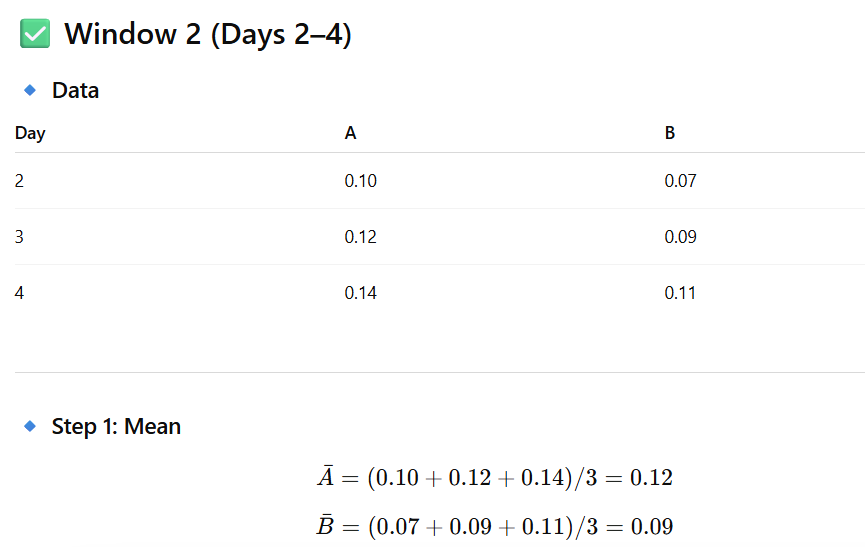
\includegraphics{figures/fig_0014.png}
\textgreater{} OCR cue: Window 2 (Days 2-4) ¢ Data Day 2 3 4 ¢ Step 1:
Mean 0.10 0.12 0.14 0.07 0.09 0.11 A= (0.10 + 0.12 + 0.14)/3 = 0.12 B =
(0.07 + 0.09 + 0.11)/3 = 0.09

\hypertarget{figure-6-slide-16}{%
\subsubsection{Figure 6 (Slide 16)}\label{figure-6-slide-16}}

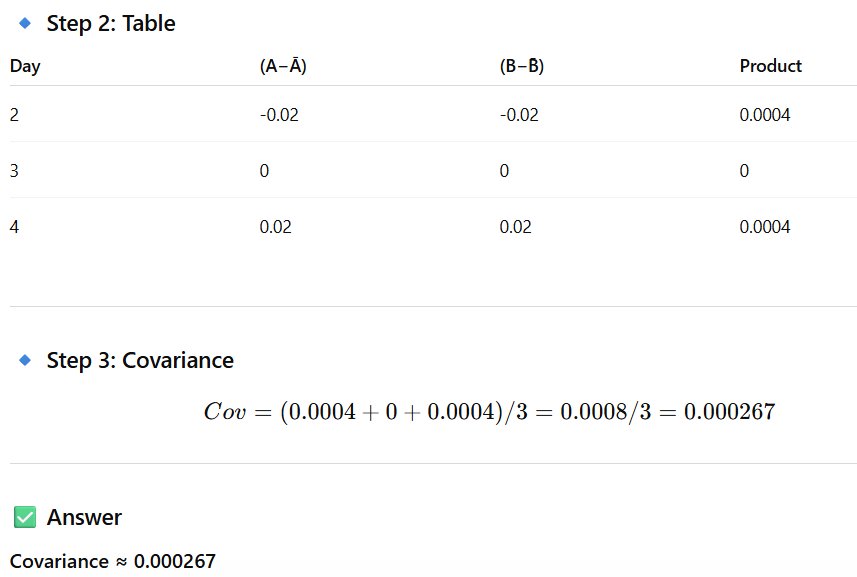
\includegraphics{figures/fig_0015.png}
\textgreater{} OCR cue: ¢ Step 2: Table Day (a-A) (6-8) 2 -0.02 -0.02 3
0 0 4 0.02 0.02 ¢@ Step 3: Covariance Product 0.0004 0.0004 Cov =
(0.0004 + 0 + 0.0004) /3 = 0.0008/3 = 0.000267 Answer Covariance =
0.000267

\hypertarget{figure-7-slide-17}{%
\subsubsection{Figure 7 (Slide 17)}\label{figure-7-slide-17}}

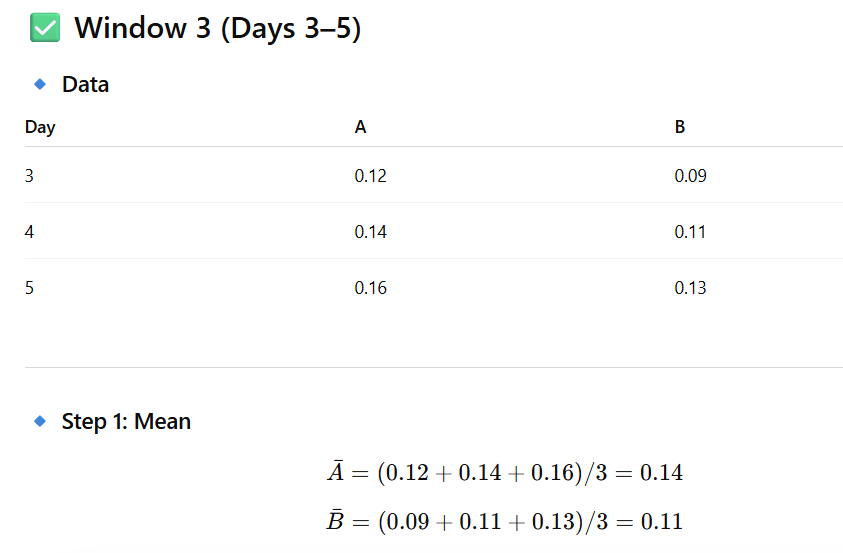
\includegraphics{figures/fig_0016.png}
\textgreater{} OCR cue: Window 3 (Days 3-5) ¢ Data Day 3 ¢ Step 1: Mean
0.12 0.14 0.16 0.09 0.11 0.13 A= (0.12 + 0.14 + 0.16)/3 = 0.14 B = (0.09
+ 0.11 + 0.13)/3 = 0.11

\hypertarget{figure-8-slide-18}{%
\subsubsection{Figure 8 (Slide 18)}\label{figure-8-slide-18}}

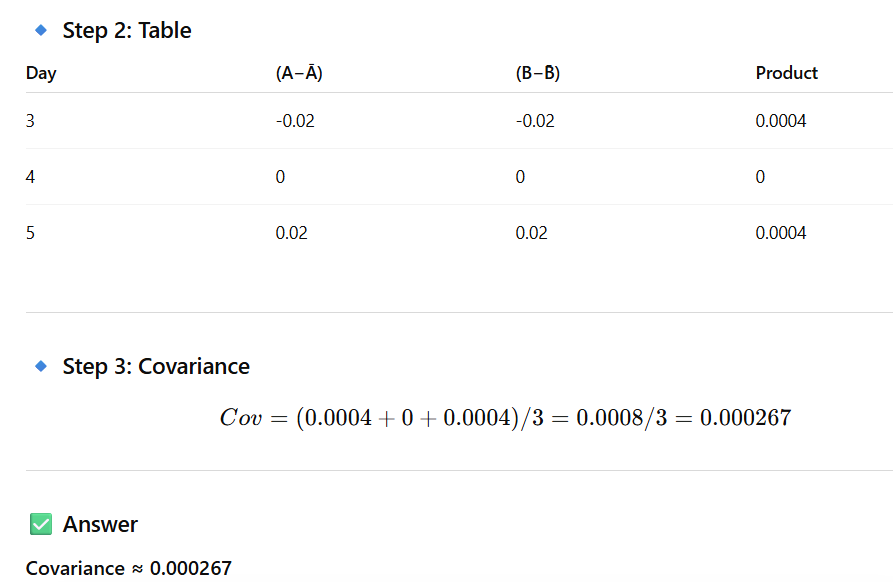
\includegraphics{figures/fig_0017.png}
\textgreater{} OCR cue: ¢ Step 2: Table Day 3 ¢@ Step 3: Covariance
(A-A) -0.02 0.02 (B-B) -0.02 0.02 Product 0.0004 0.0004 Cov = (0.0004 +
0 + 0.0004) /3 = 0.0008/3 = 0.000267 Answer Covariance * 0.000267

\hypertarget{figure-9-slide-19}{%
\subsubsection{Figure 9 (Slide 19)}\label{figure-9-slide-19}}

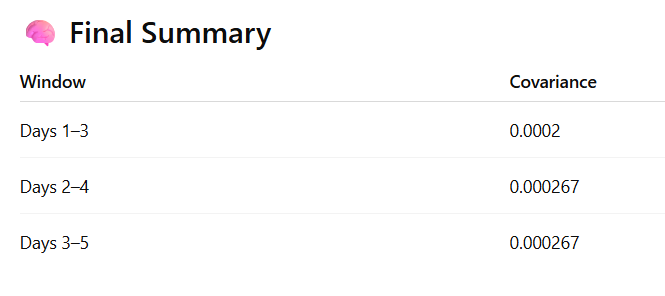
\includegraphics{figures/fig_0018.png}
\textgreater{} OCR cue: © Final Summary Window Days 1-3 Days 2-4 Days
3-5 Covariance 0.0002 0.000267 0.000267

\hypertarget{figure-10-slide-22}{%
\subsubsection{Figure 10 (Slide 22)}\label{figure-10-slide-22}}

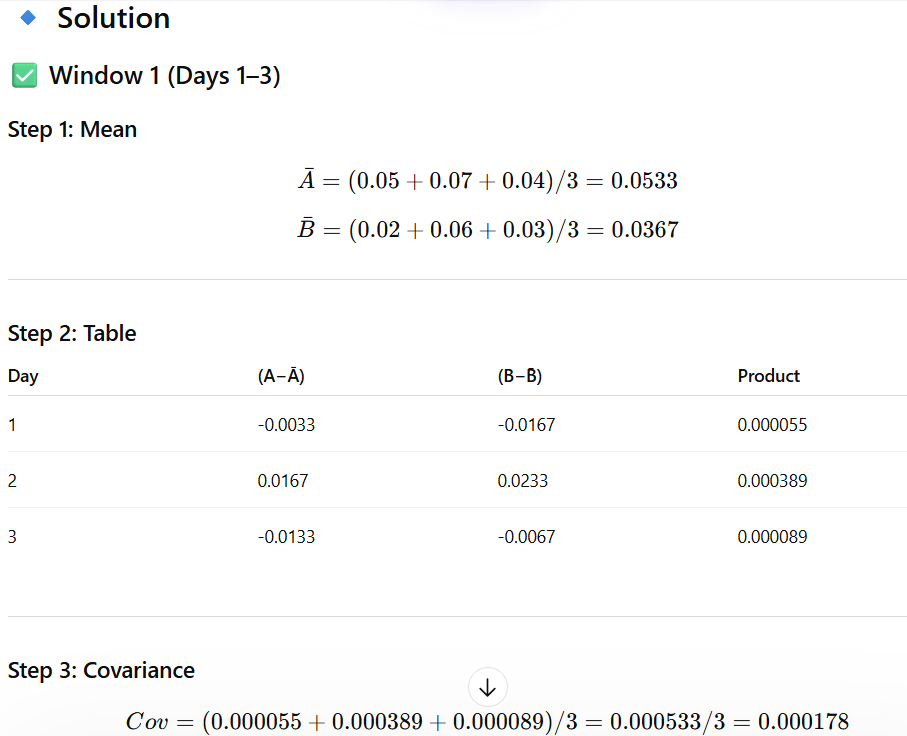
\includegraphics{figures/fig_0019.png}
\textgreater{} OCR cue: ¢@ Solution Window 1 (Days 1-3) Step 1: Mean A =
(0.05 + 0.07 + 0.04)/3 = 0.0533 B = (0.02 + 0.06 + 0.03)/3 = 0.0367 Step
2: Table Day (A-A) (B-B) Product 1 -0.0033 -0.0167 0.000055 2 0.0167
0.0233 0.000389 3 -0.0133 -0.0067 0.000089 Step 3: Covariance Vv Cov =
(0.000055 + 0.000389 + 0.000089) /3 = 0.000533/3 = 0.000178

\hypertarget{figure-11-slide-23}{%
\subsubsection{Figure 11 (Slide 23)}\label{figure-11-slide-23}}

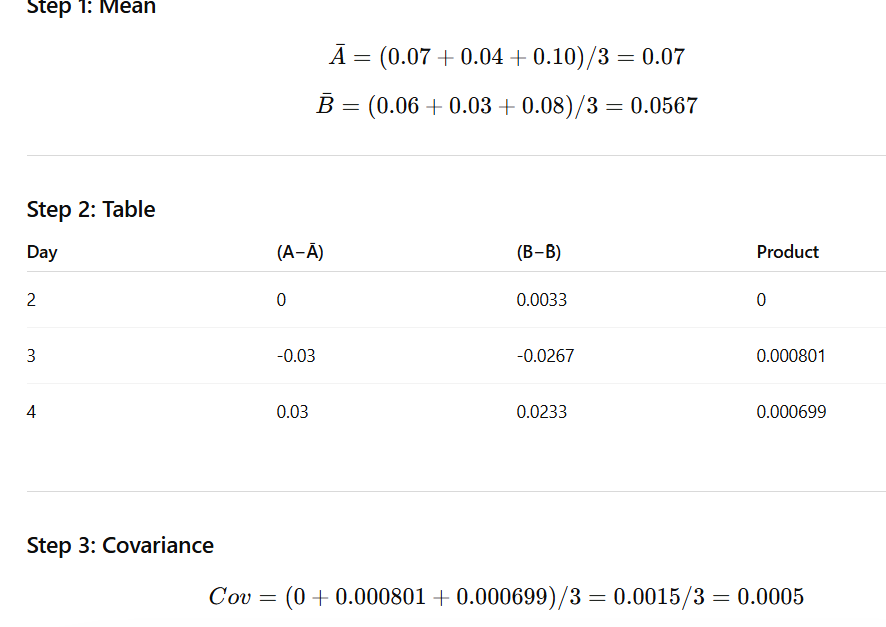
\includegraphics{figures/fig_0020.png}
\textgreater{} OCR cue: step I. viean A = (0.07 + 0.04 + 0.10)/3 = 0.07
B = (0.06 + 0.03 + 0.08)/3 = 0.0567 Step 2: Table Day (a-A) (B-B)
Product 2 0 0.0033 0 3 -0.03 -0.0267 0.000801 4 0.03 0.0233 0.000699
Step 3: Covariance Cov = (0 + 0.000801 + 0.000699) /3 = 0.0015/3 =
0.0005

\hypertarget{figure-12-slide-24}{%
\subsubsection{Figure 12 (Slide 24)}\label{figure-12-slide-24}}

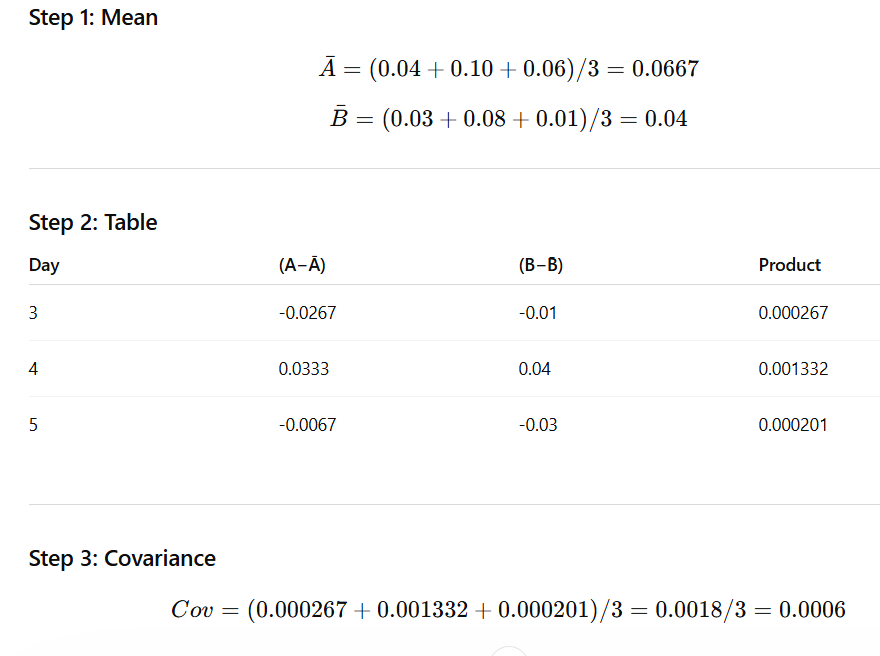
\includegraphics{figures/fig_0021.png}
\textgreater{} OCR cue: Step 1: Mean A= (0.04 + 0.10 + 0.06)/3 = 0.0667
B = (0.03 + 0.08 + 0.01)/3 = 0.04 Step 2: Table Day (A-A) (B-B) Product
3 -0.0267 -0.01 0.000267 4 0.0333 0.04 0.001332 5 -0.0067 -0.03 0.000201
Step 3: Covariance Cov = (0.000267 + 0.001332 + 0.000201) /3 = 0.0018/3
= 0.0006

\hypertarget{figure-13-slide-25}{%
\subsubsection{Figure 13 (Slide 25)}\label{figure-13-slide-25}}

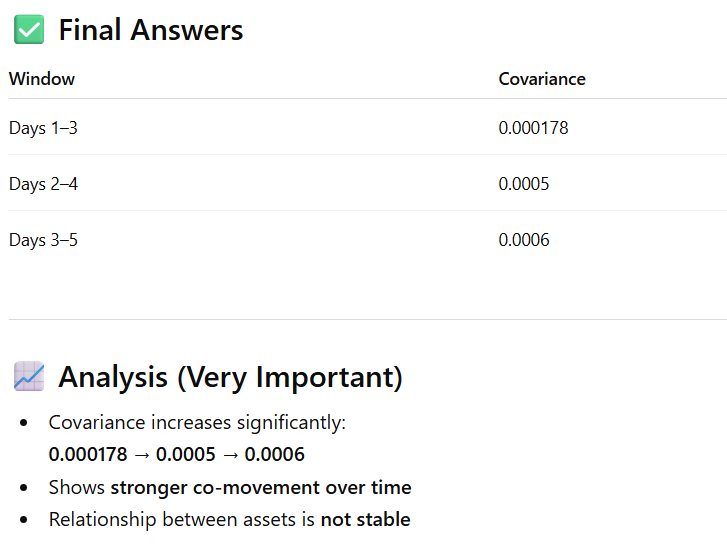
\includegraphics{figures/fig_0022.png}
\textgreater{} OCR cue: Final Answers Window Covariance Days 1-3
0.000178 Days 2-4 0.0005 Days 3-5 0.0006 -\textasciitilde{} Analysis
(Very Important) © Covariance increases significantly: 0.000178 ---
0.0005 --- 0.0006 * Shows stronger co-movement over time * Relationship
between assets is not stable

\hypertarget{figure-14-slide-26}{%
\subsubsection{Figure 14 (Slide 26)}\label{figure-14-slide-26}}

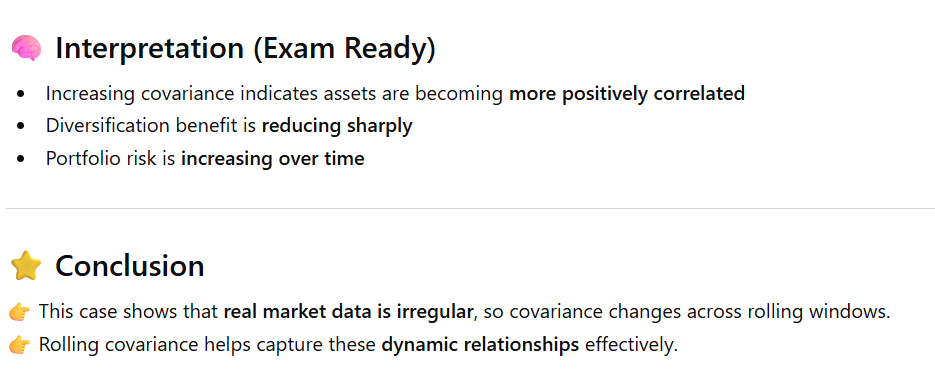
\includegraphics{figures/fig_0023.png}
\textgreater{} OCR cue: © Interpretation (Exam Ready) ¢ Increasing
covariance indicates assets are becoming more positively correlated ©
Diversification benefit is reducing sharply © Portfolio risk is
increasing over time wW Conclusion © This case shows that real market
data is irregular, so covariance changes across rolling windows. ©
Rolling covariance helps capture these dynamic relationships
effectively.

\hypertarget{unit-411-comparing-optimization-diversification-approaches_-empirical-comparison.pptx}{%
\subsection{UNIT 4/11 Comparing optimization \& diversification
approaches\_ Empirical
comparison.pptx}\label{unit-411-comparing-optimization-diversification-approaches_-empirical-comparison.pptx}}

\hypertarget{figure-1-slide-7}{%
\subsubsection{Figure 1 (Slide 7)}\label{figure-1-slide-7}}

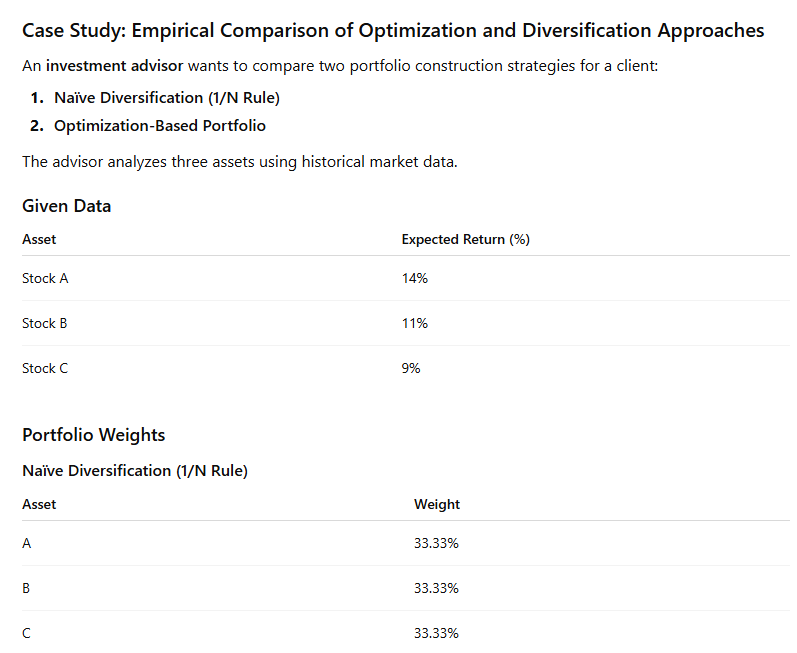
\includegraphics{figures/fig_0123.png}
\textgreater{} OCR cue: Case Study: Empirical Comparison of Optimization
and Diversification Approaches An investment advisor wants to compare
two portfolio construction strategies for a client: 1. Naive
Diversification (1/N Rule) 2. Optimization-Based Portfolio The advisor
analyzes three assets using historical market data. Given Data Asset
Expected Return (\%) Stock A 14\% Stock B 11\% Stock C 9\% Portfolio
Weights Naive D

\hypertarget{figure-2-slide-8}{%
\subsubsection{Figure 2 (Slide 8)}\label{figure-2-slide-8}}

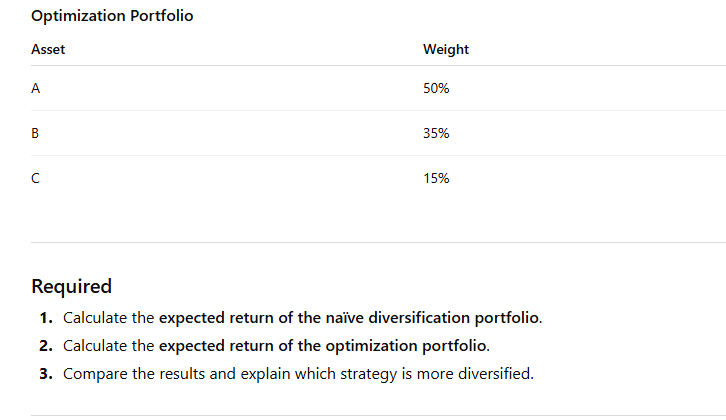
\includegraphics{figures/fig_0124.png}
\textgreater{} OCR cue: Optimization Portfolio Asset Weight A 50\% B
35\% c 15\% Required 1. Calculate the expected return of the naive
diversification portfolio. 2. Calculate the expected return of the
optimization portf 3. Compare the results and explain which strategy is
more diversified.

\hypertarget{figure-3-slide-9}{%
\subsubsection{Figure 3 (Slide 9)}\label{figure-3-slide-9}}

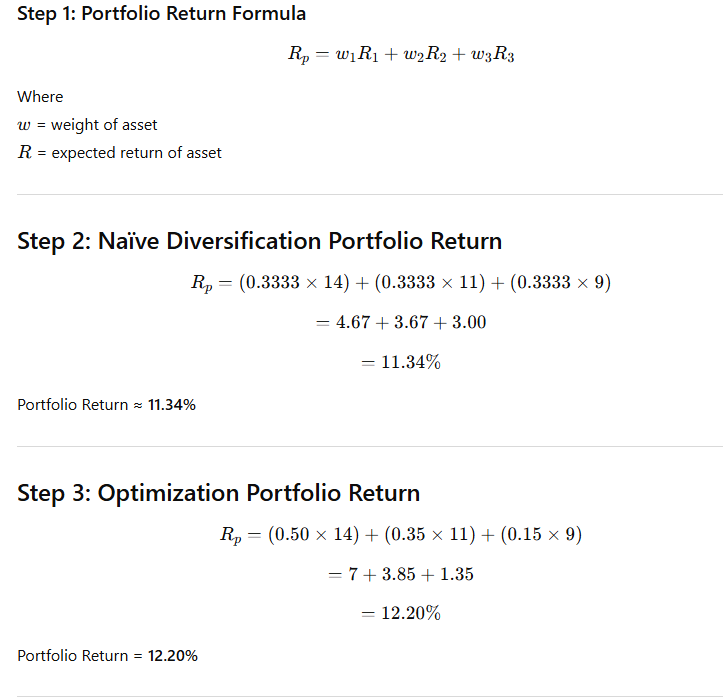
\includegraphics{figures/fig_0125.png}
\textgreater{} OCR cue: Step 1: Portfolio Return Formula Ry = wR, + weRe
+ w3Ry Where w = weight of asset R = expected return of asset Step 2:
Naive Diversification Portfolio Return R, = (0.3333 x 14) + (0.3333 x
11) + (0.3333 x 9) = 4.67 + 3.67 + 3.00 = 11.34\% Portfolio Return =
11.34\% Step 3: Optimization Portfolio Return Ry, = (0.50 x 14) + (0.35
x 11) + (0.15 x 9) = 743.85 +135 = 12.20\% Portfolio Return = 12.20\%

\hypertarget{figure-4-slide-10}{%
\subsubsection{Figure 4 (Slide 10)}\label{figure-4-slide-10}}

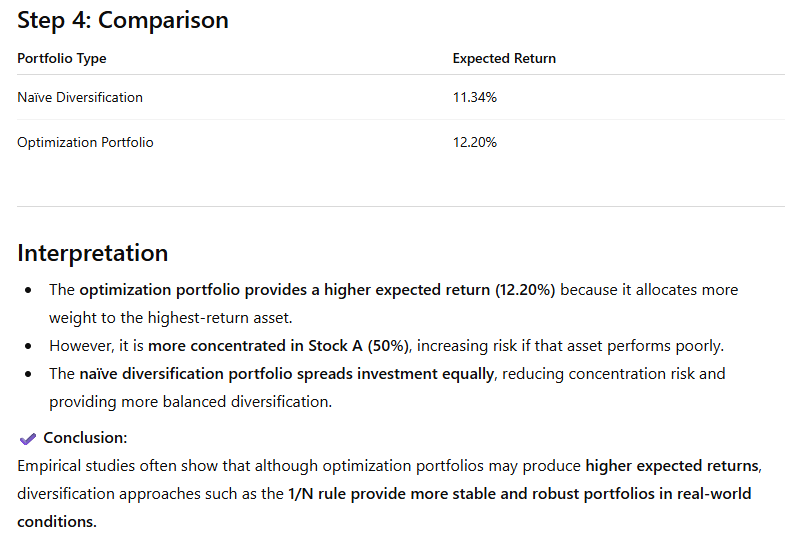
\includegraphics{figures/fig_0126.png}
\textgreater{} OCR cue: Step 4: Comparison Portfolio Type Expected
Return Naive Diversification 11.34\% Optimization Portfolio 12.20\%
Interpretation * The optimization portfolio provides a higher expected
return (12.20\%) because it allocates more weight to the highest-return
asset. * However, it is more concentrated in Stock A (50\%), increasing
risk if that asset performs poorly. * The naive diversification
portfolio spre

\hypertarget{unit-44-what-is-a-risk-budget.docx}{%
\subsection{UNIT 4/4 What is a Risk
Budget.docx}\label{unit-44-what-is-a-risk-budget.docx}}

\hypertarget{figure-1-image}{%
\subsubsection{Figure 1 (Image)}\label{figure-1-image}}

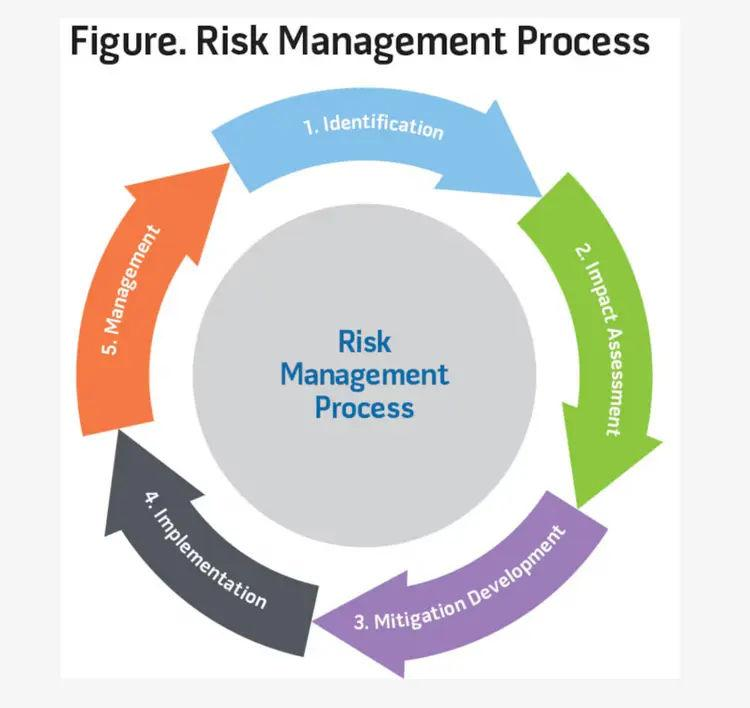
\includegraphics{figures/fig_0024.jpeg}
\textgreater{} OCR cue: Figure. Risk Management Process st
identificatio, 2 wr quaussassv ped

\hypertarget{unit-45-risk-budgeting-numericals.pptx}{%
\subsection{UNIT 4/5 Risk Budgeting
Numericals.pptx}\label{unit-45-risk-budgeting-numericals.pptx}}

\hypertarget{figure-1-slide-2}{%
\subsubsection{Figure 1 (Slide 2)}\label{figure-1-slide-2}}

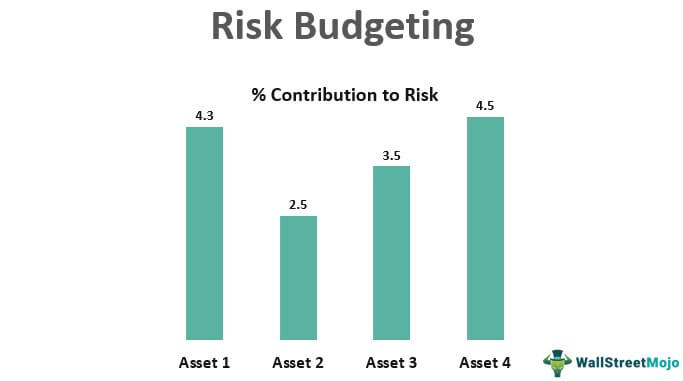
\includegraphics{figures/fig_0025.png}
\textgreater{} OCR cue: Risk Budgeting \% Contribution to Risk =, 43 35
\textbar{} Asset1 --- Asset2-«Asset3. «Asset 4 ``E\textgreater{}
WallstreetMojo

\hypertarget{unit-46-simplified-risk-parity-portfolios.pptx}{%
\subsection{UNIT 4/6 Simplified Risk Parity
Portfolios.pptx}\label{unit-46-simplified-risk-parity-portfolios.pptx}}

\hypertarget{figure-1-slide-7-1}{%
\subsubsection{Figure 1 (Slide 7)}\label{figure-1-slide-7-1}}

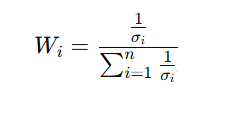
\includegraphics{figures/fig_0026.png}

\hypertarget{figure-2-slide-11}{%
\subsubsection{Figure 2 (Slide 11)}\label{figure-2-slide-11}}

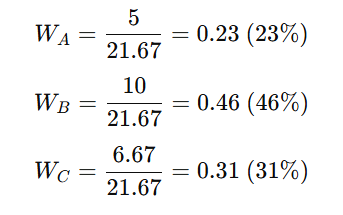
\includegraphics{figures/fig_0027.png}
\textgreater{} OCR cue: Wa 5 = ---``--- = 0.23 (23\% Wa ser (23\%) 10 =
= 0.46 (46\% a67 9 (46\%) 6.67 = ------* =0.31 (31\% ©\textasciitilde{}
31.67 (31\%)

\hypertarget{figure-3-slide-13-1}{%
\subsubsection{Figure 3 (Slide 13)}\label{figure-3-slide-13-1}}

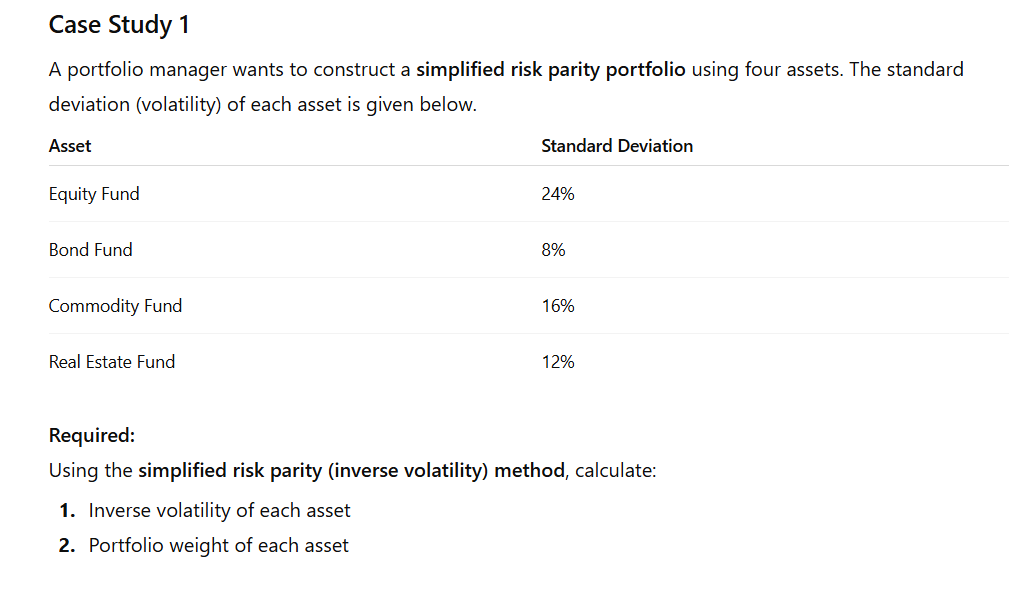
\includegraphics{figures/fig_0028.png}
\textgreater{} OCR cue: Case Study 1 A portfolio manager wants to
construct a simplified risk parity portfolio using four assets. The
standard deviation (volatility) of each asset is given below. Asset
Standard Deviation Equity Fund 24\% Bond Fund 8\% Commodity Fund 16\%
Real Estate Fund 12\% Required: Using the simplified risk parity
(inverse volatility) method, calculate: 1. Inverse volatility of each
asset 2. Portfolio we

\hypertarget{figure-4-slide-14-1}{%
\subsubsection{Figure 4 (Slide 14)}\label{figure-4-slide-14-1}}

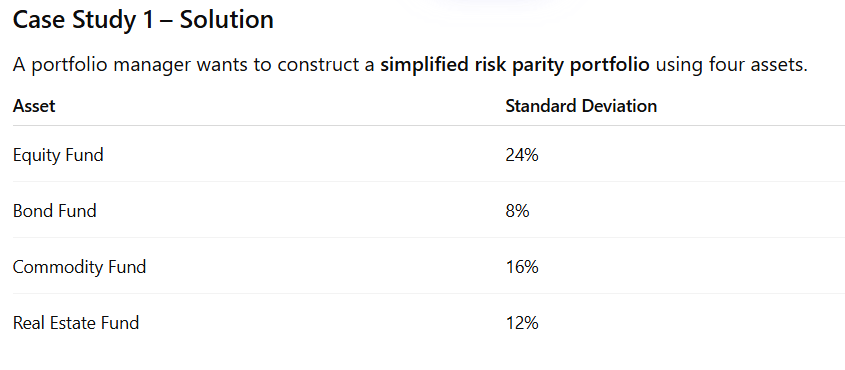
\includegraphics{figures/fig_0029.png}
\textgreater{} OCR cue: Case Study 1 - Solution A portfolio manager
wants to construct a simplified risk parity portfolio using four assets.
Asset Standard Deviation Equity Fund 24\% Bond Fund 8\% Commodity Fund
16\% Real Estate Fund 12\%

\hypertarget{figure-5-slide-15-1}{%
\subsubsection{Figure 5 (Slide 15)}\label{figure-5-slide-15-1}}

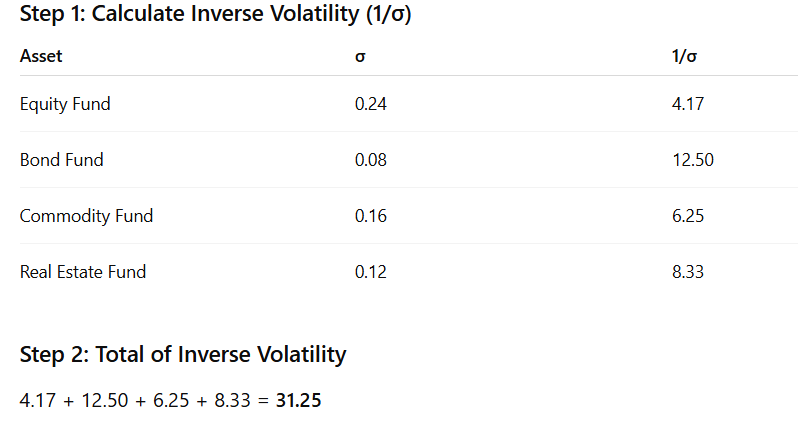
\includegraphics{figures/fig_0030.png}
\textgreater{} OCR cue: Step 1: Calculate Inverse Volatility (1/0) Asset
° Vo Equity Fund 0.24 4q7 Bond Fund 0.08 12.50 Commodity Fund 0.16 6.25
Real Estate Fund 0.12 833 Step 2: Total of Inverse Volatility 4.17 +
12.50 + 6.25 + 8.33 = 31.25

\hypertarget{figure-6-slide-16-1}{%
\subsubsection{Figure 6 (Slide 16)}\label{figure-6-slide-16-1}}

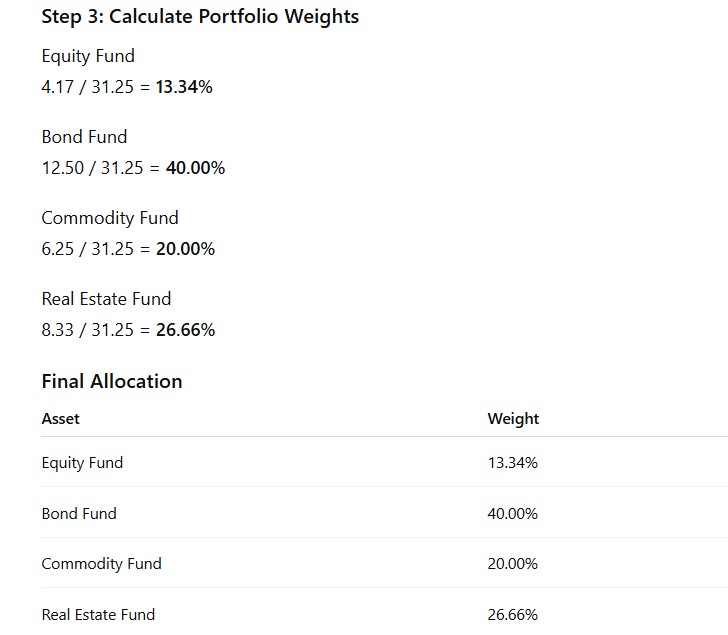
\includegraphics{figures/fig_0031.png}
\textgreater{} OCR cue: Step 3: Calculate Portfolio Weights Equity Fund
4.7 / 31.25 = 13.34\% Bond Fund 12.50 / 31.25 = 40.00\% Commodity Fund
6.25 / 31.25 = 20.00\% Real Estate Fund 8.33 / 31.25 = 26.66\% Final
Allocation Asset Equity Fund Bond Fund Commodity Fund Real Estate Fund
Weight 13.34\% 20.00\% 26.66\%

\hypertarget{figure-7-slide-17-1}{%
\subsubsection{Figure 7 (Slide 17)}\label{figure-7-slide-17-1}}

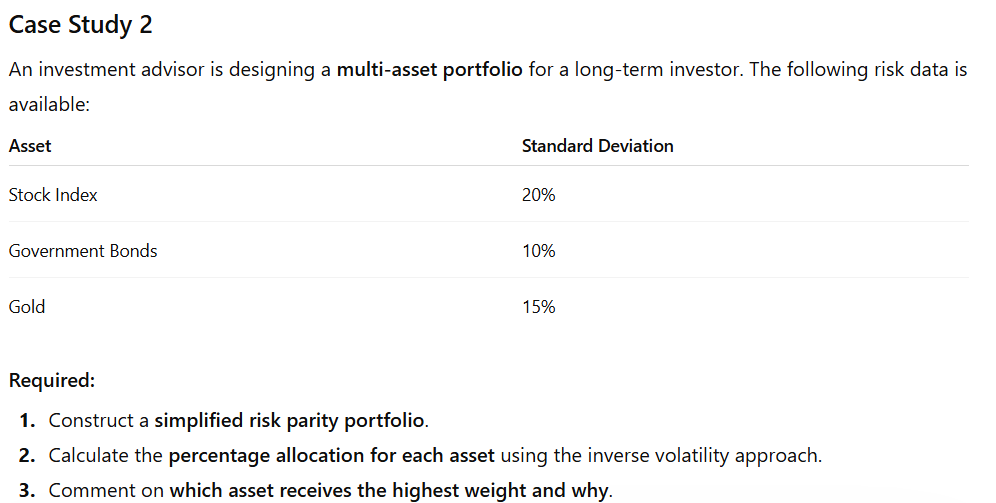
\includegraphics{figures/fig_0032.png}
\textgreater{} OCR cue: Case Study 2 An investment advisor is designing
a multi-asset portfolio for a long-term investor. The following risk
data is available: Asset Standard Deviation Stock Index 20\% Government
Bonds 10\% Gold 15\% Required: 1. Construct a simplified risk parity
portfolio. 2. Calculate the percentage allocation for each asset using
the inverse volatility approach. 3. Comment on which asset receives the
hi

\hypertarget{figure-8-slide-18-1}{%
\subsubsection{Figure 8 (Slide 18)}\label{figure-8-slide-18-1}}

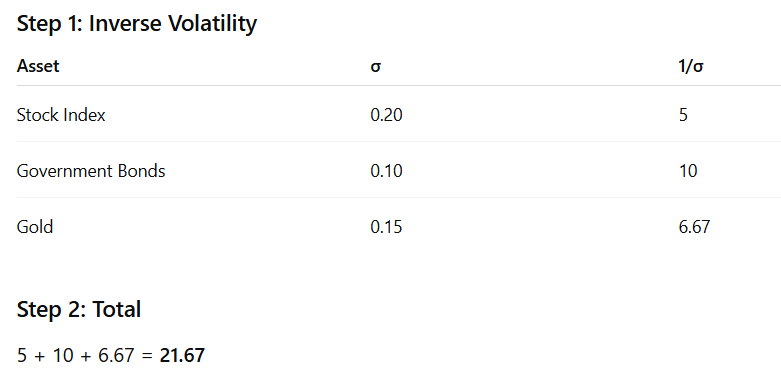
\includegraphics{figures/fig_0033.png}
\textgreater{} OCR cue: Step 1: Inverse Volatility Asset Stock Index
Government Bonds Gold Step 2: Total 5 + 10 + 6.67 = 21.67 0.20 0.10 0.15
Vo 6.67

\hypertarget{figure-9-slide-19-1}{%
\subsubsection{Figure 9 (Slide 19)}\label{figure-9-slide-19-1}}

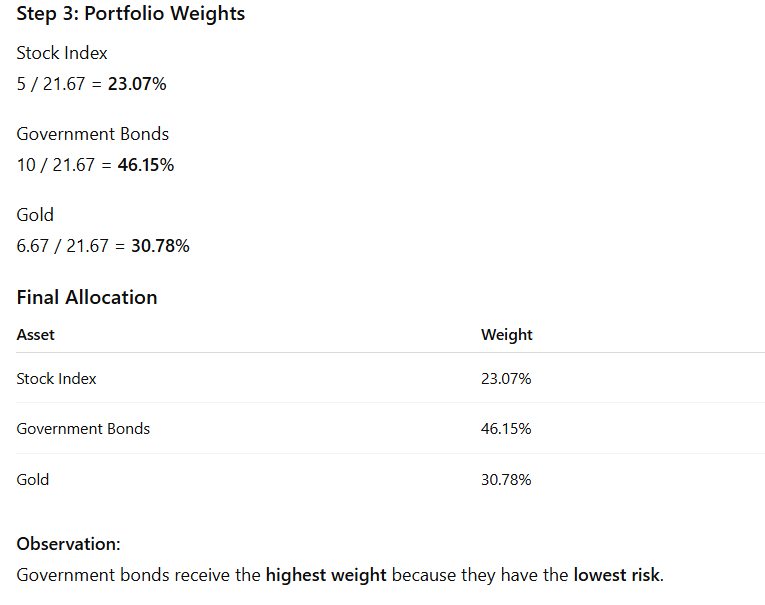
\includegraphics{figures/fig_0034.png}
\textgreater{} OCR cue: Step 3: Portfolio Weights Stock Index 5 / 21.67
= 23.07\% Government Bonds 10 / 21.67 = 46.15\% Gold 6.67 / 21.67 =
30.78\% Final Allocation Asset Weight Stock Index 23.07\% Government
Bonds 46.15\% Gold 30.78\% Observation: Government bonds receive the
highest weight because they have the lowest risk.

\hypertarget{figure-10-slide-20}{%
\subsubsection{Figure 10 (Slide 20)}\label{figure-10-slide-20}}

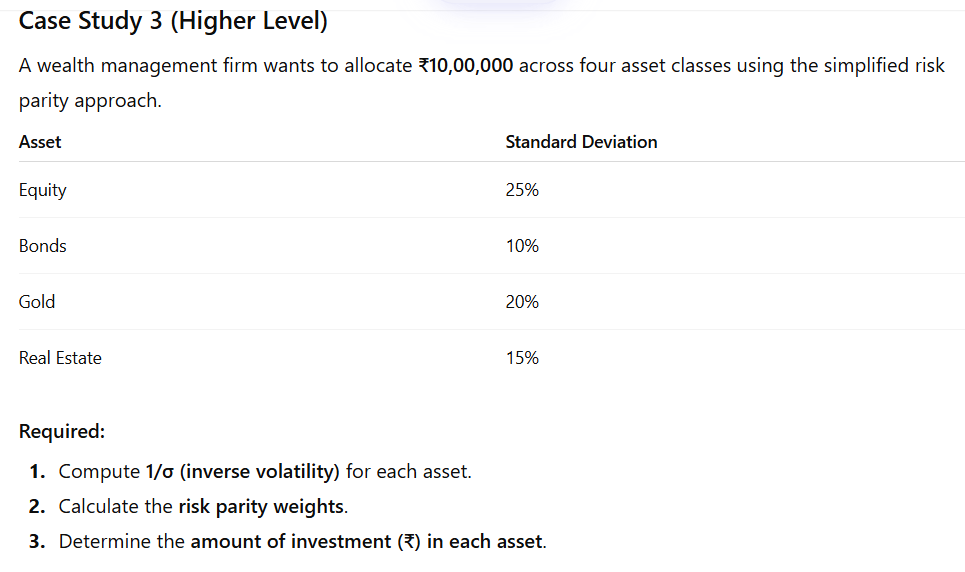
\includegraphics{figures/fig_0035.png}
\textgreater{} OCR cue: Case Study 3 (Higher Level) A wealth management
firm wants to allocate \%10,00,000 across four asset classes using the
simplified risk parity approach. Asset Standard Deviation Equity 25\%
Bonds 10\% Gold 20\% Real Estate 15\% Required: 1. Compute 1/c (inverse
volatility) for each asset. 2. Calculate the risk parity weights. 3.
Determine the amount of investment (\%) in each asset.

\hypertarget{figure-11-slide-21}{%
\subsubsection{Figure 11 (Slide 21)}\label{figure-11-slide-21}}

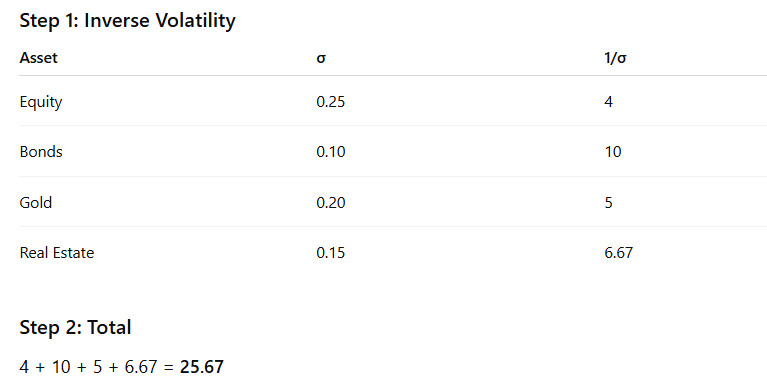
\includegraphics{figures/fig_0036.png}
\textgreater{} OCR cue: Step 1: Inverse Volatility Asset Equity Bonds
Gold Real Estate Step 2: Total 4+10+5 + 6.67 = 25.67 0.25 0.10 0.20 0.15
6.67

\hypertarget{figure-12-slide-22}{%
\subsubsection{Figure 12 (Slide 22)}\label{figure-12-slide-22}}

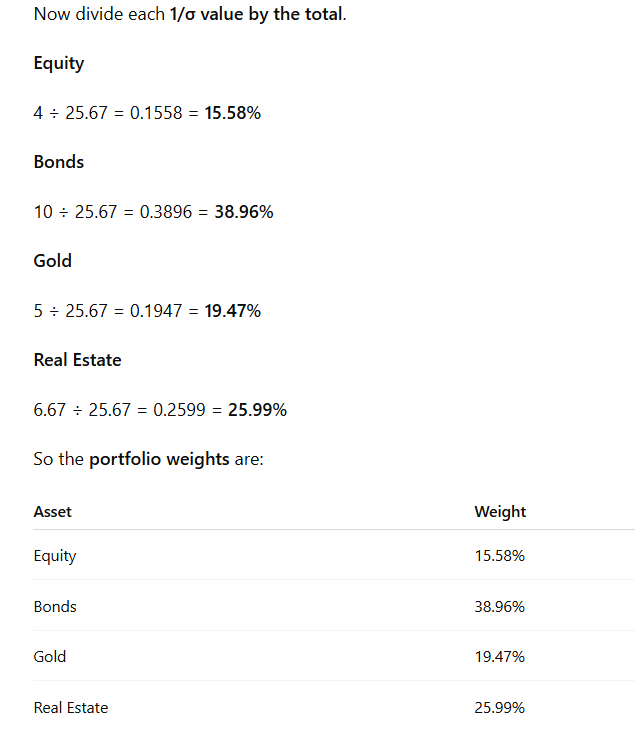
\includegraphics{figures/fig_0037.png}
\textgreater{} OCR cue: Now divide each 1/o value by the total. Equity 4
= 25.67 = 0.1558 = 15.58\% Bonds 10 + 25.67 = 0.3896 = 38.96\% Gold 5 +
25.67 = 0.1947 = 19.47\% Real Estate 6.67 = 25.67 = 0.2599 = 25.99\% So
the portfolio weights are: Asset Equity Bonds Gold Real Estate Weight
15.58\% 38.96\% 19.47\% 25.99\%

\hypertarget{figure-13-slide-23}{%
\subsubsection{Figure 13 (Slide 23)}\label{figure-13-slide-23}}

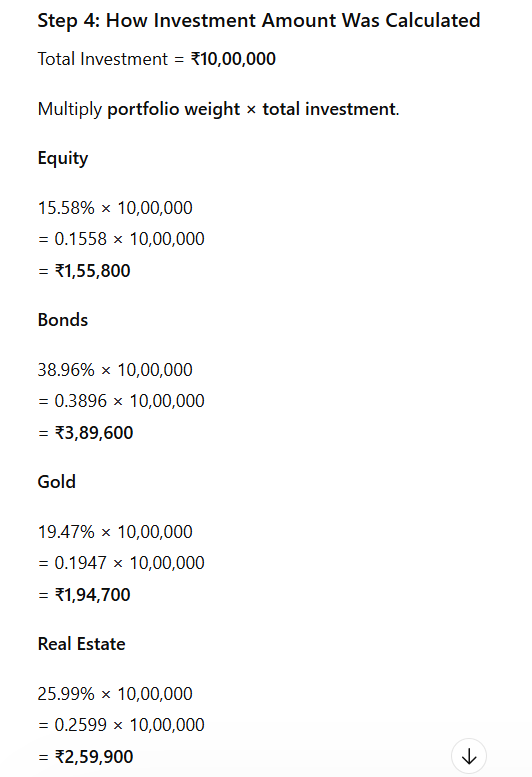
\includegraphics{figures/fig_0038.png}
\textgreater{} OCR cue: Step 4: How Investment Amount Was Calculated
Total Investment = 210,00,000 Multiply portfolio weight x total
investment. Equity 15.58\% x 10,00,000 = 0.1558 x 10,00,000 = \%1,55,800
Bonds 38.96\% x 10,00,000 = 0.3896 x 10,00,000 = \%3,89,600 Gold 19.47\%
x 10,00,000 = 0.1947 x 10,00,000 = \%1,94,700 Real Estate 25.99\% x
10,00,000 = 0.2599 x 10,00,000 = \%2,59,900 Vv

\hypertarget{figure-14-slide-24}{%
\subsubsection{Figure 14 (Slide 24)}\label{figure-14-slide-24}}

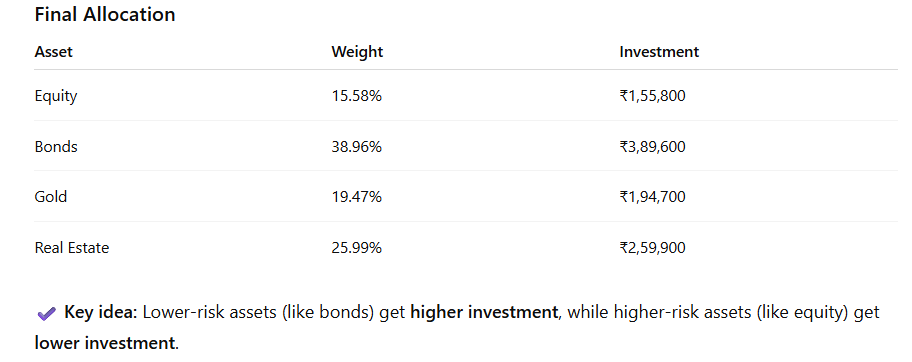
\includegraphics{figures/fig_0039.png}
\textgreater{} OCR cue: Final Allocation Asset Weight Investment Equity
15.58\% 31,55,800 Bonds 38.96\% 3,89,600 Gold 19.47\% 31,94,700 Real
Estate 25.99\% \%2,59,900 Vv Key idea: Lower-risk assets (like bonds)
get higher investment, while higher-risk assets (like equity) get lower
investment.

\hypertarget{figure-15-slide-25}{%
\subsubsection{Figure 15 (Slide 25)}\label{figure-15-slide-25}}

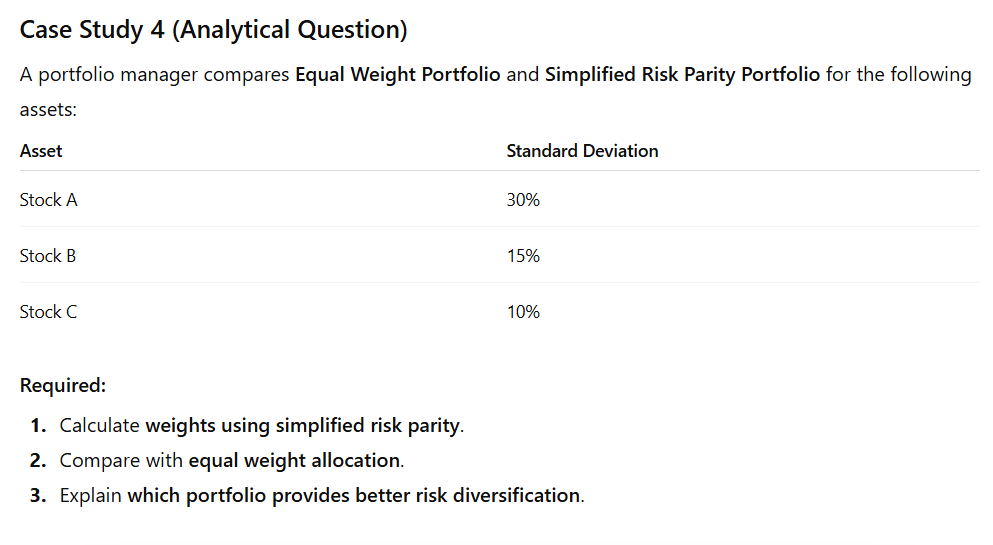
\includegraphics{figures/fig_0040.png}
\textgreater{} OCR cue: Case Study 4 (Analytical Question) A portfolio
manager compares Equal Weight Portfolio and Simplified Risk Parity
Portfolio for the following assets: Asset Standard Deviation Stock A
30\% Stock B 15\% Stock C 10\% Required: 1. Calculate weights using
simplified risk parity. 2. Compare with equal weight allocation. 3.
Explain which portfolio provides better risk diversification.

\hypertarget{figure-16-slide-26}{%
\subsubsection{Figure 16 (Slide 26)}\label{figure-16-slide-26}}

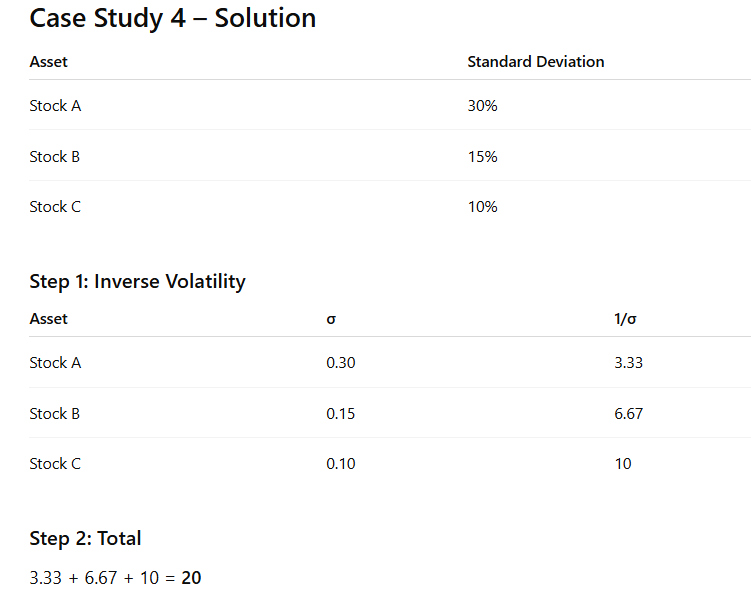
\includegraphics{figures/fig_0041.png}
\textgreater{} OCR cue: Case Study 4 --- Solution Asset Stock A Stock B
Stock C Step 1: Inverse Volatility Asset ° Stock A 0.30 Stock B 0.15
Stock C 0.10 Step 2: Total 3.33 + 6.67 + 10 = 20 Standard Deviation 30\%
15\% 10\% 3.33 6.67

\hypertarget{figure-17-slide-27}{%
\subsubsection{Figure 17 (Slide 27)}\label{figure-17-slide-27}}

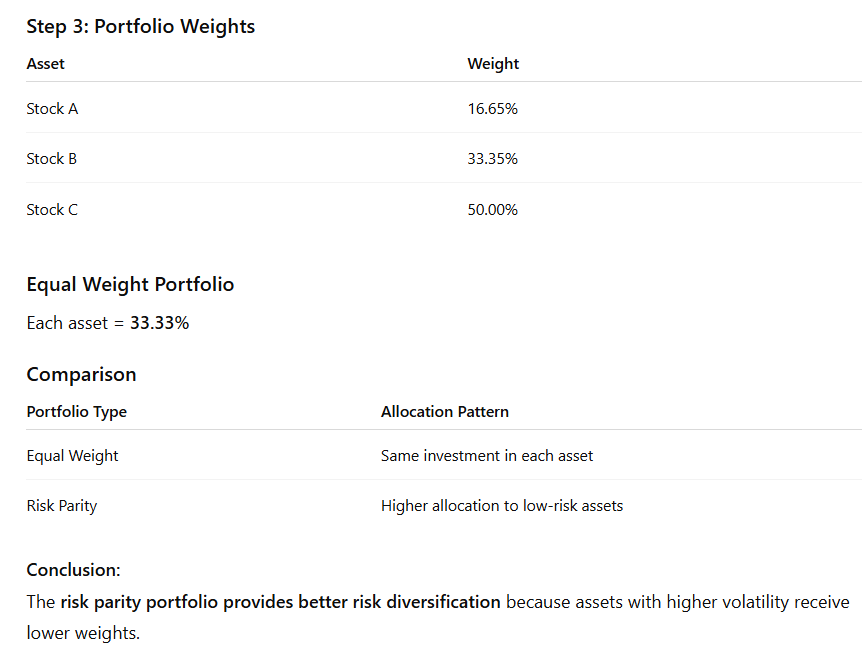
\includegraphics{figures/fig_0042.png}
\textgreater{} OCR cue: Step 3: Portfolio Weights Asset Weight Stock A
16.65\% Stock B 33.35\% Stock C 50.00\% Equal Weight Portfolio Each
asset = 33.33\% Comparison Portfolio Type Allocation Pattern Equal
Weight 'Same investment in each asset Risk Parity Higher allocation to
low-risk assets Conclusion: The risk parity portfolio provides better
risk diversification because assets with higher volatility receive lower
weights.

\hypertarget{unit-47-full-risk-parity-portfolios.pptx}{%
\subsection{UNIT 4/7 Full Risk Parity
Portfolios.pptx}\label{unit-47-full-risk-parity-portfolios.pptx}}

\hypertarget{figure-1-slide-9}{%
\subsubsection{Figure 1 (Slide 9)}\label{figure-1-slide-9}}

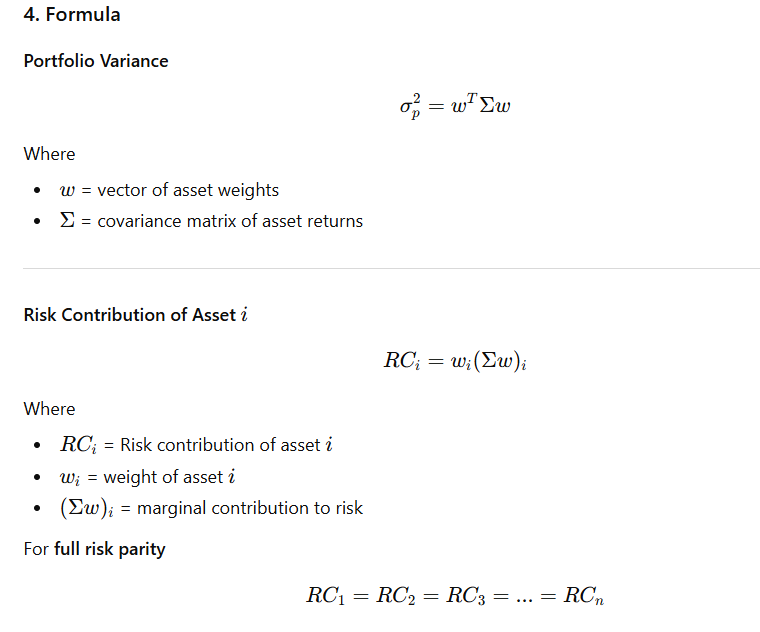
\includegraphics{figures/fig_0043.png}
\textgreater{} OCR cue: 4, Formula Portfolio Variance o =w' dw Where *
w= vector of asset weights « = covariance matrix of asset returns Risk
Contribution of Asset 7 RC; = w;(Zw); Where * RC; = Risk contribution of
asset i * w; = weight of asset i « (Zw); = marginal contribution to risk
For full risk parity RC, = RCz = RC3 =\ldots{} = RC,

\hypertarget{figure-2-slide-10}{%
\subsubsection{Figure 2 (Slide 10)}\label{figure-2-slide-10}}

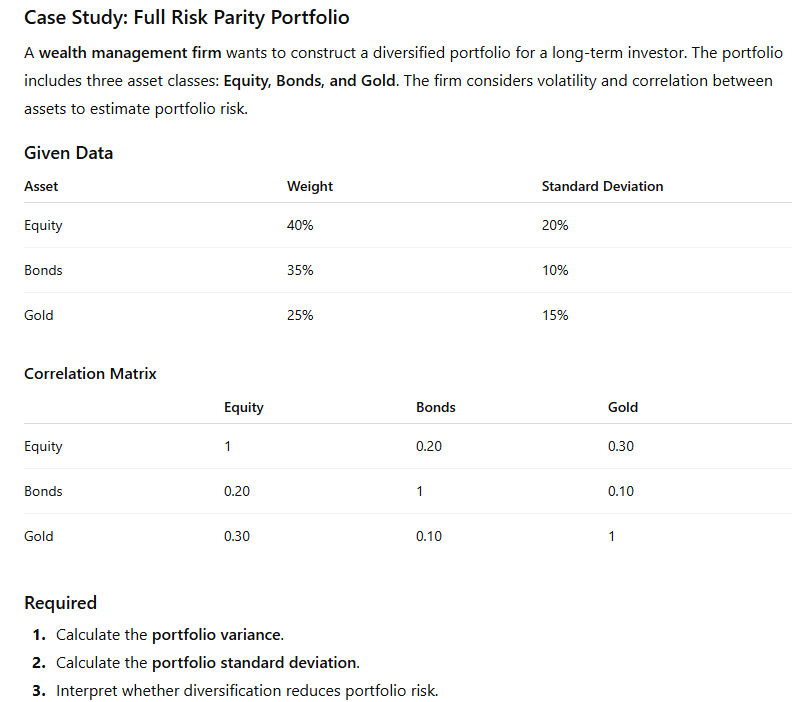
\includegraphics{figures/fig_0044.png}
\textgreater{} OCR cue: Case Study: Full Risk Parity Portfolio A.wealth
management firm wants to construct a diversified portfolio for a
long-term investor. The portfolio includes three asset classes: Equity,
Bonds, and Gold. The firm considers volatility and correlation between
assets to estimate portfolio risk. en Data Asset Equity Bonds Gold
Correlation Matrix Equity Equity 1 Bonds 0.20 Gold 030 Required 1.
Calculate

\hypertarget{figure-3-slide-11}{%
\subsubsection{Figure 3 (Slide 11)}\label{figure-3-slide-11}}

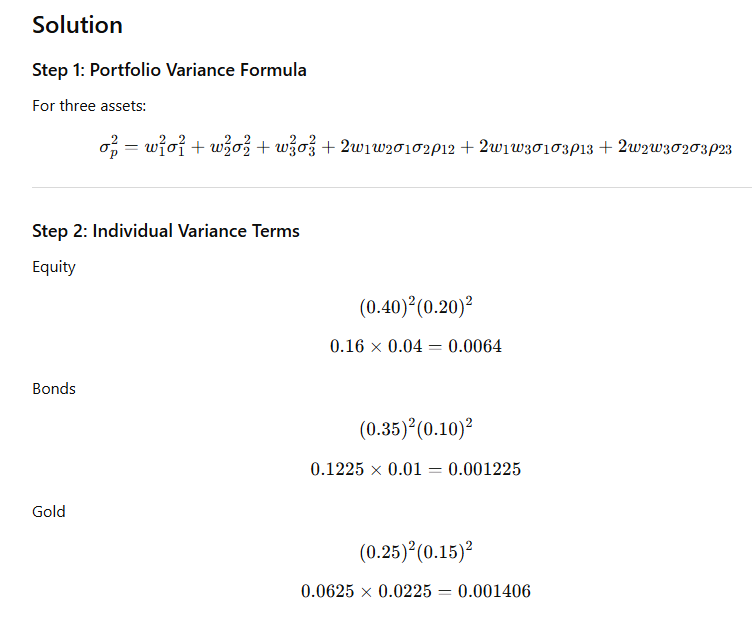
\includegraphics{figures/fig_0045.png}
\textgreater{} OCR cue: Solution Step 1: Portfolio Variance Formula For
three assets: 252. wo2 + w? oO, = wyoj + w303 + w30\% + Qwiweoid2p12 +
2wiwso103pi3 + 2w2w30203p23 Step 2: Individual Variance Terms Equity
(0.40)?(0.20) 0.16 x 0.04 = 0.0064 Bonds (0.35)?(0.10) 0.1225 x 0.01 =
0.001225 Gold (0.25)°(0.15)? 0.0625 x 0.0225 = 0.001406

\hypertarget{figure-4-slide-12}{%
\subsubsection{Figure 4 (Slide 12)}\label{figure-4-slide-12}}

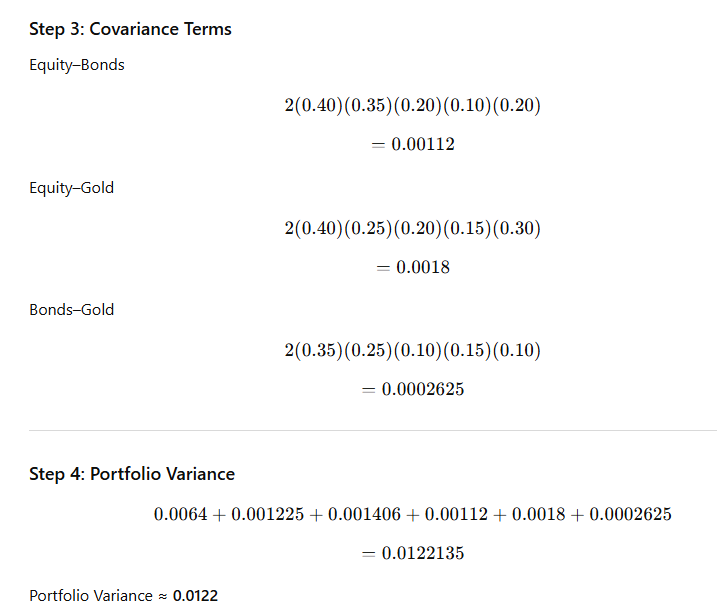
\includegraphics{figures/fig_0046.png}
\textgreater{} OCR cue: Step 3: Covariance Terms Equity-Bonds
2(0.40)(0.35) (0.20)(0.10) (0.20) = 0.00112 Equity-Gold 2(0.40)(0.25)
(0.20)(0.15) (0.30) = 0.0018 Bonds-Gold 2(0.35)(0.25)(0.10)(0.15)(0.10)
= 0.0002625 Step 4: Portfolio Variance 0.0064 + 0.001225 + 0.001406 +
0.00112 + 0.0018 + 0.0002625 = 0.0122135 Portfolio Variance = 0.0122

\hypertarget{figure-5-slide-13}{%
\subsubsection{Figure 5 (Slide 13)}\label{figure-5-slide-13}}

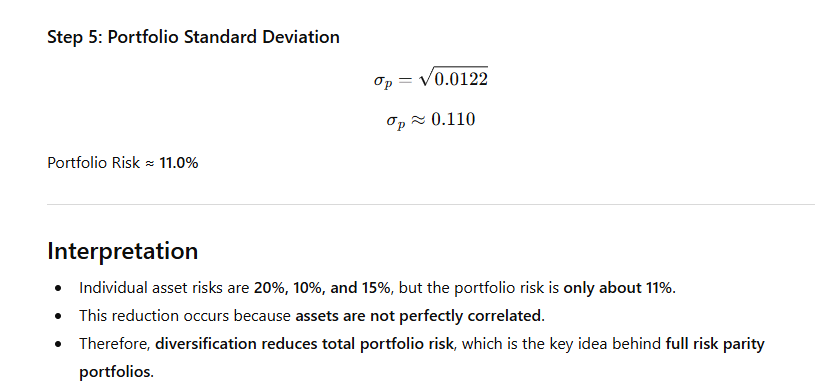
\includegraphics{figures/fig_0047.png}
\textgreater{} OCR cue: Step 5: Portfolio Standard Deviation op =
V0.0122 op © 0.110 Portfolio Risk = 11.0\% Interpretation Individual
asset risks are 20\%, 10\%, and 15\%, but the portfolio risk is only
about 11\%. © This reduction occurs because assets are not perfectly
correlated. Therefore, diversification reduces total portfolio risk,
which is the key idea behind full risk parity portfolios.

\hypertarget{figure-6-slide-14}{%
\subsubsection{Figure 6 (Slide 14)}\label{figure-6-slide-14}}

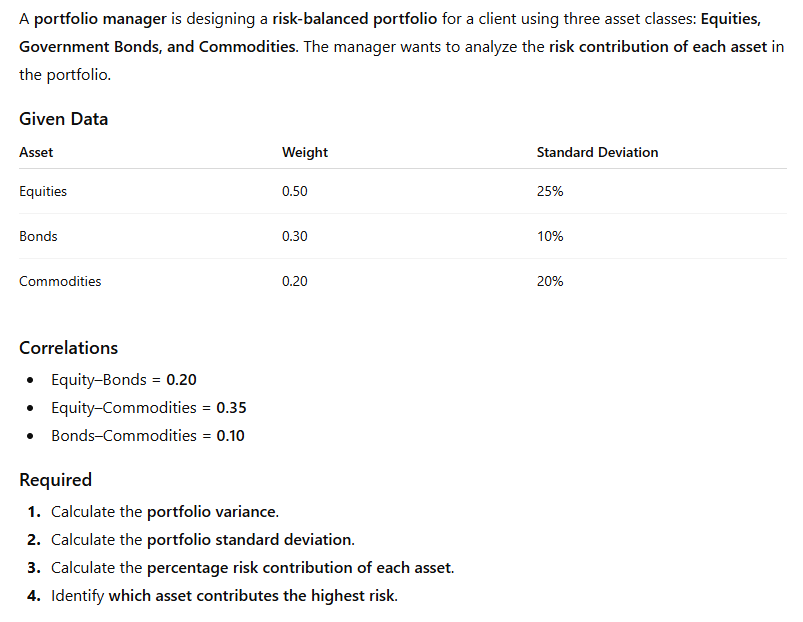
\includegraphics{figures/fig_0048.png}
\textgreater{} OCR cue: A portfolio manager is designing a risk-balanced
portfolio for a client using three asset classes: Equities, Government
Bonds, and Commodities. The manager wants to analyze the risk
contribution of each asset in the portfolio. Given Data Asset Weight
Standard Deviation Equities 0.50 25\% Bonds 0.30 10\% Commodities 0.20
20\% Correlations © Equity-Bonds = 0.20 © Equity-Commodities = 0.35 ©
Bonds-Commo

\hypertarget{figure-7-slide-15}{%
\subsubsection{Figure 7 (Slide 15)}\label{figure-7-slide-15}}

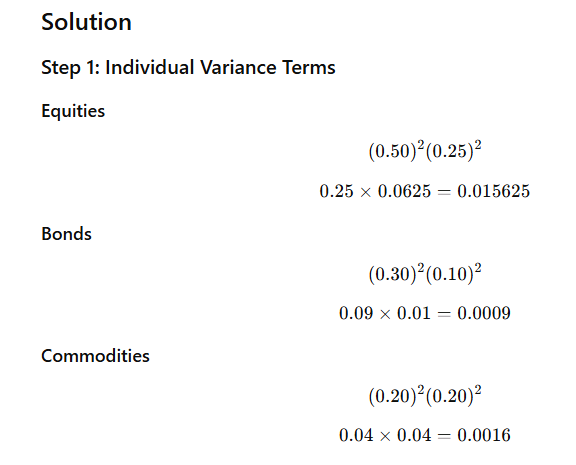
\includegraphics{figures/fig_0049.png}
\textgreater{} OCR cue: Solution Step 1: Individual Variance Terms
Equities (0.50)?(0.25) 0.25 x 0.0625 --- 0.015625 Bonds (0.30)?(0.10)
0.09 x 0.01 = 0.0009 Commodities (0.20)?(0.20) 0.04 x 0.04 = 0.0016

\hypertarget{figure-8-slide-16}{%
\subsubsection{Figure 8 (Slide 16)}\label{figure-8-slide-16}}

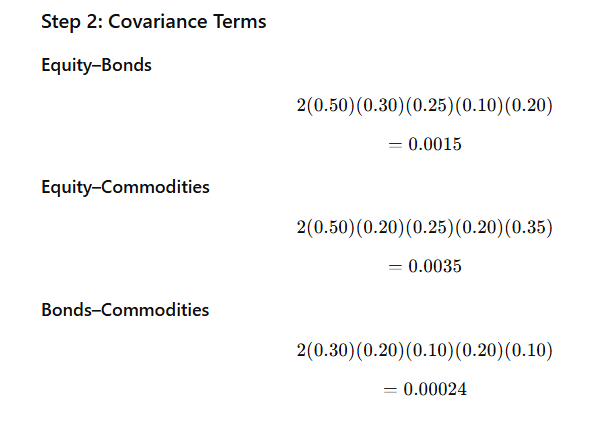
\includegraphics{figures/fig_0050.png}
\textgreater{} OCR cue: Step 2: Covariance Terms Equity-Bonds 2(0.50)
(0.30)(0.25)(0.10)(0.20) = 0.0015 Equity-Commodities 2(0.50) (0.20)
(0.25) (0.20)(0.35) = 0.0035 Bonds-Commodities
2(0.30)(0.20)(0.10)(0.20)(0.10) = 0.00024

\hypertarget{figure-9-slide-17}{%
\subsubsection{Figure 9 (Slide 17)}\label{figure-9-slide-17}}

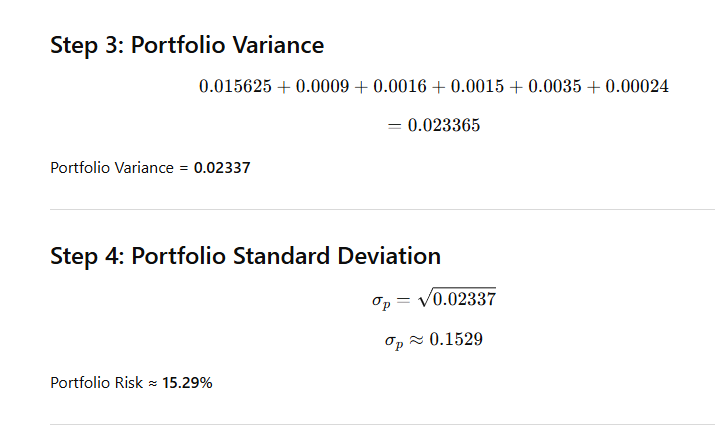
\includegraphics{figures/fig_0051.png}
\textgreater{} OCR cue: Step 3: Portfolio Variance 0.015625 + 0.0009 +
0.0016 + 0.0015 + 0.0035 + 0.00024 = 0.023365 Portfolio Variance =
0.02337 Step 4: Portfolio Standard Deviation oy = V0.02337 op © 0.1529
Portfolio Risk = 15.29\%

\hypertarget{figure-10-slide-18}{%
\subsubsection{Figure 10 (Slide 18)}\label{figure-10-slide-18}}

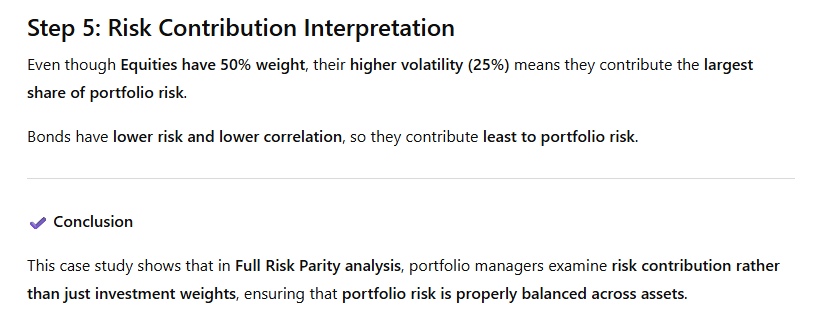
\includegraphics{figures/fig_0052.png}
\textgreater{} OCR cue: Step 5: Risk Contribution Interpretation Even
though Equities have 50\% weight, their higher volatility (25\%) means
they contribute the largest share of portfolio risk. Bonds have lower
risk and lower correlation, so they contribute least to portfolio risk.
¥ Conclusion This case study shows that in Full Risk Parity analysis,
portfolio managers examine risk contribution rather than just investment

\hypertarget{unit-48-shrinkage-estimators.pptx}{%
\subsection{UNIT 4/8 Shrinkage
Estimators.pptx}\label{unit-48-shrinkage-estimators.pptx}}

\hypertarget{figure-1-slide-12}{%
\subsubsection{Figure 1 (Slide 12)}\label{figure-1-slide-12}}

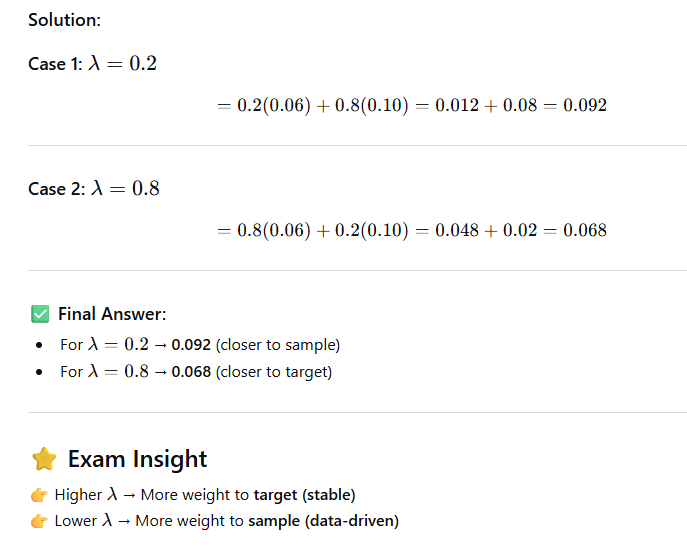
\includegraphics{figures/fig_0053.png}
\textgreater{} OCR cue: Solution: Case 1: A = 0.2 = 0.2(0.06) +
0.8(0.10) = 0.012 + 0.08 = 0.092 Case 2: A = 0.8 = 0.8(0.06) + 0.2(0.10)
= 0.048 + 0.02 = 0.068 Final Answer: © For A = 0.2 = 0.092 (closer to
sample) © For A = 0.8 --- 0.068 (closer to target) ww Exam Insight ©
Higher ~+ More weight to target (stable) \& Lower ~+ More weight to
sample (data-driven)

\hypertarget{figure-2-slide-14}{%
\subsubsection{Figure 2 (Slide 14)}\label{figure-2-slide-14}}

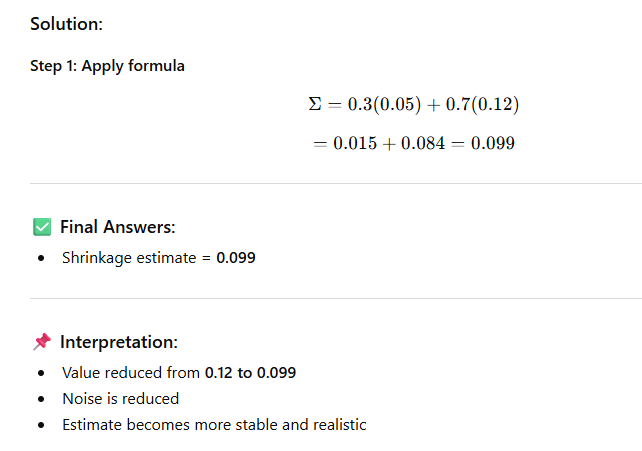
\includegraphics{figures/fig_0054.png}
\textgreater{} OCR cue: Solution: Step 1: Apply formula B = 0.3(0.05) +
0.7(0.12) = 0.015 + 0.084 = 0.099 Final Answers: * Shrinkage estimate =
0.099 \% Interpretatio © Value reduced from 0.12 to 0.099 * Noise is
reduced * Estimate becomes more stable and realistic

\hypertarget{figure-3-slide-15}{%
\subsubsection{Figure 3 (Slide 15)}\label{figure-3-slide-15}}

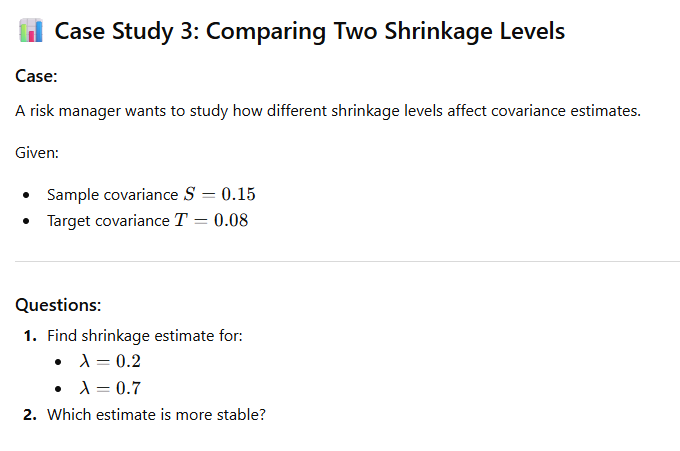
\includegraphics{figures/fig_0055.png}
\textgreater{} OCR cue: il Case Study 3: Comparing Two Shrinkage Levels
Case: A risk manager wants to study how different shrinkage levels
affect covariance estimates. Given: © Sample covariance \$ = 0.15 ©
Target covariance T = 0.08 Questions: 1. Find shrinkage estimate for: °
A=0.2 ° A=0.7 2. Which estimate is more stable?

\hypertarget{figure-4-slide-16-1}{%
\subsubsection{Figure 4 (Slide 16)}\label{figure-4-slide-16-1}}

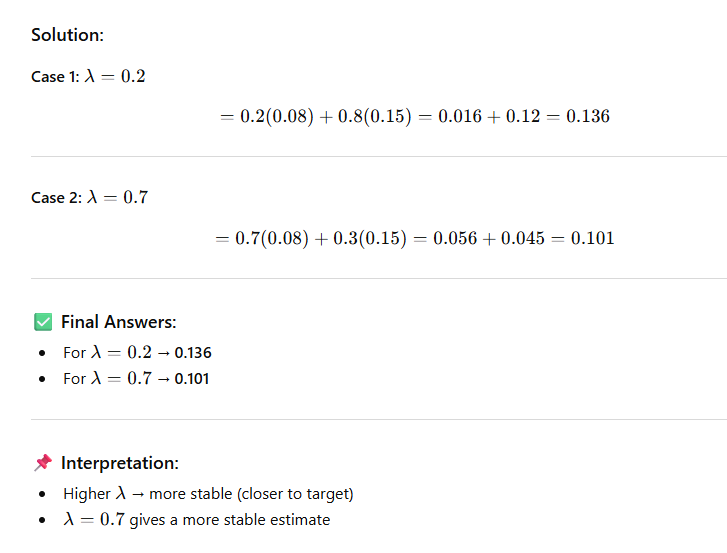
\includegraphics{figures/fig_0056.png}
\textgreater{} OCR cue: Solution: Case 1: ~= 0.2 = 0.2(0.08) + 0.8(0.15)
= 0.016 + 0.12 = 0.136 Case 2: = 0.7 = 0.7(0.08) + 0.3(0.15) = 0.056 +
0.045 = 0.101 Final Answers: © ForA = 0.2 + 0.136 ¢ ForA = 0.7 + 0.101
\% Interpretation: * Higher A --- more stable (closer to target) * 2
=0.7 gives a more stable estimate

\hypertarget{unit-49-ewma-exponentially-weighted-moving-average.pptx}{%
\subsection{UNIT 4/9 EWMA (Exponentially Weighted Moving
Average).pptx}\label{unit-49-ewma-exponentially-weighted-moving-average.pptx}}

\hypertarget{figure-1-slide-3-1}{%
\subsubsection{Figure 1 (Slide 3)}\label{figure-1-slide-3-1}}

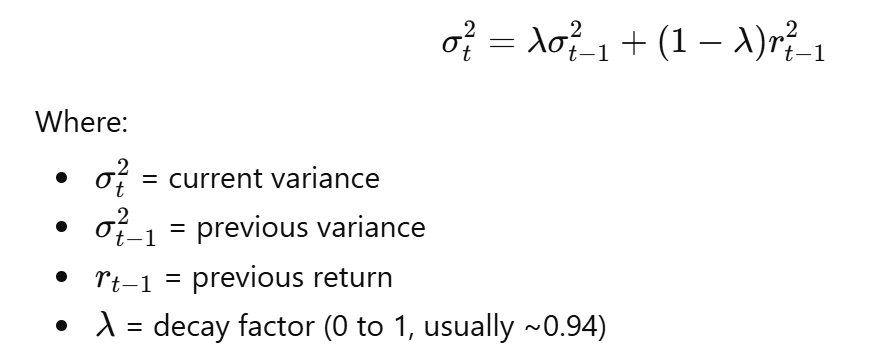
\includegraphics{figures/fig_0057.png}
\textgreater{} OCR cue: of = op +(1--- Area © of; = current variance ©
O;\_, = previous variance © Tt---1 = previous return e = decay factor (0
to 1, usually \textasciitilde0.94)

\hypertarget{figure-2-slide-5}{%
\subsubsection{Figure 2 (Slide 5)}\label{figure-2-slide-5}}

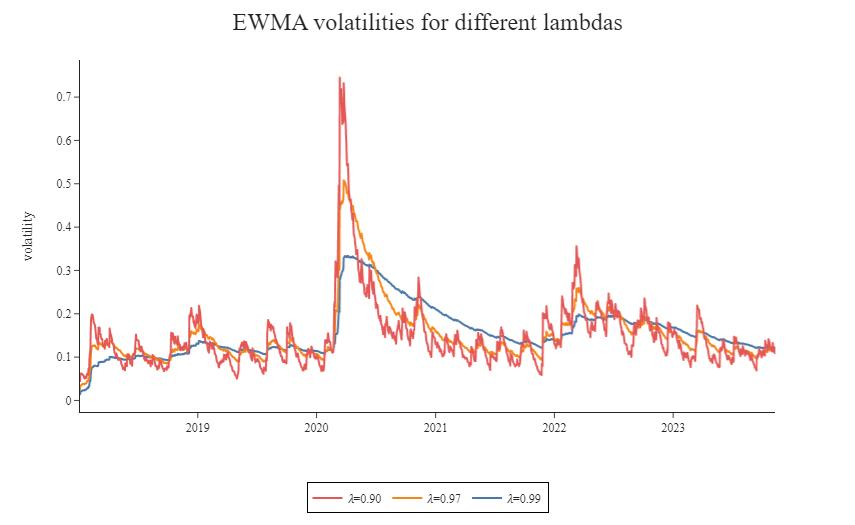
\includegraphics{figures/fig_0058.png}
\textgreater{} OCR cue: volatility EWMA volatilities for different
lambdas 2019 2020 2021 2022 2023 --- 7099 --- 1-091 --- 1-099

\hypertarget{figure-3-slide-6}{%
\subsubsection{Figure 3 (Slide 6)}\label{figure-3-slide-6}}

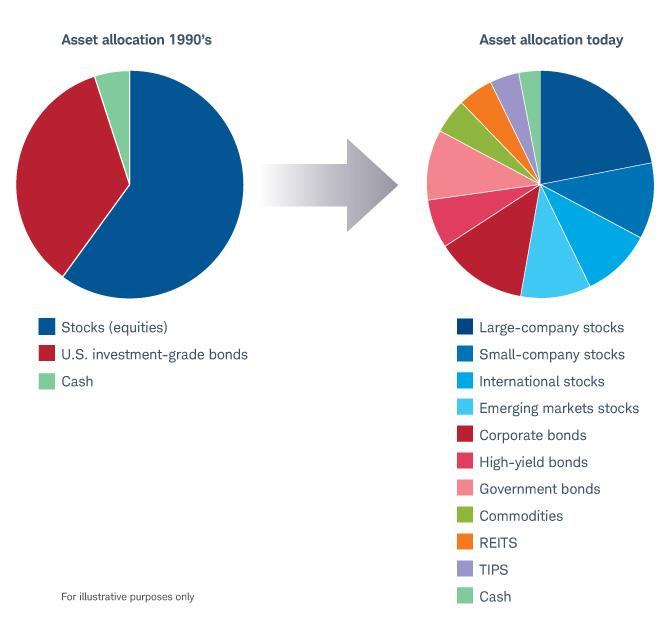
\includegraphics{figures/fig_0059.png}
\textgreater{} OCR cue: Asset allocation 1990's Asset allocation today
Hl Stocks (equities) U.S. investment-grade bonds i Cash For ilustrative
purposes only I Large-company stocks I Small-company stocks i
international stocks 1 Emerging markets stocks i Corporate bonds Wi
High-yield bonds Il Government bonds I Commodities Wrens its I cash

\hypertarget{figure-4-slide-13}{%
\subsubsection{Figure 4 (Slide 13)}\label{figure-4-slide-13}}

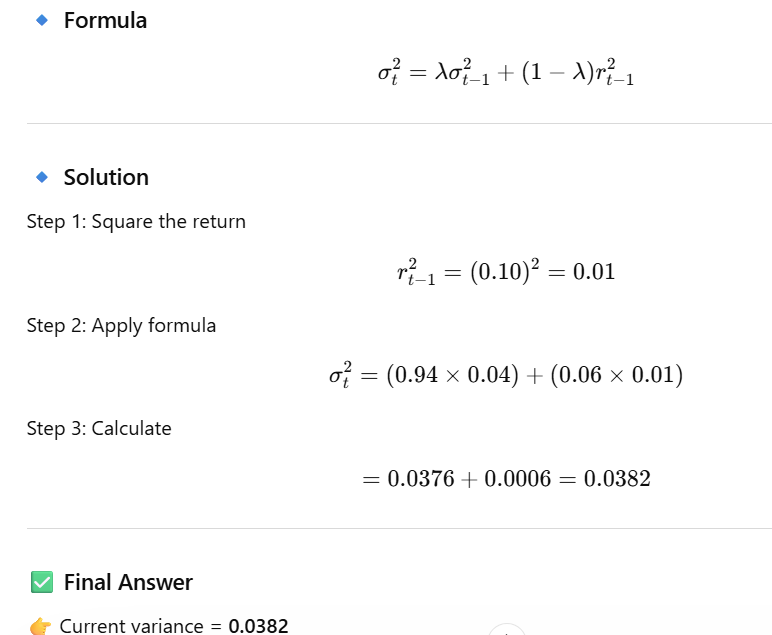
\includegraphics{figures/fig_0060.png}
\textgreater{} OCR cue: ¢@ Formula of = dopey + (L---A)rz4 * Solution
Step 1: Square the return r?\_, = (0.10)? = 0.01 Step 2: Apply formula
oa; = (0.94 x 0.04) + (0.06 x 0.01) Step 3: Calculate = 0.0376 + 0.0006
= 0.0382 Final Answer © Current variance = 0.0382

\hypertarget{figure-5-slide-15-2}{%
\subsubsection{Figure 5 (Slide 15)}\label{figure-5-slide-15-2}}

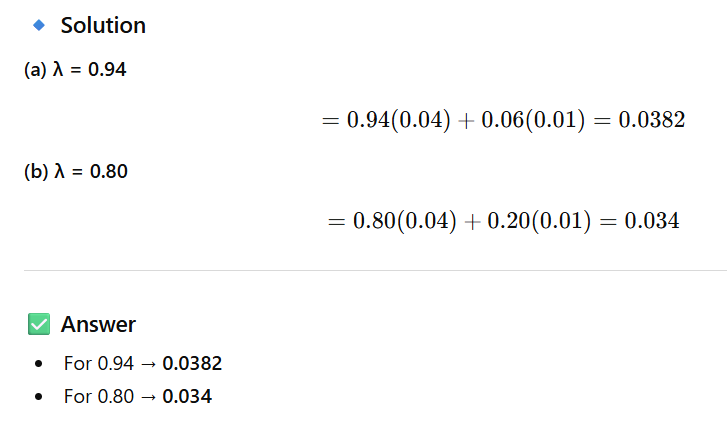
\includegraphics{figures/fig_0061.png}
\textgreater{} OCR cue: * Solution (a) A = 0.94 = 0.94(0.04) +
0.06(0.01) = 0.0382 (b) A = 0.80 = 0.80(0.04) + 0.20(0.01) = 0.034
Answer © For 0.94 --- 0.0382 © For 0.80 --- 0.034

\hypertarget{figure-6-slide-17}{%
\subsubsection{Figure 6 (Slide 17)}\label{figure-6-slide-17}}

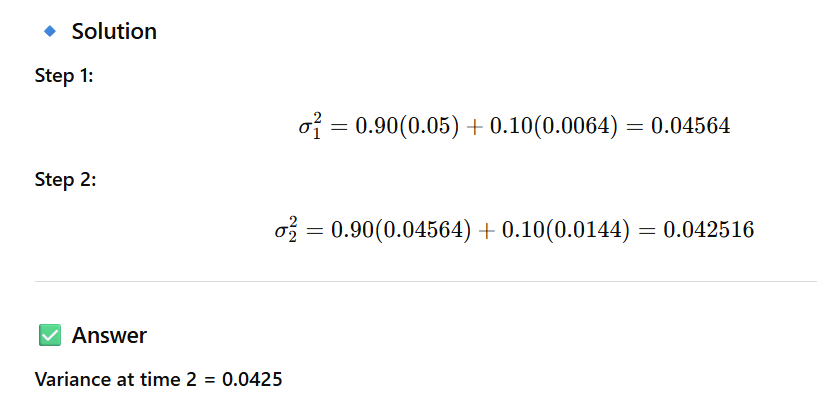
\includegraphics{figures/fig_0062.png}
\textgreater{} OCR cue: * Solution Step 1: a\} = 0.90(0.05) +
0.10(0.0064) = 0.04564 Step 2: o3 = 0.90(0.04564) + 0.10(0.0144) =
0.042516 Answer Variance at time 2 = 0.0425

\hypertarget{figure-7-slide-19-1}{%
\subsubsection{Figure 7 (Slide 19)}\label{figure-7-slide-19-1}}

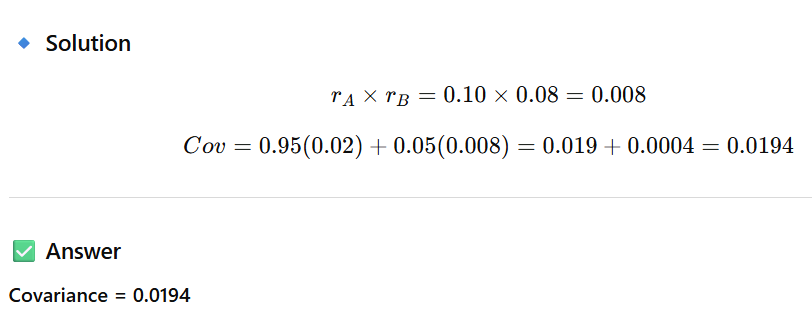
\includegraphics{figures/fig_0063.png}
\textgreater{} OCR cue: * Solution ra X rz = 0.10 x 0.08 = 0.008 Cov =
0.95(0.02) + 0.05(0.008) = 0.019 + 0.0004 = 0.0194 Answer Covariance =
0.0194

\hypertarget{figure-8-slide-22}{%
\subsubsection{Figure 8 (Slide 22)}\label{figure-8-slide-22}}

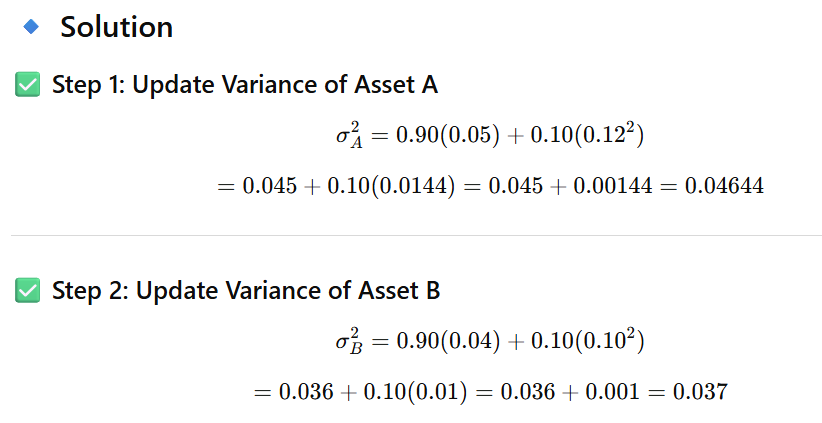
\includegraphics{figures/fig_0064.png}
\textgreater{} OCR cue: ¢ Solution Step 1: Update Variance of Asset A o,
= 0.90(0.05) + 0.10(0.12'') = 0.045 + 0.10(0.0144) = 0.045 + 0.00144 =
0.04644 Step 2: Update Variance of Asset B o\% = 0.90(0.04) +
0.10(0.107) = 0.036 + 0.10(0.01) = 0.036 + 0.001 = 0.037

\hypertarget{figure-9-slide-23}{%
\subsubsection{Figure 9 (Slide 23)}\label{figure-9-slide-23}}

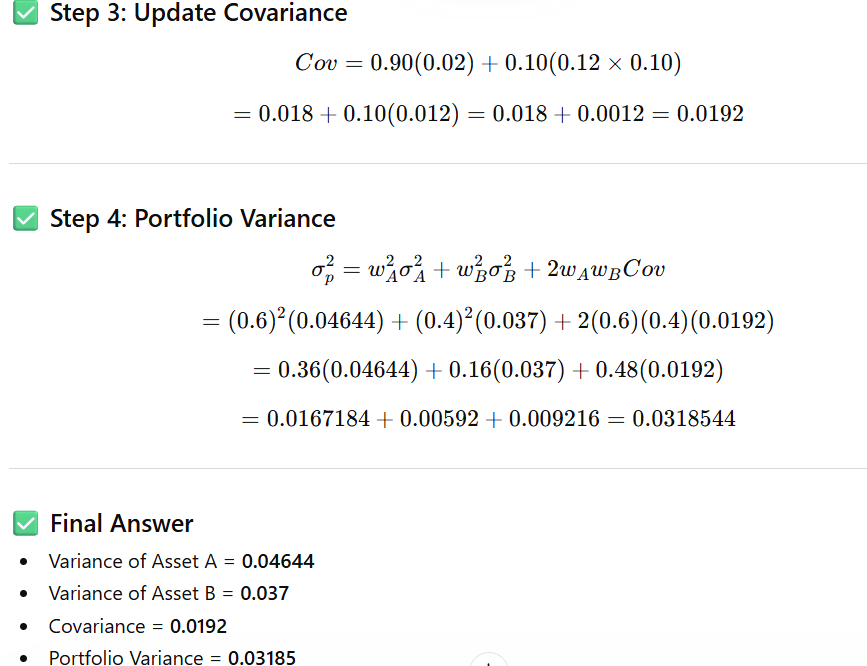
\includegraphics{figures/fig_0065.png}
\textgreater{} OCR cue: Step 3: Update Covariance Cov = 0.90(0.02) +
0.10(0.12 x 0.10) = 0.018 + 0.10(0.012) = 0.018 + 0.0012 = 0.0192 Step
4: Portfolio Variance oO, = we, + WRoR + 2WawgCov = (0.6)?(0.04644) +
(0.4)?(0.037) + 2(0.6)(0.4) (0.0192) = 0.36(0.04644) + 0.16(0.037) +
0.48(0.0192) = 0.0167184 + 0.00592 + 0.009216 = 0.0318544 Final Answer
Variance of Asset A = 0.04644 Variance of Asset B = 0.037 Covariance =
0.0

\hypertarget{unit-52-cppi.pptx}{%
\subsection{UNIT 5/2 CPPI.pptx}\label{unit-52-cppi.pptx}}

\hypertarget{figure-1-slide-1-1}{%
\subsubsection{Figure 1 (Slide 1)}\label{figure-1-slide-1-1}}

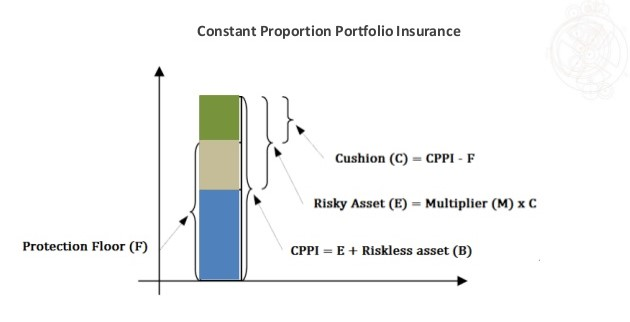
\includegraphics{figures/fig_0066.jpg} \textgreater{} OCR
cue: Constant Proportion Portfolio Insurance h » Cushion (C) = CPPI- F »
Risky Asset (E) = Multiplier (M) x C Protection Floor (F) CPPI = E +
Riskless asset (B) \textgreater{}

\hypertarget{figure-2-slide-3}{%
\subsubsection{Figure 2 (Slide 3)}\label{figure-2-slide-3}}

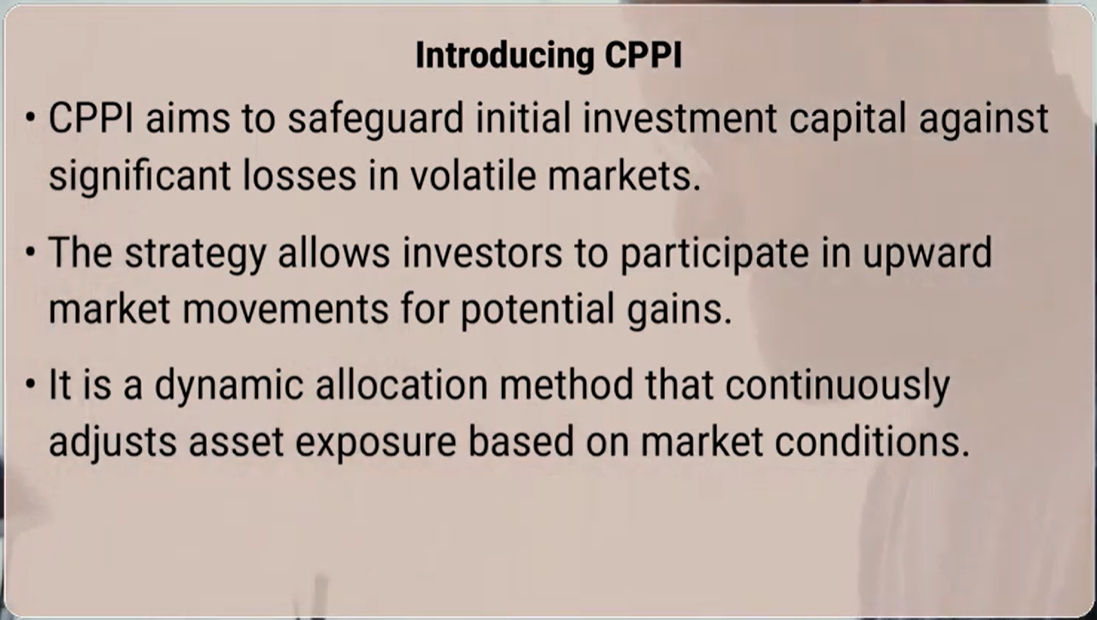
\includegraphics{figures/fig_0067.png} \textgreater{} OCR
cue: Introducing CPPI * CPPI aims to safeguard initial investment
capital against significant losses in volatile markets. * The strategy
allows investors to participate in upward market movements for potential
gains. * It is a dynamic allocation method that continuously adjusts
asset exposure based on market conditions.

\hypertarget{figure-3-slide-6-1}{%
\subsubsection{Figure 3 (Slide 6)}\label{figure-3-slide-6-1}}

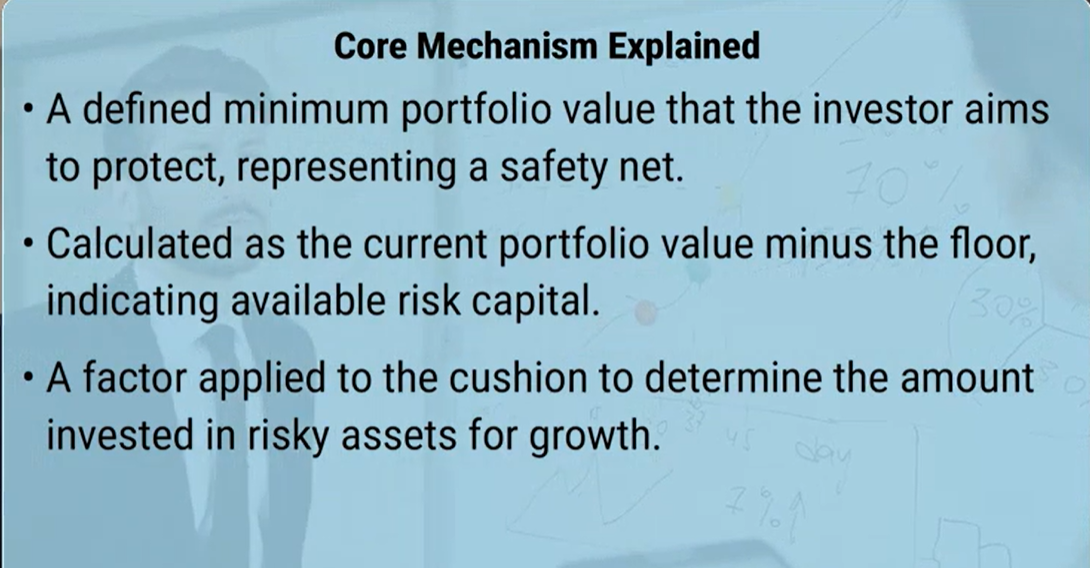
\includegraphics{figures/fig_0068.png} \textgreater{} OCR
cue: Core Mechanism Explained * A defined minimum portfolio value that
the investor aims to protect, representing a safety net. * Calculated as
the current portfolio value minus the floor, indicating available risk
capital. - A factor applied to the cushion to determine the amount
invested in risky assets for growth.

\hypertarget{figure-4-slide-7}{%
\subsubsection{Figure 4 (Slide 7)}\label{figure-4-slide-7}}

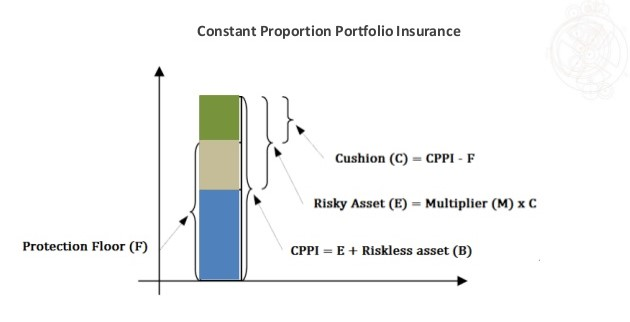
\includegraphics{figures/fig_0069.jpg} \textgreater{} OCR
cue: Constant Proportion Portfolio Insurance h » Cushion (C) = CPPI- F »
Risky Asset (E) = Multiplier (M) x C Protection Floor (F) CPPI = E +
Riskless asset (B) \textgreater{}

\hypertarget{unit-53-analysis-simulating-cppi-using-gbm-monte-carlo-evaluation-analyzing-performance-drawdowns-floor-violations-designing-and-calibrating-cppi-strategies-light-conceptual.pptx}{%
\subsection{\texorpdfstring{UNIT 5/\emph{3 Analysis} Simulating CPPI
using GBM, Monte Carlo evaluation, Analyzing performance, drawdowns,
floor violations, Designing and calibrating CPPI strategies (light,
conceptual).pptx}{UNIT 5/3 Analysis Simulating CPPI using GBM, Monte Carlo evaluation, Analyzing performance, drawdowns, floor violations, Designing and calibrating CPPI strategies (light, conceptual).pptx}}\label{unit-53-analysis-simulating-cppi-using-gbm-monte-carlo-evaluation-analyzing-performance-drawdowns-floor-violations-designing-and-calibrating-cppi-strategies-light-conceptual.pptx}}

\hypertarget{figure-1-slide-7-2}{%
\subsubsection{Figure 1 (Slide 7)}\label{figure-1-slide-7-2}}

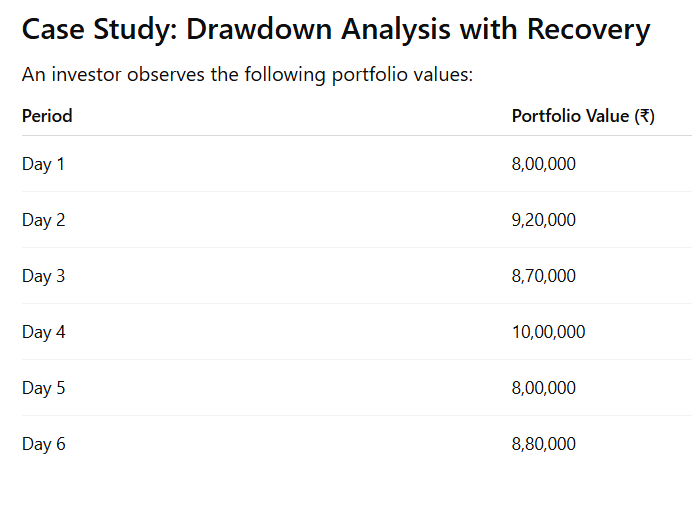
\includegraphics{figures/fig_0070.png}
\textgreater{} OCR cue: Case Study: Drawdown Analysis with Recovery An
investor observes the following portfolio values: Period Portfolio Value
(3) Day 1 8,00,000 Day 2 9,20,000 Day 3 8,70,000 Day 4 10,00,000 Day 5
8,00,000 Day 6 8,80,000

\hypertarget{figure-2-slide-8-1}{%
\subsubsection{Figure 2 (Slide 8)}\label{figure-2-slide-8-1}}

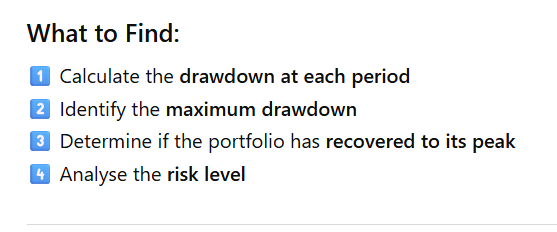
\includegraphics{figures/fig_0071.png}
\textgreater{} OCR cue: What to Find: @ Calculate the drawdown at each
period G Identify the maximum drawdown © Determine if the portfolio has
recovered to its peak Analyse the risk level

\hypertarget{figure-3-slide-9-1}{%
\subsubsection{Figure 3 (Slide 9)}\label{figure-3-slide-9-1}}

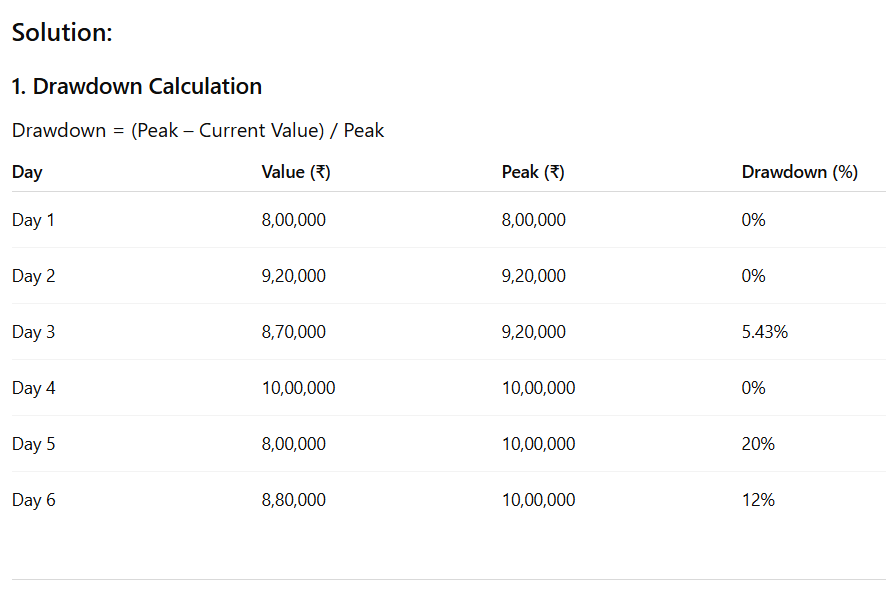
\includegraphics{figures/fig_0072.png}
\textgreater{} OCR cue: Solution: 1. Drawdown Calculation Drawdown =
(Peak --- Current Value) / Peak Day Value (3) Peak (3) Drawdown (\%) Day
1 8,00,000 8,00,000 0\% Day 2 9,20,000 9,20,000 0\% Day 3 8,70,000
9,20,000 543\% Day 4 10,00,000 10,00,000 0\% Day 5 8,00,000 10,00,000
20\% Day 6 8,80,000 10,00,000 12\%

\hypertarget{figure-4-slide-10-1}{%
\subsubsection{Figure 4 (Slide 10)}\label{figure-4-slide-10-1}}

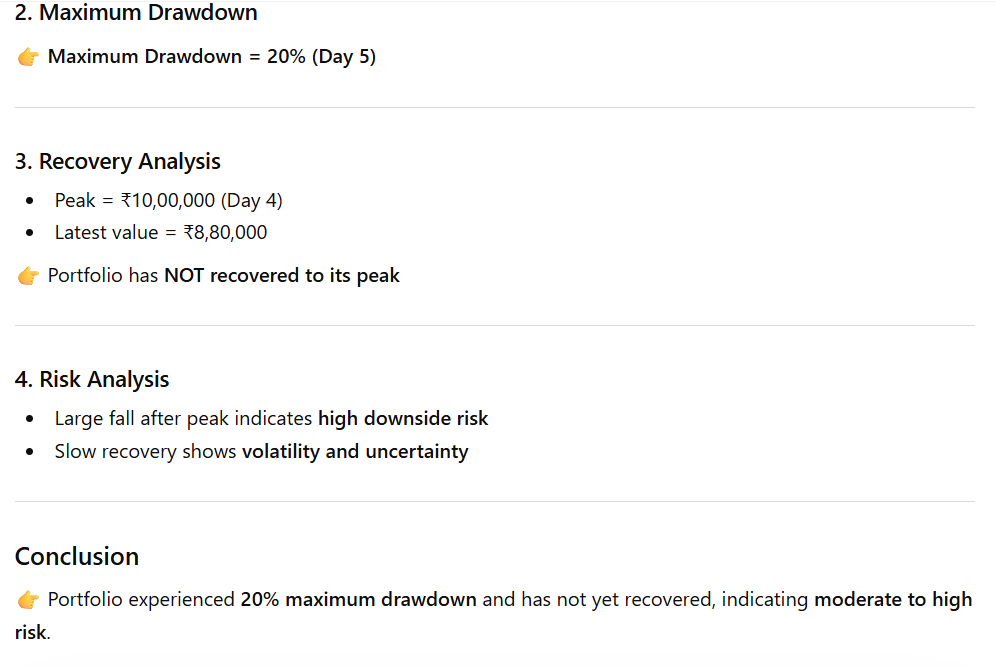
\includegraphics{figures/fig_0073.png}
\textgreater{} OCR cue: 2. Maximum Drawdown «© Maximum Drawdown = 20\%
(Day 5) 3. Recovery Analysis © Peak = \%10,00,000 (Day 4) e Latest value
= \%8,80,000 \& Portfolio has NOT recovered to its peak 4. Risk Analysis
¢ Large fall after peak indicates high downside risk © Slow recovery
shows volatility and uncertainty Conclusion © Portfolio experienced 20\%
maximum drawdown and has not yet recovered, indicating moderate to hig

\hypertarget{figure-5-slide-17-1}{%
\subsubsection{Figure 5 (Slide 17)}\label{figure-5-slide-17-1}}

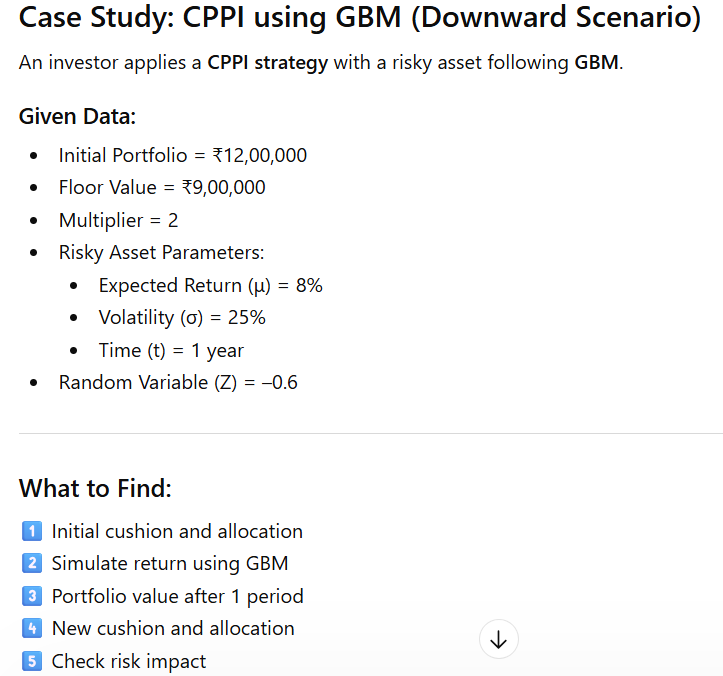
\includegraphics{figures/fig_0074.png}
\textgreater{} OCR cue: Case Study: CPPI using GBM (Downward Scenario)
An investor applies a CPPI strategy with a risky asset following GBM.
Given Data: Initial Portfolio = \%12,00,000 Floor Value = \%9,00,000
Multiplier = 2 Risky Asset Parameters: © Expected Return (yu) = 8\% ©
Volatility (6) = 25\% © Time (t) = 1 year Random Variable (Z) = -0.6
What to Find: @ Initial cushion and allocation G Simulate return using
GBM © Po

\hypertarget{figure-6-slide-18-1}{%
\subsubsection{Figure 6 (Slide 18)}\label{figure-6-slide-18-1}}

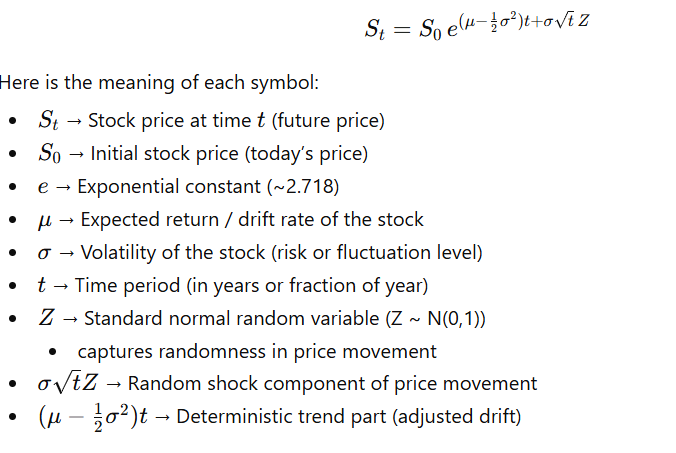
\includegraphics{figures/fig_0075.png}
\textgreater{} OCR cue: S: = So elt gar trovt Z Here is the meaning of
each symbol: Si --- Stock price at time t (future price) So = Initial
stock price (today's price) e --- Exponential constant
(\textasciitilde2.718) \}. \textasciitilde{} Expected return / drift
rate of the stock o = Volatility of the stock (risk or fluctuation
level) t --- Time period (in years or fraction of year) Z = Standard
normal random variable (Z \textasciitilde{} N(0,1)) © captures
randomness in

\hypertarget{figure-7-slide-19-2}{%
\subsubsection{Figure 7 (Slide 19)}\label{figure-7-slide-19-2}}

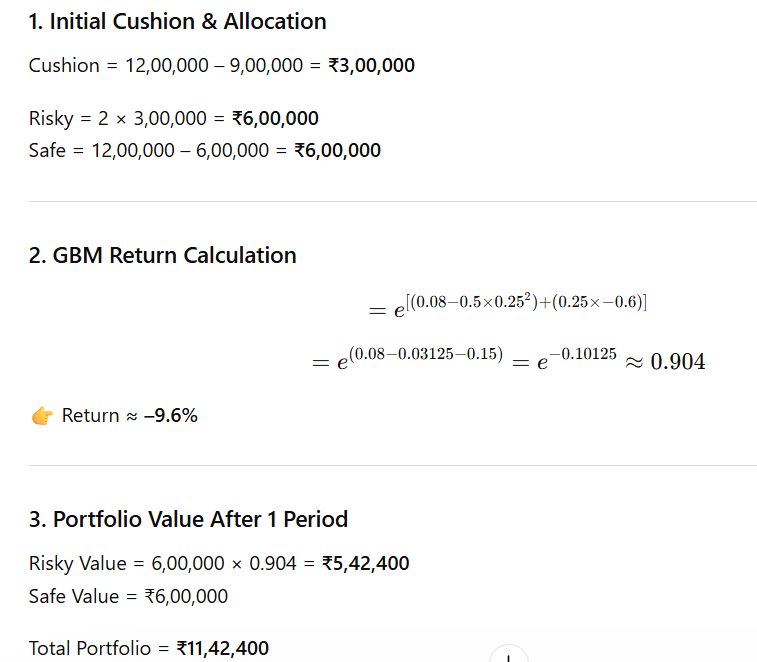
\includegraphics{figures/fig_0076.png}
\textgreater{} OCR cue: 1. Initial Cushion \& Allocation Cushion =
12,00,000 --- 9,00,000 = \%3,00,000 Risky = 2 x 3,00,000 = \%6,00,000
Safe = 12,00,000 --- 6,00,000 = \%6,00,000 2. GBM Return Calculation =
el(0.08-0.5x0.25'') +(0.25x---0.6){]} = e(0-08-0.03125-0.15) \_
¢-0.10125 \textasciitilde{} 9.994 © Return = -9.6\% 3. Portfolio Value
After 1 Period Risky Value = 6,00,000 x 0.904 = 5,42,400 Safe Value =
\%6,00,000 Total Portfolio = \%11,42,400

\hypertarget{figure-8-slide-20-1}{%
\subsubsection{Figure 8 (Slide 20)}\label{figure-8-slide-20-1}}

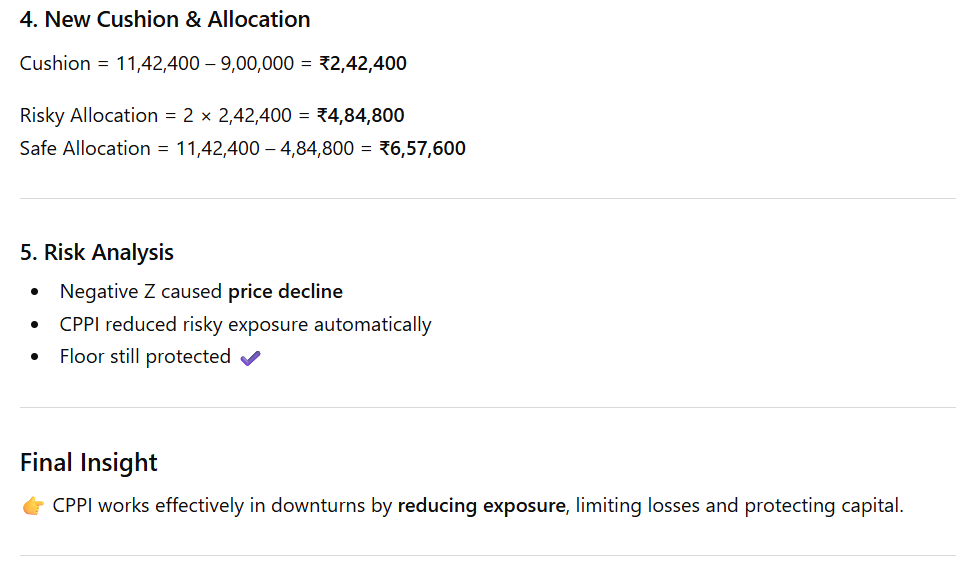
\includegraphics{figures/fig_0077.png}
\textgreater{} OCR cue: 4. New Cushion \& Allocation Cushion = 11,42,400
--- 9,00,000 = 2,42,400 Risky Allocation = 2 x 2,42,400 = \%4,84,800
Safe Allocation = 11,42,400 --- 4,84,800 = 6,57,600 5. Risk Analysis ¢
Negative Z caused price decline © CPPI reduced risky exposure
automatically © Floor still protected 4 Final Insight © CPPI works
effectively in downturns by reducing exposure, limiting losses and
protecting capital.

\hypertarget{unit-61-portfolio-revision.ppt}{%
\subsection{UNIT 6/1 Portfolio
revision.ppt}\label{unit-61-portfolio-revision.ppt}}

\hypertarget{figure-1-page-1}{%
\subsubsection{Figure 1 (Page 1)}\label{figure-1-page-1}}


\includegraphics{figures/fig_0078.png}
\textgreater{} OCR cue: Chapter 21 Portfolio Revision

\hypertarget{figure-2-page-2}{%
\subsubsection{Figure 2 (Page 2)}\label{figure-2-page-2}}

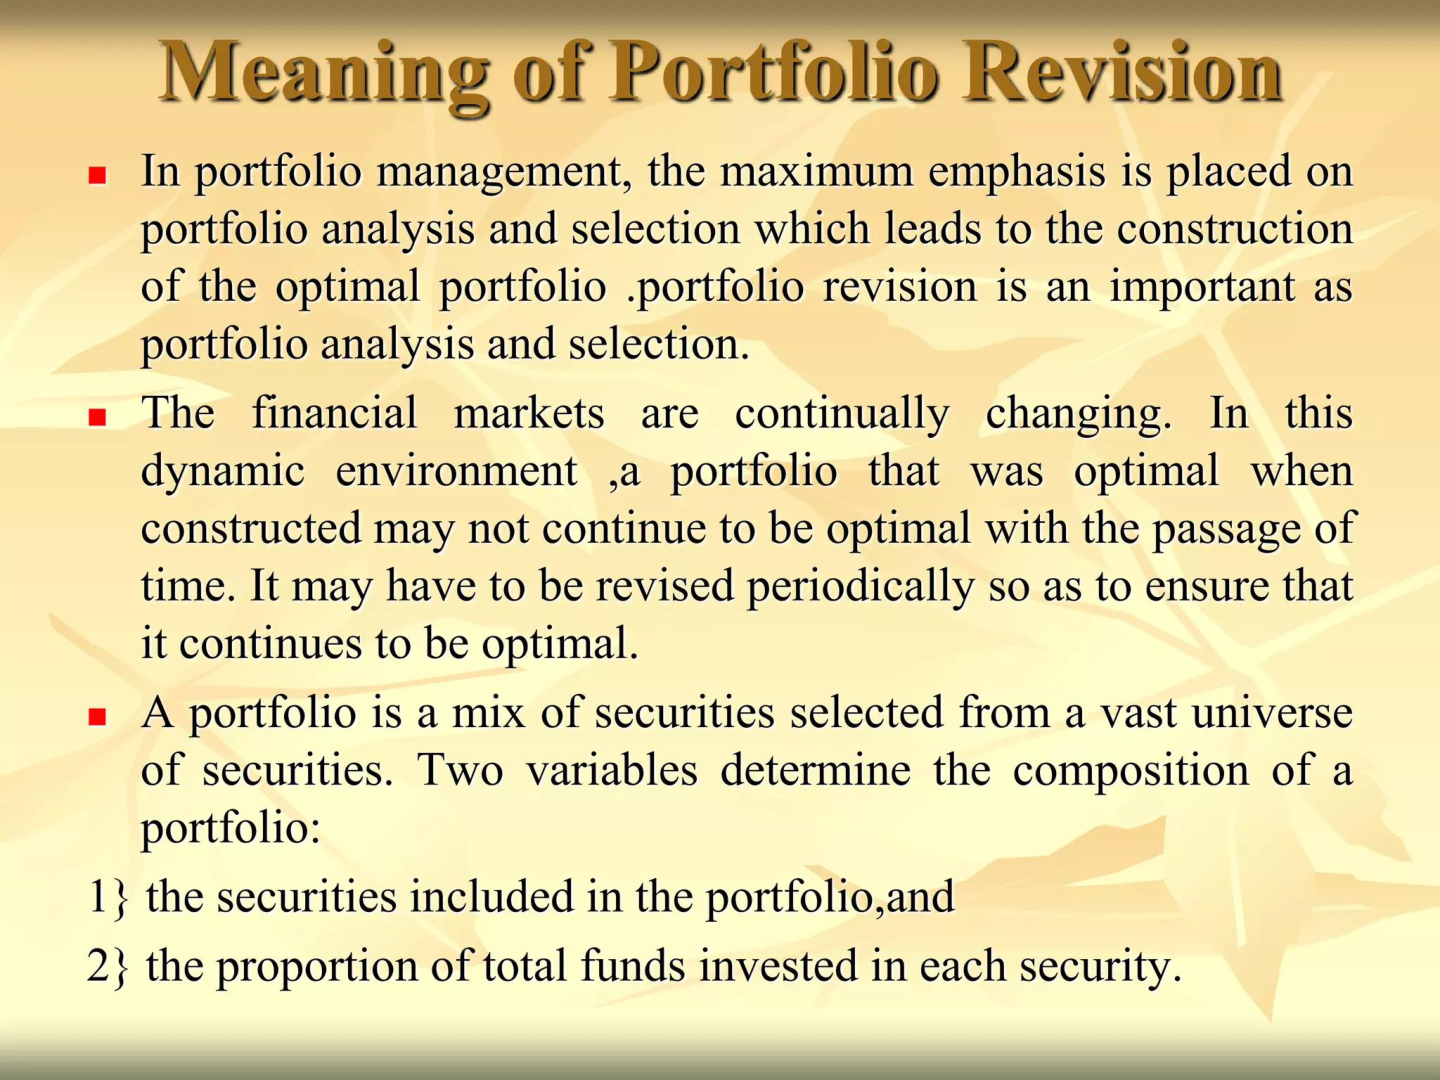
\includegraphics{figures/fig_0079.png}
\textgreater{} OCR cue: Meaning of Portfolio Revision = In portfolio
management, the maximum emphasis is placed on portfolio analysis and
selection which leads to the construction of the optimal portfolio
.portfolio revision is an important as portfolio analysis and selection.
=» The financial markets are continually changing. In this dynamic
environment ,a portfolio that was optimal when constructed may not
continue to

\hypertarget{figure-3-page-3}{%
\subsubsection{Figure 3 (Page 3)}\label{figure-3-page-3}}

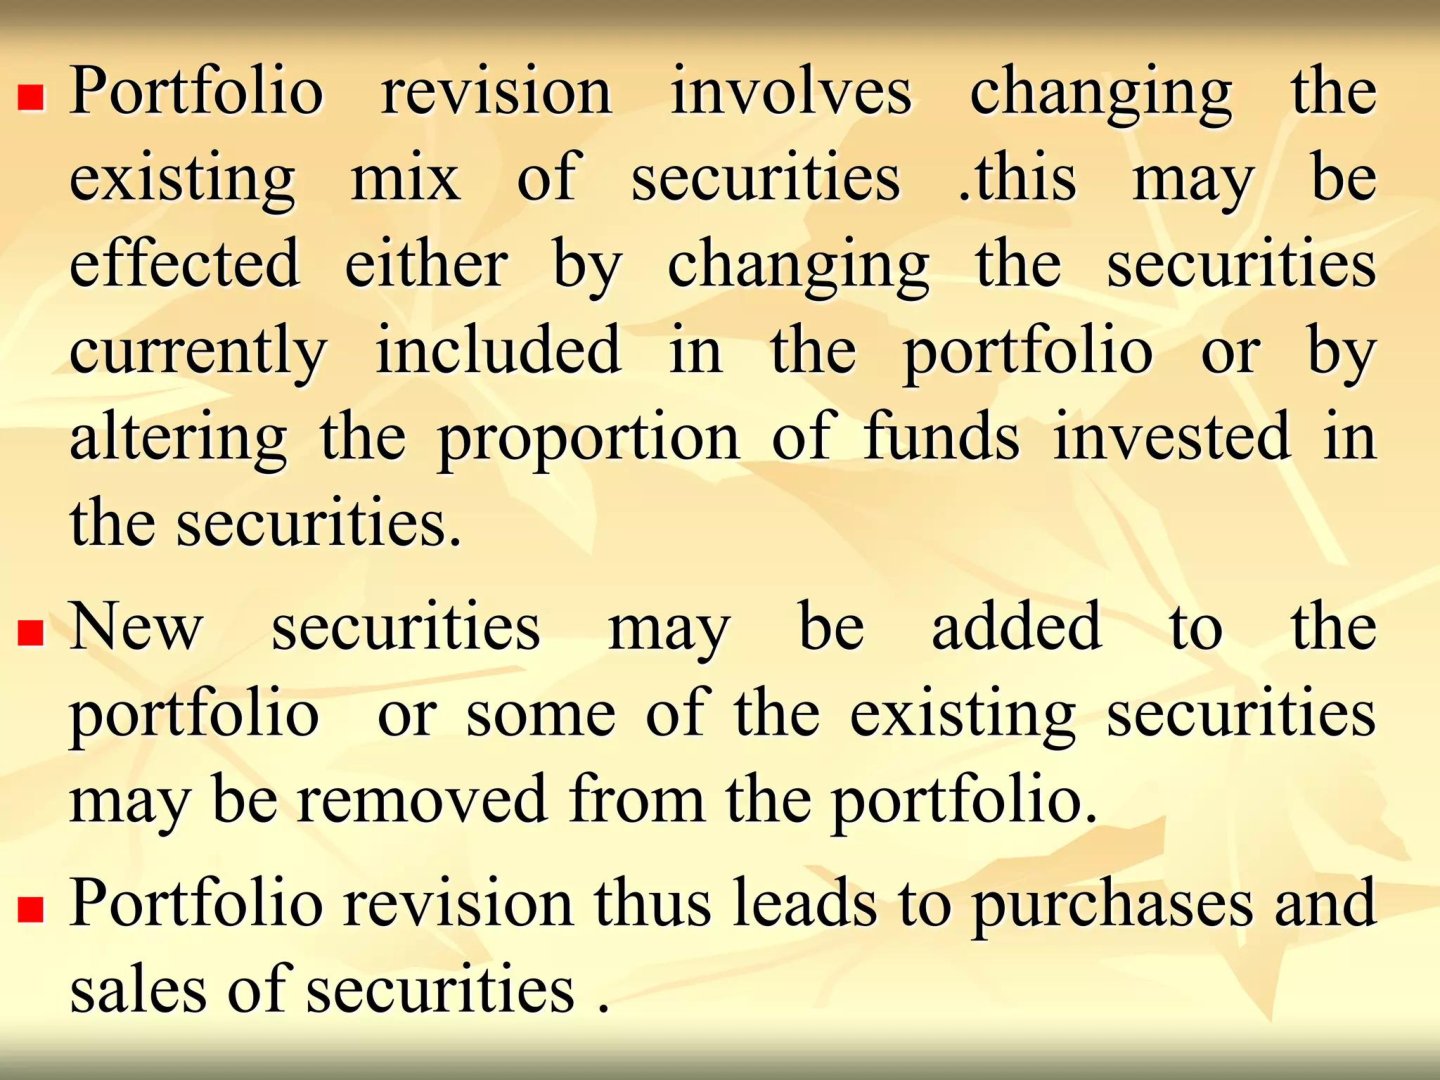
\includegraphics{figures/fig_0080.png}
\textgreater{} OCR cue: LE = Portfolio revision involves changing the
existing mix of securities .this may be effected either by changing the
securities currently included in the portfolio or by altering the
proportion of funds invested in the securities. =» New securities may be
added to the portfolio or some of the existing securities may be removed
from the portfolio. = Portfolio revision thus leads to purchases and s

\hypertarget{figure-4-page-4}{%
\subsubsection{Figure 4 (Page 4)}\label{figure-4-page-4}}

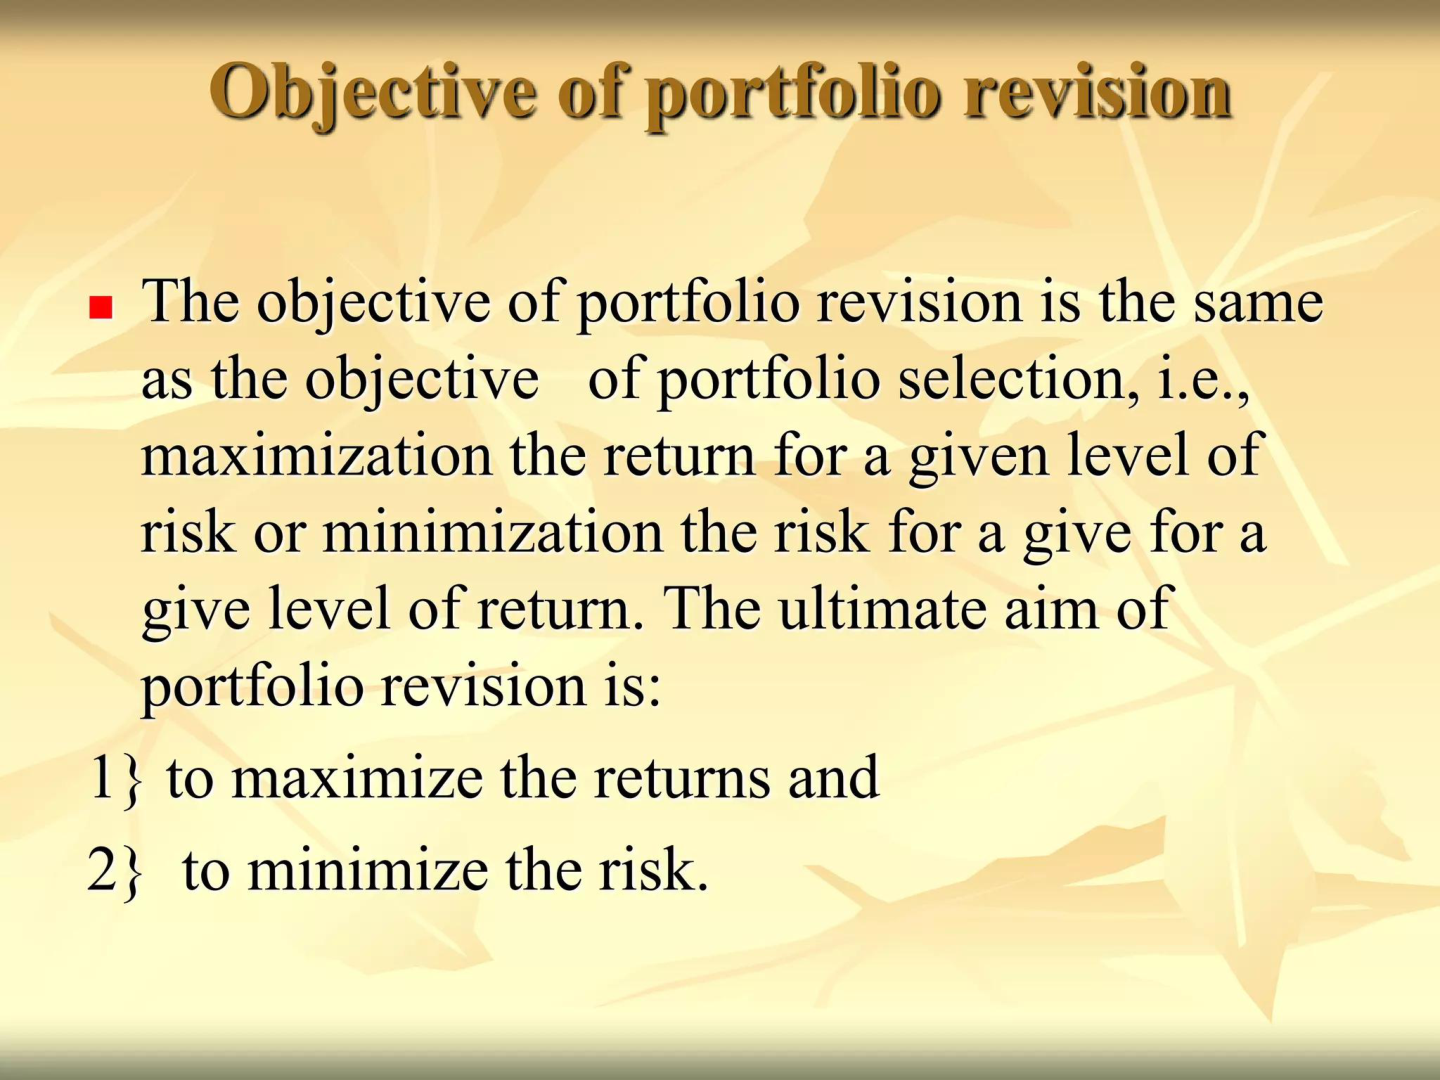
\includegraphics{figures/fig_0081.png}
\textgreater{} OCR cue: OO Objective of portfolio revision = The
objective of portfolio revision is the same as the objective of
portfolio selection, 1.e., maximization the return for a given level of
risk or minimization the risk for a give for a give level of return. The
ultimate aim of portfolio revision is: 1\} to maximize the returns and
2\} to minimize the risk.

\hypertarget{figure-5-page-5}{%
\subsubsection{Figure 5 (Page 5)}\label{figure-5-page-5}}

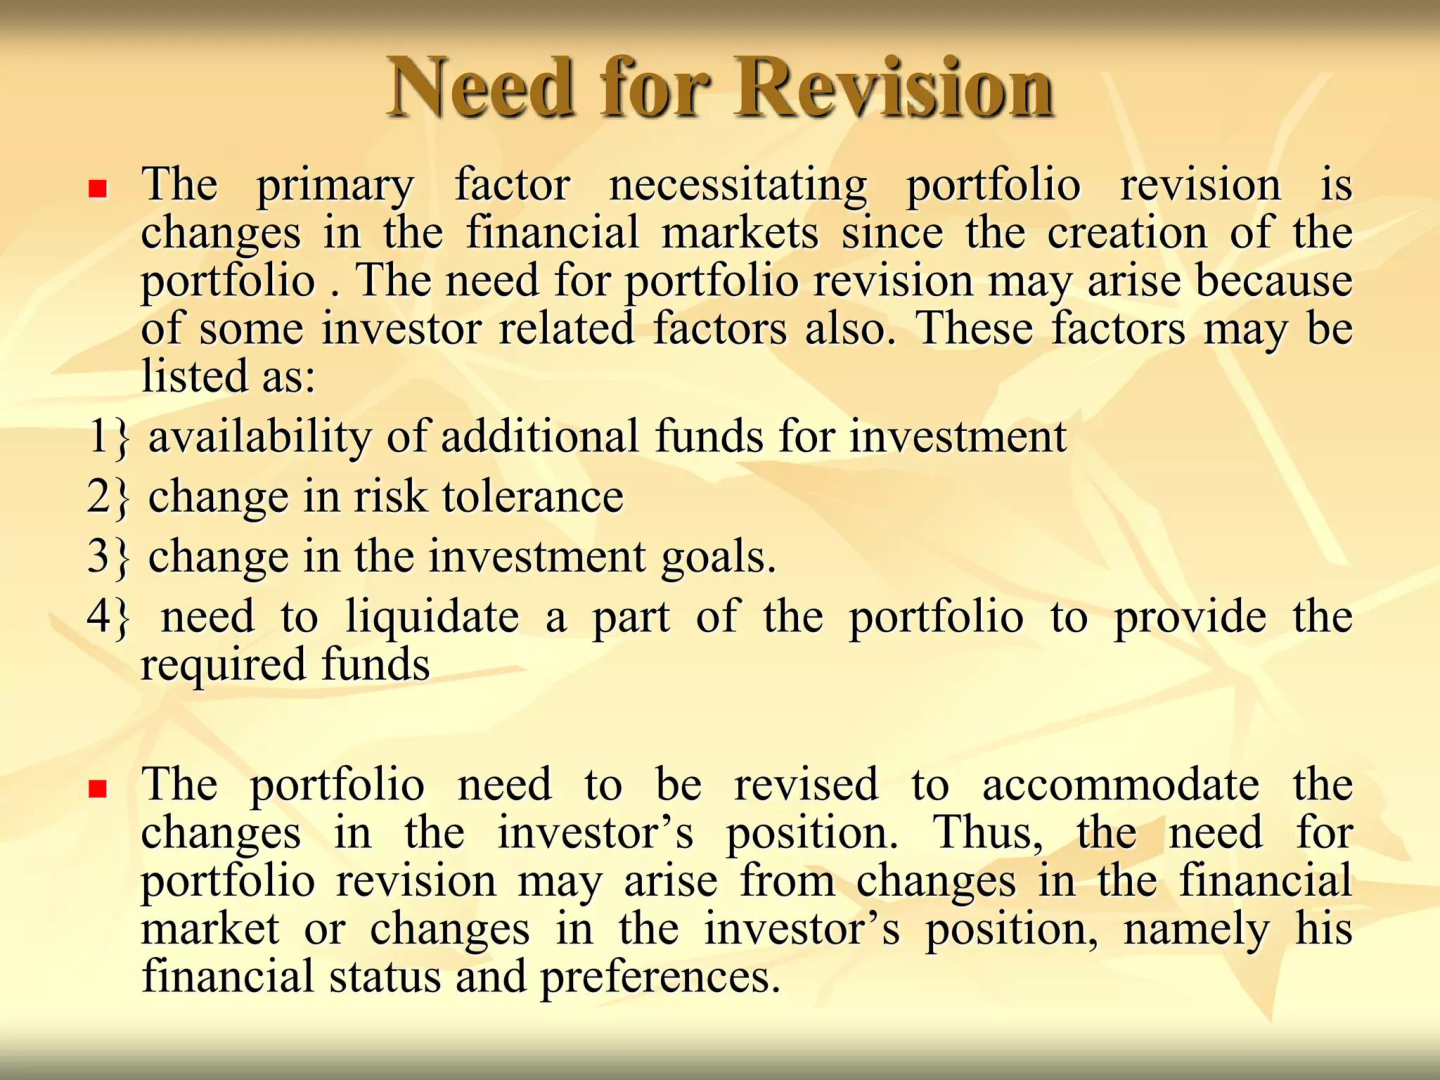
\includegraphics{figures/fig_0082.png}
\textgreater{} OCR cue: ee Need for Revision = The primary factor
necessitating portfolio revision is changes in the financial markets
since the creation of the portfolio . The need for portfolio revision
may arise because of some investor related factors also. These factors
may be listed as: 1\} availability of additional funds for investment
2~change in risk tolerance 3\} change in the investment goals. 4\} need
to liqui

\hypertarget{figure-6-page-6}{%
\subsubsection{Figure 6 (Page 6)}\label{figure-6-page-6}}

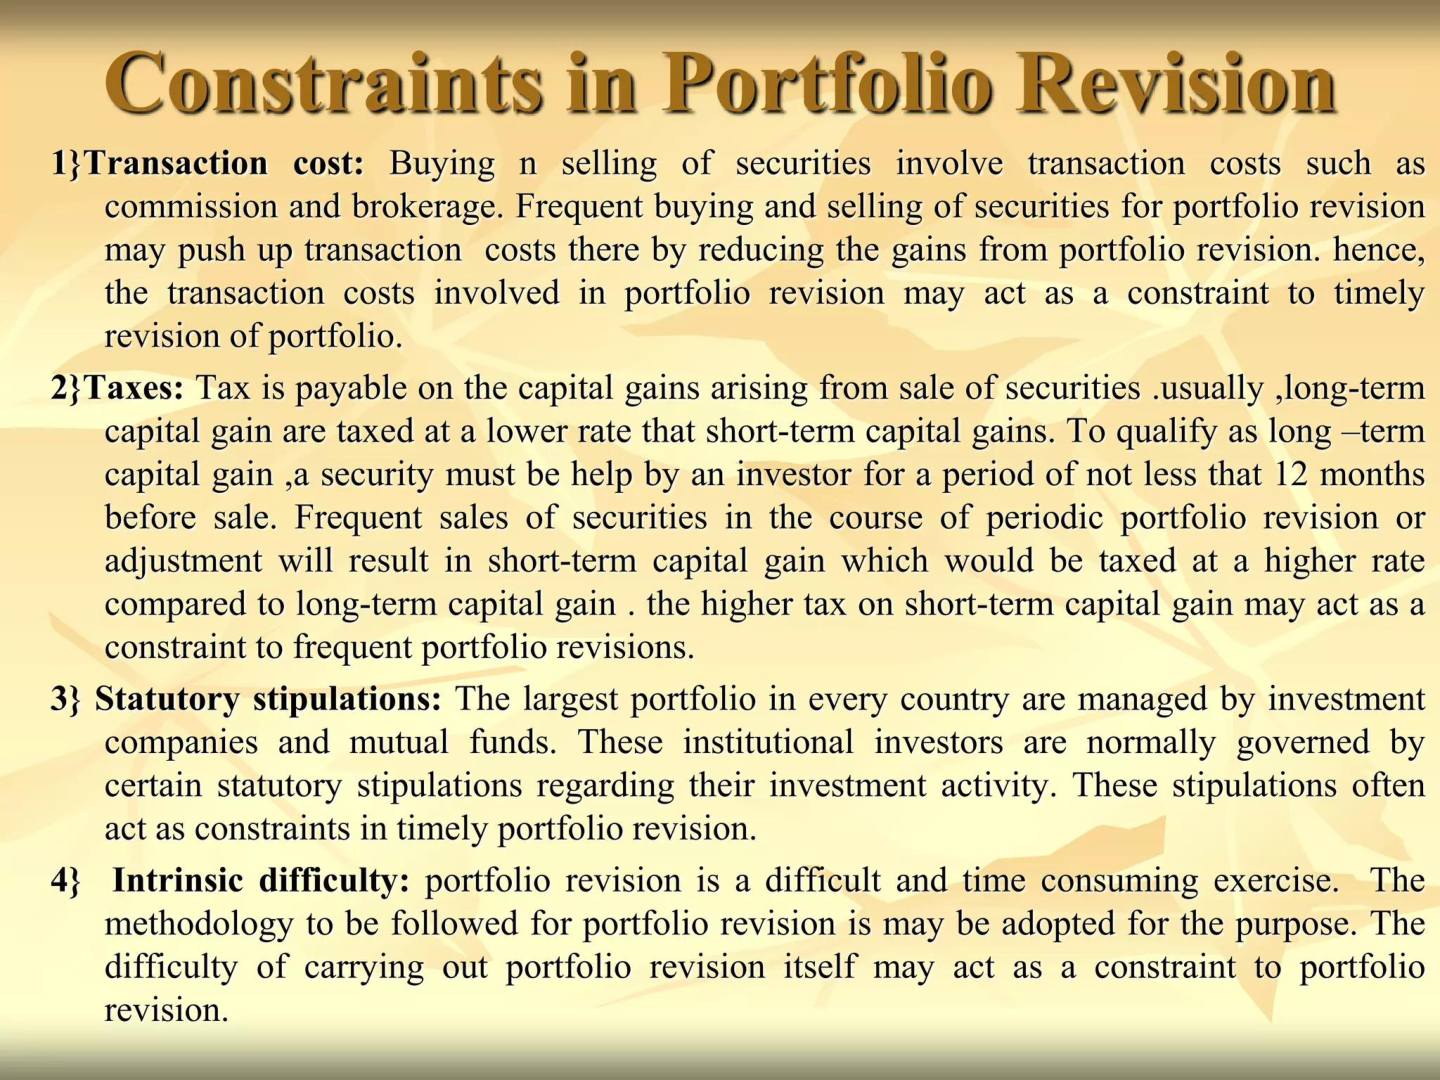
\includegraphics{figures/fig_0083.png}
\textgreater{} OCR cue: Constraints in Portfolio Revision 1\}Transaction
cost: Buying n selling of securities involve transaction costs such as
commission and brokerage. Frequent buying and selling of securities for
portfolio revision may push up transaction costs there by reducing the
gains from portfolio revision. hence, the transaction costs involved in
portfolio revision may act as a constraint to timely revision of p

\hypertarget{figure-7-page-7}{%
\subsubsection{Figure 7 (Page 7)}\label{figure-7-page-7}}

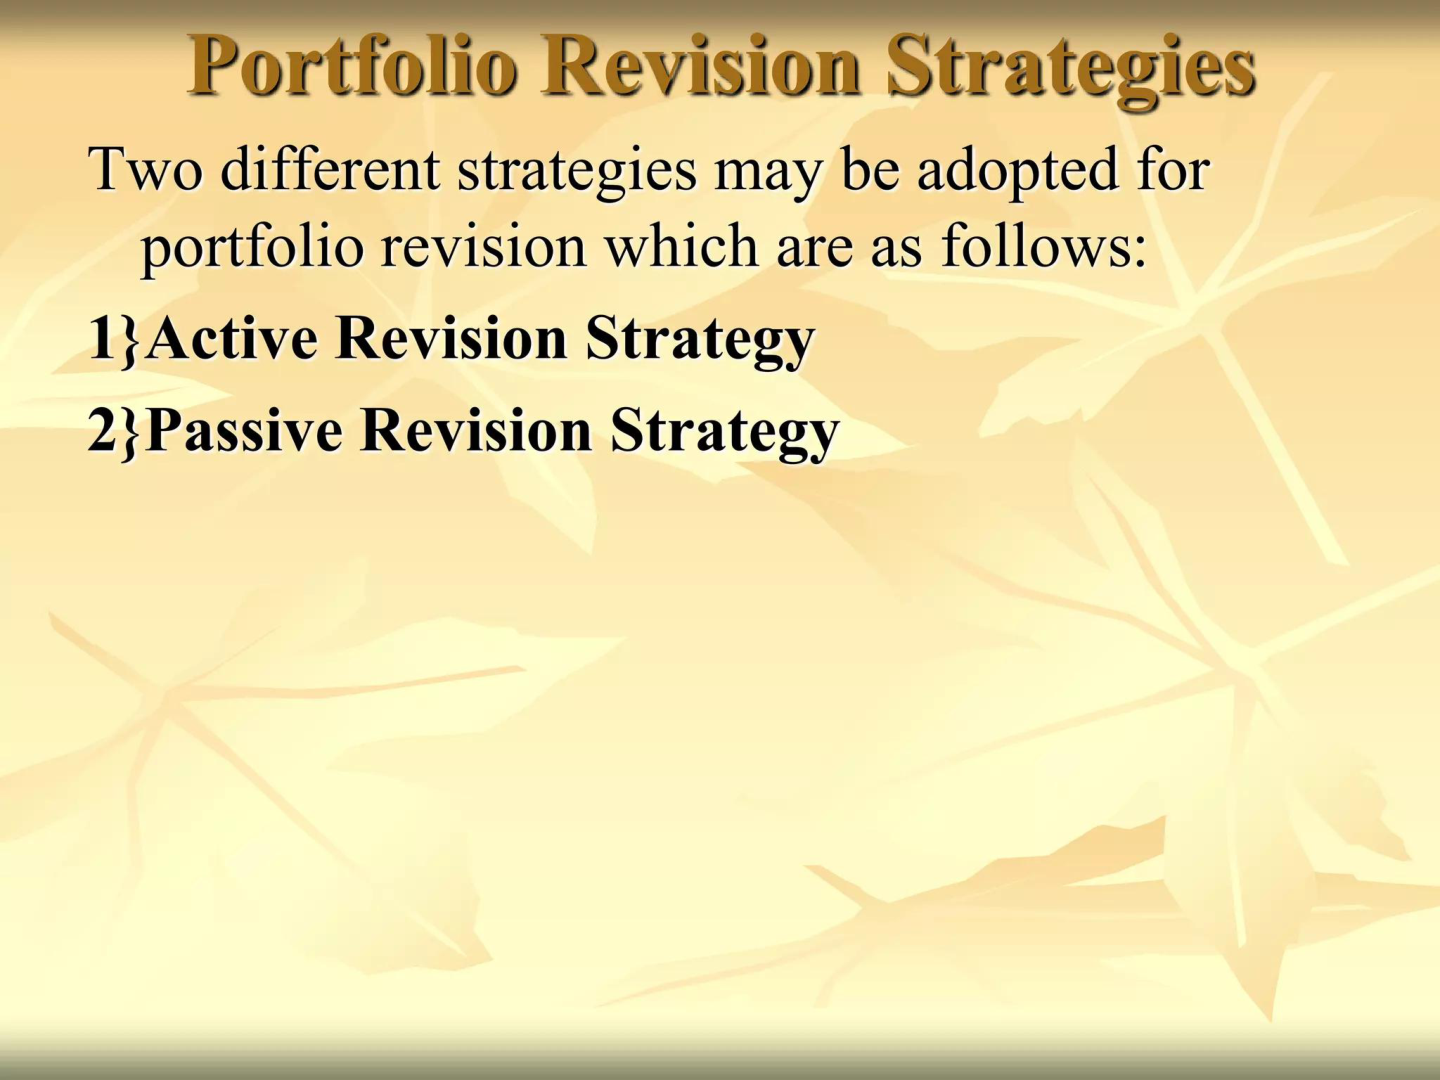
\includegraphics{figures/fig_0084.png}
\textgreater{} OCR cue: Two different strategies may be adopted for
portfolio revision which are as follows: 1\}Active Revision Strategy
2\}Passive Revision Strategy

\hypertarget{figure-8-page-8}{%
\subsubsection{Figure 8 (Page 8)}\label{figure-8-page-8}}

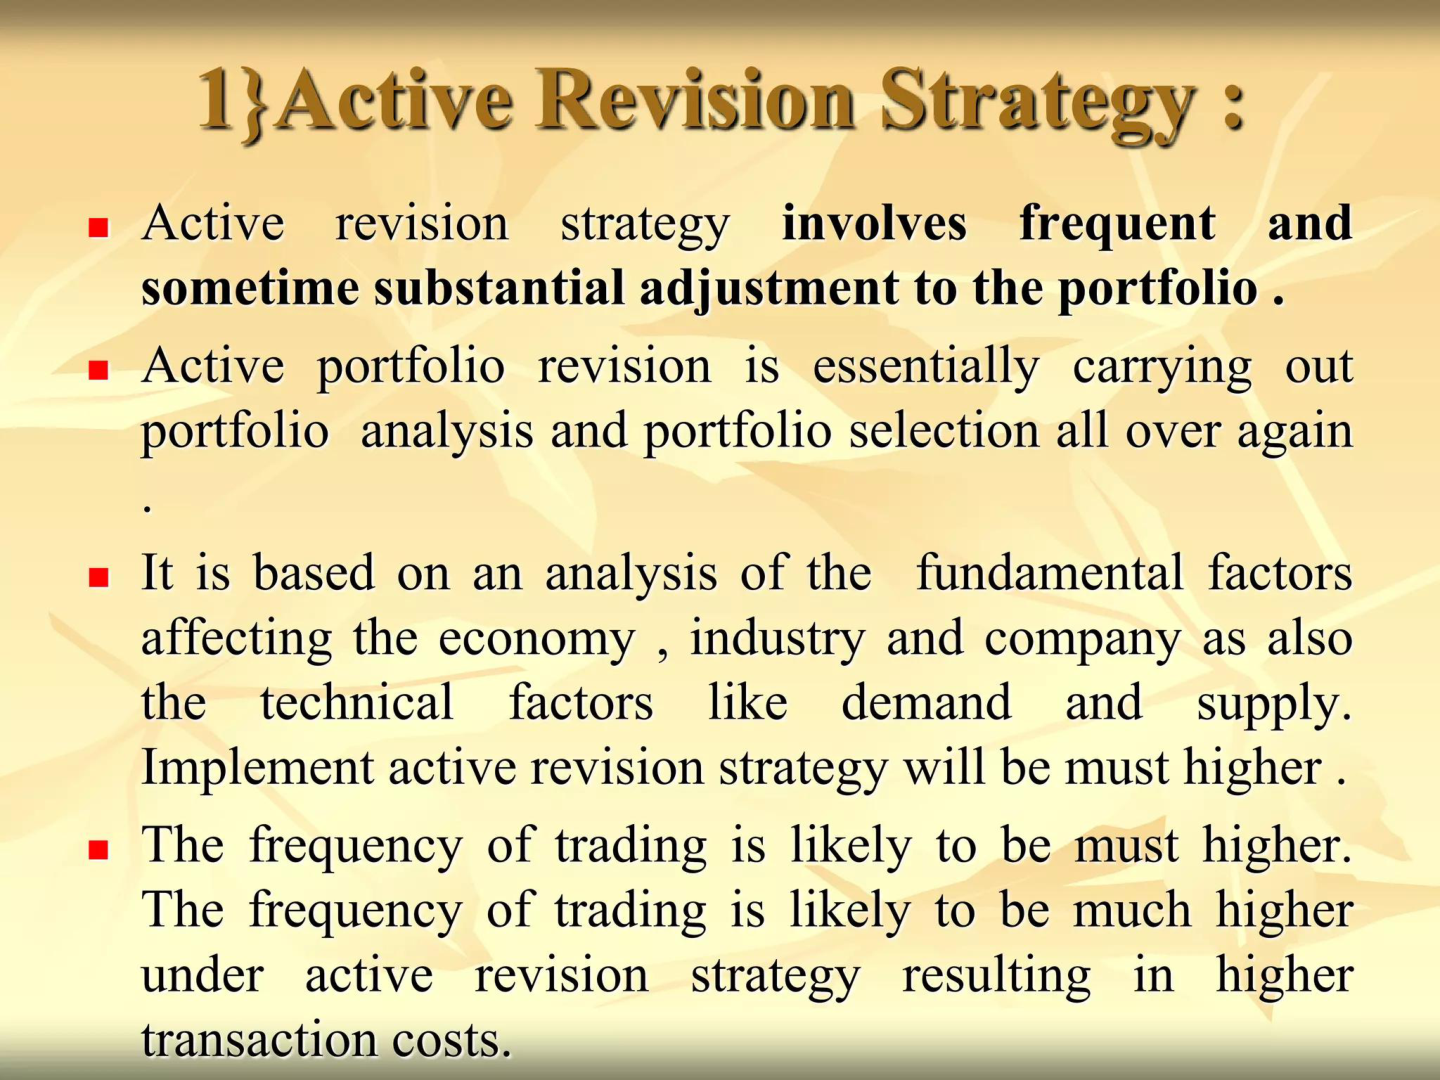
\includegraphics{figures/fig_0085.png}
\textgreater{} OCR cue: 1\}Active Revision Strategy : =» Active revision
strategy involves frequent and sometime substantial adjustment to the
portfolio . = Active portfolio revision is essentially carrying out
portfolio analysis and portfolio selection all over again = It is based
on an analysis of the fundamental factors affecting the economy ,
industry and company as also the technical factors like demand and \_
supply.

\hypertarget{figure-9-page-9}{%
\subsubsection{Figure 9 (Page 9)}\label{figure-9-page-9}}

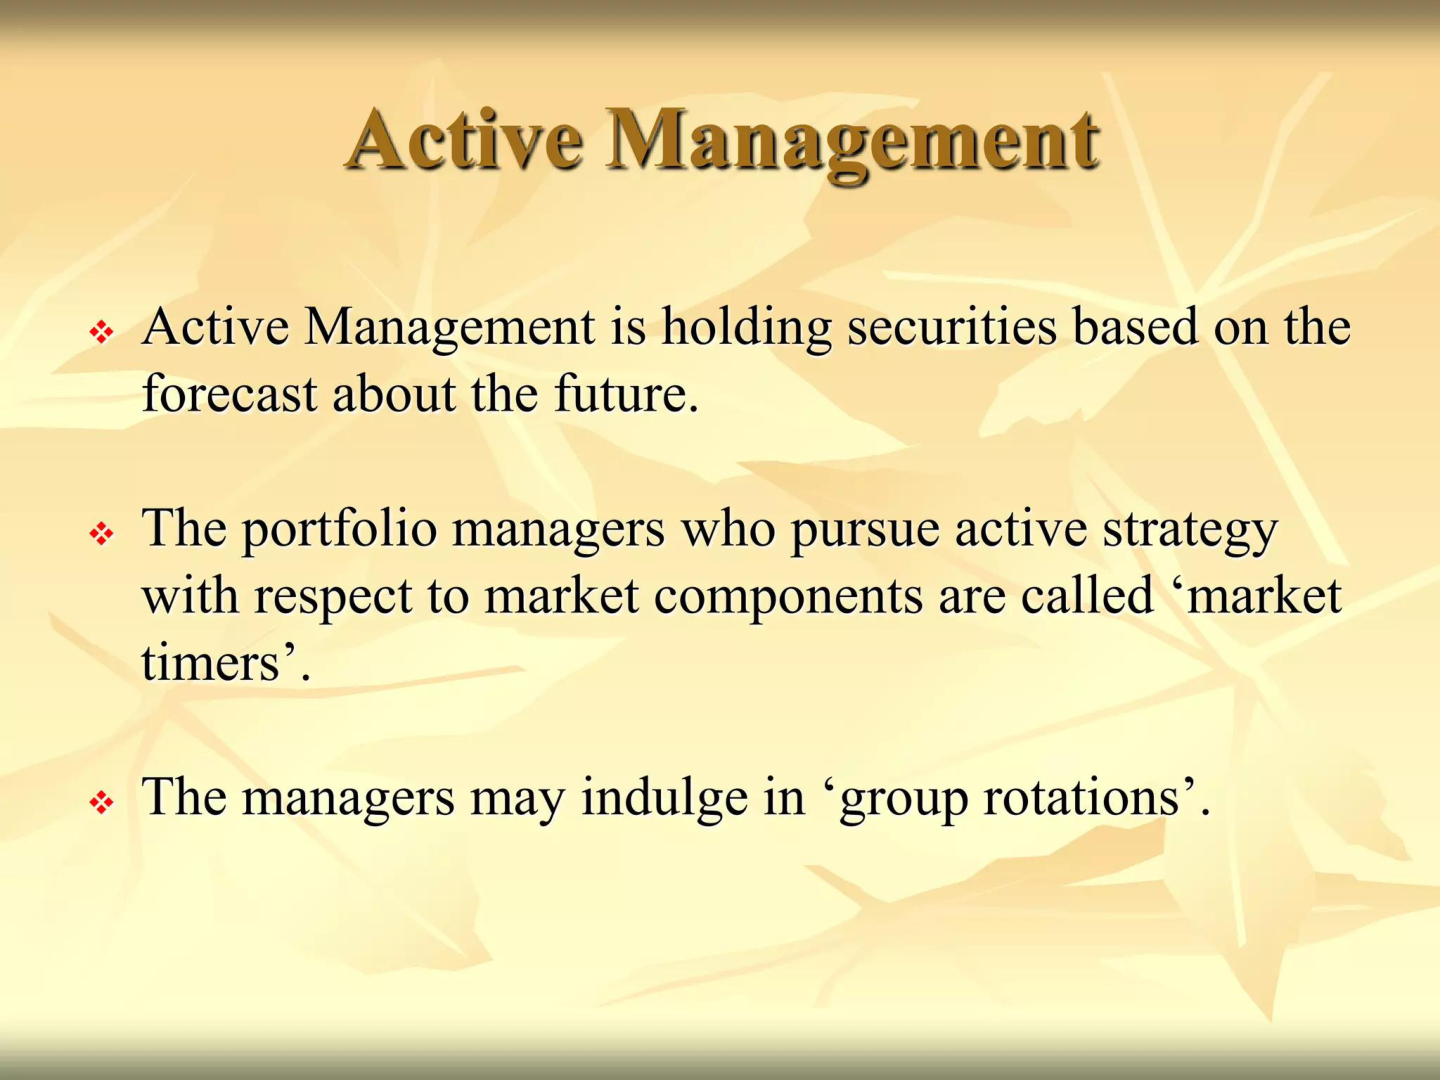
\includegraphics{figures/fig_0086.png}
\textgreater{} OCR cue: Active Management « Active Management is holding
securities based on the forecast about the future. « The portfolio
managers who pursue active strategy with respect to market components
are called `market timers'. « The managers may indulge in `group
rotations'.

\hypertarget{figure-10-page-10}{%
\subsubsection{Figure 10 (Page 10)}\label{figure-10-page-10}}

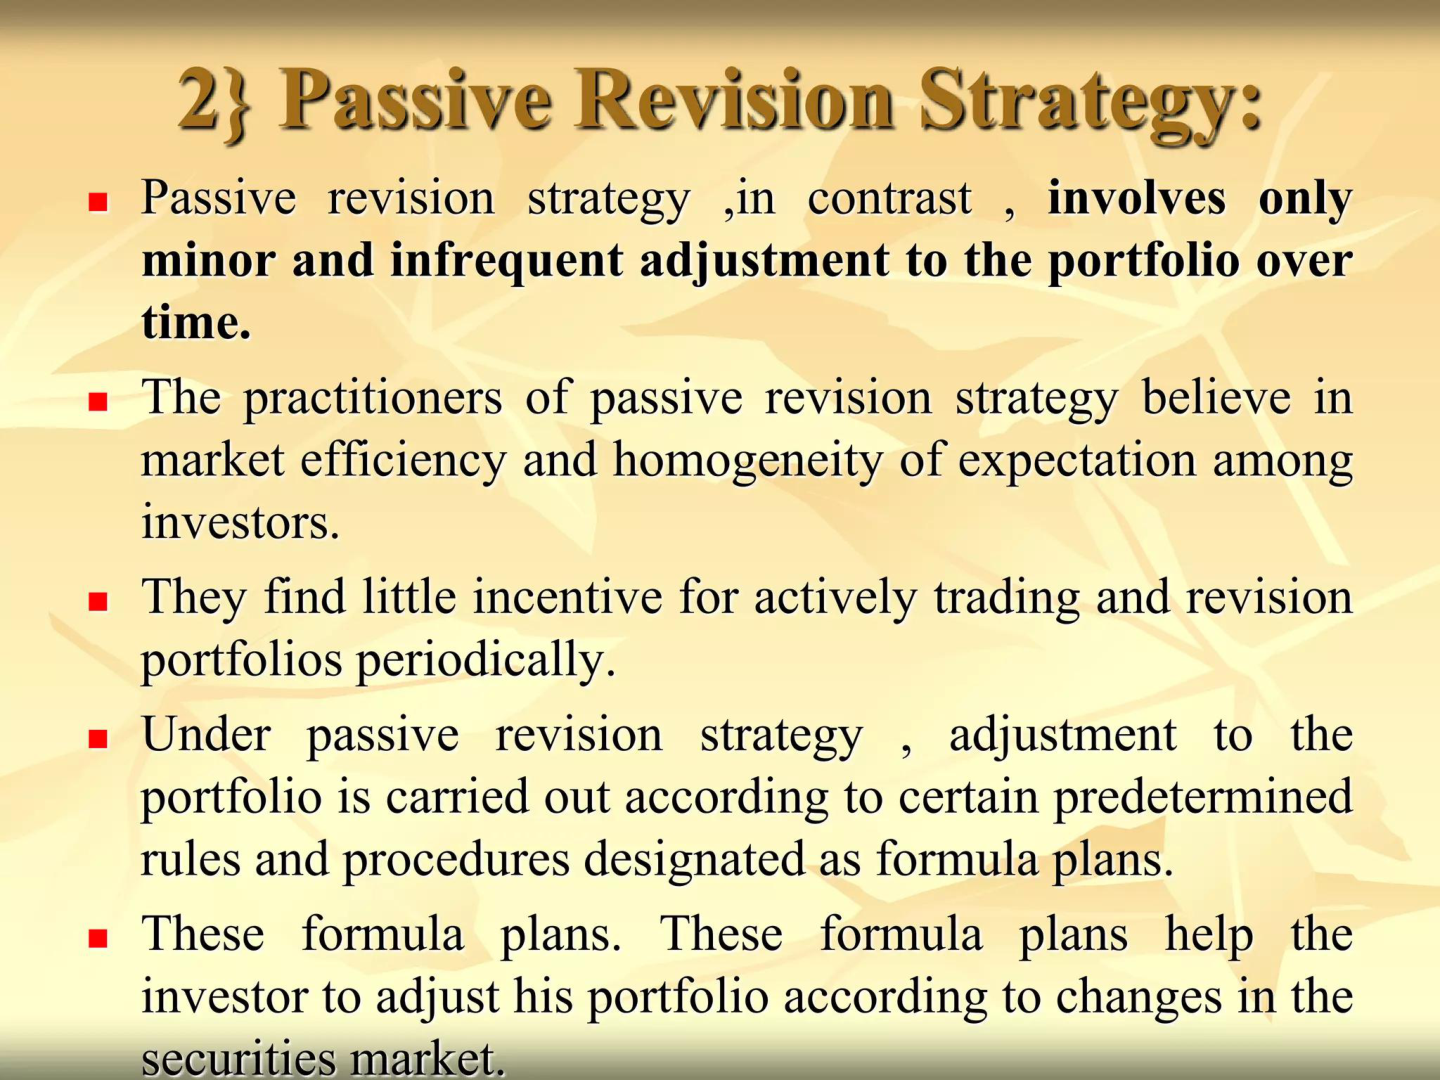
\includegraphics{figures/fig_0087.png}
\textgreater{} OCR cue: ee 2\} Passive Revision Strategy: = Passive
revision strategy ,in contrast , involves only minor and infrequent
adjustment to the portfolio over time. = The practitioners of passive
revision strategy believe in market efficiency and homogeneity of
expectation among investors. = They find little incentive for actively
trading and revision portfolios periodically. =» Under passive revision
strategy ,

\hypertarget{figure-11-page-11}{%
\subsubsection{Figure 11 (Page 11)}\label{figure-11-page-11}}

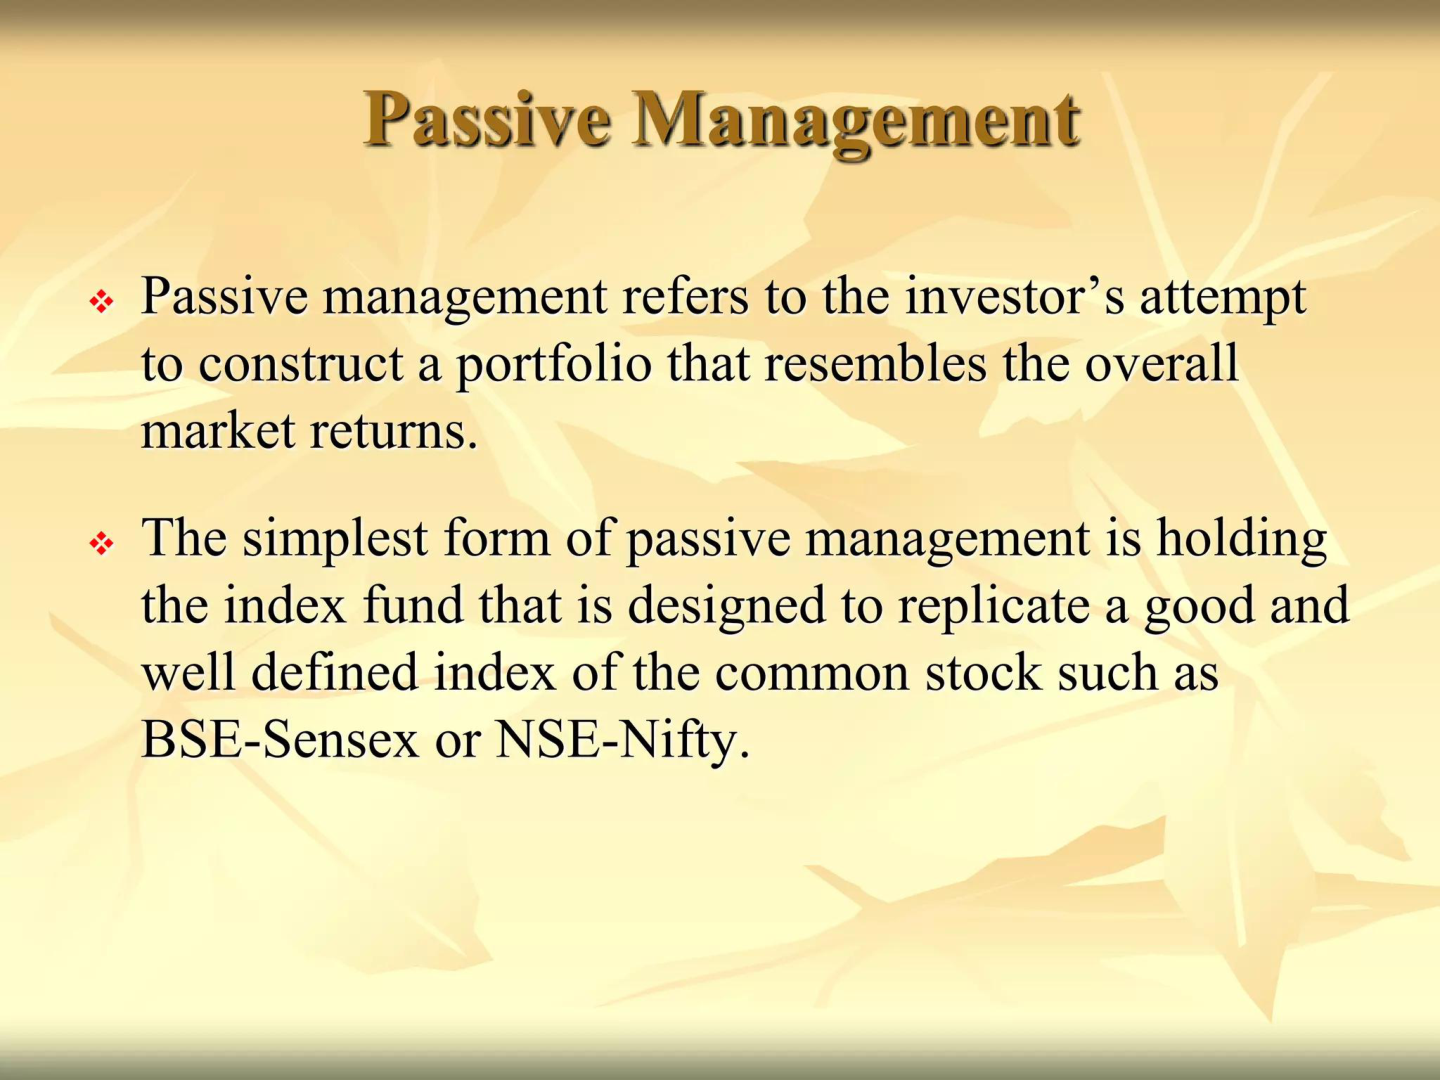
\includegraphics{figures/fig_0088.png}
\textgreater{} OCR cue: OO Passive Management « Passive management
refers to the investor's attempt to construct a portfolio that resembles
the overall market returns. « The simplest form of passive management is
holding the index fund that is designed to replicate a good and well
defined index of the common stock such as BSE-Sensex or NSE-Nifty.

\hypertarget{figure-12-page-12}{%
\subsubsection{Figure 12 (Page 12)}\label{figure-12-page-12}}

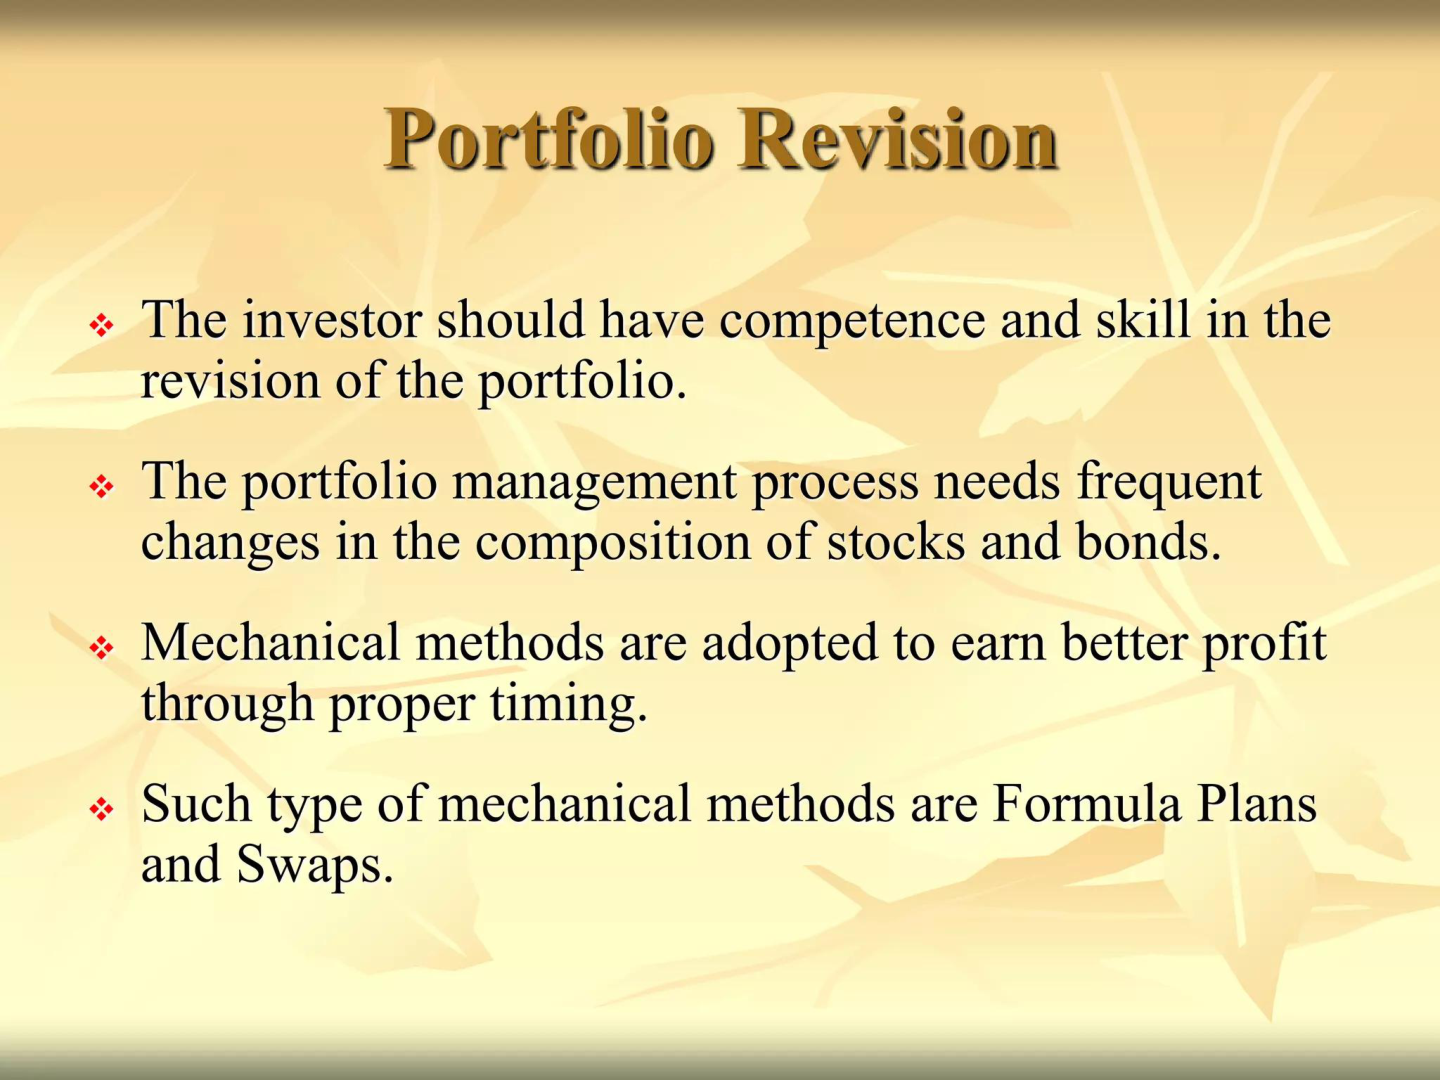
\includegraphics{figures/fig_0089.png}
\textgreater{} OCR cue: LSS SS\ldots{} Portfolio Revision « The investor
should have competence and skill in the revision of the portfolio. « The
portfolio management process needs frequent changes in the composition
of stocks and bonds. « Mechanical methods are adopted to earn better
profit through proper timing. « Such type of mechanical methods are
Formula Plans and Swaps.

\hypertarget{unit-62-sharpe-treynor-and-jensen.docx}{%
\subsection{UNIT 6/2 Sharpe, Treynor and
Jensen.docx}\label{unit-62-sharpe-treynor-and-jensen.docx}}

\hypertarget{figure-1-image-1}{%
\subsubsection{Figure 1 (Image)}\label{figure-1-image-1}}

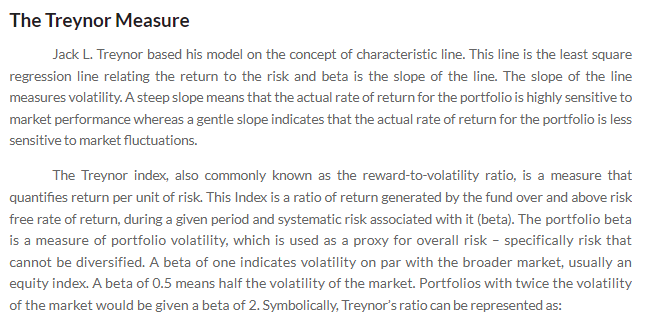
\includegraphics{figures/fig_0090.png}
\textgreater{} OCR cue: The Treynor Measure Jack L. Treynor based his
model on the concept of characteristic line. This line is the least
square regression line relating the return to the risk and beta is the
slope of the line. The slope of the line measures volatility. A steep
slope means that the actual rate of return for the portfolio is highly
sensitive to market performance whereas a gentle slope indicates that
the

\hypertarget{figure-2-image}{%
\subsubsection{Figure 2 (Image)}\label{figure-2-image}}

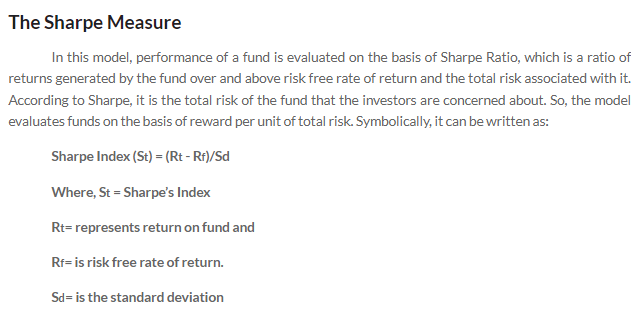
\includegraphics{figures/fig_0091.png}
\textgreater{} OCR cue: The Sharpe Measure In this model, performance of
a fund is evaluated on the basis of Sharpe Ratio, which is a ratio of
returns generated by the fund over and above risk free rate of return
and the total risk associated with it According to Sharpe, itis the
total risk of the fund that the investors are concerned about. So, the
model evaluates funds on the basis of reward per unit of total risk. Sym

\hypertarget{figure-3-image}{%
\subsubsection{Figure 3 (Image)}\label{figure-3-image}}

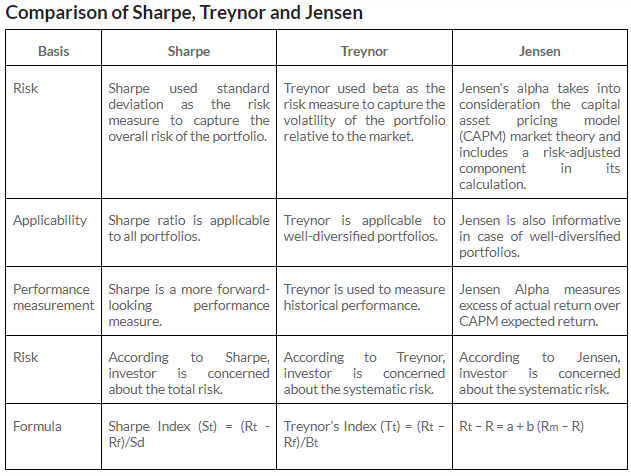
\includegraphics{figures/fig_0092.png}
\textgreater{} OCR cue: Comparison of Sharpe, Treynor and Jensen Basis
Sharpe Treynor Jensen Risk Sharpe used \_ standard deviation as the risk
measure to capture the overall risk of the portfolio. 'Treynor used beta
as the risk measure to capture the volatility of the portfolio relative
to the market. Jensen's alpha takes into consideration the capital asset
pricing model (CAPM) market theory and includes a risk-adjusted

\hypertarget{figure-4-image}{%
\subsubsection{Figure 4 (Image)}\label{figure-4-image}}

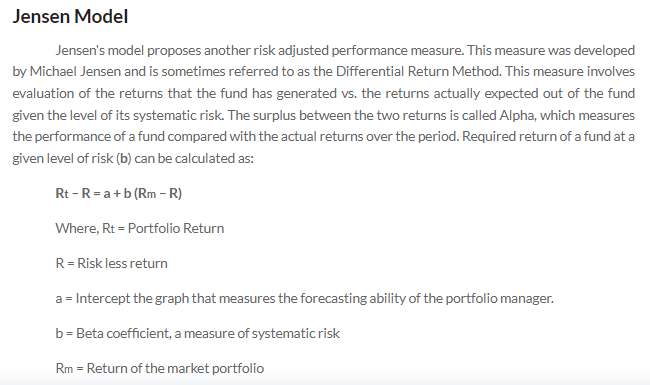
\includegraphics{figures/fig_0093.png}
\textgreater{} OCR cue: Jensen Model Jensen's model proposes another
risk adjusted performance measure. This measure was developed by Michael
Jensen and is sometimes referred to as the Differential Return Method.
This measure involves evaluation of the returns that the fund has
generated vs.~the returns actually expected out of the fund given the
level of its systematic risk. The surplus between the two returns is
called

\hypertarget{figure-5-image}{%
\subsubsection{Figure 5 (Image)}\label{figure-5-image}}

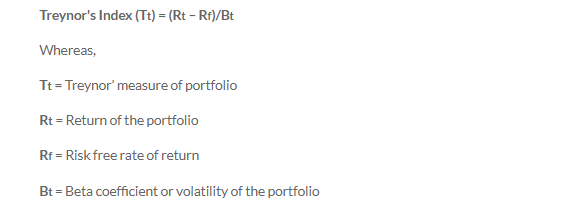
\includegraphics{figures/fig_0094.png}
\textgreater{} OCR cue: Treynor's Index (Tt) = (Rt - Re)/Bt Whereas,
`Tt=Treynor' measure of portfolio Rt= Return of the portfolio Rr= Risk
free rate of return Bt= Beta coefficient or volatility of the portfolio

\hypertarget{unit-62.2-numericals-sharpe-treynor-jensen.pdf}{%
\subsection{UNIT 6/2.2 Numericals Sharpe, Treynor,
Jensen.pdf}\label{unit-62.2-numericals-sharpe-treynor-jensen.pdf}}

\hypertarget{figure-1-page-1-1}{%
\subsubsection{Figure 1 (Page 1)}\label{figure-1-page-1-1}}

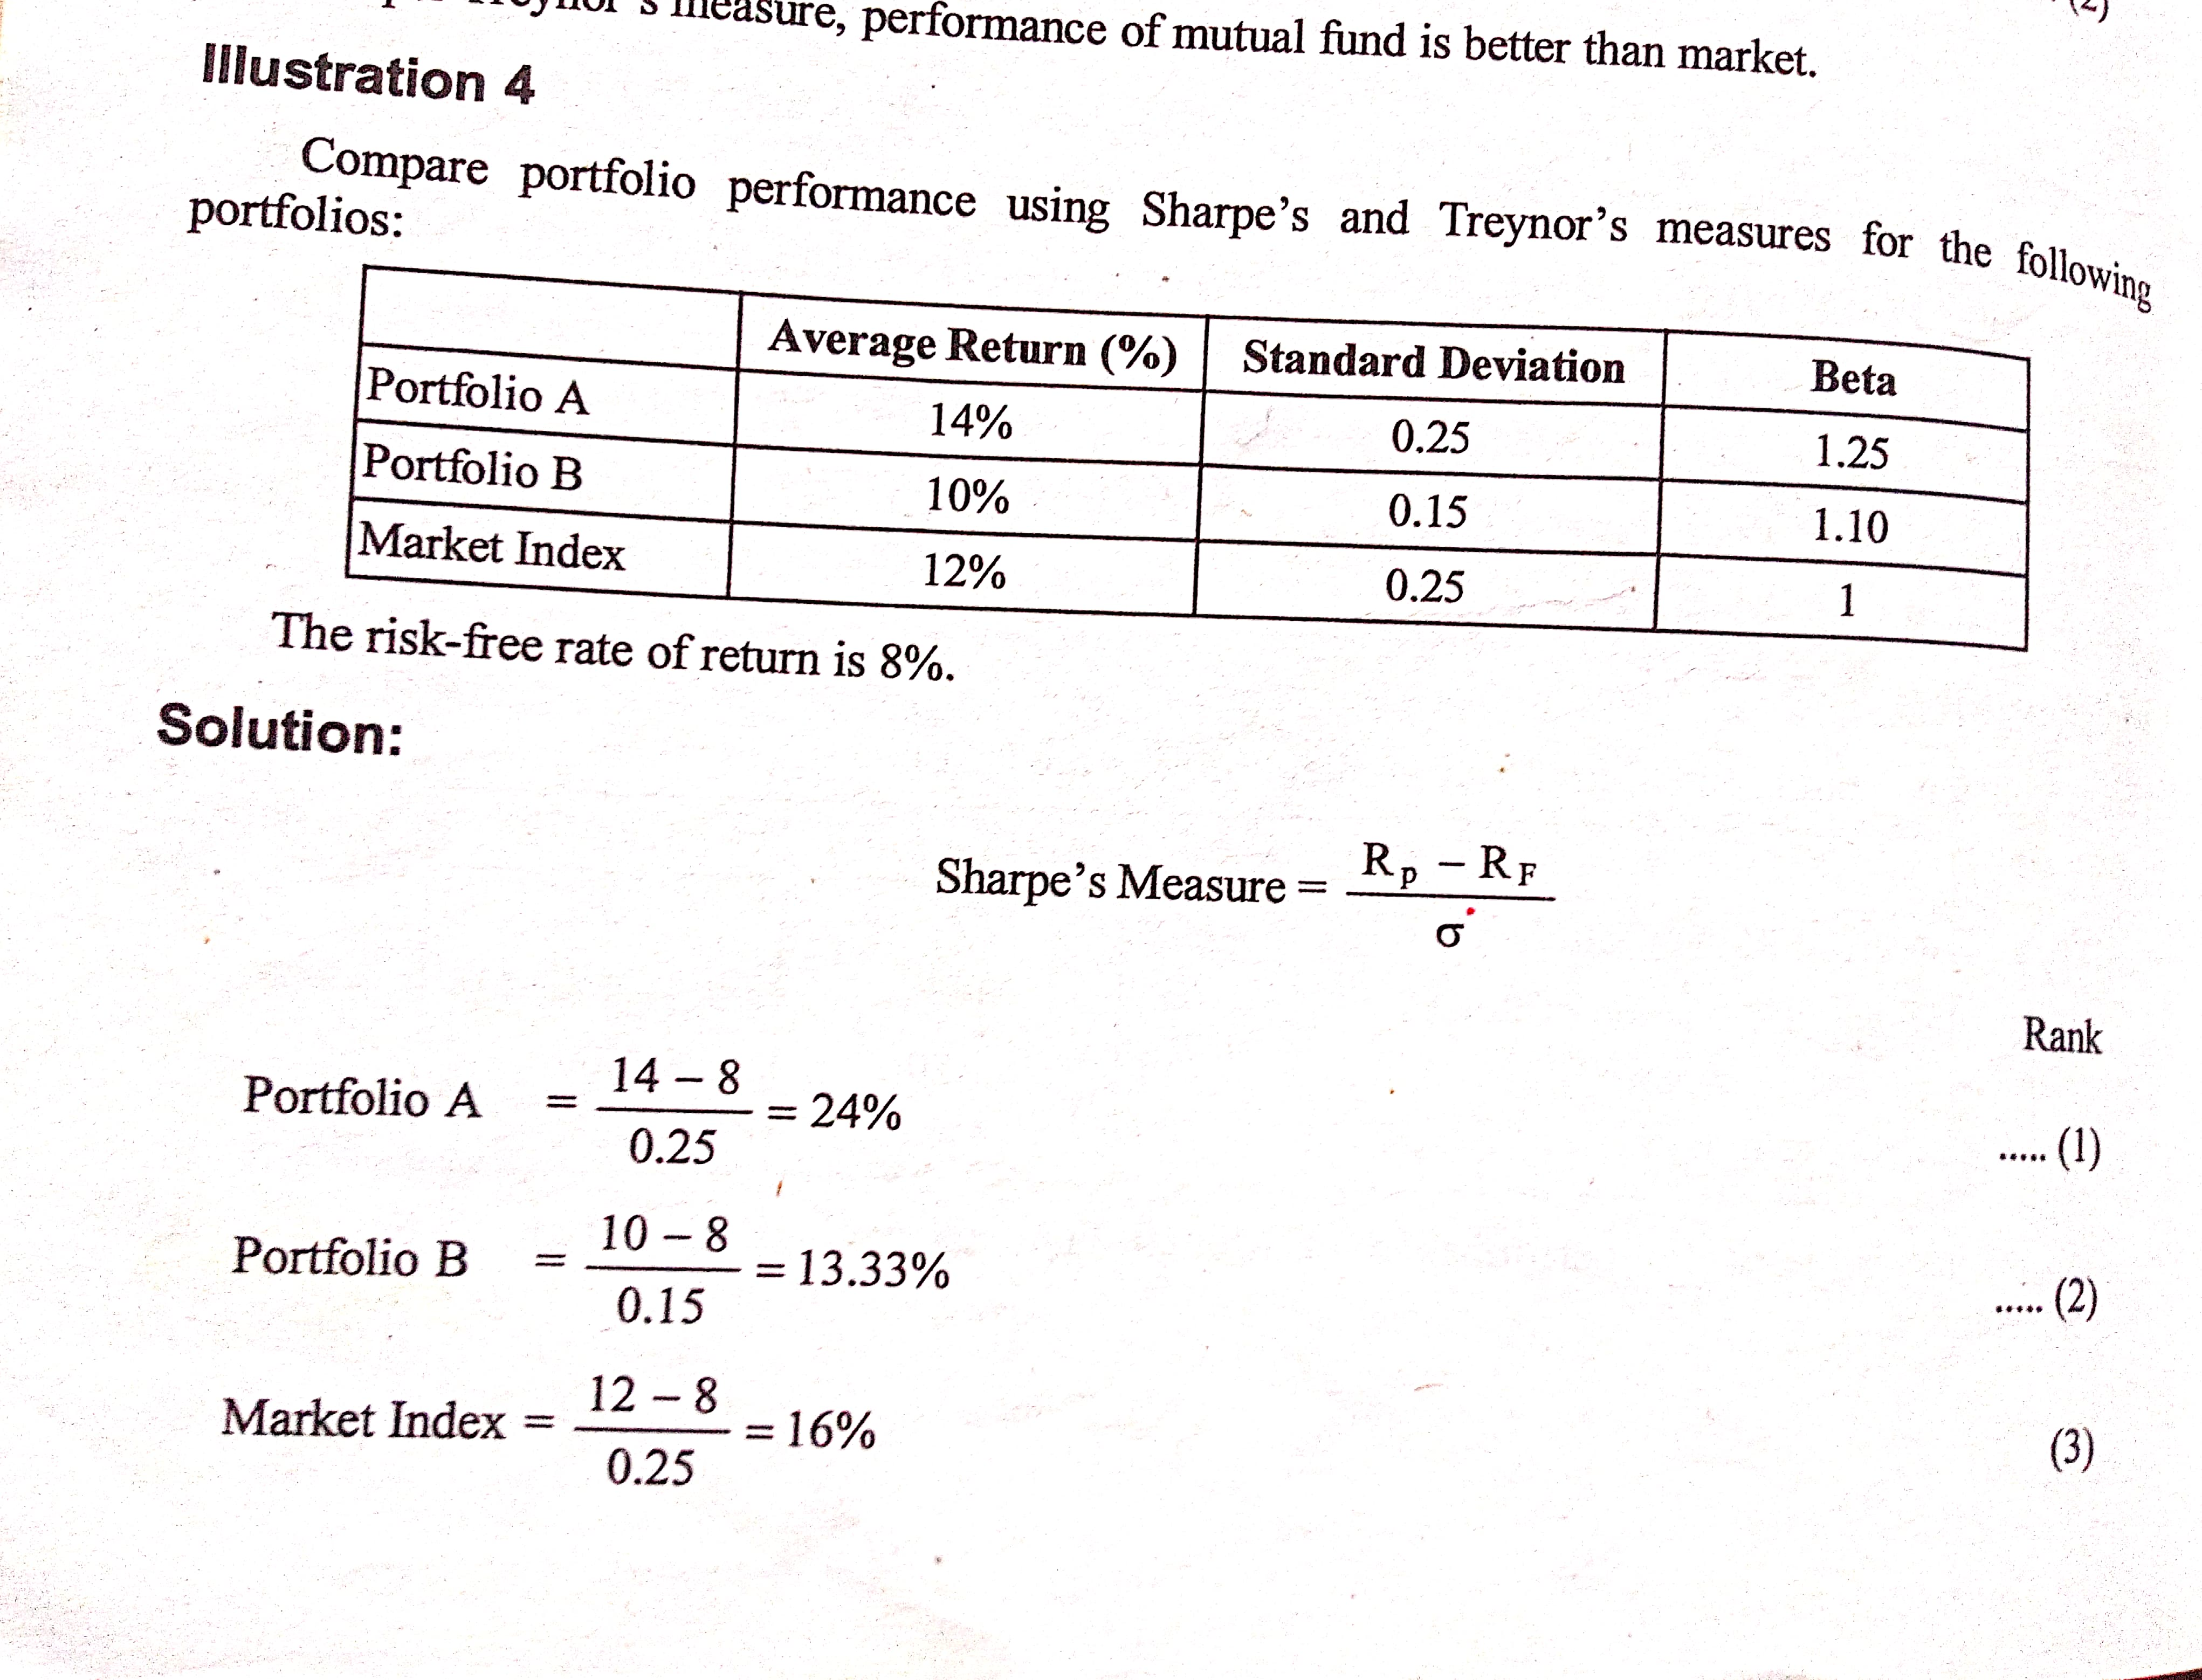
\includegraphics{figures/fig_0095.jpeg}
\textgreater{} OCR cue: eh ead nie EN ESNTE, Performance of mutual fund
is better than market. lllustration 4 \textbar{} ; Compare portfolios: 2
: * Average Return (\%) \textbar{} Standard Deviation The risk-free rate
of return is 8\%. portfolio Performance using Sharpe's and Treynor's
measures for the follow: Wing a \$ fo) \textgreater{} S E a a is
Solution: Sharpe's Measure = Rp oR oO Rank Portfolio A = = = 249\%, Ea
Sate \textbar{} ahaa (1) PortfolioB = 7 --- = 1

\hypertarget{figure-2-page-2-1}{%
\subsubsection{Figure 2 (Page 2)}\label{figure-2-page-2-1}}

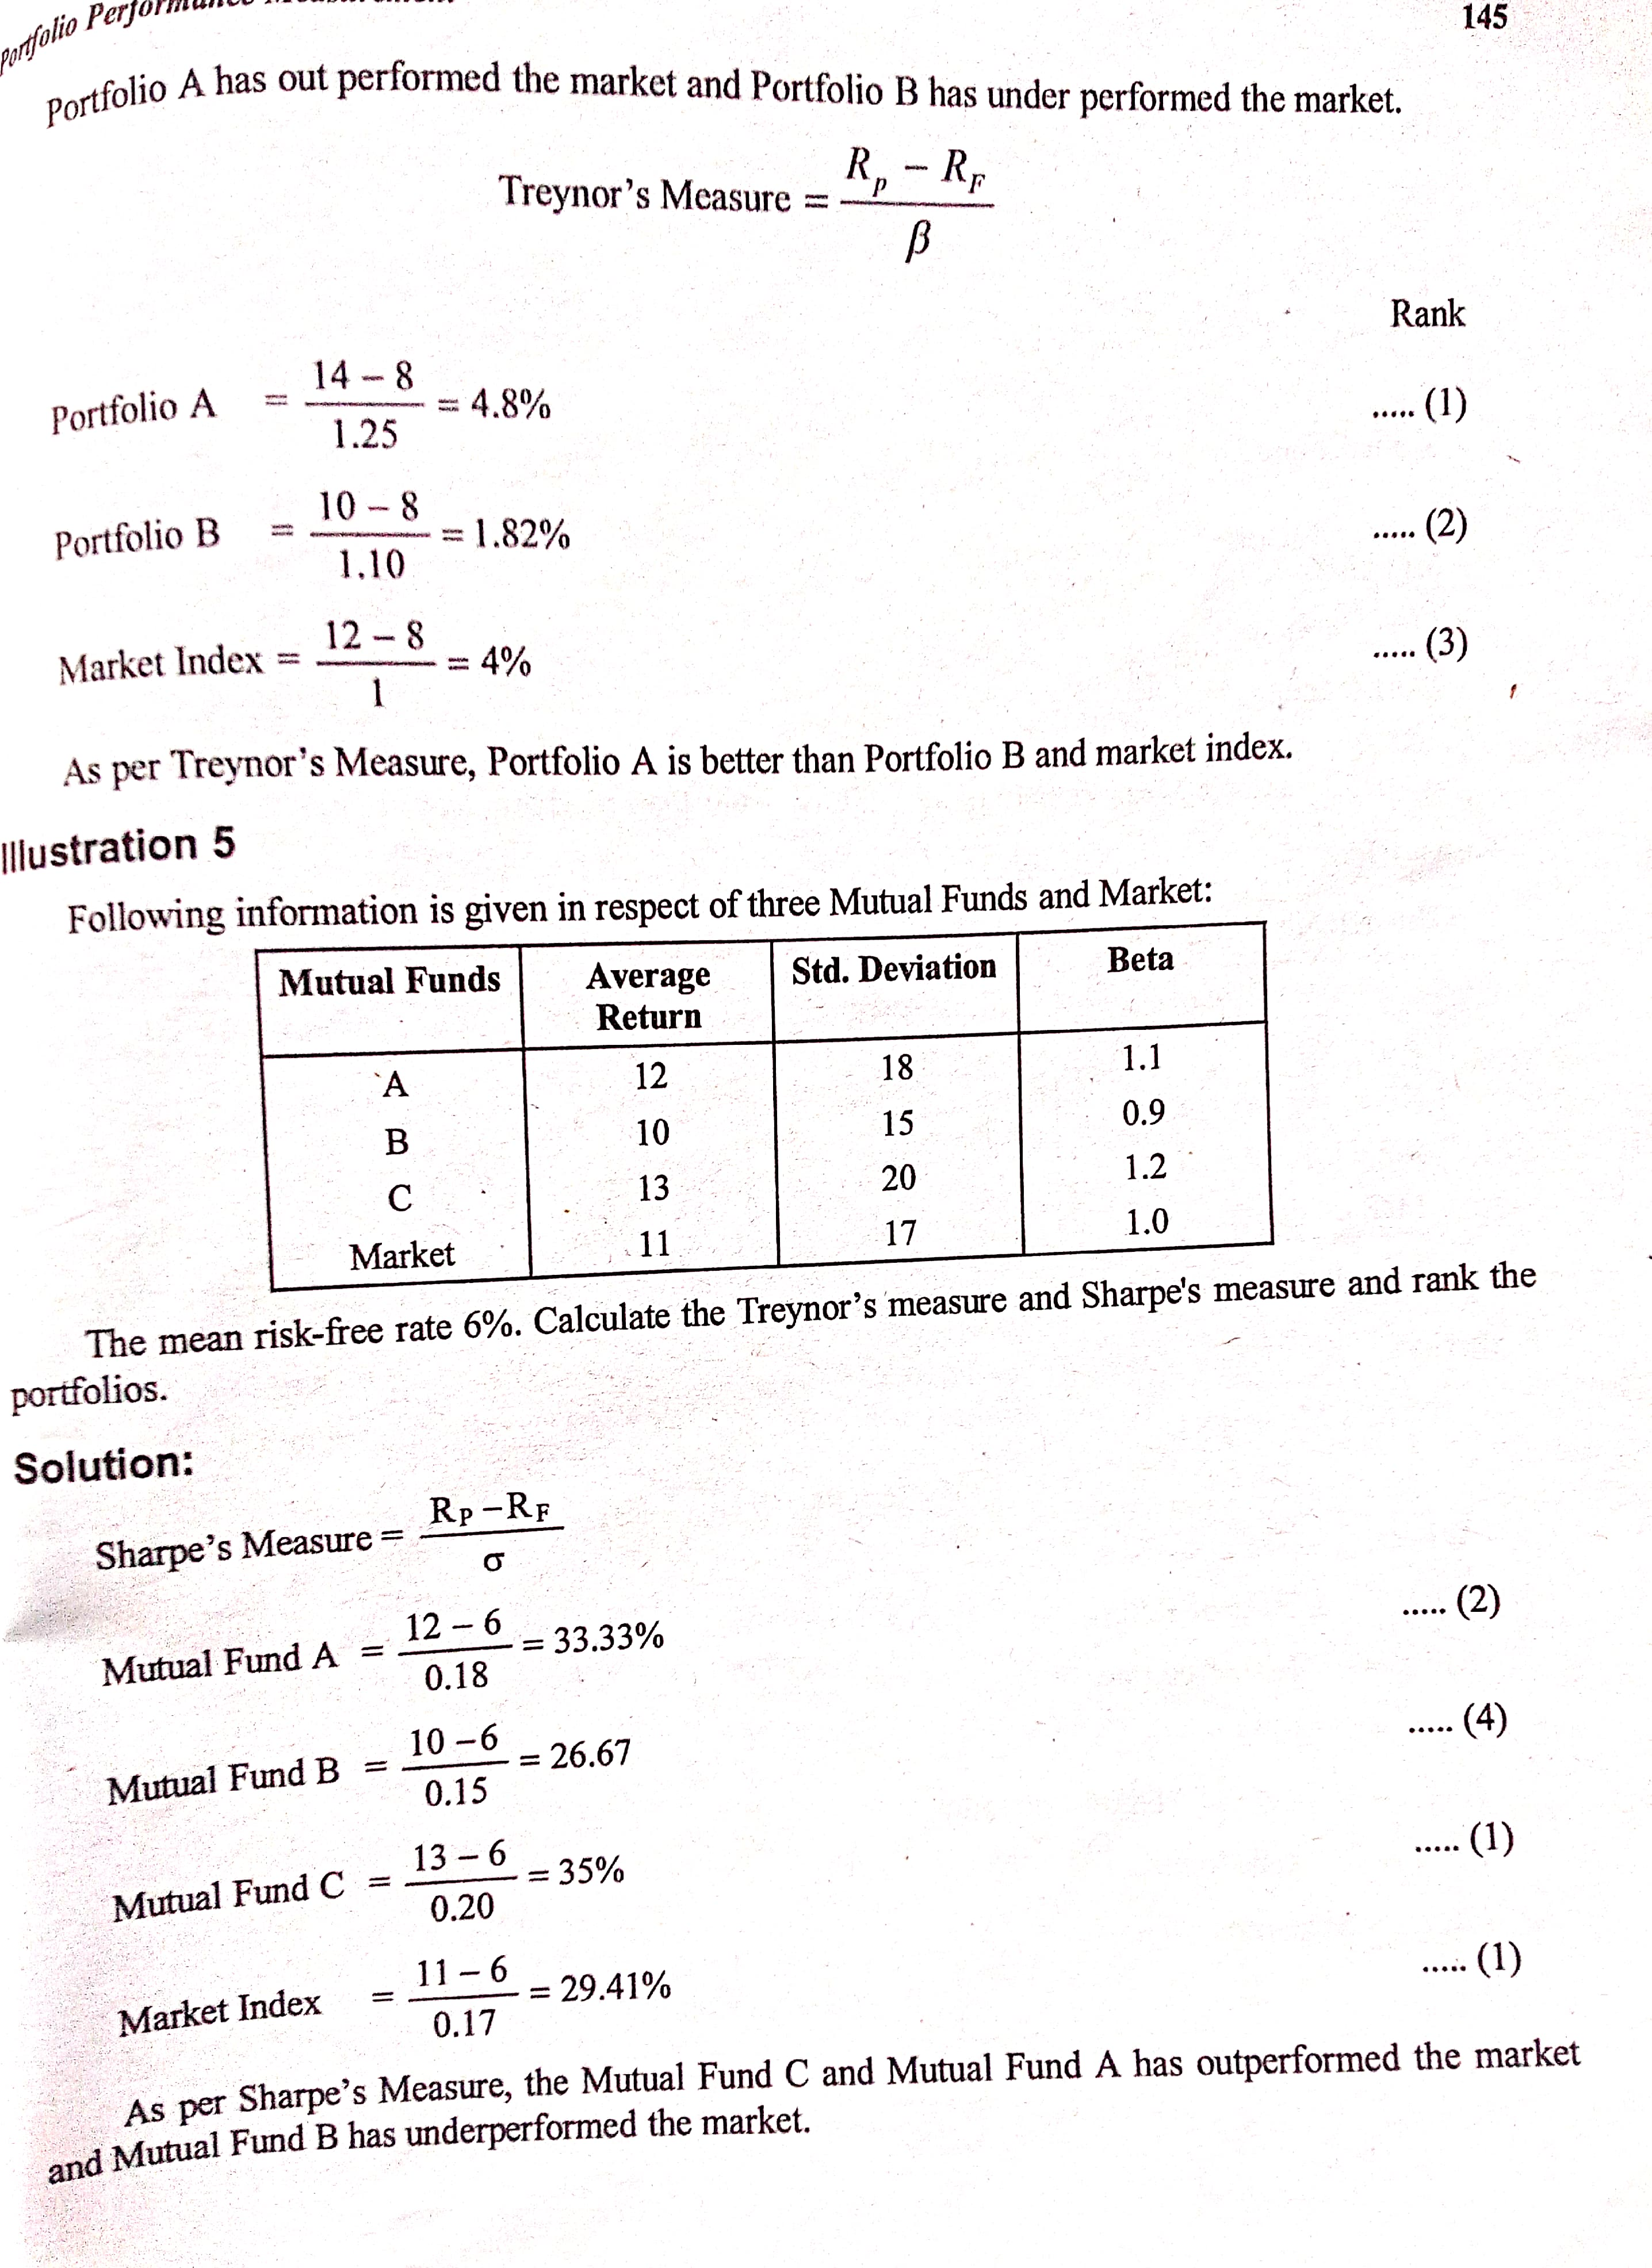
\includegraphics{figures/fig_0096.jpeg}
\textgreater{} OCR cue: 1io0 A has out performed t 145 postfo P ned the
market and Portfolio B has under performed the mark \textbar{} ae e
market. Treynor's Measure = Ky 7 Re i Rank portfolio A = `` = = 4.8\%
Cees ei. eC cr a ra (1) Portfolio B = 10-8 = 1.82\% TAOce er ne otek ee
pe ee. iceman eG te (2) Market Index = 1278 . gy, 1 sO ae (3) As per
Treynor's Measure, Portfolio A is better than Portfolio B and market
'dex: illustrati

\hypertarget{figure-3-page-3-1}{%
\subsubsection{Figure 3 (Page 3)}\label{figure-3-page-3-1}}

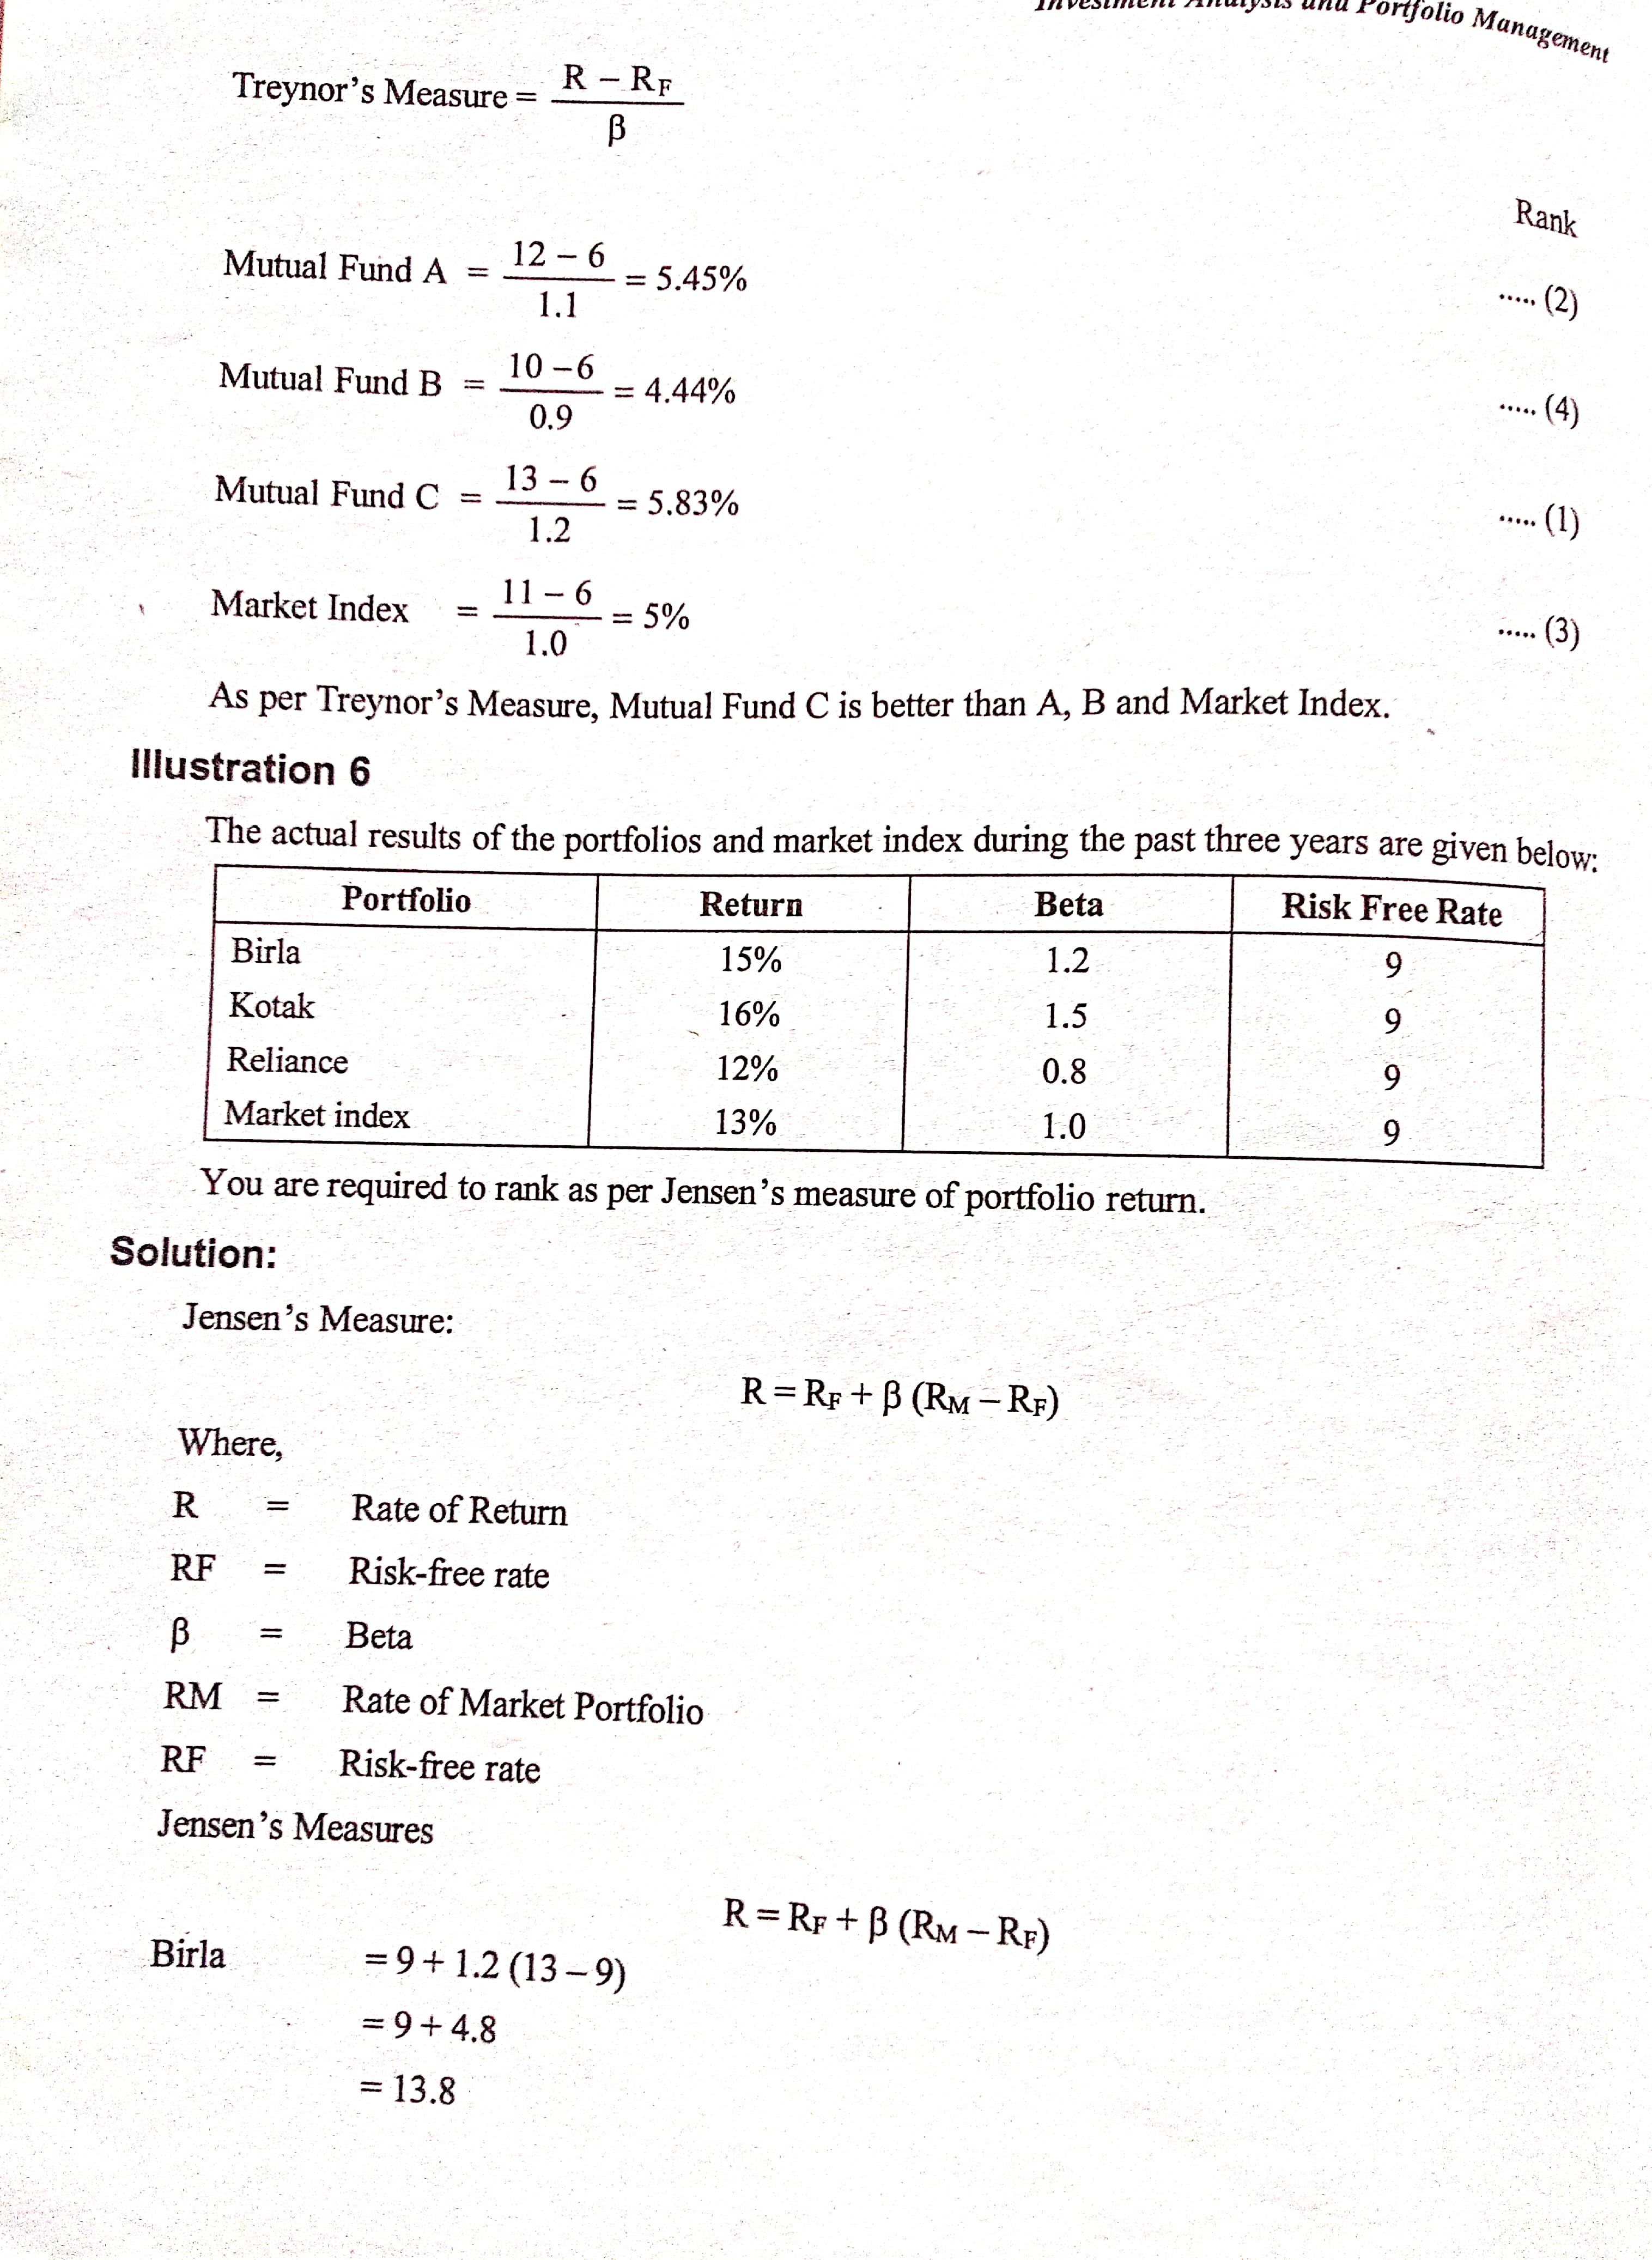
\includegraphics{figures/fig_0097.jpeg}
\textgreater{} OCR cue: BLE VOCOESIERTEE £BEENOE TED SIEM t OFtfolig Ma
Treynor's Measure sr Rank ) \textbar{} 4126 Mutual Fund A = --- SRO BS
ata wg te a Sane \& Fae (2) : \_ 10-6 Mutual FundB=------'' 24.44\% (4)
0.9 13 ---6 Mutual Fund C = Tad DR A Cee ent ert (1) : 11-6 Market Index
= 7 SO Pg gitar.'' Bh Re, oe eee sels ee (3) As per Treynor's Measure,
Mutual Fund C is better than A, B and Market Index. illustration 6 The
actual results o

\hypertarget{figure-4-page-4-1}{%
\subsubsection{Figure 4 (Page 4)}\label{figure-4-page-4-1}}

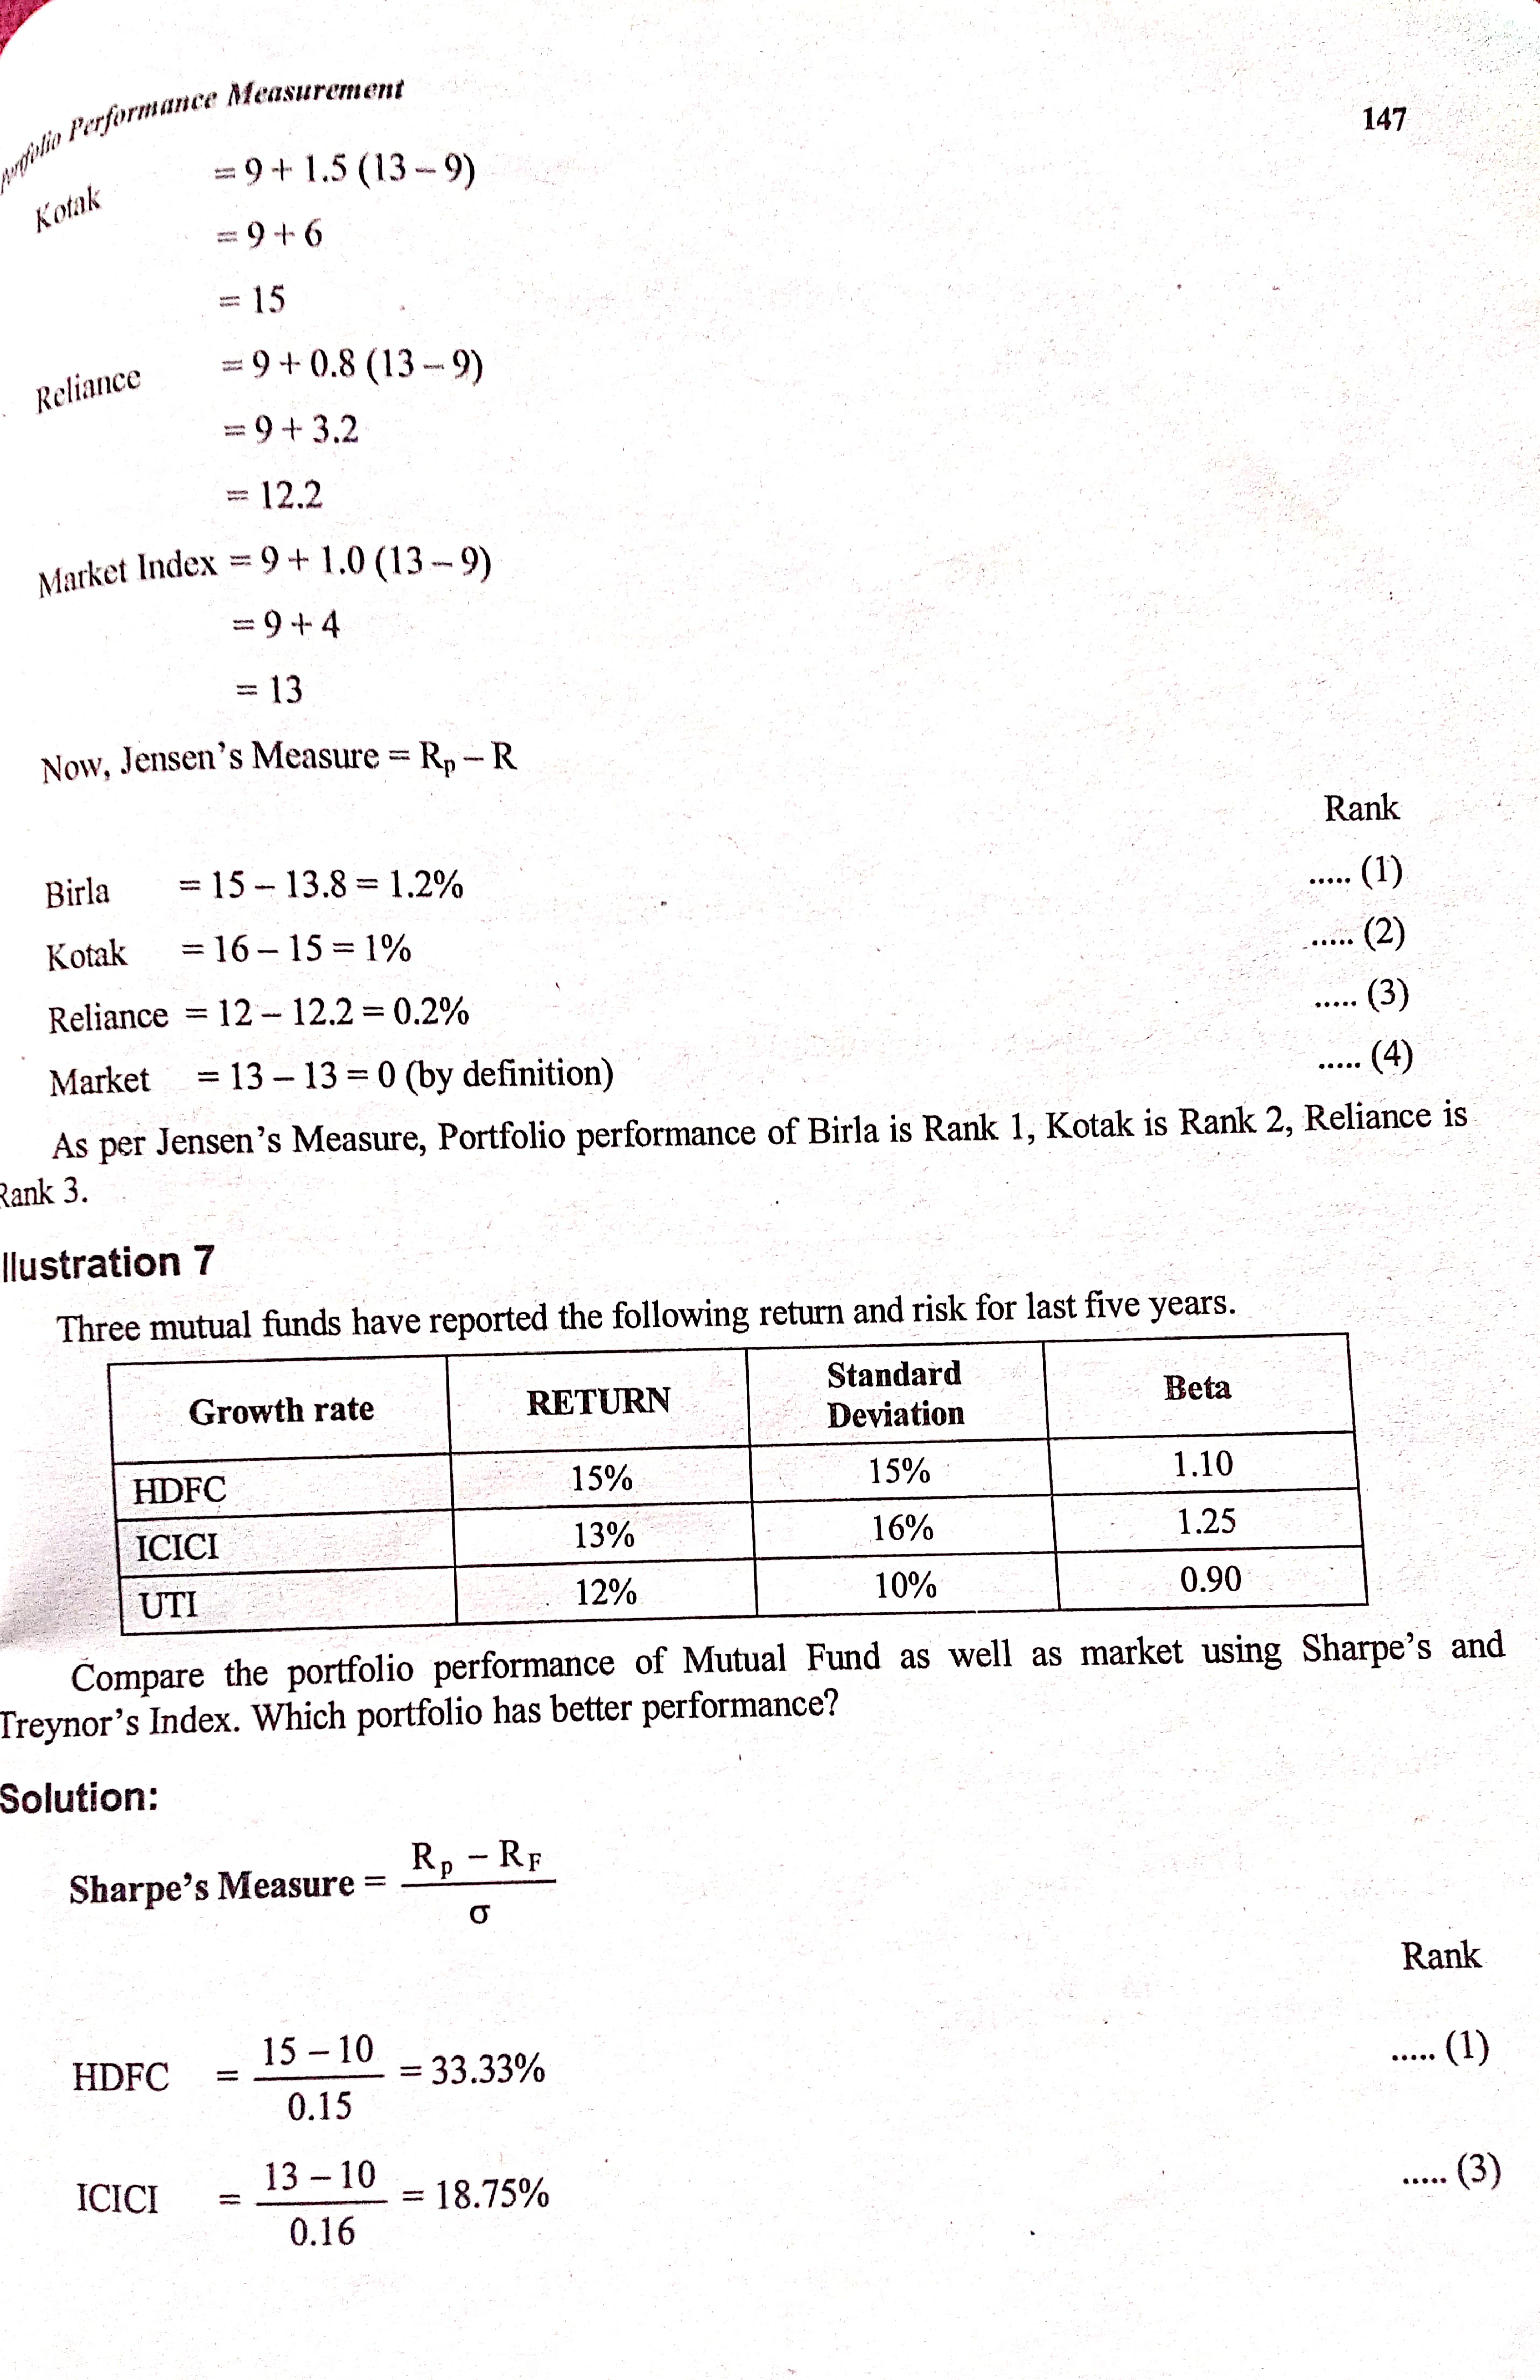
\includegraphics{figures/fig_0098.jpeg}
\textgreater{} OCR cue: y 7) vasurement '' pf Ad Afe 1'' perfor 147 iil
=9+1.5 (13-9) cotitk . =O+6 = 15 \textbar{} reliance =9+0.8 (13-9)
=9+3.2 = 12.2 Market Index = 9 + 1.0 (13 ---9) =9+4 =13 Now, Jensen's
Measure = Rp --- R Rank pirla = = 15-13.8=12\% \_ peta eat: (1) Kotak
=16-15=1\% \textbar{} ue) Reliance =12----12.2=0.2\% ES a (3). Market
=13---13=0 (by definition) 3 \textbar{} ah ee he ae (4) As per Jensen's
Measure, Portfolio performance of Birla is R

\hypertarget{figure-5-page-5-1}{%
\subsubsection{Figure 5 (Page 5)}\label{figure-5-page-5-1}}

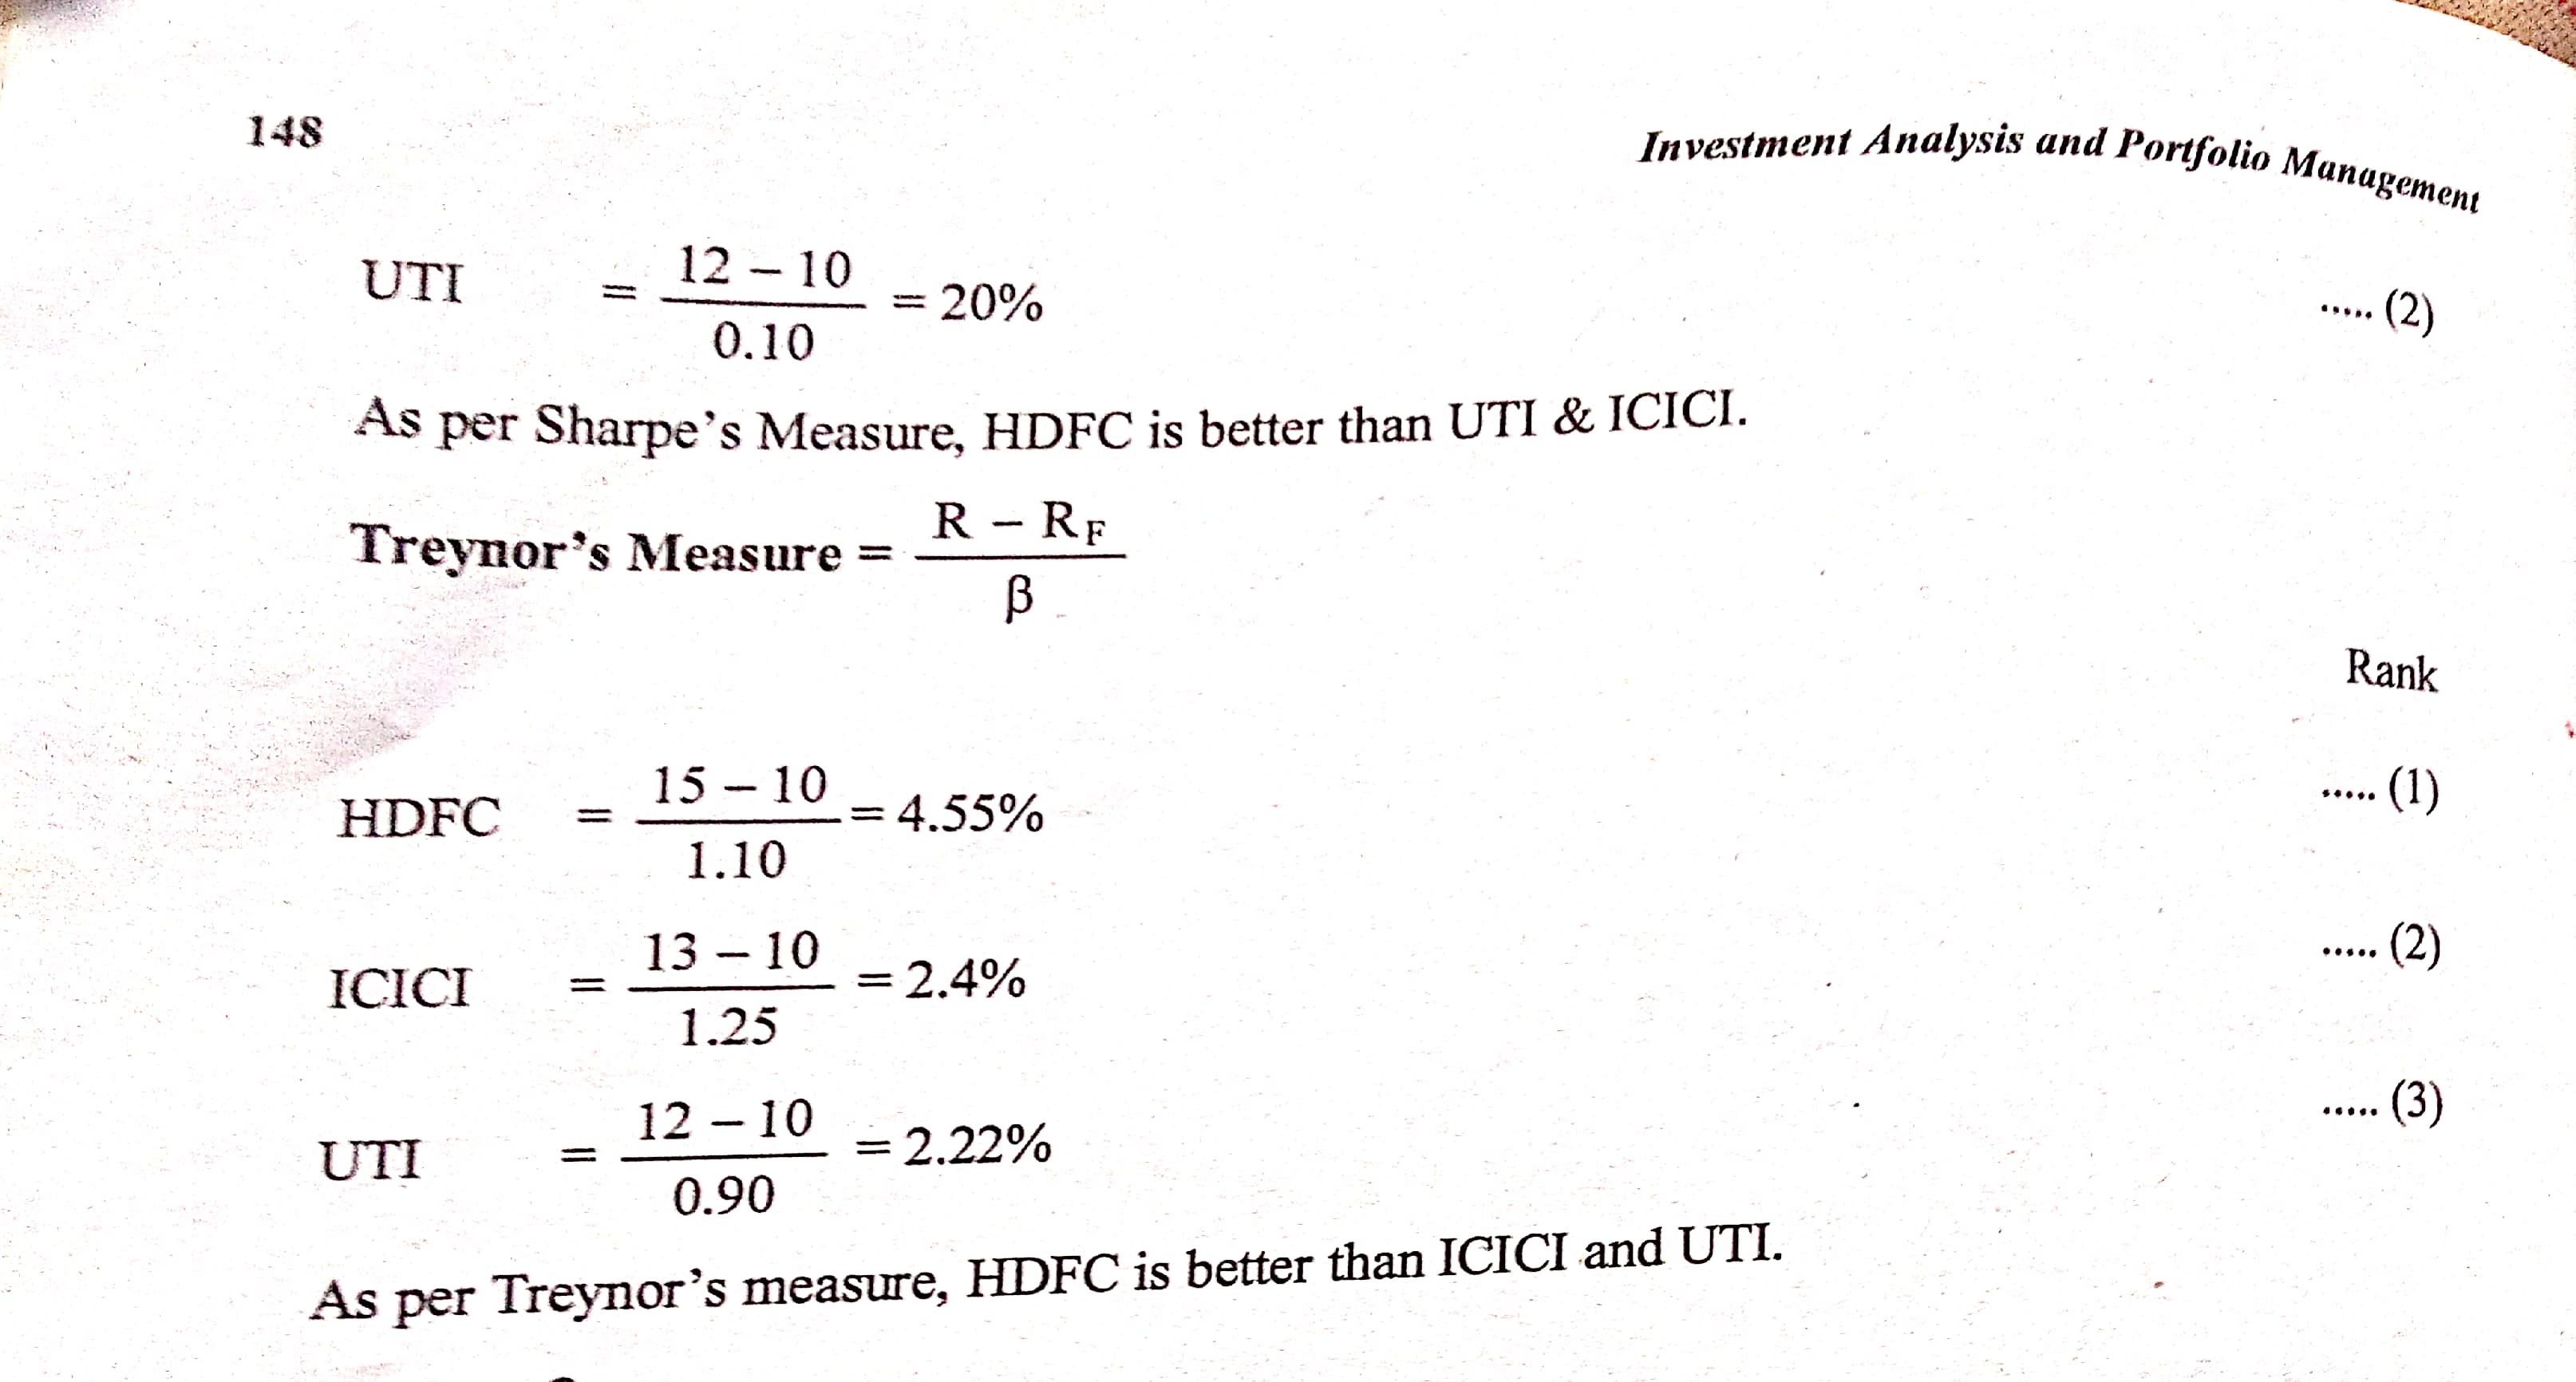
\includegraphics{figures/fig_0099.jpeg}
\textgreater{} OCR cue: 148 Investment Analysis and Portfolig Managen
eheny 9 te TO tae 0.10 nee \textbar{} vv (2) As per Sharpe's Measure,
HDFC is better than UTI \& ICICI. Treynor's Measure = SBE. B Rank HDFC =
a = 4.55\% di. (1) ICICI = a oy igs ee aE Rag a eh ge Ep (2) \$F TO oSee
BO es ET et peg Es oor (3) x. Ss 9M 0.90 As per Treynor's measure, HDEC
is better than ICICI and UTI.

\hypertarget{unit-63-foreign-exchange-risk.pdf}{%
\subsection{UNIT 6/3 Foreign Exchange
Risk.pdf}\label{unit-63-foreign-exchange-risk.pdf}}

\hypertarget{figure-1-page-1-2}{%
\subsubsection{Figure 1 (Page 1)}\label{figure-1-page-1-2}}

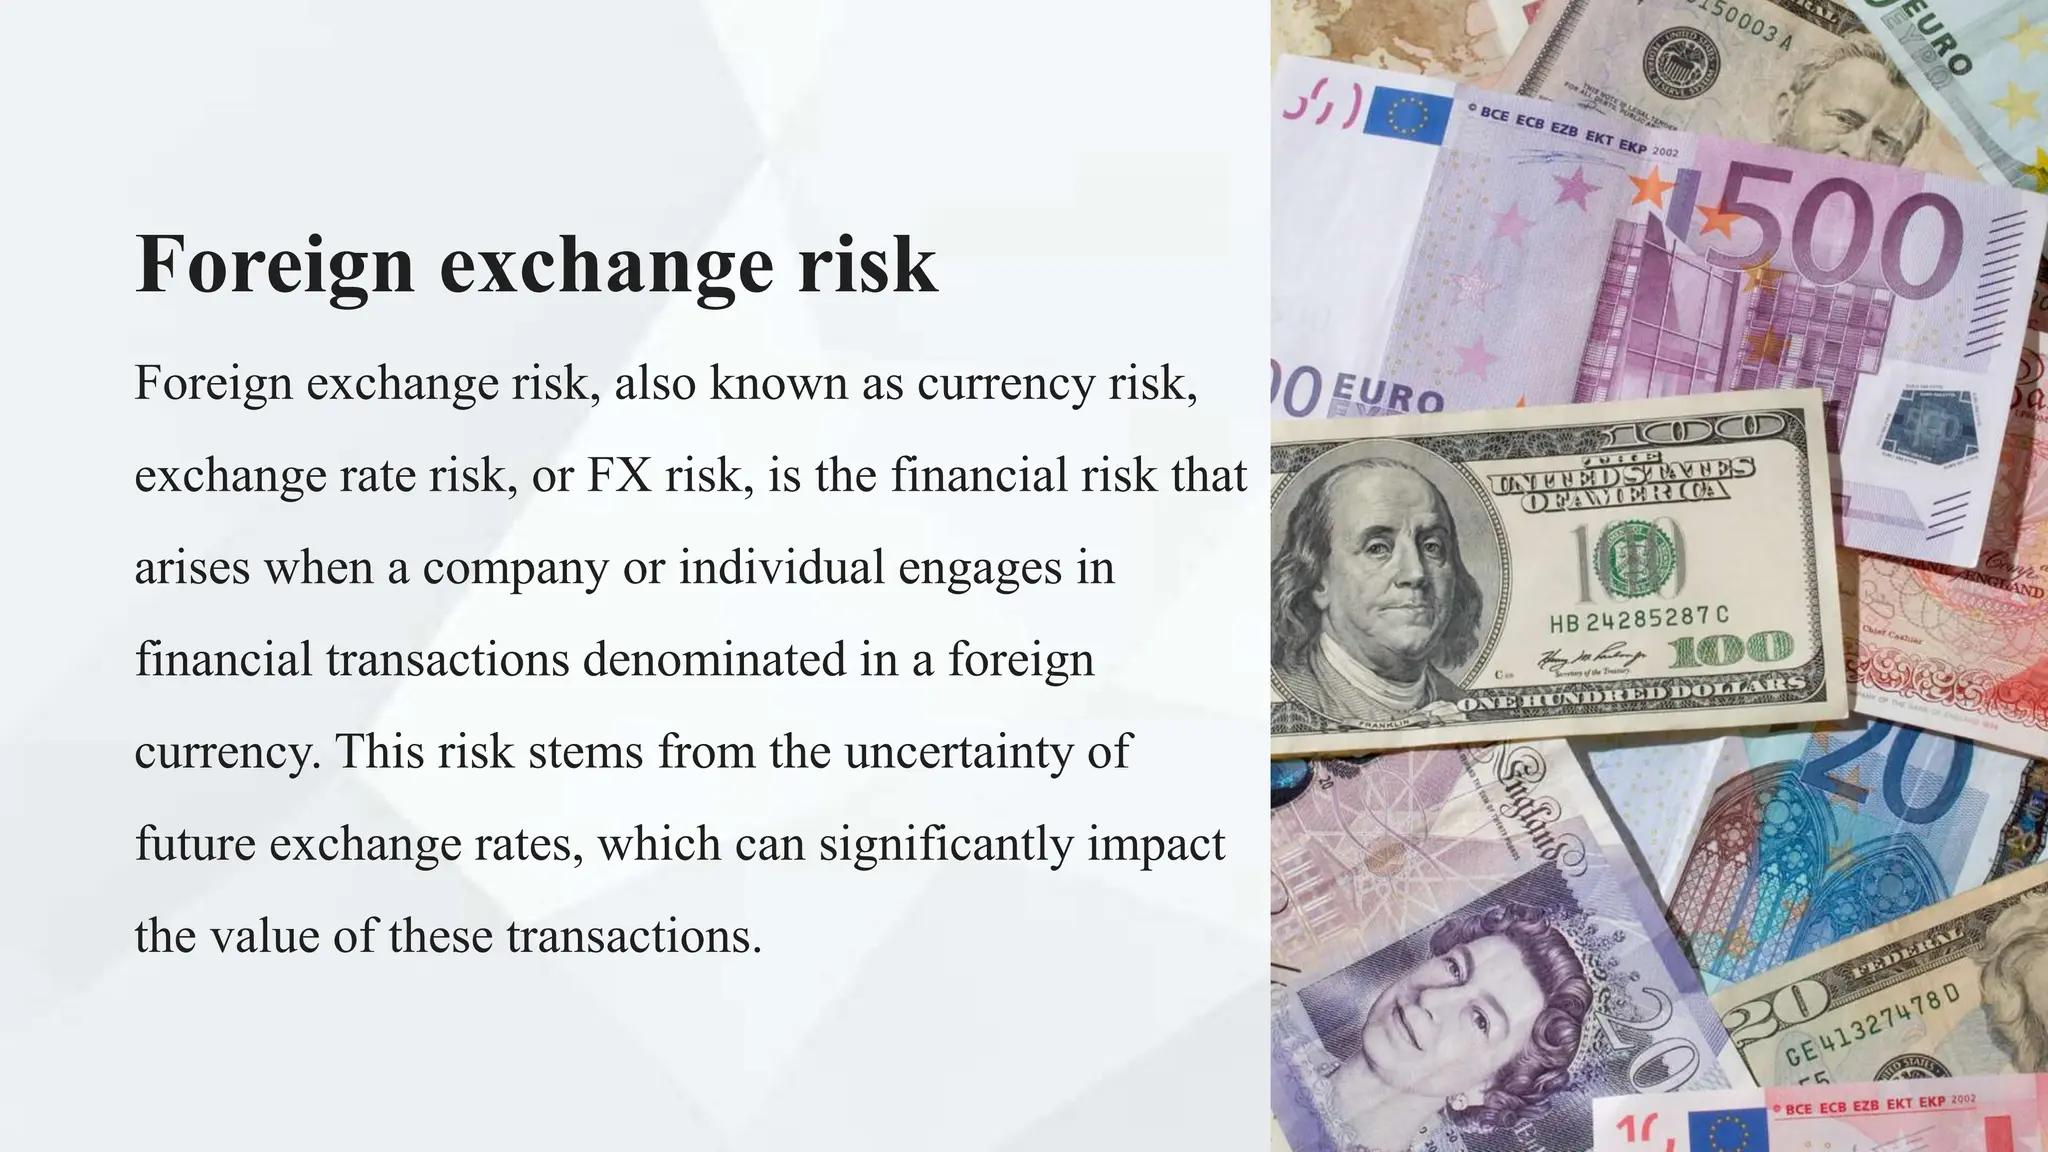
\includegraphics{figures/fig_0100.jpeg}
\textgreater{} OCR cue: Foreign exchange risk Foreign exchange risk,
also known as currency risk, exchange rate risk, or FX risk, is the
financial risk that ; arises when a company or individual engages in
financial transactions denominated in a foreign currency. This risk
stems from the uncertainty of future exchange rates, which can
significantly impact the value of these transactions.

\hypertarget{figure-2-page-2-2}{%
\subsubsection{Figure 2 (Page 2)}\label{figure-2-page-2-2}}

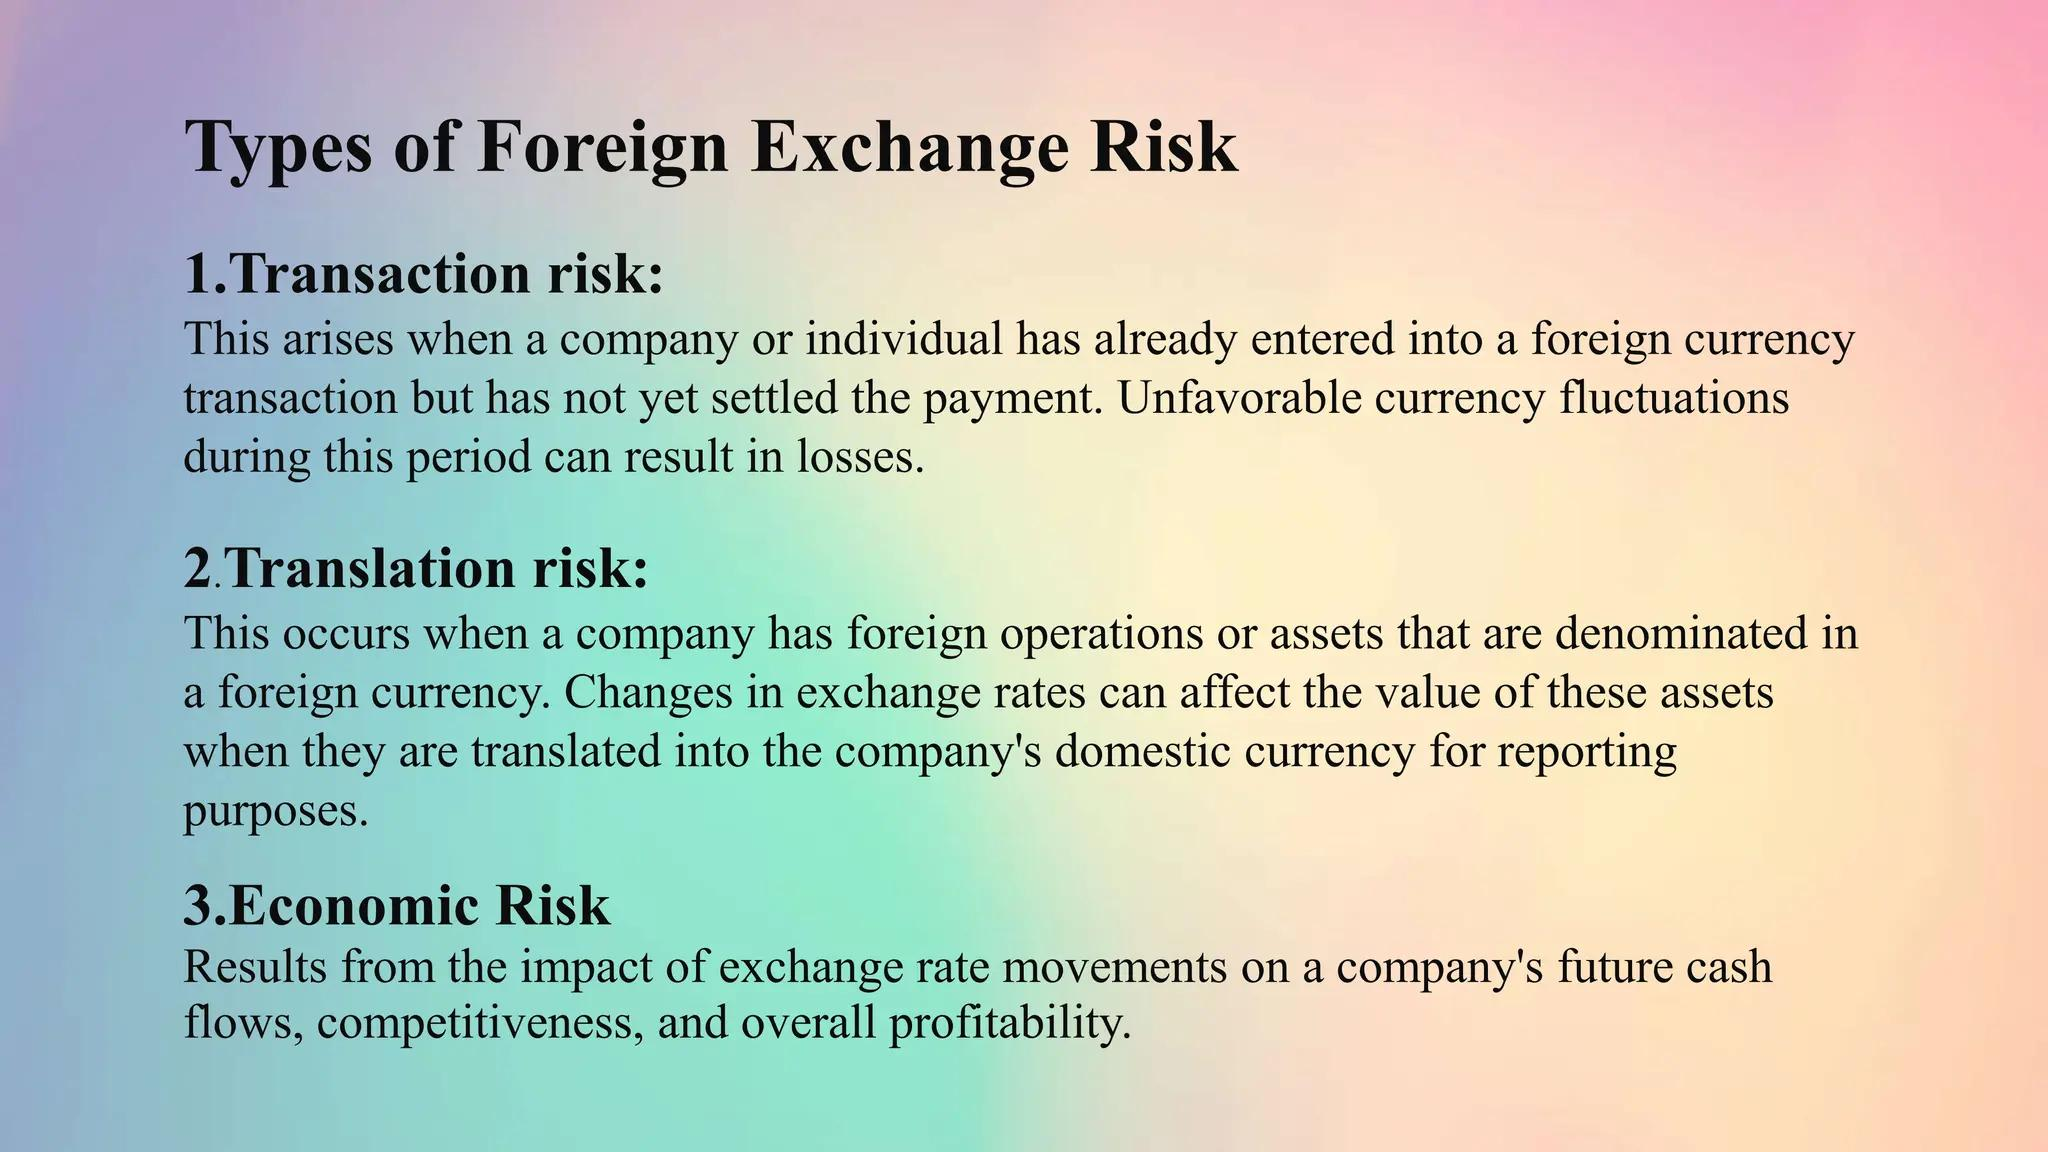
\includegraphics{figures/fig_0101.jpeg}
\textgreater{} OCR cue: Types of Foreign Exchange Risk 1.Transaction
risk: This arises when a company or individual has already entered into
a foreign currency transaction but has not yet settled the payment.
Unfavorable currency fluctuations during this period can result in
losses. 2.Translation risk: This occurs when a company has foreign
operations or assets that are denominated in a foreign currency. Changes
in excha

\hypertarget{figure-3-page-6}{%
\subsubsection{Figure 3 (Page 6)}\label{figure-3-page-6}}

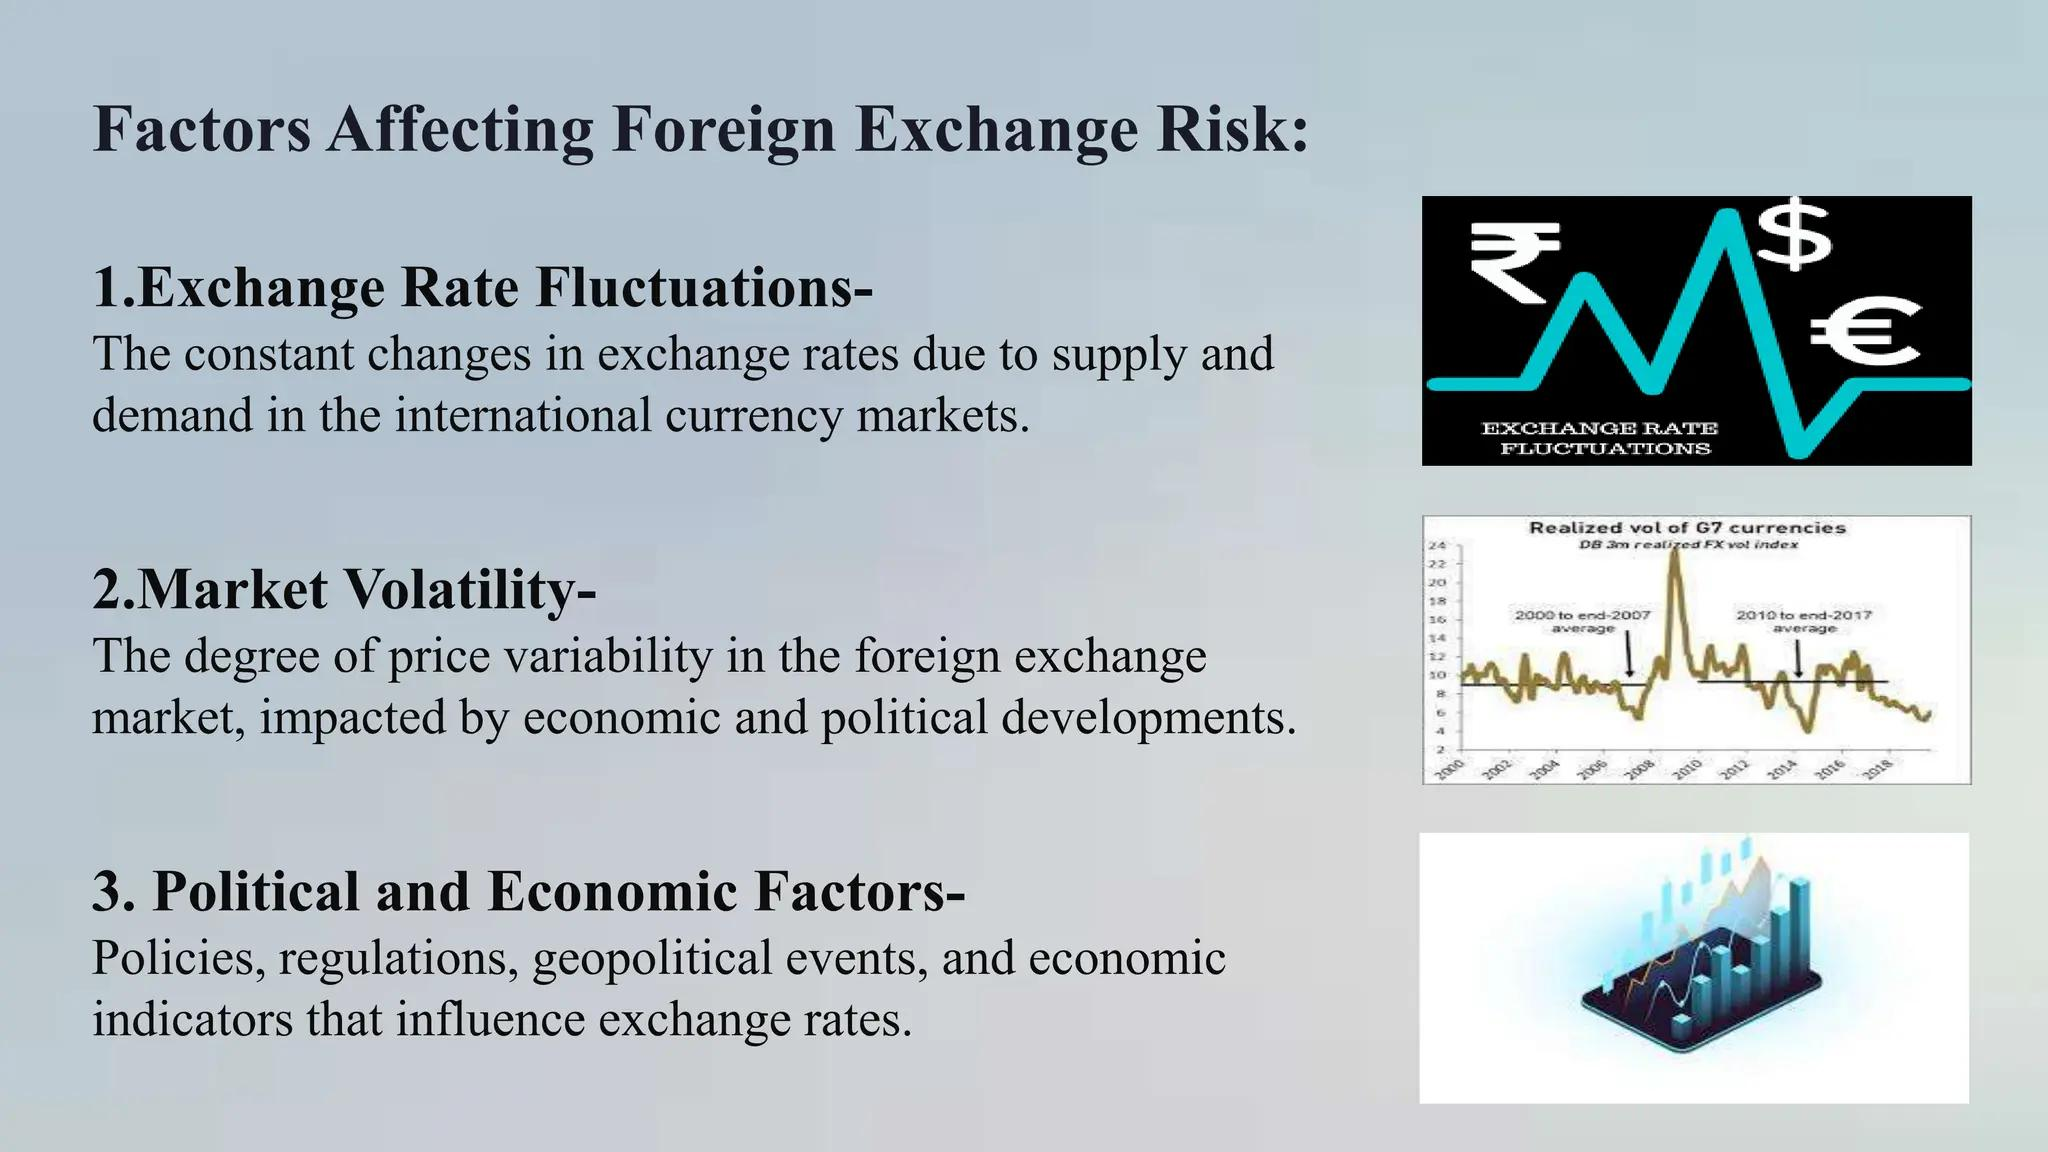
\includegraphics{figures/fig_0102.jpeg}
\textgreater{} OCR cue: Factors Affecting Foreign Exchange Risk:
1.Exchange Rate Fluctuations- \textless= The constant changes in
exchange rates due to supply and demand in the international currency
markets. EXCHANGE RATE FLUCTUATIONS Realized vol of G7 28 3m realized FX
vot 2.Market Volatility- The degree of price variability in the foreign
exchange market, impacted by economic and political developments. 3.
Political and Econ

\hypertarget{figure-4-page-7}{%
\subsubsection{Figure 4 (Page 7)}\label{figure-4-page-7}}

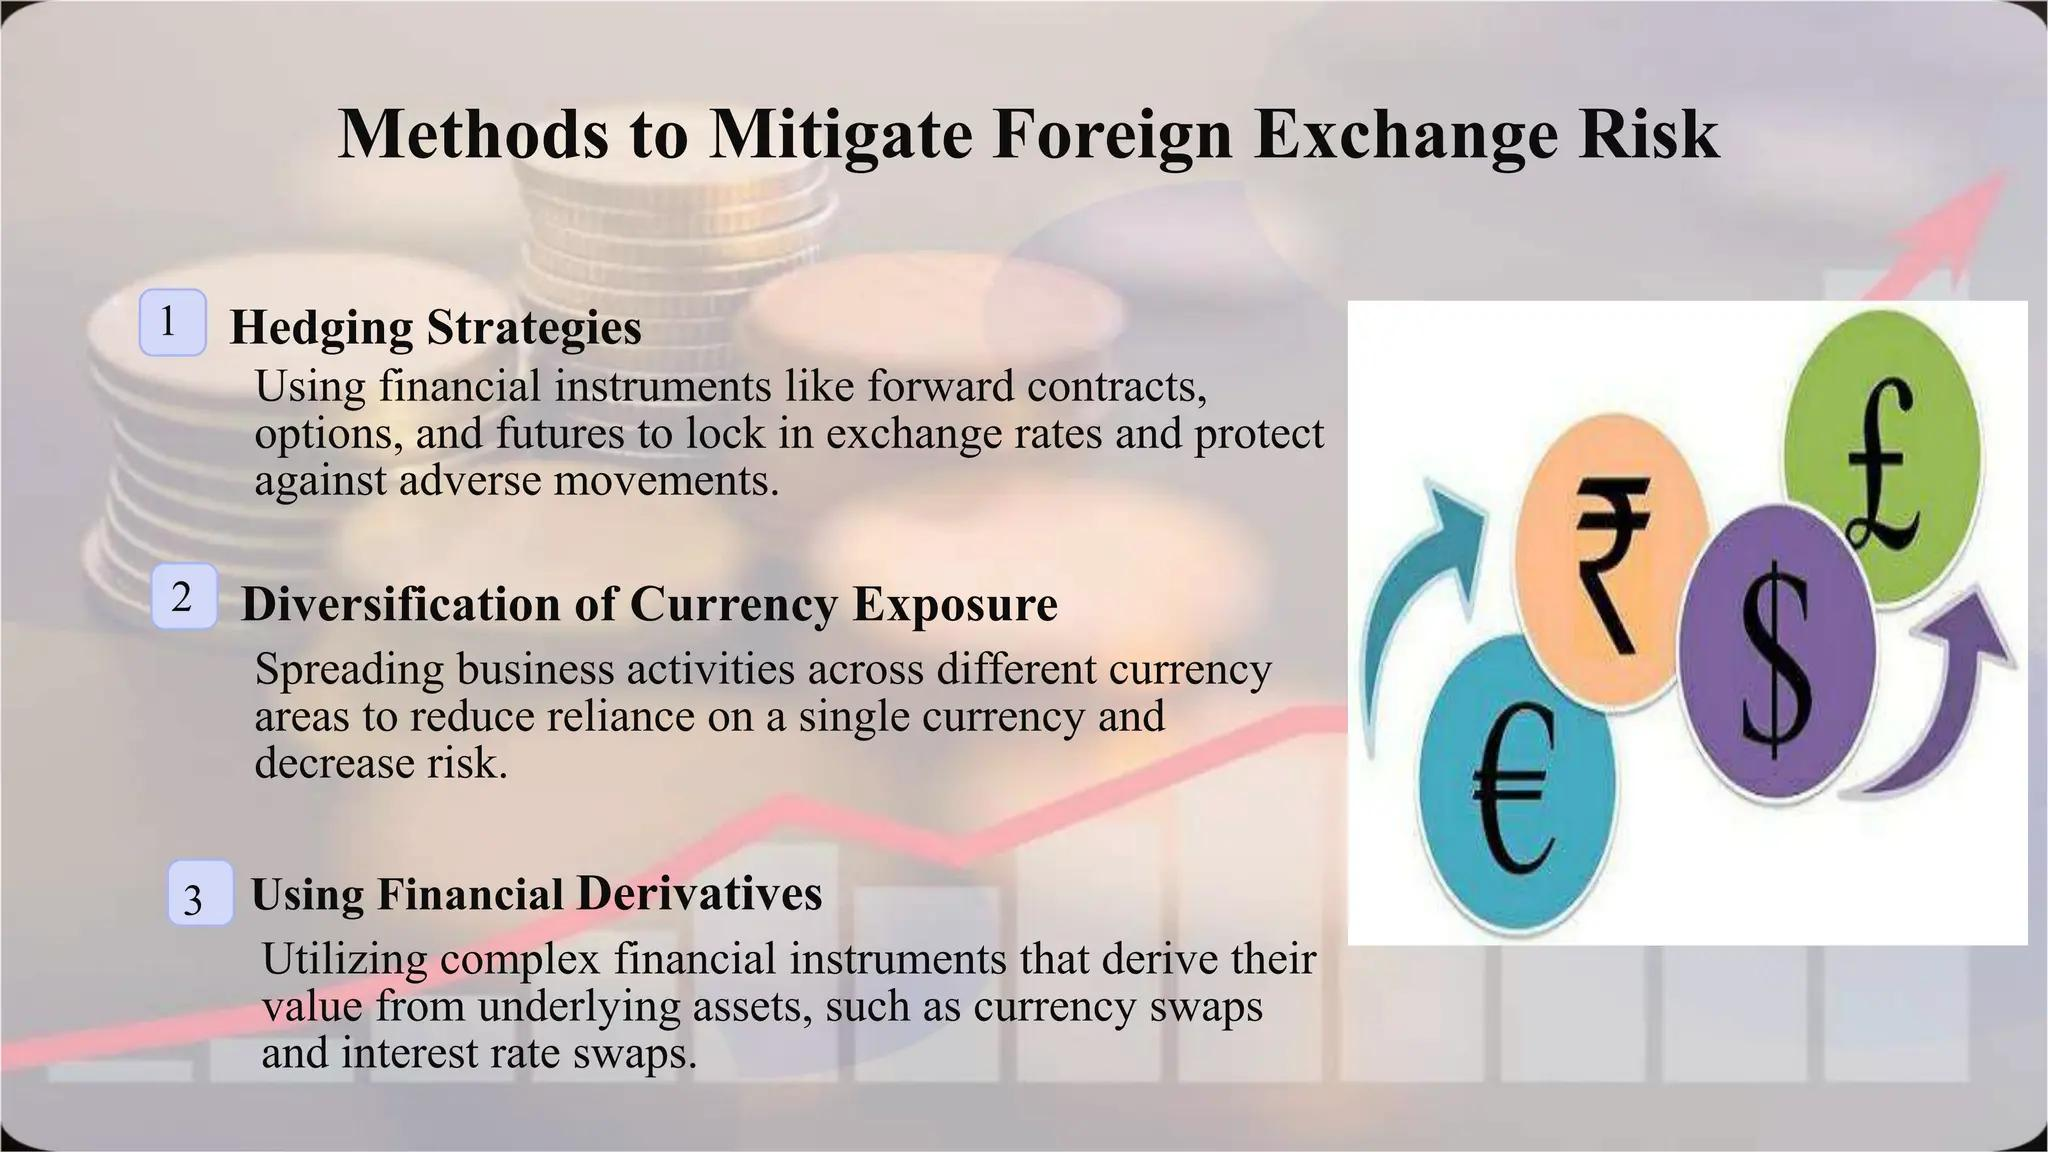
\includegraphics{figures/fig_0103.jpeg}
\textgreater{} OCR cue: Methods to Mitigate Foreign Exchange Risk 1
Hedging Strategies Using financial instruments like forward contracts,
options, and futures to lock in exchange rates and protect against
adverse movements. 2 Diversification of Currency Exposure Spreading
business activities across different currency areas to reduce reliance
on a single currency and decrease risk. 3. Using Financial Derivatives
Utilizin

\hypertarget{figure-5-page-8}{%
\subsubsection{Figure 5 (Page 8)}\label{figure-5-page-8}}

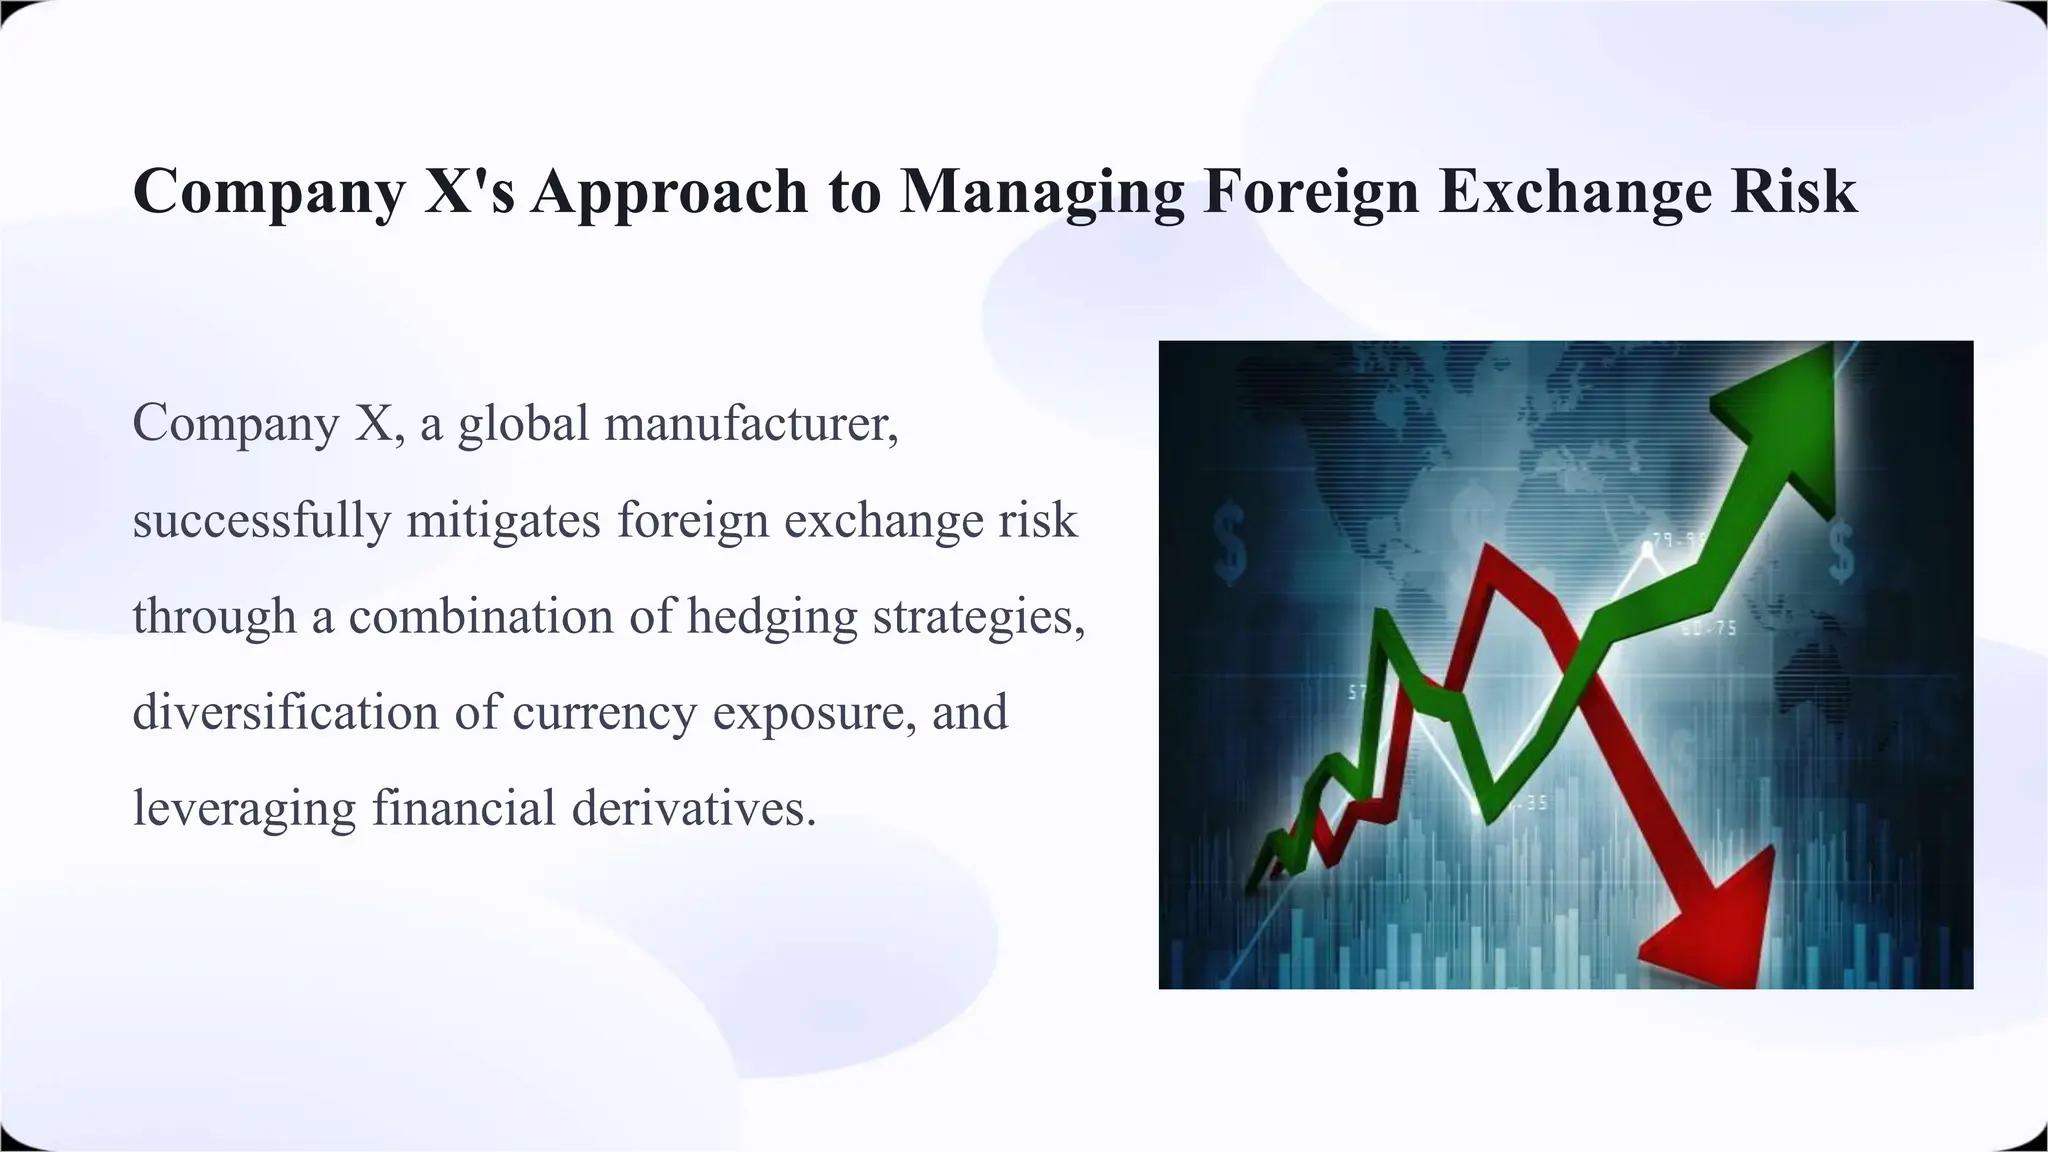
\includegraphics{figures/fig_0104.jpeg}
\textgreater{} OCR cue: Company X's Approach to Managing Foreign
Exchange Risk Company X, a global manufacturer, successfully mitigates
foreign exchange risk through a combination of hedging strategies,
diversification of currency exposure, and leveraging financial
derivatives.

\hypertarget{figure-6-page-9}{%
\subsubsection{Figure 6 (Page 9)}\label{figure-6-page-9}}

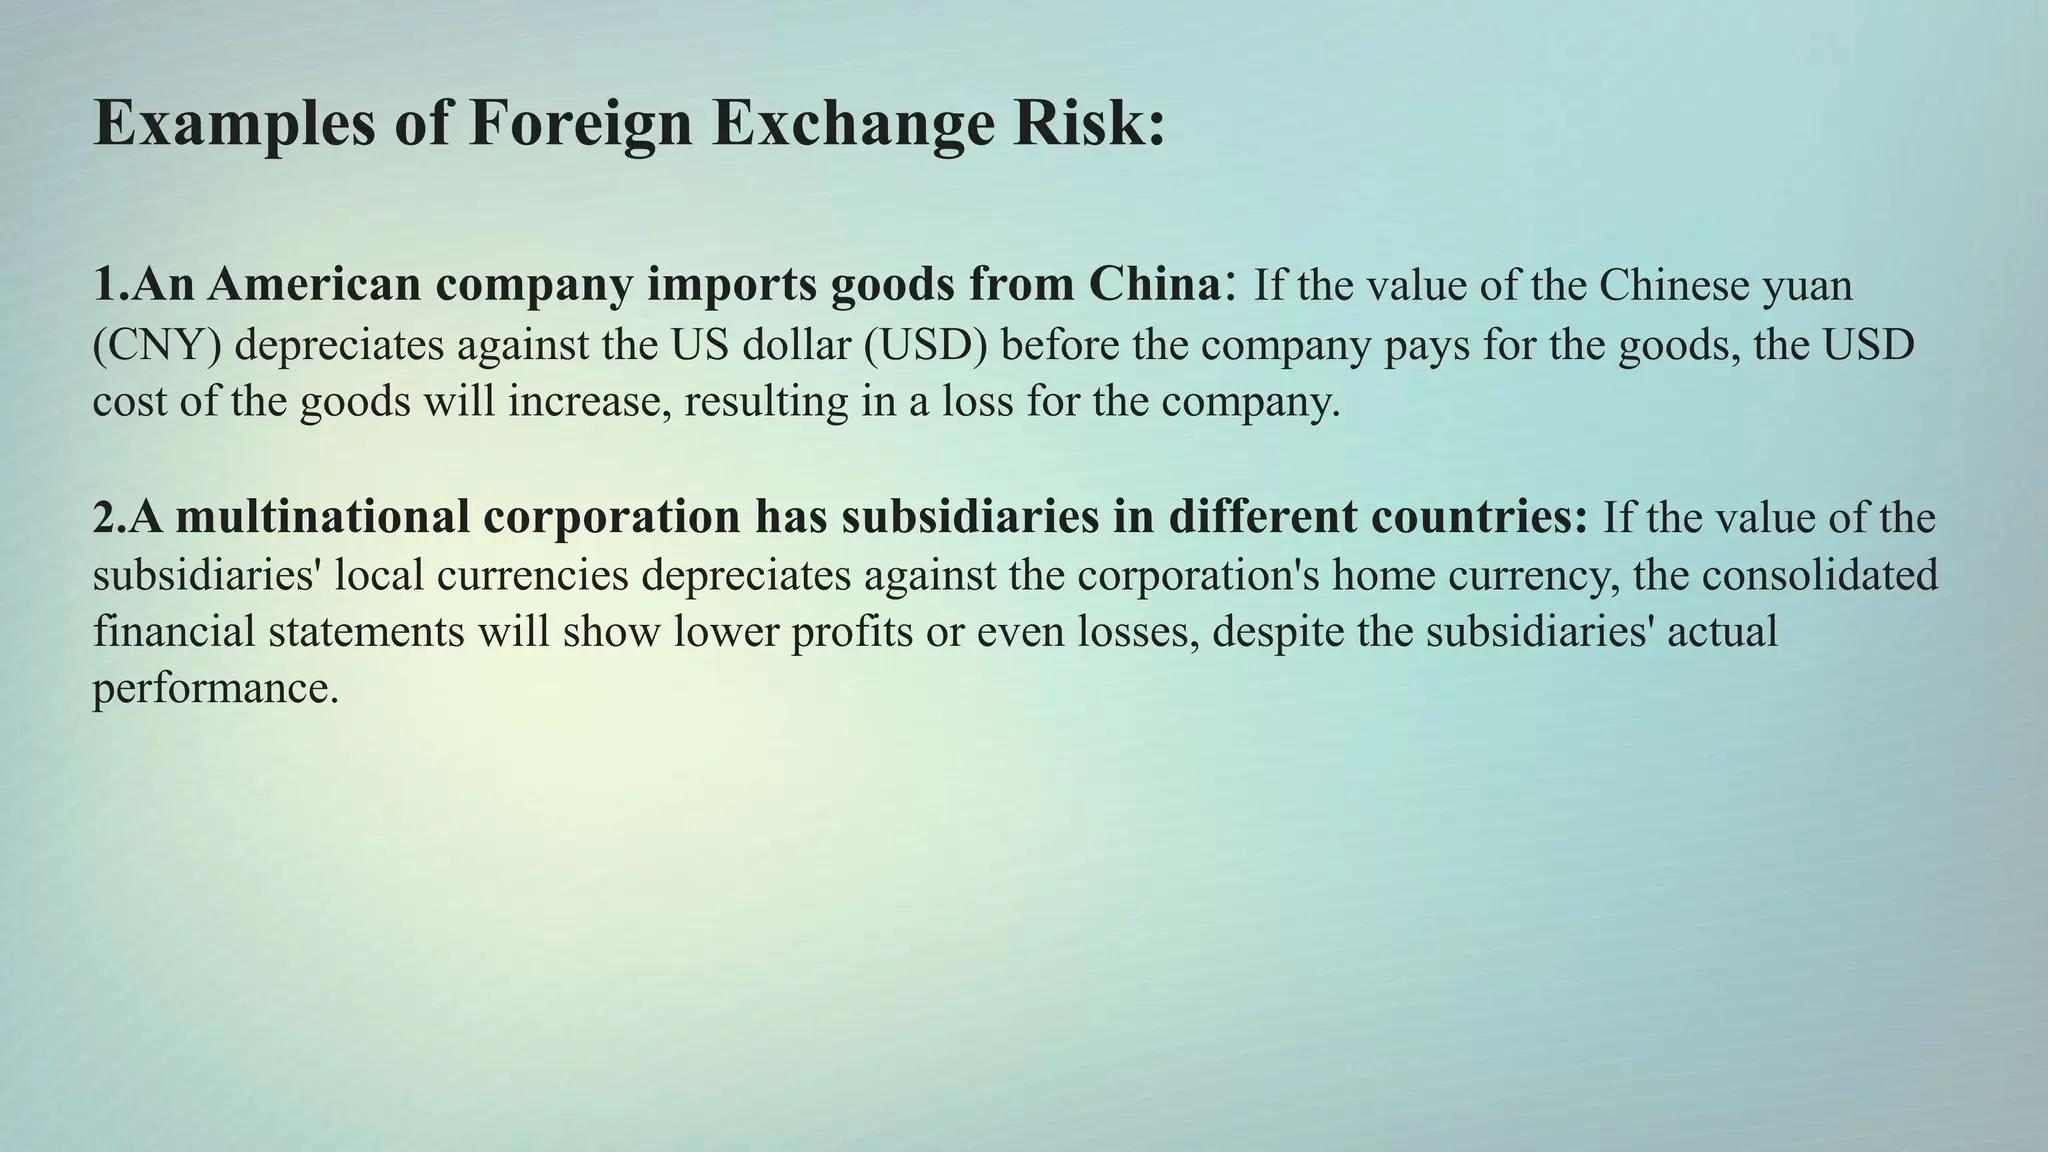
\includegraphics{figures/fig_0105.jpeg}
\textgreater{} OCR cue: Examples of Foreign Exchange Risk: 1.An American
company imports goods from China: If the value of the Chinese yuan (CNY)
depreciates against the US dollar (USD) before the company pays for the
goods, the USD cost of the goods will increase, resulting in a loss for
the company. 2.A multinational corporation has subsidiaries in different
countries: If the value of the subsidiaries' local currencies

\hypertarget{figure-7-page-10}{%
\subsubsection{Figure 7 (Page 10)}\label{figure-7-page-10}}

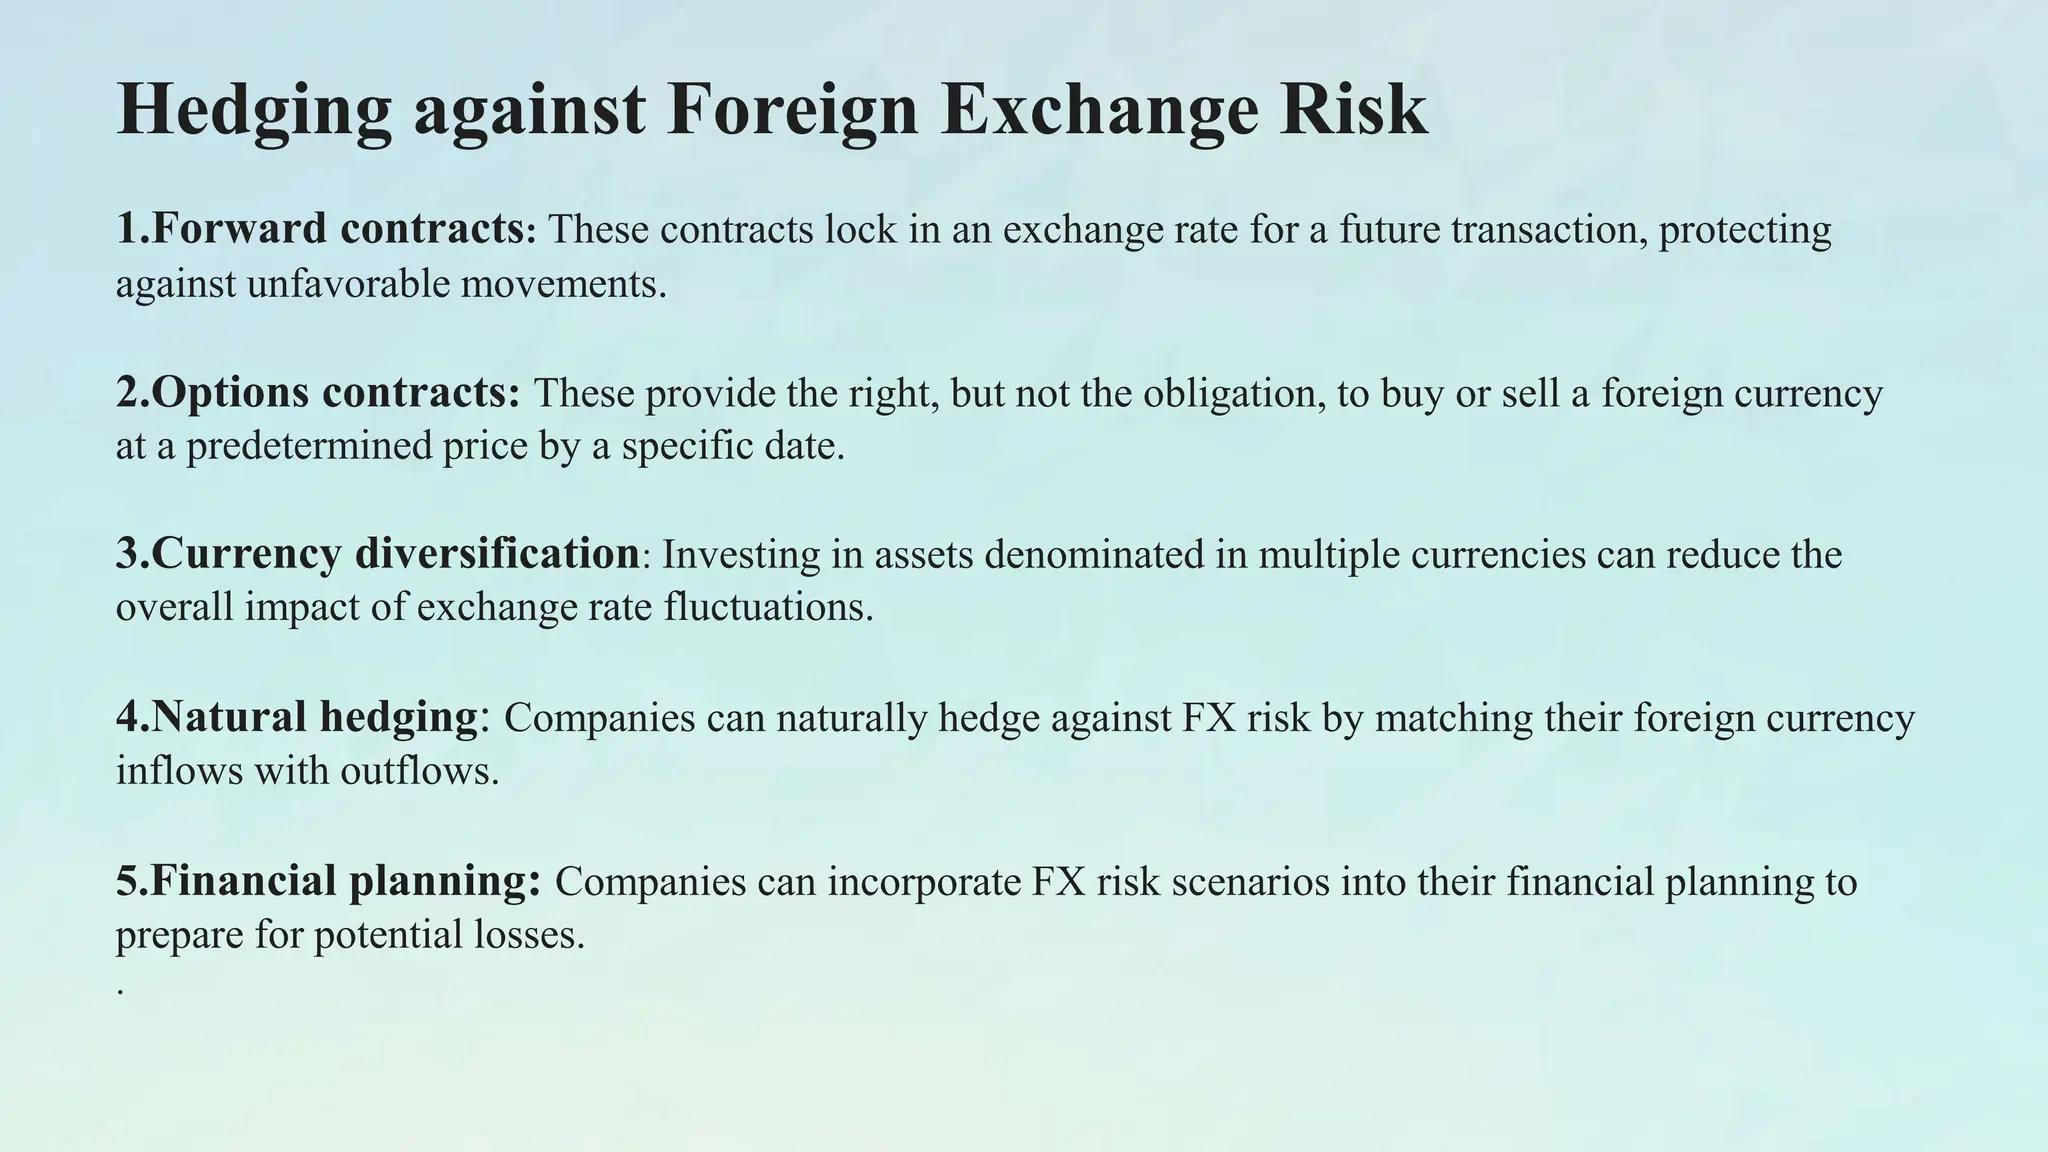
\includegraphics{figures/fig_0106.jpeg}
\textgreater{} OCR cue: Hedging against Foreign Exchange Risk 1.Forward
contracts: These contracts lock in an exchange rate for a future
transaction, protecting against unfavorable movements. 2.Options
contracts: These provide the right, but not the obligation, to buy or
sell a foreign currency at a predetermined price by a specific date.
3.Currency diversification: Investing in assets denominated in multiple
currencies

\hypertarget{figure-8-page-11}{%
\subsubsection{Figure 8 (Page 11)}\label{figure-8-page-11}}

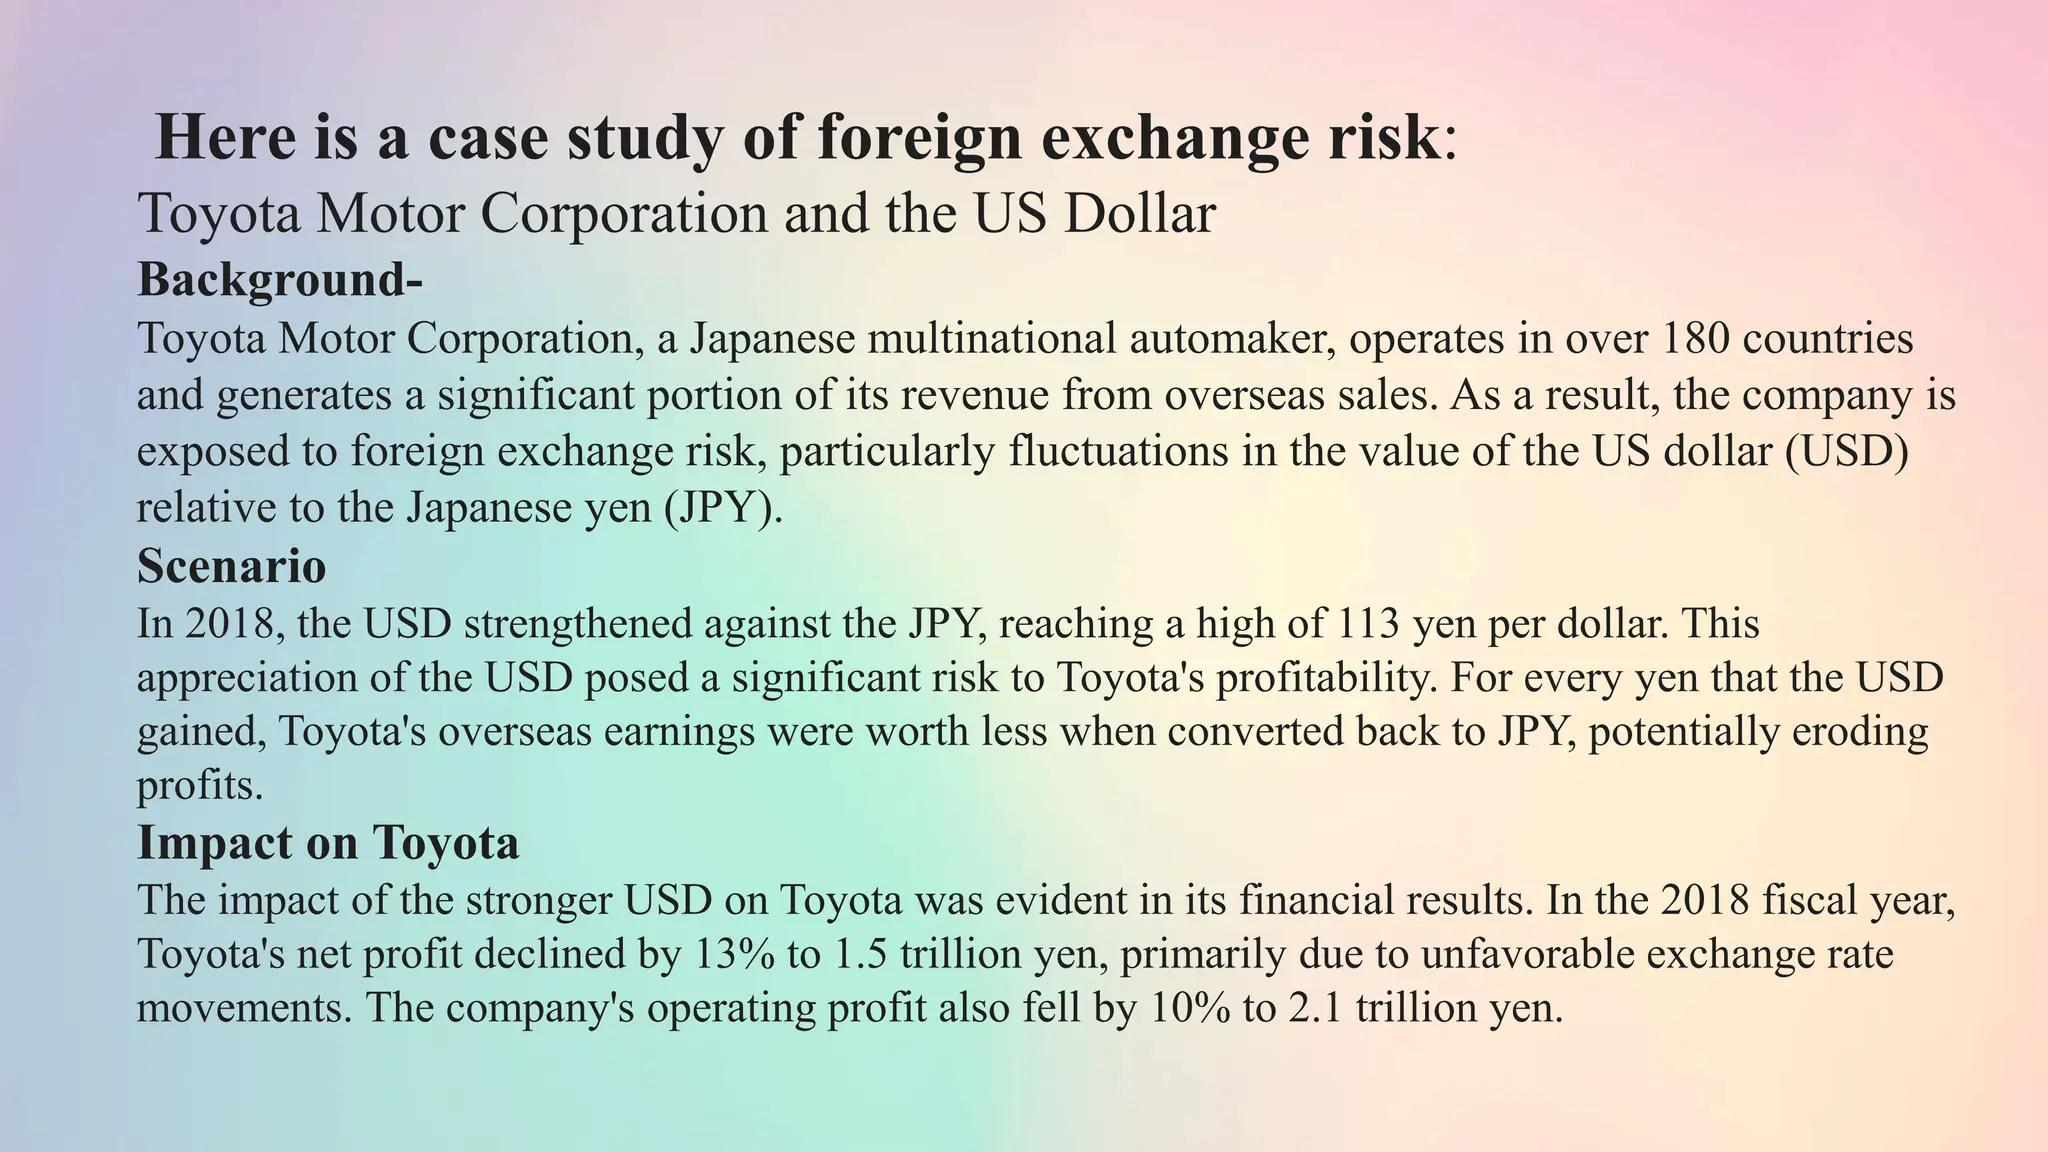
\includegraphics{figures/fig_0107.jpeg}
\textgreater{} OCR cue: Here is a case study of foreign exchange risk:
Toyota Motor Corporation and the US Dollar Background- Toyota Motor
Corporation, a Japanese multinational automaker, operates in over 180
countries and generates a significant portion of its revenue from
overseas sales. As a result, the company is exposed to foreign exchange
risk, particularly fluctuations in the value of the US dollar (USD)
relative

\hypertarget{figure-9-page-12}{%
\subsubsection{Figure 9 (Page 12)}\label{figure-9-page-12}}

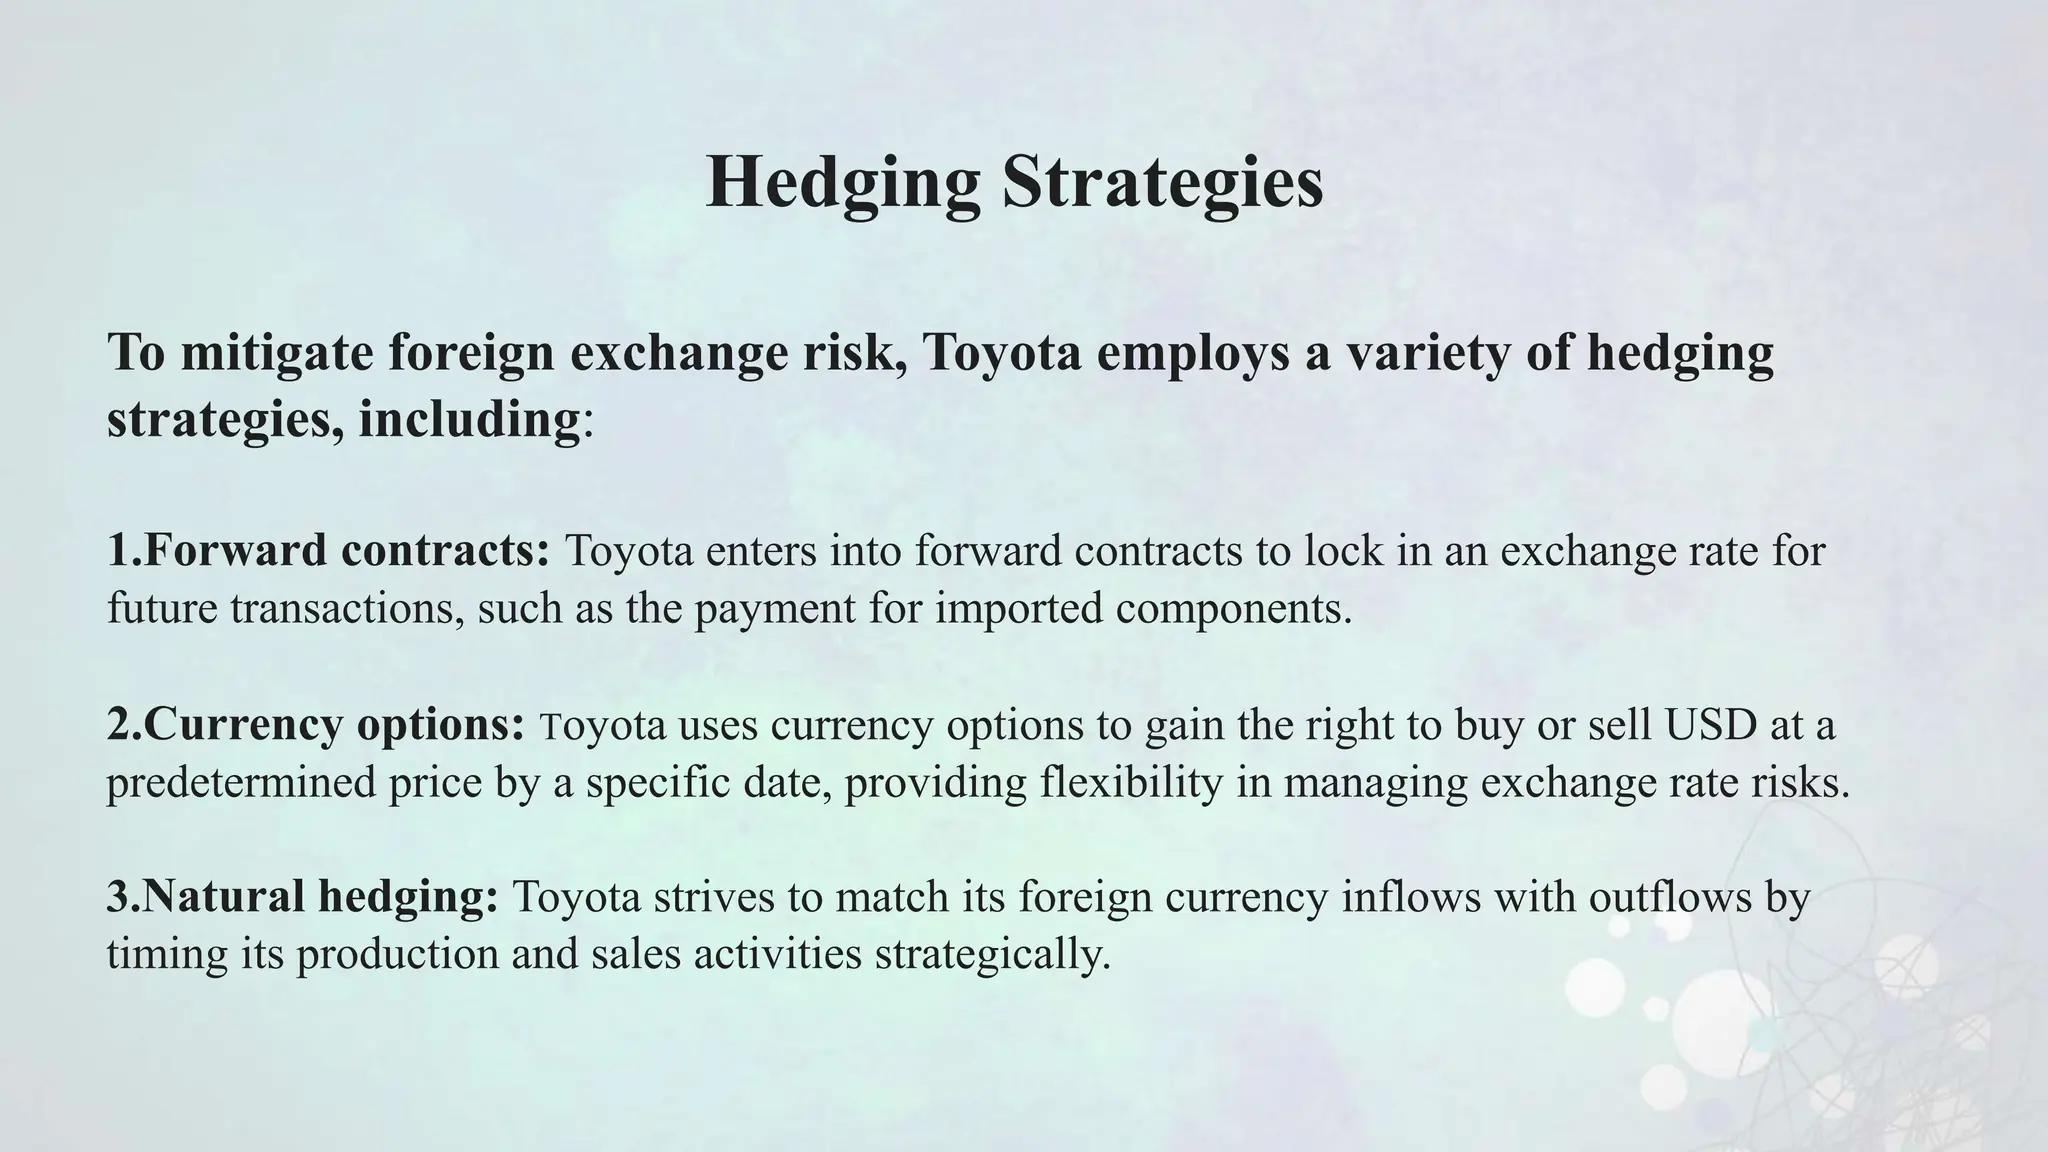
\includegraphics{figures/fig_0108.jpeg}
\textgreater{} OCR cue: Hedging Strategies To mitigate foreign exchange
risk, Toyota employs a variety of hedging strategies, including:
1.Forward contracts: Toyota enters into forward contracts to lock in an
exchange rate for future transactions, such as the payment for imported
components. 2.Currency options: Toyota uses currency options to gain the
right to buy or sell USD at a predetermined price by a specific date,

\hypertarget{figure-10-page-13}{%
\subsubsection{Figure 10 (Page 13)}\label{figure-10-page-13}}

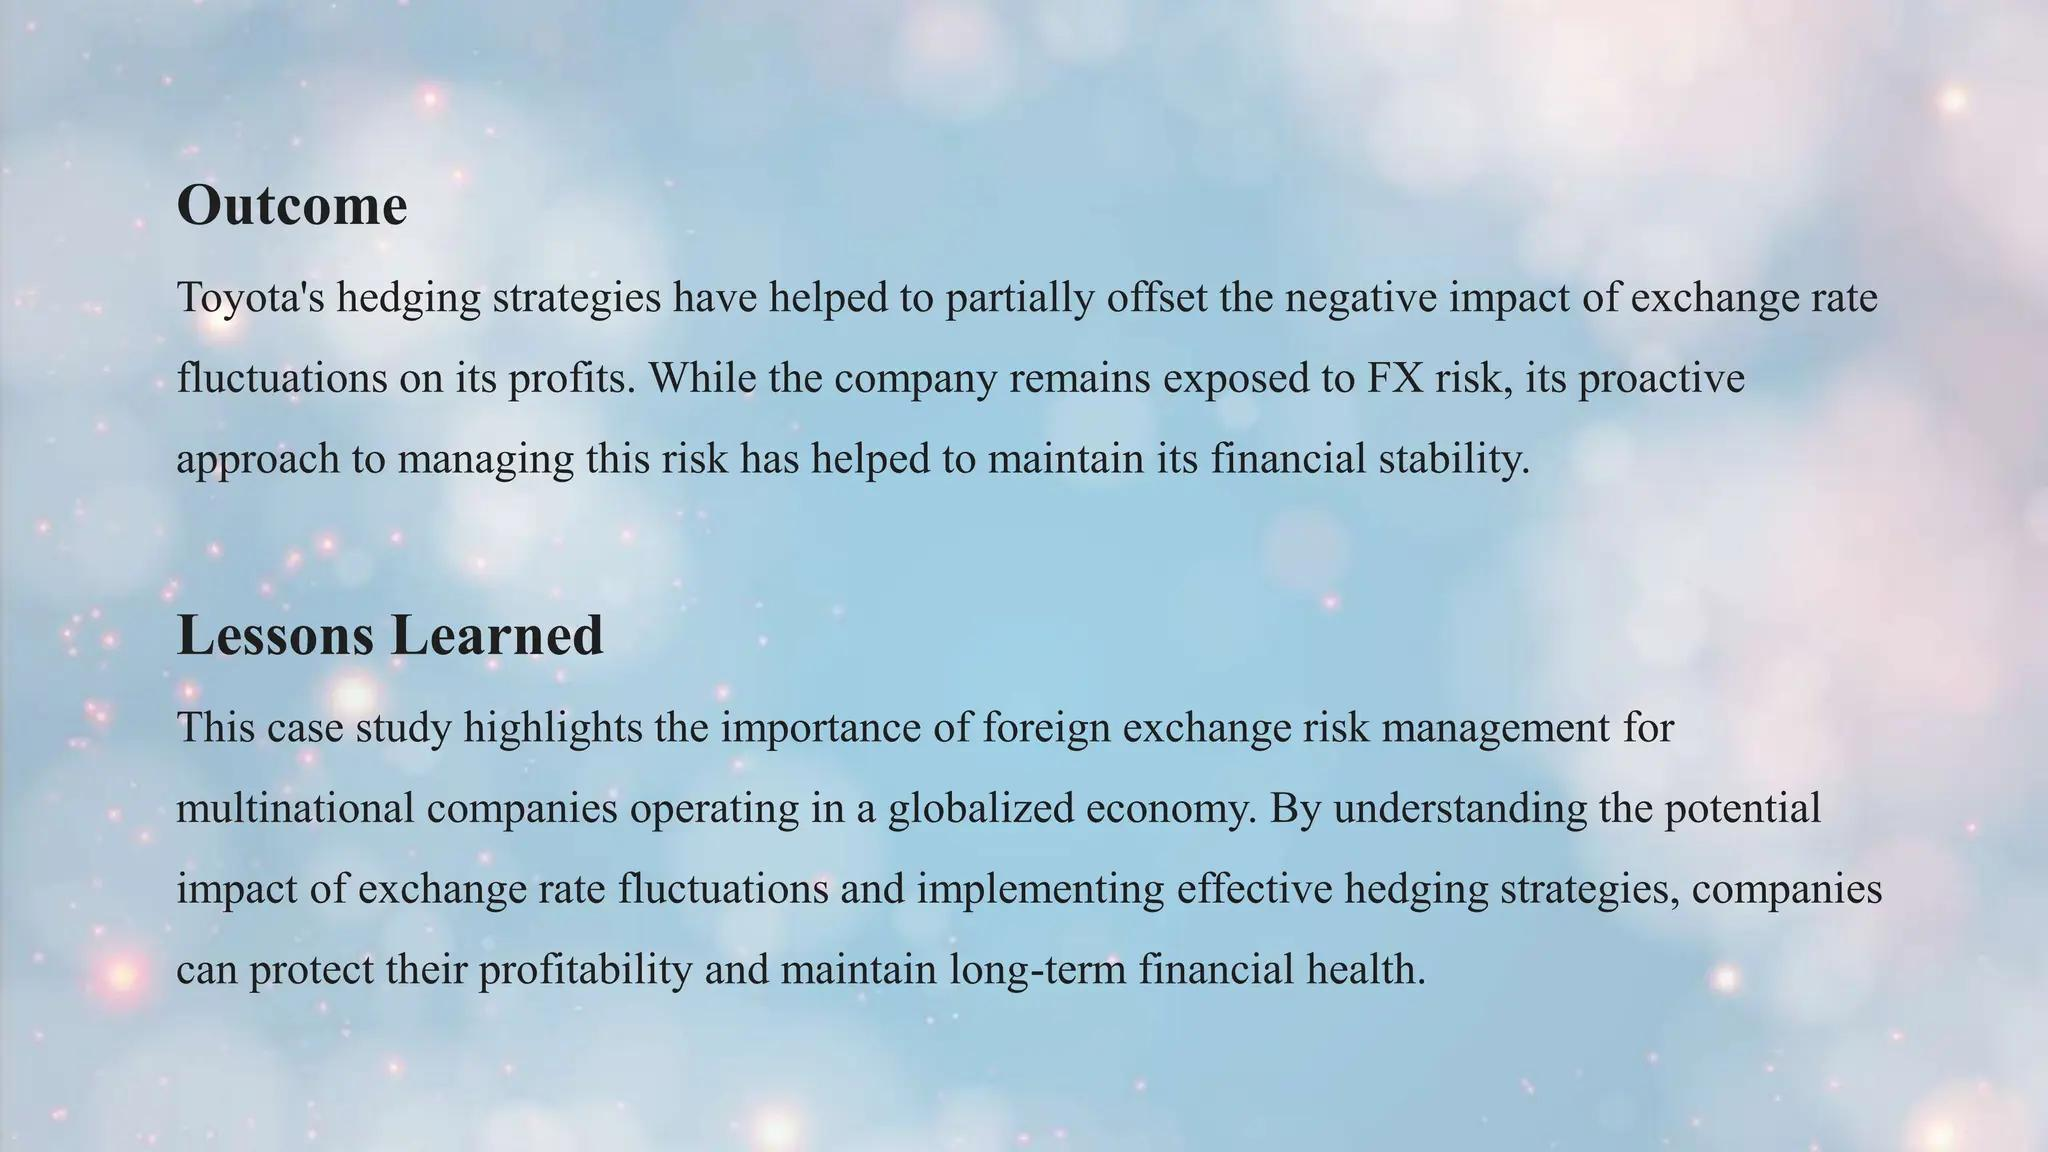
\includegraphics{figures/fig_0109.jpeg}
\textgreater{} OCR cue: Outcome Toyota's hedging strategies have helped
to partially offset the negative impact of exchange rate fluctuations on
its profits. While the company remains exposed to FX risk, its proactive
approach to managing this risk has helped to maintain its financial
stability. Lessons Learned This case study highlights the importance of
foreign exchange risk management for multinational companies opera

\hypertarget{figure-11-page-14}{%
\subsubsection{Figure 11 (Page 14)}\label{figure-11-page-14}}

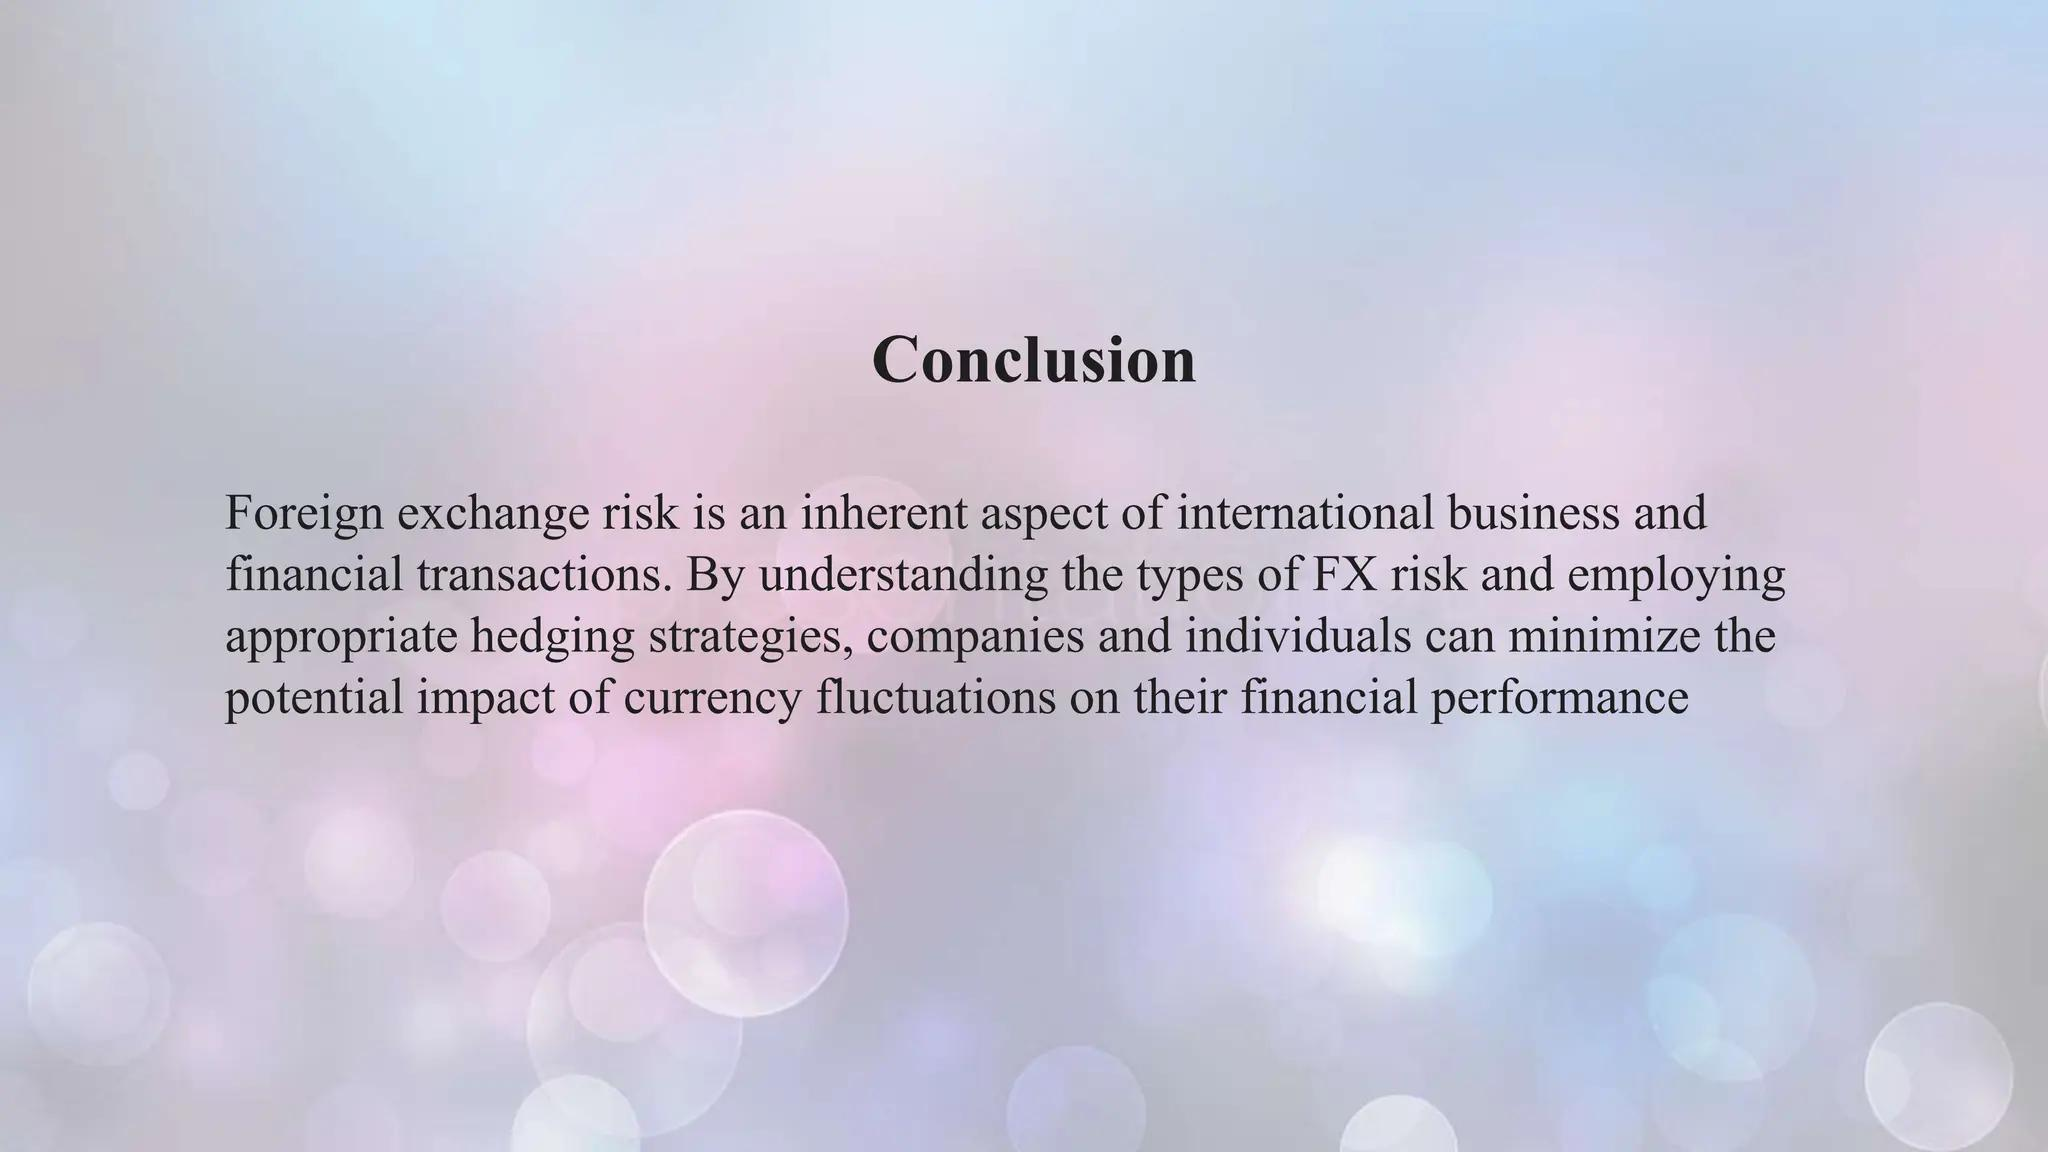
\includegraphics{figures/fig_0110.jpeg}
\textgreater{} OCR cue: Conclusion Foreign exchange risk is an inherent
aspect of international business and financial transactions. By
understanding the types of FX risk and employing appropriate hedging
strategies, companies and individuals can minimize the potential impact
of currency fluctuations on their financial performance

\hypertarget{unit-64-bond-strategy.pptx}{%
\subsection{UNIT 6/4 Bond
Strategy.pptx}\label{unit-64-bond-strategy.pptx}}

\hypertarget{figure-1-slide-1-2}{%
\subsubsection{Figure 1 (Slide 1)}\label{figure-1-slide-1-2}}

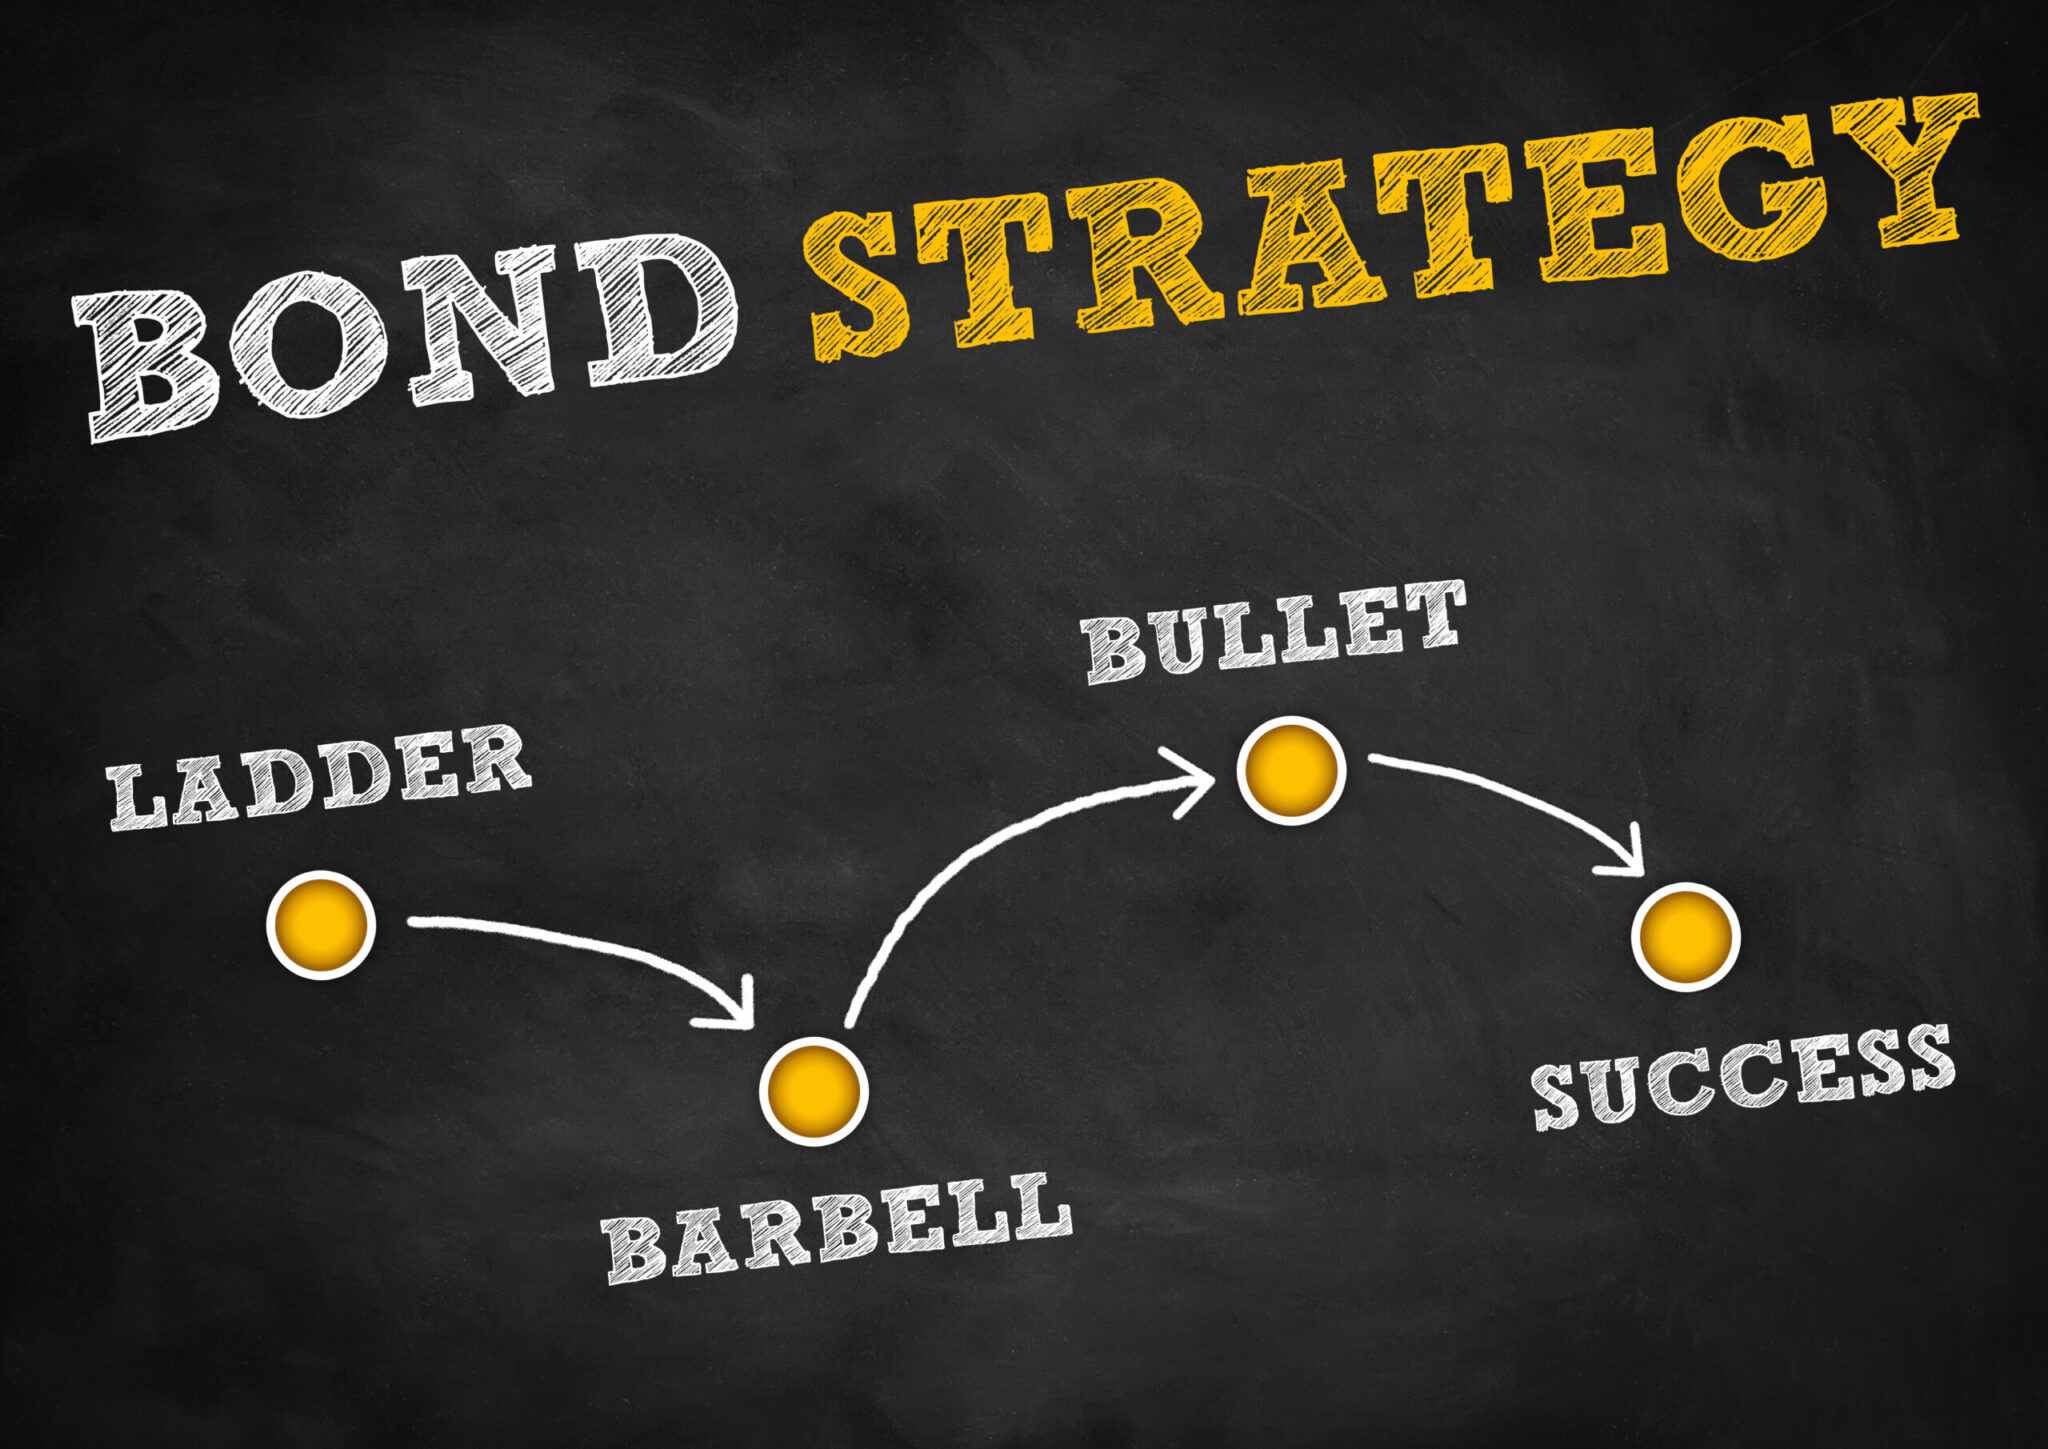
\includegraphics{figures/fig_0111.png}

\hypertarget{figure-2-slide-3-1}{%
\subsubsection{Figure 2 (Slide 3)}\label{figure-2-slide-3-1}}

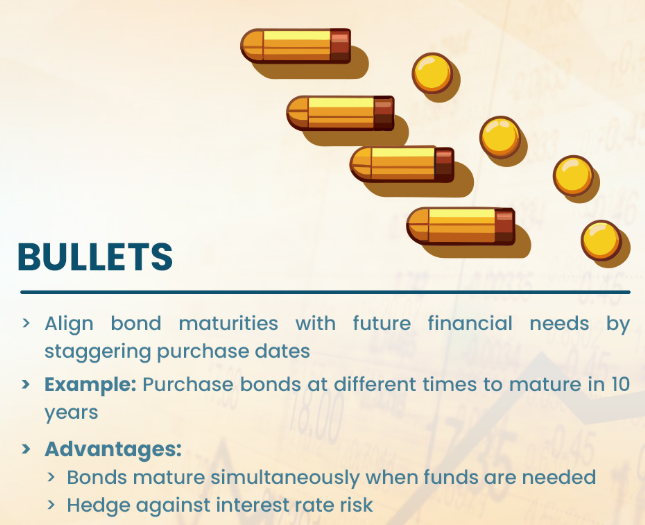
\includegraphics{figures/fig_0112.png}
\textgreater{} OCR cue: \textgreater{} Align bond maturities with future
financial needs by staggering purchase dates BULLETS \textgreater{}
Example: Purchase bonds at different times to mature in 10 years
\textgreater{} Advantages: \textgreater{} Bonds mature simultaneously
when funds are needed \textgreater{} Hedge against interest rate risk

\hypertarget{figure-3-slide-5}{%
\subsubsection{Figure 3 (Slide 5)}\label{figure-3-slide-5}}

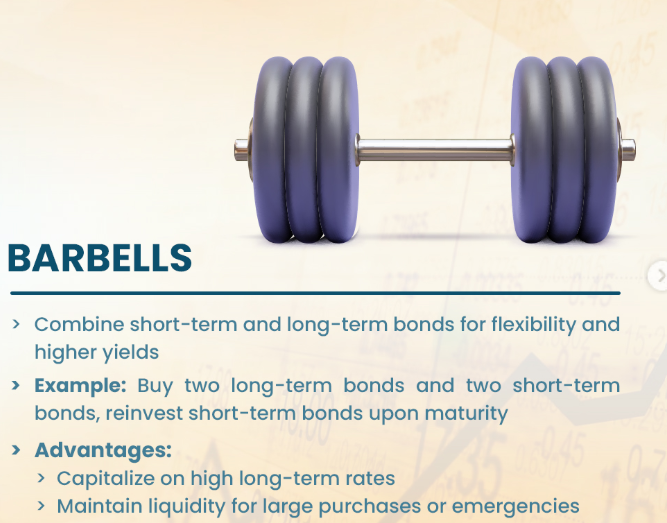
\includegraphics{figures/fig_0113.png}
\textgreater{} OCR cue: BARBELLS \textgreater{} Combine short-term and
long-term bonds for flexibility and higher yields \textgreater» Example:
Buy two long-term bonds and two short-term bonds, reinvest short-term
bonds upon maturity \textgreater{} Advantages: \textgreater{} Capitalize
on high long-term rates \textgreater{} Maintain liquidity for large
purchases or emergencies

\hypertarget{figure-4-slide-7-1}{%
\subsubsection{Figure 4 (Slide 7)}\label{figure-4-slide-7-1}}

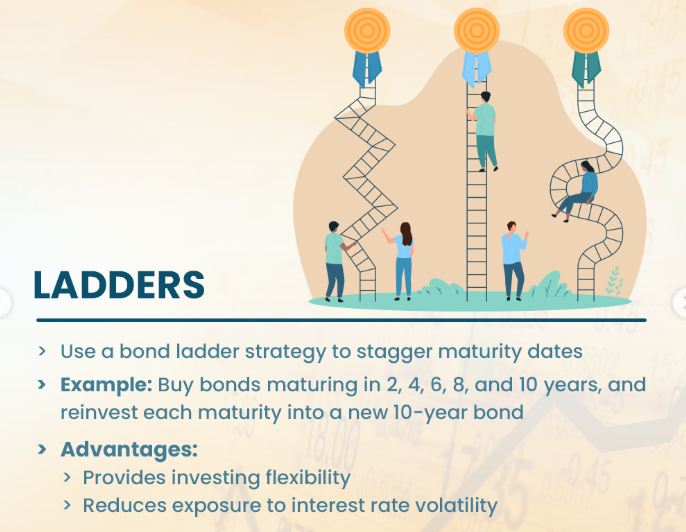
\includegraphics{figures/fig_0114.png}
\textgreater{} OCR cue: LADDERS \textgreater{} Use a bond ladder
strategy to stagger maturity dates \textgreater{} Example: Buy bonds
maturing in 2, 4, 6, 8, and 10 years, and reinvest each maturity into a
new 10-year bond \textgreater{} Advantages: \textgreater{} Provides
investing flexibility \textgreater{} Reduces exposure to interest rate
volatility

\hypertarget{figure-5-slide-9}{%
\subsubsection{Figure 5 (Slide 9)}\label{figure-5-slide-9}}

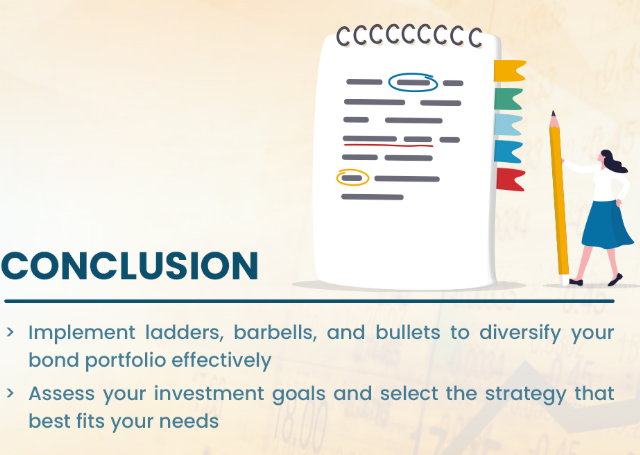
\includegraphics{figures/fig_0115.png}
\textgreater{} OCR cue: ccccccccc ee o---\_--- CONCLUSION \textgreater{}
Implement ladders, barbells, and bullets to diversify your bond
portfolio effectively \textgreater{} Assess your investment goals and
select the strategy that best fits your needs

\hypertarget{unit-64-hedging.pptx}{%
\subsection{UNIT 6/4 Hedging.pptx}\label{unit-64-hedging.pptx}}

\hypertarget{figure-1-slide-4}{%
\subsubsection{Figure 1 (Slide 4)}\label{figure-1-slide-4}}

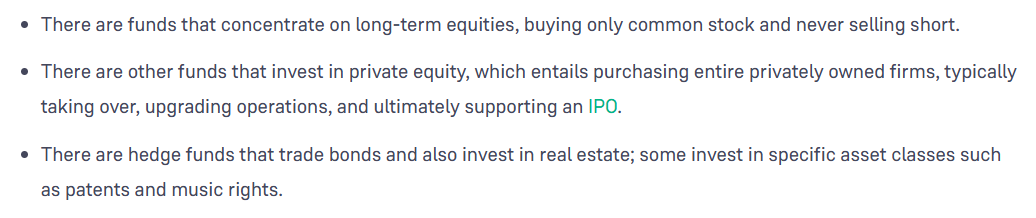
\includegraphics{figures/fig_0116.png} \textgreater{}
OCR cue: © There are funds that concentrate on long-term equities,
buying only common stock and never selling short. © There are other
funds that invest in private equity, which entails purchasing entire
privately owned firms, typically taking over, upgrading operations, and
ultimately supporting an IPO. © There are hedge funds that trade bonds
and also invest in real estate; some invest in specific asset

\hypertarget{figure-2-slide-5-1}{%
\subsubsection{Figure 2 (Slide 5)}\label{figure-2-slide-5-1}}

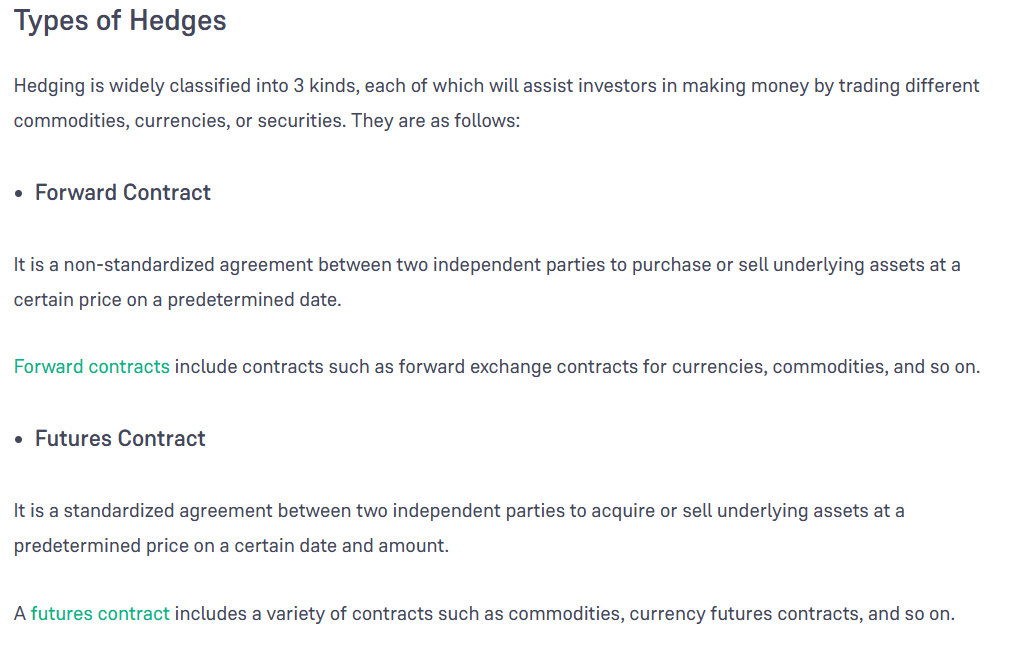
\includegraphics{figures/fig_0117.png} \textgreater{}
OCR cue: Types of Hedges Hedging is widely classified into 3 kinds, each
of which will assist investors in making money by trading different
commodities, currencies, or securities. They are as follows: ¢ Forward
Contract It is a non-standardized agreement between two independent
parties to purchase or sell underlying assets at a certain price on a
predetermined date. Forward contracts include contracts suc

\hypertarget{figure-3-slide-6-2}{%
\subsubsection{Figure 3 (Slide 6)}\label{figure-3-slide-6-2}}

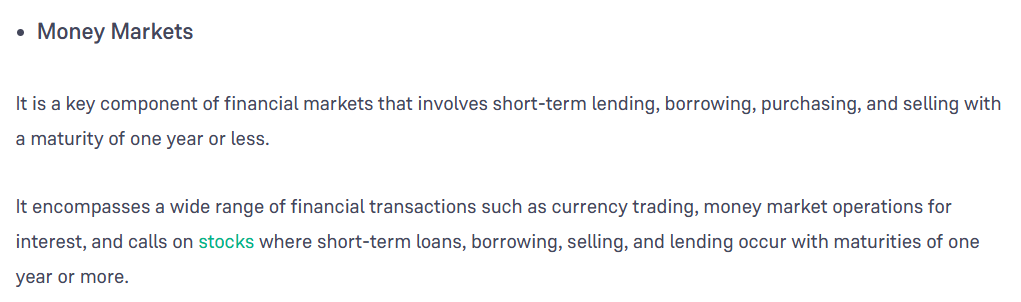
\includegraphics{figures/fig_0118.png} \textgreater{}
OCR cue: ¢ Money Markets It is a key component of financial markets that
involves short-term lending, borrowing, purchasing, and selling with a
maturity of one year or less. It encompasses a wide range of financial
transactions such as currency trading, money market operations for
interest, and calls on stocks where short-term loans, borrowing,
selling, and lending occur with maturities of one year or more

\hypertarget{figure-4-slide-7-2}{%
\subsubsection{Figure 4 (Slide 7)}\label{figure-4-slide-7-2}}

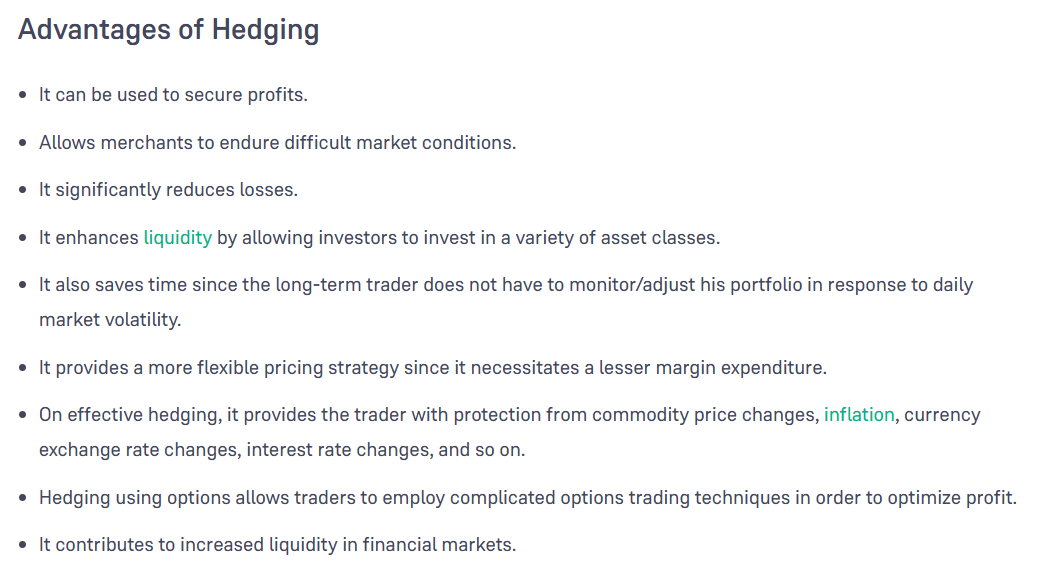
\includegraphics{figures/fig_0119.png} \textgreater{}
OCR cue: Advantages of Hedging It can be used to secure profits. Allows
merchants to endure difficult market conditions. It significantly
reduces losses. It enhances liquidity by allowing investors to invest in
a variety of asset classes. It also saves time since the long-term
trader does not have to monitor/adjust his portfolio in response to
daily market volatility. It provides a more flexible pricing st

\hypertarget{figure-5-slide-8}{%
\subsubsection{Figure 5 (Slide 8)}\label{figure-5-slide-8}}

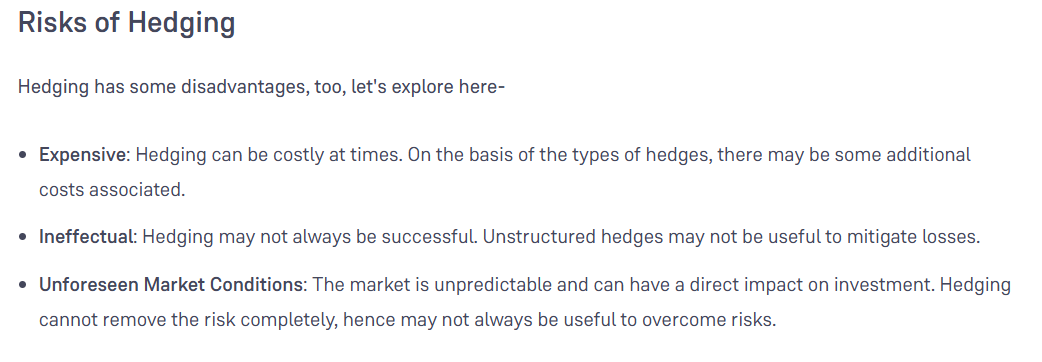
\includegraphics{figures/fig_0120.png} \textgreater{}
OCR cue: Risks of Hedging Hedging has some disadvantages, too, let's
explore here- e Expensive: Hedging can be costly at times. On the basis
of the types of hedges, there may be some additional costs associated. ¢
Ineffectual: Hedging may not always be successful. Unstructured hedges
may not be useful to mitigate losses. e Unforeseen Market Conditions:
The market is unpredictable and can have a direct impa

\hypertarget{figure-6-slide-9}{%
\subsubsection{Figure 6 (Slide 9)}\label{figure-6-slide-9}}

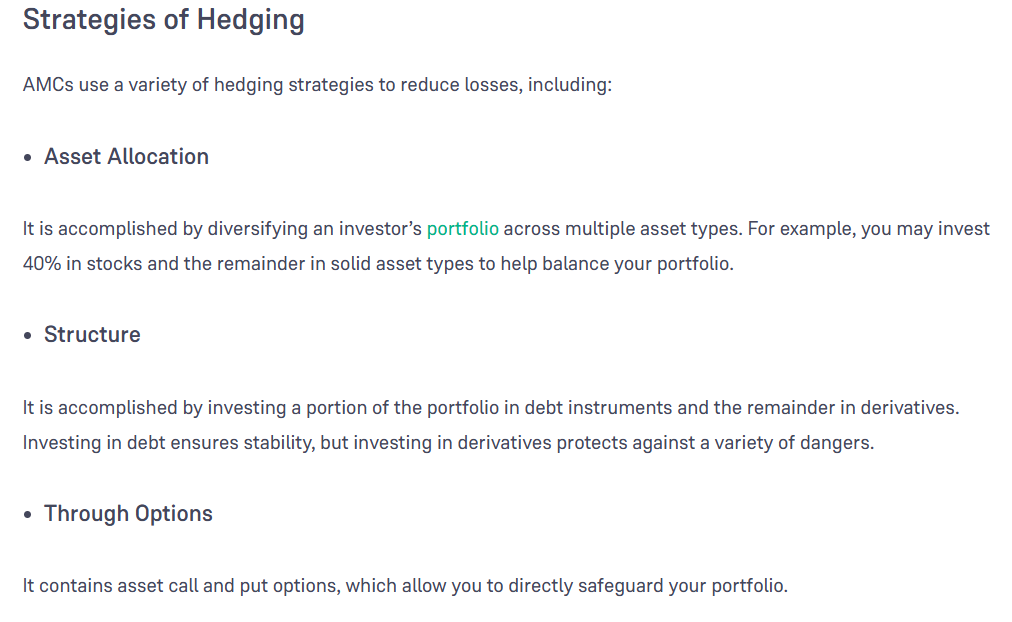
\includegraphics{figures/fig_0121.png} \textgreater{}
OCR cue: Strategies of Hedging AMCs use a variety of hedging strategies
to reduce losses, including: ¢ Asset Allocation It is accomplished by
diversifying an investor's portfolio across multiple asset types. For
example, you may invest 40\% in stocks and the remainder in solid asset
types to help balance your portfolio. ¢ Structure It is accomplished by
investing a portion of the portfolio in debt instrumen

\hypertarget{figure-7-slide-10}{%
\subsubsection{Figure 7 (Slide 10)}\label{figure-7-slide-10}}

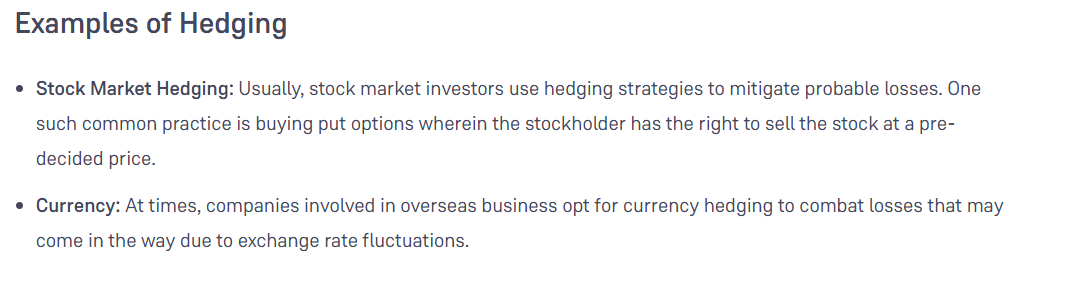
\includegraphics{figures/fig_0122.png} \textgreater{}
OCR cue: Examples of Hedging * Stock Market Hedging: Usually, stock
market investors use hedging strategies to mitigate probable losses. One
such common practice is buying put options wherein the stockholder has
the right to sell the stock at a pre- decided price. Currency: At times,
companies involved in overseas business opt for currency hedging to
combat losses that may come in the way due to exchange r

\end{document}
